\documentclass[10pt]{article}
\usepackage[polish]{babel}
\usepackage[utf8]{inputenc}
\usepackage[T1]{fontenc}
\usepackage{amsmath}
\usepackage{amsfonts}
\usepackage{amssymb}
\usepackage[version=4]{mhchem}
\usepackage{stmaryrd}
\usepackage{graphicx}
\usepackage[export]{adjustbox}
\graphicspath{ {./images/} }
\usepackage{bbold}
\usepackage{hyperref}
\hypersetup{colorlinks=true, linkcolor=blue, filecolor=magenta, urlcolor=cyan,}
\urlstyle{same}
\usepackage{multirow}

\title{MATEMATYKA }

\author{}
\date{}


\newcommand\Varangle{\mathop{{<\!\!\!\!\!\text{\small)}}\:}\nolimits}

\begin{document}
\maketitle
\section*{I KLASA GIMNAZJUM}
Bogdańska Beata\\
Maczan Aleksandra\\
Staniewska Iwona\\
Szuman Michał

\section*{Spis treści}
1 ZADANIA TEKSTOWE ..... 3\\
2 DZIAŁANIA NA LICZBACH ..... 17\\
2.1 Liczby naturalne ..... 17\\
2.2 Liczby całkowite ..... 24\\
2.3 Liczby wymierne ..... 30\\
2.4 Notacja wykładnicza zapisu liczb ..... 38\\
2.5 Dodatkowe tematy ..... 44\\
2.5.1 Wartość bezwzględna liczby ..... 44\\
2.5.2 Część całkowita liczby ..... 46\\
2.5.3 Część ułamkowa liczby ..... 47\\
2.5.4 Algorytm Euklidesa ..... 47\\
3 JEDNOSTKI W FIZYCE ..... 51\\
2.1 Czas ..... 51\\
2.2 Odległość, długość ..... 52\\
2.3 Prędkość ..... 53\\
2.4 Powierzchnia ..... 58\\
2.5 Objętość ..... 59\\
2.6 Masa ..... 59\\
3 UKŁAD WSPÓŁRZĘDNYCH ..... 62\\
4 POTĘGI I JEDNOMIANY ..... 77\\
4.1 Iloczyn potęg o równej podstawie ..... 78\\
4.2 Iloraz potęg o równej podstawie ..... 79\\
4.3 Potęga iloczynu i ilorazu ..... 80\\
4.4 Potęga potęgi ..... 81\\
4.5 Jednomiany ..... 83\\
4.6 Mnożenie jednomianów ..... 85\\
4.7 Dzielenie jednomianów ..... 86\\
5 WYRAŻENIA ALGEBRAICZNE ..... 88\\
5.1 Tworzenie wyrażeń algebraicznych ..... 88\\
5.2 Dodawanie (redukcja) jednomianów ..... 91\\
5.3 Dodawanie i odejmowanie sum alg. ..... 93\\
5.4 Iloczyn sumy alg. przez jednomian; wyłączanie jednomianu przed sumę ..... 95\\
5.5 Mnożenie sumy alg. przez sumę alg. ..... 99\\
5.6 Wzory skróconego mnożenia ..... 101\\
6 RÓWNANIA ..... 110\\
6.1 Rozwiązanie równania ..... 110\\
6.2 Rozwiązywanie równań ..... 111\\
6.3 Równania sprzeczne i tożsamościowe ..... 119\\
6.4 Wyznaczanie wskazanej wielkości z równania ..... 120\\
7 PROCENTY ..... 124\\
7.1 Wprowadzenie ..... 124\\
7.2 Wyznaczanie procentu liczby ..... 126\\
7.3 Wyznaczanie liczby z procentu ..... 127\\
7.4 Liczba jako procent drugiej liczby ..... 130\\
7.5 Zmiany/różnice procentowe ..... 134\\
7.6 Punkty procentowe ..... 141\\
8 ZADANIA TEKSTOWE ..... 145\\
9 NIERÓWNOŚCI ..... 160\\
10 UKEADY RÓWNAŃ ..... 168\\
11 GEOMETRIA ..... 183

\section*{Rozdział 1}
\section*{ZADANIA TEKSTOWE}
Ucząc sie matematyki realizujemy dwa podstawowe cele:

\begin{itemize}
  \item nabycie dobrej kontroli nad językiem polskim,
  \item wykształcenie umiejętności wnioskowania.
\end{itemize}

Obie te umiejętności są przydatne w życiu. Lepsza kontrola nad językiem oznacza poprawne rozumienie zdań języka polskiego oraz poprawne wyrażanie swoich myśli w języku polskim - to ostatnie jest trudną do opanowania umiejętnością.\\
Radzenie sobie z zadaniami w tym rozdziale sprowadza się do zrozumienia zdań języka polskiego i wywnioskowania co z nich wynika. Zadania są tak dobrane, że umiejętności arytmetyczne potrzebne do rozwiązywania tych zadań to poprawne wykonywanie działań na liczbach całkowitych.

\section*{PRZYKŁAD}
Adam ma 8 lat, a Bartek 12. Za ile lat będą oni mieli razem 44 lata?

\section*{Rozwiązanie}
Ile lat mają oni obecnie?

\[
8+12=20
\]

O ile zwiększy się suma ich lat w ciągu roku?

\[
\begin{aligned}
& (8+1)+(12+1)=22 \\
& 22-20=2
\end{aligned}
\]

Zatem suma ich lat zwiększy się w ciągu roku o 2 lata. Wobec tego mamy\\
\(44-20=24\)\\
\(24: 2=12\) bo co roku przybywają im łącznie 2 lata\\
Odpowiedź: oni będą mieli razem 44 lata za 12 lat.

\section*{PRZYKŁAD}
Adam i Bartek mają obecnie razem 18 lat. 3 lata temu Bartek był 5 razy starszy od Adama. Ile razy będzie Bartek starszy od Adama za 3 lata?

\section*{Rozwiązanie}
Jeżeli obecnie suma lat Adama i Bartka jest równa 18, to 3 lata temu, gdy każdy z nich był o 3 lata młodszy, suma ich lat była równa \(18-2 \cdot 3\) lat, czyli 12 lat. Bartek był wówczas 5 razy starszy, co oznacza, że Adam miał wówczas 2 lata, zaś Bartek 10 lat.\\
Wobec tego obecnie\\
Adam ma 5 lat, zaś Bartek 13 lat.\\
Zatem za 3 lata

\[
\begin{gathered}
\text { Adam będzie miał } 5+3=8 \text { lat, } \\
\text { a Bartek } 13+3=16 \text { lat }
\end{gathered}
\]

czyli za 3 lata Bartek będzie 2 razy starszy od Adama.

\begin{enumerate}
  \item 5 lat temu Ania i Kasia miały razem 15 lat, przy czym Kasia była wówczas 2 razy starsza od Ani. Ile lat ma Kasia obecnie?
  \item 8 lat temu syn miał 4 lata, a ojciec był 10 razy starszy od syna. Ile lat miał wtedy ojciec? Ile razy jest on obecnie starszy od syna?
  \item Jacek ma 11 lat, a Marek ma 1 rok. Ile lat będzie miał Jacek gdy będzie\\
a) 6 razy starszy od Marka?\\
b) 3 razy starszy od Marka?\\
c) 2 razy starszy od Marka?
  \item Jacek i Bartek mają razem 27 lat. Sześć lat temu Jacek był cztery razy starszy od Bartka. Ile lat ma teraz Bartek, a ile Jacek?
\end{enumerate}

W matematyce posługujemy się różnymi średnimi. W szkole poznaliśmy już średnią arytmetyczną. Przypomnijmy, że:\\
średniq arytmetyczna liczb nazywamy liczbę, która jest równa sumie tych liczb, podzielonej przez ich ilość. Na przykład średnia arytmetyczna następujących pięciu liczb: 10, 15, 18, 10, 22 jest równa 15 , bowiem

\[
\frac{10+15+18+10+22}{5}=\frac{75}{5}=15
\]

\section*{PRZYKŁAD}
Ania otrzymała z sześciu testów następujące wyniki: \(3,5,7,4,8,3\). Jaki wynik musi uzyskać z siódmego testu aby średni wynik z wszystkich siedmiu testów był równy 5?

\section*{Rozwiązanie}
Oznaczmy\\
\(x\) - poszukiwany wynik z siódmego testu.\\
Mamy wówczas

\[
\frac{3+5+7+4+8+3+x}{7}=5
\]

czyli

\[
\begin{aligned}
\frac{30+x}{7} & =5 \\
30+x & =35 \\
x & =5 .
\end{aligned}
\]

Odp: z siódmego testu Ania musi uzyskać dokładnie 5 punktów.\\
5. Bartek uzyskał z kolejnych testów następujące wyniki: 20, 16, 30, 24, 15, 27. Jaki był średni wynik Bartka z tych sześciu testów?\\
6. Ania otrzymała z pięciu testów wyniki \(4,5,4,6,2\). Jaki wynik musi otrzymać z szóstego testu, aby średnia wszystkich wyników była równa 5 ?\\
7. W klasie Ia jest 6 chłopców i 24 dziewczyny. Średnia waga jednego chłopaka wynosi 55 kg , a jednej dziewczyny 50 kg . Jaka jest średnia waga jednej osoby w tej klasie?\\
8. W klasie Ib jest 15 chłopców i 10 dziewcząt. Średnia waga jednego chłopaka wynosi 60 kg , a jednej dziewczyny 50 kg . Jaka jest średnia waga jednej osoby w tej klasie?\\
9. W klasie I a jest 29 uczniów. Średnia waga jednego ucznia wynosiła 45 kg . Gdyby liczyć średnią wagę wszystkich osób w klasie czyli wszystkich uczniów i nauczyciela, to średnia waga wynosiłaby 46 kg . Ile ważył nauczyciel?\\
10. Na statku było 31 marynarzy i kapitan. Średnia wieku marynarzy wynosiła 23 lata. Gdyby liczyć średnią wieku wszystkich marynarzy i kapitana, to wynosiłaby ona 24 lata. Ile lat ma kapitan?\\
11. Janek miał do przeczytania 600 stronicową książkę. Pierwszą połowę książki czytał on z prędkością 10 stron na dzień, a drugą połowę z prędkością 30 stron na dzień. Policz ile dni zajęło mu przeczytanie całej książki i ile wobec tego średnio stron dziennie czytał Janek.\\
12. Pies i gołąb mają razem 6 nóg, a głowy 2 . Ile nóg, a ile głów mają w sumie 4 gołębie i 3 psy?

\section*{PRZYKŁAD}
Na wybiegu w ZOO były strusie i antylopy. W sumie było 29 zwierząt. Gdy policzyliśmy ich nogi, to okazało się, że te zwierzęta mają w sumie 82 nogi. Ile antylop, a ile strusi było na wybiegu?

\section*{Rozwiązanie}
Gdyby każde zwierzę miało tylko 2 nogi, to wszystkich nóg byłoby \(29 \cdot 2=58\). W rzeczywistości nóg było 82 czyli o \(82-58=24\) więcej.\\
Te „dodatkowe" 24 nogi, są nogami antylop, które mają przecież po 4 nogi. Te „dodatkowe" 24 nogi należą zatem do \(24: 2=12\) antylop.

Odpowiedź: na wybiegu było 12 antylop i \(29-12=17\) strusi.\\
13. W ogrodzie były bażanty i króliki. Razem miały one 35 głów i 94 nogi. Ile królików, a ile bażantów było w ogrodzie? (bażanty są to ptaki; królik ma 4 nogi)\\
14. Na pastwisku pasą się krowy i gęsi. Zwierzęta te mają w sumie 18 głów i 50 nóg. Ile krów było na pastwisku?\\
15. Na parkingu stoją samochody i motocykle. Każdy samochód ma 5 kół (w tym jedno zapasowe) a każdy motocykl 2 koła. Wszystkich pojazdów było razem 19, a kół 59. Ile motocykli, a ile samochodów było na parkingu?

\section*{PRZYKŁAD}
Dwa zeszyty i trzy ołówki kosztują w sumie 4,20 zł.\\
Dwa zeszyty i cztery ołówki kosztują razem 4,60 zł.\\
Ile kosztuje jeden ołówek, a ile jeden zeszyt?

\section*{Rozwiązanie}
\section*{Oznaczmy}
\(z\) - cena 1 zeszytu\\
\(o\) - cena 1 ołówka.\\
Wówczas treść zadania można formalnie zapisać

\[
\begin{aligned}
& 2 \cdot z+3 \cdot o=4,20[\mathrm{zł}] \\
& 2 \cdot z+4 \cdot o=4,60[\mathrm{zł}]
\end{aligned}
\]

Z powyższych dwóch zdań wynika, że jeden ołówek kosztuje \(0,40 \mathrm{zł}\), zaś trzy\\
ołówki \(1,20 \mathrm{zł}\). Ponieważ dwa zeszyty i trzy ołówki kosztują razem \(4,20 \mathrm{zł}\), więc wobec tego dwa zeszyty kosztują \(3,00 \mathrm{zł}\), zaś jeden zeszyt kosztuje 1,50 zł.\\
Odpowiedź: 1 ołówek kosztuje 0,40 zł, zaś 1 zeszyt 1,50 zł.\\
Postępując podobnie rozwiąż poniższe zadania.\\
16. Trzy zeszyty i pięć ołówków kosztują razem 8,20 zł, natomiast trzy zeszyty i dziewięć ołówków 10,80 zł. Policz kolejno ile kosztują cztery ołówki, ile kosztuje jeden ołówek, ile kosztuje jeden zeszyt.\\
17. Jeden zeszyt i trzy ołówki kosztują razem 3,30 zł, zaś jeden zeszyt i pię́c ołówków kosztują razem 4,70zł. Ile kosztuje jeden zeszyt a ile jeden ołówek?

\section*{PRZYKŁAD}
2 bułki i chleb kosztują razem 4,70 zł. 7 bułek i 2 chleby kosztują razem 11,20 zł. Ile kosztuje bułka, a ile chleb?

\section*{Rozwiązanie}
Oznaczmy\\
\(b\) - cena bułki\\
\(c\) - cena chleba\\
Mamy wówczas

\[
\left\{\begin{array}{l}
2 b+c=4,70 \\
7 b+2 c=11,20
\end{array}\right.
\]

Z (1) wynika, że

\[
4 b+2 c=9,40
\]

Z (2) i (3) wynika, że

\[
3 b=1,80
\]

czyli

\[
b=0,60
\]

Wstawiajac to do (1) mamy

\[
2 \cdot 0,60+c=4,70
\]

czyli

\[
\begin{aligned}
& c=4,70-1,20 \\
& c=3,50
\end{aligned}
\]

Odpowiedź: chleb kosztuje 3,50,zł, a bułka 0,60 zł.\\
18. Ołówek i dwie gumki kosztują razem 1,90 zł, zaś dwa ołówki i pięć gumek kosztują 4,20 zł. Ile kosztuje gumka, a ile ołówek? Wsk. ile kosztują dwa ołówki i cztery gumki?\\
19. Trzy zeszyty i gumka kosztują razem 4 zł, zaś sześć zeszytów i trzy gumki kosztują razem \(8,40 \mathrm{zł}\). Ile kosztuje jedna gumka, a ile jeden zeszyt?\\
20. Dwa zeszyty i cztery ołówki kosztują razem 3,40 zł. Jeden zeszyt i jeden ołówek kosztują razem \(1,40 \mathrm{zł}\). Ile kosztuje jeden ołówek, a ile jeden zeszyt?\\
21. Trzy gumki i dwa zeszyty kosztują razem \(4,50 \mathrm{zl}\), zaś dziewięć gumek i siedem zeszytów kosztują razem 15 zł. Ile kosztuje gumka, a ile zeszyt?\\
22. Trzy gumki i pięć ołówków kosztują razem \(8,30 \mathrm{z}\), zaś dziewięć gumek i siedem ołówków - 14,50 zł. Ile kosztuje jedna gumka, a ile jeden ołówek?\\
23. Dwa zeszyty i piórnik kosztują razem 13,70 zł, natomiast cztery zeszyty i trzy piórniki kosztują razem \(38,90 \mathrm{zl}\). Ile kosztuje jeden piórnik, a ile jeden zeszyt?\\
24. Dwa zeszyty i trzy książki kosztują 13 złotych, a trzy zeszyty i dwie ksią̇̇iki 12 złotych. Z tego wynika, że\\
a) pięć zeszytów i pięć książek kosztuje razem ........... złotych\\
b) zeszyt i ksią̇̇ka kosztują razem ........... złotych\\
c) książka kosztuje ........... złotych\\
25. Zeszyt, gumka i ołówek kosztują razem 5 zł., zaś dwa zeszyty i dwie gumki kosztują razem 5,80 zł. Ile kosztuje ołówek?\\
26. Za zeszyt, długopis i książkę zapłacono razem 17 zł. Książka i długopis kosztują 15 zł. Zeszyt i ksią̇̇ka kosztują 14 zł. Policz kolejno ile kosztuje zeszyt, książka i długopis.

\section*{PRZYKŁAD}
Długopis i ołówek kosztują razem 4 zł.\\
Ołówek i pióro kosztują razem 13 zł.\\
Długopis i pióro kosztują razem 14 zł.\\
Ile kosztuje ołówek, ile długopis a ile pióro?

\section*{Rozwiązanie.}
Oznaczmy\\
\(d\) - cena długopisu\\
\(o\) - cena ołówka\\
\(p\) - cena pióra

Wobec tego mamy:

\[
\left\{\begin{aligned}
d+o & =4 \\
o+p & =13 \\
d+p & =14
\end{aligned}\right.
\]

Z (1), (2) i (3) wynika, że\\
2 długopisy, 2 ołówki i 2 pióra kosztują w sumie \(4+13+14=31\) zł czyli krótko

\[
2 d+2 o+2 p=31
\]

Wobec tego długopis, ołówek i pióro kosztują 15,50 zł.\\
Zatem\\
z (4) i (1) wynika, że \(p=15,50-4=11,50\)\\
z (4) i (2) wynika, że \(d=15,50-13=2,50\)\\
z (4) i (3) wynika, że \(o=15,50-14=1,50\)\\
27* Jacek kupił cztery książki. Druga, trzecia i czwarta książka kosztowały razem 42 złote, pierwsza, trzecia i czwarta kosztowały - 40 złotych, pierwsza druga i czwarta - 38 złotych, zaś pierwsza, druga i trzecia - 36 złotych. Ile kosztowała każda z tych czterech książek?\\
28. Koza, krowa, świnia i owca kosztują razem 1325 złotych. Koza, świnia i owca kosztują razem 425 złotych. Krowa, świnia i owca kosztują razem 1225 złotych. Koza i świnia kosztują razem 275 złotych. Ile kosztuje każde z tych zwierząt?

29* Obwód czworokąta ABCD jest równy 42 cm , obwód trójkąta BCD 32 cm , a trójkąta ABD - 24 cm . Jaka jest długość odcinka BD?\\
30* Prostokąt podzielono dwoma prostopadłymi odcinkami na cztery prostokąty, tak jak na rysunku obok. Obwód prostokąta \(A E G D\) jest równy 600 m , prostokąta EBCG 700 m , prostokata \(H F C D 800 \mathrm{~m}\), a prostokąta \(A B F H 900 \mathrm{~m}\). Wyznacz obwód prostokąta \(A B C D\). Wsk. w prostokącie równoległe boki są równej długości.\\
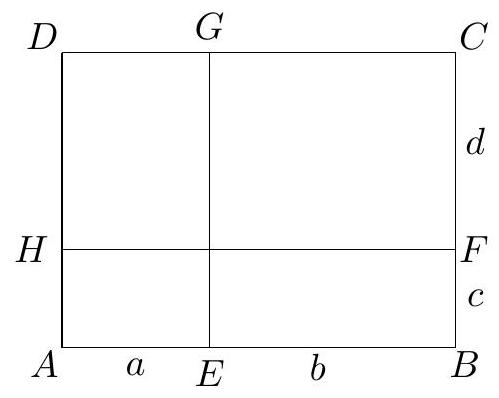
\includegraphics[max width=\textwidth, center]{2024_11_21_8f01584889ff06348ae7g-011}\\
31. Bartek i Wojtek mają razem 25 złotych, przy czym Bartek ma o 7 złotych więcej od Wojtka. Ile złotych ma Wojtek?\\
32. Adam i Bartek mają podzielić między siebie 140 złotych, przy czym Bartek ma otrzymać o 20 złotych więcej niż Adam. Ile złotych ma otrzymać Bartek?\\
33. Para butów i para skarpet kosztują razem 110 zł. Buty są o 100 zł droższe od skarpet. Ile kosztuje jedna para skarpet?\\
34. Dwie fontanny pobierają łącznie 72 litry wody na minutę, przy czym pierwsza z nich pobiera\\
a) 2 razy tyle wody co druga\\
b) 3 razy tyle wody co druga\\
c) 5 razy tyle wody co druga\\
d) 8 razy tyle wody co druga

Oblicz ile litrów wody pobiera na minutę pierwsza fontanna w każdym z powyższych czterech przypadków.

\section*{PRZYKŁAD}
Na obozie było 127 osób. Chłopców było o 33 więcej niż dziewcząt. Ile dziewcząt było na obozie?

\section*{Rozwiązanie}
Gdyby na obozie było o 33 chłopców mniej, to wówczas

\begin{itemize}
  \item chłopców i dziewczyn byłoby tyle samo,
  \item na obozie byłyby \(127-33=94\) osoby.
\end{itemize}

Z tego wynika, że na obozie było \(94: 2=47\) dziewcząt oraz \(47+33=80\) chłopców.\\
35. W szkole jest 429 uczniów. Chłopców jest o 27 więcej niż dziewcząt. Ile dziewcząt jest w szkole?\\
36. Mama i córka mają w sumie 71 lat. Mama jest o 25 lat starsza od córki. Ile lat ma córka, a ile matka?\\
37. Adam i Bartek mają w sumie 426 znaczków. Bartek ma o 44 znaczki mniej niż Adam. Ile znaczków ma Adam, a ile Bartek?\\
38. Na parkingu były 253 pojazdy: samochody i motocykle. Ile samochodów, a ile motocykli było na parkingu?\\
39. W klasie jest 28 uczniów. Część z nich dojeżdża do szkoły tramwajem a część chodzi do szkoły pieszo. Uczniów dojeżdżających tramwajem jest o 4 więcej niż uczniów chodzących do szkoły pieszo. Ilu uczniów chodzi do szkoły pieszo?\\
40. Podziel 90 znaczków pomiędzy Adama i Bartka, tak aby\\
a) Bartek miał 44 razy więcej znaczków niż Adam;\\
b) Bartek miał o 44 znaczki więcej niż Adam.\\
41. Podziel 100 złotych pomiędzy Adama i Marka, tak aby\\
a) Marek miał 49 razy więcej pieniędzy od Adama;\\
b) Marek miał o 49 złotych więcej od Adama.\\
42. Pojemnik zawierał 60 litrów płynu. Po pewnym czasie w pojemniku zostało 5 razy mniej płynu niż było na początku. Ile litrów płynu zużyto?\\
43. Duży zeszyt kosztuje o 15 gr więcej niż mały zeszyt. Ile kosztuje duży zeszyt, jeżeli 5 dużych zeszytów kosztuje tyle samo co 8 małych zeszytów?\\
44. Rozdziel 91 cukierków pomiędzy 10 dzieci tak, aby troje spośród nich otrzymało porcje dwa razy większe od każdego z pozostałych siedmiorga dzieci.\\
45. Paweł zamierzał kupić 4 porcje lodów, zabrakło mu jednak 80 groszy. Kupił więc 3 porcje, a wtedy pozostało mu 30 groszy. Jaka była cena jednej porcji lodów?\\
46. Jacek kupił 3 ciastka z kremem oraz 6 razy tyle ciastek z bitą śmietaną. Następnie wszystkie te ciastka rozdał (po jednym) swoim kolegom i koleżankom z klasy. Część osób odmówiła poczęstunku. Tych, którzy odmówili było 3 razy mniej od tych, którzy wzięli jakieś ciastko. Jacek dla siebie nie zachował żadnego ciastka. Ile osób liczy klasa Jacka?\\
47. Na talerzu leżały cukierki. Przyszedł Adam wziął połowę cukierków i wtedy okazało się, że na talerzu zostało 6 cukierków. Ile cukierków było początkowo na talerzu?\\
48. W koszyku były jabłka. Gdy przyszła Gosia i wzięła połowę wszystkich jabłek i jeszcze 2 jabłka, to w koszyku zostało 6 jabłek. Ile jabłek było początkowo w koszyku?\\
49. Na stole leżały cukierki. Przyszedł Jacek, wziął połowę wszystkich cukierków i jeszcze 4 cukierki. Następnie przyszedł Paweł i wziął pozostałych 7 cukierków. Ile cukierków było początkowo na stole?\\
50. Sprzedawczyni sprzedała pierwszej osobie połowę wszystkich jajek i jeszcze 2 jajka. Drugiej osobie sprzedała połowę reszty jajek i jeszcze jedno jajko. Po tej drugiej sprzedaży pozostało jej 8 jajek. Ile jajek miała ona początkowo? Ile jajek kupiła pierwsza, a ile druga osoba?\\
51. Na stole leżały cukierki. Przyszedł Adam i wziął połowę wszystkich cukierków. Następnie przyszedł Bartek i wziął połowę z pozostałych cukierków i jeszcze 2 cukierki. Pozostałe 4 cukierki wziął Czesiek. Ile cukierków było początkowo na stole?\\
52. Na talerzu leżały cukierki. Gosia wzięła dwie trzecie tych cukierków i jeszcze 2 cukierki. Pozostałe 4 cukierki wzięła Celina. Ile cukierków było początkowo na talerzu?\\
53. W koszyku były jabłka. Wpierw Gosia wzięła połowę tych jabłek. Potem Kasia wzięła jedną trzecią tego co zostało. Wtedy okazało się, że w koszyku zostało 6 jabłek. Ile jabłek było początkowo w koszyku?\\
54. W koszyku były jabłka. Wpierw Gosia wzięła połowę tych jabłek i jeszcze 2 jabłka. Następnie Krysia wzięła połowę z tego co pozostawiła Gosia i jeszcze 3 jabłka. W końcu Basia wzięła jedną trzecią z tego co pozostawiła Krysia. Wówczas okazało się, że w koszyku pozostały 2 jabłka. Ile jabłek było początkowo w koszyku?\\
55. Na stole leżały cukierki. Przyszedł Adam, wziął połowę wszystkich cukierków i jeszcze 1 cukierka. Następnie przyszedł Bartek i też wziął połowę leżących na stole cukierków i jeszcze 1 cukierka. W końcu przyszedł Czesiek i wziął ostatnich 9 cukierków. Ile cukierków leżało początkowo na stole?\\
56. Na stole leżały cukierki. Przyszedł Adam, wziął połowę wszystkich cukierków i jeszcze 2 cukierki. Następnie przyszedł Bartek, wziął połowę z tych, które były na stole, cukierków i jeszcze 2 cukierki. Na końcu przyszedł Marek, wziął połowę z tych cukierków, które były na stole i jeszcze ostatnie 3 cukierki. Ile cukierków było początkowo na stole?\\
57. W koszyku były jabłka. Pierwsza osoba wzięła z koszyka połowę wszystkich jabłek i jeszcze jedno jabłko. Druga osoba wzięła połowę pozostałych jabłek i jeszcze jedno jabłko. Trzecia osoba wzięła połowę pozostałych jabłek i pozostałe trzy jabłka. Wtedy koszyk był pusty. Ile jabłek było na początku w tym koszyku?\\
58. W szufladzie jest 20 białych i 16 czarnych skarpet. Wyciągamy po ciemku skarpety z szuflady.\\
a) Ile skarpet wystarczy wyciągnąć, aby mieć pewność, że wśród nich jest jedna para tego samego koloru?\\
b) Ile skarpet wystarczy wyciągnąć, aby mieć pewność, że wśród wyciągniętych skarpet jest para białych skarpet?\\
c) Ile skarpet wystarczy wyciągnąć para skarpet każdego koloru?\\
59. W trzech torebkach są trzy gatunki cukierków. Z każdego gatunku jest 20 cukierków. Wsypaliśmy te cukierki do jednego pojemnika. Wyciągamy następnie z niego po ciemku cukierki. Ile cukierków wystarczy wyciągnąć, aby mieć pewność, że wśród nich są trzy cukierki jednego gatunku?\\
60. Do szuflady wrzuciliśmy 16 skarpet tego samego rozmiaru - 4 pary czarnych i 4 pary brazzowych. Wyciągamy po ciemku po jednej skarpecie z szuflady. Ile skarpet wystarczy wyciągnąć aby mieć pewność, że wśród nich jest:\\
a) jedna para skarpet tego samego koloru;\\
b) jedna para czarnych skarpet?\\
61. W szufladzie jest 29 jednakowego rozmiaru skarpet: 9 niebieskich, 8 zielonych i 12 czarnych. Wyciągamy po ciemku skarpety z szuflady. Ile skarpet wystarczy wyciągnąć, aby mieć pewność, że wśród nich jest\\
a) jedna para jednokolorowych skarpetek;\\
b) po jednej parze każdego koloru skarpetek;\\
c) jedna para niebieskich skarpetek?\\
d) skarpeta niebieska?\\
62. W pudełku znajdują się kule: 5 białych, 10 czerwonych i 15 niebieskich. Wyciągamy po ciemku kule. Jaką najmniejszą liczbę kul trzeba wyjąć, aby mieć pewność, że wśród wyciągniętych kul będzie\\
a) 5 kul jednego koloru?\\
b) 7 kul jednego koloru\\
c) 11 kul jednego koloru?\\
d) co najmniej po jednej kuli każdego koloru?\\
e) co najmniej po trzy kule każdego koloru?\\
63. W pudełku leżą kredki: 10 czerwonych, 8 niebieskich, 8 zielonych i 4 żółte. Wyciagamy po ciemku kredki z pudełka. Ile co najmniej kredek trzeba wyciągnąć, aby mieć pewność, że wśród wyciągniętych kredek\\
a) są 4 jednego koloru,\\
b) są kredki wszystkich kolorów,\\
c) jest co najmniej 6 kredek jednego koloru?\\
64. Adam jest w stanie przekopać działkę w ciągu 2 godzin, Bartek w ciągu 3 godzin, a Czesiek w ciągu 6 godzin. W jakim czasie przekopią oni wspólnie całą działkę?

65* Adam jest w stanie skopać działkę w ciągu 2 godzin, a Bartek w ciągu 3 godzin. W jakim czasie skopią oni działkę, jeżeli będą pracowali równocześnie?\\
Wsk. Jaką część działki skopie Adam w ciągu 1 godziny? Jaką część działki skopie Bartek w ciągu 1 godziny? Jaką część działki skopią Adam i Bartek razem w ciągu 1 godziny?

66* Pewną działkę Piotrek może przekopać w ciągu 15 godzin, Zbyszek w ciągu 12 godzin, a Michał w ciągu 10 godzin. Ile czasu zajmie im wspólnie przekopanie całej działki?

67* Mąż wypije przygotowany napój w ciągu 14 dni, a wspólnie z żoną wypiją ten napój w ciągu 10 dni. W ciągu ilu dni wypije ten napój żona?

68* Koza i krowa zjadają razem wóz siana w ciągu 45 dni. Krowa i owca w ciągu 60 dni, zaś owca i koza - w ciągu 90 dni. W ciągu ilu dni zjedzą wóz siana koza, owca i krowa razem?

69* Wiemy, że 12 robotników może wykonać pewną pracę w ciągu 25 dni. Po 5 dniach liczbę robotników zwiększono i pracę wykonano w 4 dni przed terminem. Ilu robotników przystąpiło dodatkowo do pracy?\\
70. W klasie jest 20 uczniów. Połowa z nich gra w koszykówkę. Dwie piąte gra w siatkówkę, przy czym jedna dziesiąta gra zarówno w koszykówkę jak i w siatkówkę. Ilu uczniów w tej klasie nie gra w żadną z tych gier?\\
71. W 25 osobowej klasie 14 uczniów potrafi pływać, 9 potrafi grać w szachy, przy czym 2 potrafi zarówno pływać jak i grać w szachy. Ilu uczniów z tej klasy potrafi tylko pływać, a ilu nie potrafi ani pływać ani grać w szachy?

\section*{PRZYKŁAD}
10 kur w 10 dni znosi 60 jajek. Ile jajek zniesie 25 kur w 25 dni?

\section*{Rozwiązanie}
Z tego, że 10 kur w 10 dni znosi 60 jajek, wynika, że\\
1 kura w 10 dni znosi 6 jajek,\\
zaś\\
1 kura w 5 dni znosi 3 jajka.\\
Z tego wynika, że\\
1 kura w 25 dni znosi 15 jajek.\\
Z tego wynika, że\\
25 kur w 25 dni znosi 375 jajek.

Postępując w taki sam sposób i pisząc podobne komentarze, rozwiąż następnych pięć zadań.\\
72. 5 pająków łapie 5 much w ciągu 5 godzin. Ile much złapie 100 pająków w ciągu 100 godzin?\\
73. 10 kur w ciągu 10 dni znosi 50 jajek. Ile jajek znosi 20 kur w 20 dni?\\
74. 10 owiec w ciągu 10 dni zjada 360 kg siana. Ile siana zje 15 owiec w ciągu 20 dni?\\
75. 15 kur w 15 dni znosi 90 jajek. Ile jajek zniesie 25 kur w 25 dni?\\
76. 6 pająków w ciągu 4 godzin łapie 6 much. Ile much złapie 40 pająków w ciągu 40 godzin?

\section*{Odpowiedzi}
\begin{enumerate}
  \item 15 lat
  \item 75 kg
  \item ojciec miał 40 lat, obecnie jest 4
  \item 55 lat razy starszy,
  \item 40 dni, 15 stron na dzień
  \item a) 12 lat, b) 15 lat, c) 20 lat\\
12.7 głów, a 20 nóg
  \item Bartek 9 lat, Jacek 18 lat.
  \item 12 królików, 23 bażanty
  \item 22\\
14.7 krów\\
6.9
  \item 12 motocykli, 7 samochodów\\
7.51 kg
  \item zeszyt 1,65 zł, ołówek 0,65 zł\\
8.56 kg
  \item zeszyt \(1,20 \mathrm{zł}\), ołówek \(0,70 \mathrm{zł}\)
  \item gumka \(0,40 \mathrm{zł}\), ołówek \(1,10 \mathrm{zł}\)
  \item gumka \(0,40 \mathrm{zł}\), zeszyt \(1,20 \mathrm{zł}\)
  \item ołówek \(0,30 \mathrm{zł}\), zeszyt \(1,10 \mathrm{zł}\)
  \item gumka \(0,50 \mathrm{zl}\), zeszyt \(1,50 \mathrm{zł}\)
  \item gumka \(0,60 \mathrm{zł}\), ołówek \(1,30 \mathrm{zł}\)
  \item zeszyt \(1,10 \mathrm{zł}\), piórnik \(11,50 \mathrm{zł}\)
  \item a) 25 zl , b) \(5 \mathrm{zł}\), c) \(3 \mathrm{zł}\)
  \item 2,10 zł\\
26.z - \(2 \mathrm{zł}\) k - 12zł, d - 3zł, 27. pierwsza \(10 \mathrm{zł}\), druga 12 zl , trzecia 14 zl , czwarta \(16 \mathrm{zł}\)
  \item krowa 900 zl , świnia 175 zł, owca 150 zł, koza 100 zł\\
29.7 cm\\
30.1000 m
  \item Bartek 16 zł, Wojtek 9 zł
  \item Adam 60 zł, Bartek \(80 \mathrm{zł}\)
  \item skarpety \(5 \mathrm{zł}\), buty 105 zl
  \item a) 48 l , b) 54 l , c) 60 l d) 64 l
  \item dziewcząt - 201, chłopców -228
  \item pieszo - 12, tramwajem - 16
  \item Adam - 235, Bartek - 191
  \item 87 motocykli, 166 samochodów
  \item pieszo - 12, tramwajem - 16
  \item a) Bartek 88, a Adam 2, b) Bartek 67, a Adam 23
  \item a) Marek 98 zl , Adam \(2 \mathrm{zł}\), b) Adam 25,50 zł, Marek - 74,50 zł 42.48 litrów
  \item mały 25 gr, duży 40 gr
  \item troje dzieci po 14 cukierków, a siedmioro dzieci po 7 cukierków
  \item 1,10 zł
  \item 29 osób\\
47.12 cukierków\\
48.16 jabłek\\
49.22 cukierki\\
50.40 jajek\\
51.24 cukierki\\
\(\mathbf{5 2 . 1 8}\) cukierków\\
53.18 jabłek\\
\(\mathbf{5 4 . 2 8}\) jabłek\\
55.42 cukierki
  \item 36 cukierków
  \item 30 jabłek
  \item a) 3 , b) 18, c) 22\\
59.7 cukierków
  \item a) 3 skarpety, b) 10 skarpet
  \item a) 7 , b) 23 , c) 22 d) 21
  \item a) 13 , b) 18 , c) 26 , d) 26 , e) 28
  \item a) 13, b) 27 , c) 20
  \item w ciągu 1 godziny
  \item \(1 \frac{1}{5}\) godziny
  \item 4 godziny\\
67.35 dni
  \item 40 dni
\end{enumerate}

69 . 3 robotników\\
70.4 uczniów\\
71.12 tylko potrafi pływać, 4 nie potrafi ani pływać, ani grać w szachy 72. 2000 much, wsk. Ile much łapie 1 pająk w ciągu 5 godzin?\\
73. 200 jajek, wsk. Ile jajek zniesie 1 kura w ciągu 10 dni, a ile w ciągu 20 dni?\\
74.1080 kg\\
75.250 jajek\\
76. 400 much

\section*{Rozdział 2}
\section*{DZIAEANIA NA LICZBACH}
W tym rozdziale powtórzymy znane nam już wcześniej różne fakty o liczbach i o działaniach na nich. Wprowadzimy różne nowe pojęcia oraz pewne formalne symbole ułatwiajace matematykom porozumiewanie się.

\subsection*{2.1 Liczby naturalne}
Za najmniejszą liczbę naturalną będziemy przyjmować liczbę 1. Jest to tylko sprawa umowy. Część matematyków za najmniejszą liczbę naturalną przyjmuje 0, bo tak jest im wygodniej. Kolejnymi liczbami naturalnymi według naszej są zatem \(1,2,3, \ldots\) Te trzy kropki, które nie raz będziemy używać, oznaczają: i tak dalej. Zbiór liczb naturalnych będziemy oznaczać literą \(\mathbb{N}\). Wobec tego, krótko mówiąc

\[
\mathbb{N}=\{1,2,3, \ldots\}
\]

co na osi liczbowej możemy zilustrować następująco:\\
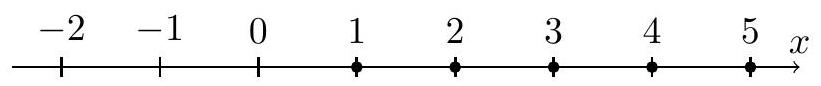
\includegraphics[max width=\textwidth, center]{2024_11_21_8f01584889ff06348ae7g-019}

\section*{UWAGA}
Zdanie „1 jest liczbą naturalną" zapisujemy w symbolice matematycznej następująco \(1 \in \mathbb{N}\). Symbol \(\in\) odczytujemy „należy do" czy też „jest elementem", zaś symbol \(\notin\) oznacza „nie nalė̇y". Na przykład \(-2 \notin \mathbb{N}\), co\\
odczytujemy: -2 nie nalė̇y do zbioru liczb naturalnych, lub też krócej -2 nie jest liczba naturalna.\\
Suma dwóch liczb naturalnych jest liczbą naturalną. Dodawanie liczb jest przemienne, co oznacza, że dla dowolnych liczb naturalnych \(a, b\)

\[
a+b=b+a
\]

Dodawanie liczb naturalnych jest łączne, co oznacza, że dla dowolnych liczb naturalnych \(a, b, c\)

\[
(a+b)+c=a+(b+c)
\]

Dlatego zamiast pisać \((a+b)+c\) lub też \(a+(b+c)\), piszemy krócej \(a+b+c\).

\section*{PRZYKŁAD}
\[
(37+49)+63=(37+63)+49=100+49=149
\]

\begin{enumerate}
  \item Korzystając z łączności i przemienności dodawania oblicz w pamięci\\
a) \((17+49)+13=\)\\
b) \((111+184)+189=\)\\
c) \((44+89)+36=\)\\
d) \((17+25)+(83+75)=\)\\
e) \((48+75)+252=\)\\
f) \((244+478)+156=\)\\
g) \(23+(49+77)=\)\\
h) \((34+108)+66=\)\\
i) \((325+49)+475=\)\\
j) \((211+46)+89=\)\\
k) \((405+38)+95=\)\\
l) \((133+98)+167=\)
\end{enumerate}

Podobnie rzecz się ma z działaniem mnożenia liczb naturalnych. Iloczyn dwóch dowolnych liczb naturalnych jest liczbą naturalną, a przy tym mnożenie, tak jak i dodawanie, jest przemienne i łączne, czyli dla dowolnych liczb naturalnych \(a, b, c\)

\[
\begin{aligned}
a \cdot b & =b \cdot a \\
(a \cdot b) \cdot c & =a \cdot(b \cdot c) .
\end{aligned}
\]

\section*{PRZYKŁAD}
\[
(2 \cdot 17) \cdot 5=(17 \cdot 2) \cdot 5=17 \cdot(2 \cdot 5)=17 \cdot 10=170
\]

\begin{enumerate}
  \setcounter{enumi}{1}
  \item Korzystając z łączności i przemienności mnożenia oblicz w pamięci\\
а) \((23 \cdot 2) \cdot 5=\)\\
b) \((3 \cdot 5) \cdot 2=\)\\
c) \((2 \cdot 13) \cdot 5=\)\\
d) \((7 \cdot 8) \cdot 5=\)\\
e) \((6 \cdot 9) \cdot 5=\)\\
f) \((17 \cdot 5) \cdot 2=\)\\
g) \((4 \cdot 17) \cdot 5=\)\\
h) \((13 \cdot 5) \cdot 4=\)\\
i) \((15 \cdot 3) \cdot 4=\)
\end{enumerate}

\section*{OKREŚLENIE}
Wielokrotnością liczby naturalnej \(a\) nazywamy każdą liczbę naturalną \(k \cdot a\), gdzie \(k\) oznacza liczbę naturalną.

\section*{PRZYKŁAD}
Wielokrotnościami liczby 3 większymi od 1 , ale mniejszymi od 17 są liczby \(3,6,9,12,15\).\\
3. Wypisz wielokrotności\\
a) liczby 2 większe od 5 a mniejsze od 18\\
b) liczby 5 większe od 11 a mniejsze od 36\\
c) liczby 7 większe od 14 a mniejsze od 54

W zbiorze liczb naturalnych wprowadzamy pojęcie: podzielność liczby przez liczbę. Przypomnijmy znaczenie tego pojęcia na przykładach.

\section*{PRZYKŁAD}
Liczba 6 jest podzielna przez 2 (lub też inaczej mówiąc 2 dzieli liczbę 6), co zapisujemy \(2 \mid 6\), bo 6 dzieli się bez reszty przez 2 , czyli \(6: 2=3\). Jednak dzielenie \(6: 2=3\) zachodzi tylko wtedy, gdy zachodzi działanie odwrotne czyli mnożenie \(3 \cdot 2=6\). Wobec tego można powiedzieć, że 6 dzieli się przez 2 , bo istnieje liczba naturalna 3 taka, że \(3 \cdot 2=6\). Mówimy w takiej sytuacji, że 6 jest wielokrotnością liczby 2, a 2 jest dzielnikiem liczby 6 .

\section*{PRZYKŁAD}
Liczba 91 jest podzielna przez 7 (lub też inaczej mówiąc 7 dzieli 91), bo istnieje liczba naturalna 13, taka, że \(91=7 \cdot 13\). Oznacza to, że liczba 91 jest wielokrotnością liczby 7, a 7 jest dzielnikiem liczby 91.\\
Ogólnie:\\
Liczba naturalna \(b\) jest podzielna przez liczbę naturalną \(a\) (inaczej mówiąc \(a\) dzieli \(b\) ), gdy istnieje taka liczba naturalna \(c\), że

\[
b=a \cdot c
\]

Mówimy wówczas, że \(b\) jest wielokrotnością liczby \(a\) oraz, że \(a\) jest dzielnikiem liczby \(b\).

\section*{UWAGA}
Fakt, że liczba naturalna \(a\) dzieli liczbę naturalną \(b\), zapisujemy \(a \mid b\). To, że liczba naturalna \(a\) nie dzieli liczby naturalnej \(b\) zapisujemy \(a \nmid b\).\\
4. Znajdź wszystkie naturalne dzielniki liczby\\
a) 7\\
b) 35\\
c) 16\\
d) 125\\
e) 24\\
f) 60

\section*{UWAGI}
\begin{itemize}
  \item Liczba 1 ma dokładnie jeden dzielnik, a mianowicie 1. Jest to jedyna liczba naturalna, która ma dokładnie jeden dzielnik.
  \item Liczba 2 ma dokładnie dwa dzielniki, a mianowicie 1 i 2.
  \item Liczba 6 ma dokładnie cztery dzielniki, a mianowicie 1, 2, 3 i 6.
\end{itemize}

Liczbę naturalną, która ma dokładnie dwa dzielniki nazywamy liczba pierwsza.\\
Liczbę naturalną, która ma więcej niż dwa dzielniki nazywamy liczba, złożona.

\section*{WNIOSEK}
Liczba 1 nie jest ani liczbą pierwszą, ani złożoną, bowiem liczba 1 ma dokładnie jeden dzielnik.

\section*{UWAGA}
Każdą liczbę złożoną można przedstawić (na jeden tylko sposób) w postaci iloczynu liczb pierwszych. Jest to tzw. rozktad liczby naturalnej na czynniki pierwsze.

\section*{PRZYKŁAD}
\begin{center}
\begin{tabular}{lll}
2 - liczba pierwsza & \(3-\) liczba pierwsza & \(4=2 \cdot 2\) \\
\(5-\) liczba pierwsza & \(6=2 \cdot 3\) & \(7-\) liczba pierwsza \\
\(8=2 \cdot 2 \cdot 2\) & \(9=3 \cdot 3\) & \(10=2 \cdot 5\) \\
\(11-\) & \(12-\) & \(13-\) \\
\end{tabular}
\end{center}

\begin{enumerate}
  \setcounter{enumi}{4}
  \item Nie korzystając z kalkulatora przedstaw, podobnie jak w powyższym przykładzie, w postaci iloczynu liczb pierwszych gdy dana liczba jest złożona, lub też stwierdź, że dana liczba jest pierwsza, wszystkie liczby naturalne większe od 10, a mniejsze od 40.
  \item Wykonaj mnożenie. Zanim zabierzesz się za to zadanie, pomyśl, w jaki sposób możesz wykonać je sprytnie. Iloma zerami kończy się każda z liczb powstała w wyniku mnożenia? (Wsk.: skorzystaj z przemienności mnożenia)\\
a) \(2 \cdot 47 \cdot 5=\)\\
b) \(5 \cdot 7 \cdot 2 \cdot 2 \cdot 5=\)\\
c) \(3 \cdot 2 \cdot 5 \cdot 7 \cdot 5 \cdot 5 \cdot 2 \cdot 2=\)\\
d) \(2 \cdot 3 \cdot 5 \cdot 3 \cdot 2 \cdot 2 \cdot 5 \cdot 5 \cdot 2 \cdot 5 \cdot 5=\)
\end{enumerate}

\section*{PRZYKŁAD}
\(8500=85 \cdot 10 \cdot 10=5 \cdot 17 \cdot 2 \cdot 5 \cdot 2 \cdot 5=2 \cdot 2 \cdot 5 \cdot 5 \cdot 5 \cdot 17\)\\
7. Rozłóż poniższe liczby na czynniki jedno i dwucyfrowe (tak, jak tobie wygodniej/najprościej) a następnie dalej na czynniki pierwsze.\\
a) 300\\
b) 2100\\
c) 150000\\
d) 14000000\\
8. Przez jakie jednocyfrowe liczby podzielna jest liczba. Wsk. wpierw rozłóż liczby na czynniki pierwsze.\\
a) \(12 \cdot 11\)\\
b) \(21 \cdot 13 \cdot 8\)\\
c) \(78 \cdot 4 \cdot 625\)\\
d) \(11 \cdot 85 \cdot 69\)\\
e) \(25 \cdot 39 \cdot 68\)\\
f) \(125 \cdot 42\)\\
g) \(42 \cdot 51\)\\
h) \(27 \cdot 216\)\\
i) \(26 \cdot 27 \cdot 35\)\\
9. Jedynymi liczbami pierwszymi, których iloczyn zakończony jest zerem, są 2 i 5 , bowiem \(2 \cdot 5=10\). Korzystając z tego, a nie wykonując mnożenia, ustal iloma zerami kończy się liczba powstała w wyniku mnożenia\\
a) \(1 \cdot 2 \cdot 3 \cdot \ldots \cdot 7\)\\
b) \(1 \cdot 2 \cdot 3 \cdot \ldots \cdot 8 \cdot 9\)\\
c) \(1 \cdot 2 \cdot 3 \cdot \ldots \cdot 10 \cdot 11\)\\
d) \(1 \cdot 2 \cdot 3 \ldots \cdot 13\)\\
e) \(1 \cdot 2 \cdot 3 \ldots \cdot 14 \cdot 15\)\\
f) \(1 \cdot 2 \cdot 3 \cdot \ldots \cdot 23\)\\
g) \(1 \cdot 2 \cdot 3 \cdot \ldots \cdot 27 \quad\) h) \(99 \cdot 100 \cdot 101 \cdot \ldots \cdot 126\)\\
10. Przedstaw każdą liczbę większą od 40 a mniejszą od 110 w postaci iloczynu liczb pierwszych lub stwierdź, że jest ona liczbą pierwszą w taki sposób jak w zadaniu 5.\\
11. Przedstaw w postaci iloczynu liczb pierwszych następujące liczby\\
a) 111\\
b) 390\\
c) 185\\
d) 180\\
e) 575\\
f) 105\\
g) 2450\\
12. Wypisz te wszystkie liczby pierwsze, przez które podzielna jest liczba:\\
a) 4000\\
b) 1225\\
c) 8000\\
d) 4900\\
e) 222\\
f) 780

\section*{WSPÓLNY DZIELNIK LICZB, NAJWIĘKSZY WSPÓLNY DZIELNIK. PRZYKŁAD}
Utwórzmy zbiór wszystkich dzielników liczby 18. Oznaczmy ten zbiór \(\mathrm{D}_{18}\). Ponieważ dzielnikami liczby 18 są \(1,2,3,6,9,18\), wobec tego mamy \(D_{18}=\{1,2,3,6,9,18\}\).\\
Podobnie \(\mathrm{D}_{24}=\{1,2,3,4,6,8,12,24\}\). Zbiór tych wszystkich liczb, które należą równocześnie do jednego i do drugiego zbioru czyli zbiór wszystkich wspólnych dzielników liczb 18 i 24 oznaczmy \(D_{18,24}\), czyli\\
\(D_{18,24}=\{1,2,3,6\}\). Największą liczbą w tym zbiorze jest 6 . Wynika z tego, że największą liczbą, która dzieli 18 i 24 jest 6. Liczbę taką nazywamy największym wspólnym dzielnikiem tych dwóch liczb. Największy wspólny dzielnik liczb \(a\) i \(b\) oznaczamy \(\operatorname{NWD}(a, b)\).

Spójrzmy na ten sam przykład w trochę inny sposób.\\
Jeżeli liczba naturalna, którą oznaczymy np. symbolem \(\diamond\), jest dzielnikiem liczb 18 i 24 , to oznacza to, że

\[
\begin{aligned}
& 18=\diamond \cdot \ldots \ldots \ldots \\
& 24=\diamond \cdot \ldots \ldots \ldots
\end{aligned}
\]

gdzie w miejsce kropek należy wpisać odpowiednie liczby naturalne.\\
Na przykład 2 jest dzielnikiem liczb 18 i 24 , bo \(\quad 18=2 \cdot 9\)

\[
24=2 \cdot 12
\]

Podobnie 3 jest dzielnikiem liczb 18 i 24 , bo

\[
18=3 \cdot 6
\]

\[
24=3 \cdot 8
\]

Szukajacc NWD \((18,24)\) musimy wyznaczyć największy dzielnik liczb 18 i 24 . Wystarczy zatem liczby 18 i 24 przedstawić w postaci iloczynu liczb

\[
18=2 \cdot 3 \cdot 3
\]

\[
24=2 \cdot 2 \cdot 2 \cdot 3
\]

pierwszych i wyznaczyć te wszystkie czynniki, które występują w obu rozkładach jednocześnie. W rozważanym przykładzie są to 2 i 3 , co oznacza, że iloczyn \(2 \cdot 3\) występuje w rozkładzie na czynniki zarówno liczby 18 jak i liczby 24. Ponieważ żaden większy iloczyn nie występuje równocześnie w obu tych rozkładach, więc \(\operatorname{NWD}(18,24)=2 \cdot 3=6\).

\section*{DEFINICJA}
Jeżeli NWD \((a, b)=1\), to liczby \(a\) i \(b\) nazywamy względnie pierwszymi. PRZYKŁAD\\
Wyznaczmy NWD \((126,315)\).\\
Wpierw zapiszmy obie liczby w postaci iloczynu liczb pierwszych (innymi słowami: rozłóżmy je na czynniki pierwsze)

\[
\begin{aligned}
& 126=2 \cdot 63=2 \cdot 3 \cdot 21=2 \cdot \underline{3} \cdot \underline{3} \cdot \underline{7} \\
& 315=3 \cdot 105=3 \cdot 3 \cdot 35=\underline{3} \cdot \underline{3} \cdot 5 \cdot \underline{7}
\end{aligned}
\]

\(\operatorname{stac} \operatorname{NWD}(126,315)=3 \cdot 3 \cdot 7=63\)\\
13. Postępując podobnie jak w powyższym przykładzie przedstaw każdą parę liczbę w postaci iloczynu liczb pierwszych (staraj się to robić w pamięci!), a następnie podaj zbiór wspólnych dzielników dla danej pary liczb\\
a) 24,45\\
b) 24,65\\
c) 18,30\\
d) 114,36\\
e) 10,15\\
f) 60,50\\
g) 195,30\\
14. Podaj cztery pary liczb względnie pierwszych, z których każda jest większa od 10 a mniejsza od 30 , ale żadna z nich nie jest liczbą pierwszą.\\
15. Wyznacz NWD dla następujących par (względnie trójek) liczb\\
a) 3,12\\
b) 15,35\\
c) 21,35\\
d) 14,12\\
e) \(12,8,20\)\\
f) \(10,15,18\)\\
g) \(24,32,124\)\\
h) 25,45\\
i) \(125,245,525\)

\section*{NAJMNIEJSZA WSPÓLNA WIELOKROTNOŚĆ KILKU LICZB}
Przypomnijmy najpierw określenie najmniejszej wspólnej wielokrotności dwóch liczb.

\section*{DEFINICJA}
Najmniejszą wspólną wielokrotnością liczb \(a\) i \(b\) nazywamy najmniejszą liczbę naturalną, która jest podzielna zarówno przez \(a\) jak i przez \(b\). Liczbę tę oznaczamy NWW \((a, b)\).\\
Przypomnienie tego pojęcia rozpoczniemy od przykładu.

\section*{PRZYKŁAD}
W celu wyznaczenia NWW \((12,18)\) zauważmy wpierw, że wielokrotnością liczby 12 jest każda liczba postaci \(k \cdot 12\), gdzie \(k\) oznacza jakąkolwiek liczbę naturalną.\\
Skoro \(12=2 \cdot 2 \cdot 3\), to z tego wynika, że każda wielokrotność liczby 12 w rozkładzie na czynniki pierwsze musi zawierać iloczyn \(2 \cdot 2 \cdot 3\).\\
Analogicznie, ponieważ \(18=2 \cdot 3 \cdot 3\), zatem każda wielokrotność liczby 18 w rozkładzie na czynniki pierwsze musi mieć iloczyn \(2 \cdot 3 \cdot 3\). Wobec tego, aby wyznaczyć najmniejszą wspólną wielokrotność liczb 12 i 18, wystarczy do iloczynu \(2 \cdot 2 \cdot 3\) dołączyć czynnik 3 , ponieważ

\[
2 \cdot 18=2 \cdot(2 \cdot 3 \cdot 3)=(2 \cdot 2 \cdot 3) \cdot 3=12 \cdot 3
\]

oraz

\[
2 \cdot 2 \cdot 3 \cdot 3=2 \cdot(2 \cdot 3 \cdot 3)=2 \cdot 18
\]

Zatem NWW \((12,18)=2 \cdot 2 \cdot 3 \cdot 3=36\).\\
16. Wyznacz NWW dla następujących par (względnie trójek) liczb\\
a) 3,12\\
b) 15,12\\
c) 21,35\\
d) 14,12\\
e) \(12,15,20\)\\
f) \(10,15,18\)\\
g) 24,36\\
h) 25,45\\
i) \(21,35,12\)

\subsection*{2.2 Liczby całkowite}
Liczbami całkowitymi są wszystkie liczby naturalne, liczby przeciwne do liczb naturalnych, czyli liczby \(-1,-2,-3, \ldots\) oraz liczba 0 . Na osi liczbowej liczby te są położone tak jak na poniższym rysunku\\
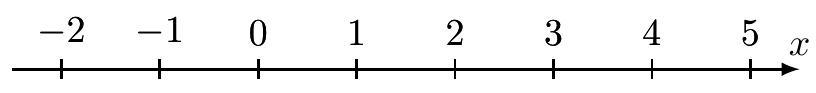
\includegraphics[max width=\textwidth, center]{2024_11_21_8f01584889ff06348ae7g-026}

UWAGA liczba 0 nie jest ani dodatnia, ani ujemna.\\
Zbiór liczb całkowitych matematycy oznaczają zazwyczaj literą \(\mathbb{Z}\). Czyli

\[
\mathbb{Z}=\{\ldots,-4,-3,-2,-1,0,1,2,3, \ldots\}
\]

Wobec tego prawdziwe są zdania \(2 \in \mathbb{N}, 2 \in \mathbb{Z},-2 \in \mathbb{Z}, \frac{1}{2} \notin \mathbb{Z}\).\\
Ponieważ każda liczba naturalna jest liczbą całkowitą, wobec tego zbiór liczb naturalnych jest podzbiorem zbioru liczb całkowitych, co zapisujemy \(\mathbb{N} \subset \mathbb{Z}\).

Liczba przeciwna do \(a\) jest to taka liczba, która w sumie z liczbą \(a\) daje 0 .

Liczbą przeciwną do 2 jest -2 , bo \(2+(-2)=0\).\\
Liczbą przeciwną do -3 jest \(-(-3)\) czyli liczba 3 , bo \(-3+3=0\).\\
Liczbą przeciwną do 0 jest liczba 0.\\
Ogólnie liczbę przeciwną do jakiejś liczby \(a\) oznaczamy (zazwyczaj) - \(a\).\\
Suma liczb całkowitych jest liczbą całkowitą, podobnie iloczyn liczb całkowitych jest liczbą całkowitą. Działania dodawania i mnożenia liczb całkowitych są przemienne i łączne.\\
Dodawanie liczby przeciwnej nazywamy odejmowaniem i wówczas zamiast pisać np.

\[
5+(-2) \quad \text { piszemy zazwyczaj } \quad 5-2
\]

Ogólnie:\\
jeżeli \(a, b\) są dowolnymi liczbami, to \(\quad a-b=a+(-b)\).\\
17. Wykonaj w pamięci poniższe odejmowania (dodawania)\\
а) \(14+(-5)=\)\\
b) \(15+(-9)=\)\\
c) \(-7+(-8)=\)\\
d) \(123-(-24)=\)\\
e) \(350-48=\)\\
f) \(460-64=\)\\
18. Wykonaj w pamięci poniższe odejmowania. Pamiętaj o tym, że wpierw musisz wykonać działanie w nawiasie.\\
a) \(22-(2-2)=\)\\
b) \((22-2)-2=\)\\
c) \((24-2)-6=\)\\
d) \(24-(2-6)=\)\\
e) \((12-6)-6=\)\\
f) \(12-(6-6)=\)\\
g) \(20-(8-6)=\)\\
h) \((20-8)-6=\)\\
i) \((5-3)-4=\)\\
j) \(5-(3-4)=\)\\
k) \((60-15)-5=\)\\
l) \(60-(15-5)=\)

UMOWA Ponieważ działanie odejmowania nie jest łączne, co widać w powyższym ćwiczeniu np. w podpunktach a) i b), dlatego musimy się umówić co wobec tego oznacza napis \(14-2-5\). Otóż, w powszechnie przyjętej umowie, \(14-2-5=(14-2)-5\).\\
Działanie mnożenia jest rozdzielne względem dodawania (odejmowania), oznacza to, że jeżeli \(a, b, c\) są dowolnymi liczbami, to

\[
\begin{aligned}
& \underbrace{a \cdot b+a \cdot c}_{\text {suma }}=\underbrace{a \cdot(b+c)}_{\text {iloczyn }} \\
& \underbrace{a \cdot b-a \cdot c}_{\text {różnica }}=\underbrace{a \cdot(b-c)}_{\text {iloczyn }}
\end{aligned}
\]

Ma miejsce następujący fakt, z którego w przyszłości będziemy wielokrotnie korzystać

\[
(-1) \cdot a=-a
\]

\section*{UZASADNIENIE}
Zauważ, że niezależnie od tego jaką liczbą jest \(a\) prawdziwe są poniższe równości

\[
0=0 \cdot a=\underbrace{(1+(-1))}_{=0} \cdot a=1 \cdot a+(-1) \cdot a=a+(-1) a .
\]

Z tego wynika, że

\[
0=a+(-1) a
\]

czyli

\[
(-1) a=-a
\]

\section*{PRZYKŁADY}
\[
\begin{aligned}
(-1) \cdot 1 & =-1 & (-1) \cdot(-4)=-(-4)=4 \\
(-1) \cdot 3 & =-3 & (-2) \cdot(-5)=(-1) \cdot 2 \cdot(-1) \cdot 5=1 \cdot 10=10 \\
(-1) \cdot(-1) & =-(-1)=1 & (-3) \cdot 7=(-1) \cdot 3 \cdot 7=(-1) \cdot 21=-21
\end{aligned}
\]

\section*{PRZYKŁAD}
\[
\begin{aligned}
3 \cdot(-7)-(-3) \cdot 5 & =-21-(-15) \\
& =-21+15 \\
& =-6
\end{aligned}
\]

\begin{enumerate}
  \setcounter{enumi}{18}
  \item Wykonaj następujące działania:\\
a) \((-2) \cdot(-4)+4 \cdot 3=\)\\
b) \(2 \cdot(-8)-2 \cdot(-3)=\)\\
c) \(-3 \cdot(3-8)-(-6) \cdot(-2)=\)\\
d) \((-1) \cdot(-2) \cdot(-5)+(-3) \cdot(-7)=\)\\
e) \((-4) \cdot(-2) \cdot(-1)-(-5) \cdot 3=\)\\
f) \(4 \cdot(-7)+(-1) \cdot(-3) \cdot(-5)=\)\\
g) \((-4) \cdot(-3) \cdot(-2) \cdot(-1)-(-2) \cdot 13=\)\\
h) \((-5) \cdot(-3) \cdot(-1) \cdot 1 \cdot 3 \cdot 5=\)
\end{enumerate}

\section*{ZAMIANA SUMY NA ILOCZYN}
PRZYKŁADY zamiany sumy na iloczyn.

\[
\begin{aligned}
& 17 \cdot 7+13 \cdot 7=(17+13) \cdot 7=30 \cdot 7=210 \\
& 19 \cdot 20+20=19 \cdot 20+1 \cdot 20=20 \cdot 20=400 \\
& 15+6 \boldsymbol{\uparrow}=21 \boldsymbol{n}
\end{aligned}
\]

\begin{enumerate}
  \setcounter{enumi}{19}
  \item Zapisz w podobny sposób w postaci iloczynu następujące sumy i tam gdzie można wykonaj w pamięci finalne mnożenie.\\
a) \(25 \cdot 13+75 \cdot 13=\)\\
b) \(399 \cdot 400+400=\)\\
c) \(12 \cdot 15+8 \cdot 15=\)\\
d) \(9 \cdot 4+16 \cdot 9=\)\\
e) \(17 \cdot 16+16 \cdot 13=\)\\
f) \(11 \cdot 14+19 \cdot 14=\)\\
g) \(27 \cdot 14+14 \cdot 73=\)\\
h) \(21 \cdot 24+79 \cdot 24=\)\\
i) \(9 \cdot 12+9 \cdot 18=\)\\
j) \(13 \cdot 67+13 \cdot 33=\)\\
k) \(14 \cdot 19+81 \cdot 14=\)\\
l) \(5 \cdot 17+83 \cdot 5=\)\\
m) \(3 \cdot \triangle+8 \cdot \triangle=\)\\
n) \(12 \square+11 \square=\)
\end{enumerate}

\section*{ZAMIANA ILOCZYNU NA SUME}
PRZYKŁADY zamiany iloczynu na sumę takich samych składników

\[
\begin{aligned}
& 3 \cdot 6=6+6+6=3+3+3+3+3+3 \\
& 5 \cdot 2=2+2+2+2+2=5+5 \\
& 3 \cdot 4=3+3+3+3=4+4+4
\end{aligned}
\]

\begin{enumerate}
  \setcounter{enumi}{20}
  \item Zapisz w postaci sumy, co najmniej dwóch, takich samych składników\\
a) \(241 \cdot 3\)\\
b) \(107 \cdot 5\)\\
c) \(71 \cdot 4\)\\
d) \(17 \cdot 5\)\\
e) \(9 \cdot 5\)\\
f) \(7 \cdot 3\)\\
g) \(5 \cdot 18\)\\
h) \(7 \cdot 23\)\\
i) \(19 \cdot 4\)\\
j) \(7 \cdot 5\)
\end{enumerate}

\section*{POTĘGI. KOLEJNOŚĆ WYKONYWANIA DZIAŁAŃ.}
Przypomnijmy wpierw i zapiszmy bardziej formalnie pojęcie potęgi:

\[
\begin{aligned}
& x^{n}=\underbrace{x \cdot x \cdot \ldots \cdot x}_{n \text { czynników }} \\
& x^{1}=x
\end{aligned}
\]

gdzie \(x\) nazywamy podstawą potęgi, zaś \(n\) wykładnikiem potęgi. Czyli potęga jest to zapisany w pewien sposób iloczyn takich samych czynników. Przy czym \(a^{2}\) nazywamy zazwyczaj kwadratem liczby a, zaś \(a^{3}-\) sześcianem liczby a.\\
22. Nie korzystając z kalkulatora wyznacz kwadraty wszystkich liczb naturalnych od 1 do 31.\\
23. Nie korzystając z kalkulatora wyznacz sześciany wszystkich liczb naturalnych od 1 do 10.\\
24. Nie korzystając z kalkulatora wyznacz\\
a) \(1^{4}, 2^{4}, \ldots, 5^{4}\)\\
b) \(2^{1}, 2^{2}, \ldots, 2^{10}\)\\
c) \(3^{1}, 3^{2}, \ldots, 3^{5}\)\\
d) \(5^{1}, 5^{2}, \ldots, 5^{5}\)

UWAGA Dobrze jest mieć osadzone w świadomości wyniki pierwszych dwóch zadań!\\
25. Wykonaj poniższe dzielenia przestrzegając kolejności wykonywania działań wyznaczonej przez nawiasy\\
a) \(24:(6: 2)\)\\
b) \((24: 6): 2\)\\
c) \((144: 3): 3\)\\
d) \(144:(3: 3)\)

Zauważ, że dzielenie, w przeciwieństwie do mnożenia, nie jest działaniem łącznym. Oznacza to, że nie możemy opuszczać nawiasów. W związku z tym, gdy spotykamy się z napisem \(18: 6: 3\), to musimy się umówić jak to rozumiemy. W powszechnie przyjętej umowie \(18: 6: 3=(18: 6): 3\).

\section*{UMOWA}
Aby uniknąć konieczności pisania dużej ilości nawiasów w matematyce przyjęta jest bardzo powszechnie umowa o kolejności wykonywania działań, z którą spotkałeś się w szkole podstawowej. Mówi ona, że wpierw wykonujemy działania w nawiasach, w następnej kolejności potęgowanie, potem mnożenie i dzielenie, a w końcu dodawanie i odejmowanie. Można ją streścić krótko:\\
wpierw potęgowanie, następnie mnożenie (dzielenie), a na końcu dodawanie (odejmowanie).

Dodatkowo, z uwagi na to, że odejmowanie i dzielenie nie jest łączne, w wyrażeniach arytmetycznych w których występuje dodawanie i odejmowanie, umawiamy się że działania te wykonujemy w kolejności od lewej do prawej. Analogicznie postępujemy, gdy mamy do czynienia z mnożeniem i dzieleniem.\\
Jeśli jednak zamiast odejmować będziemy dodawać liczbę przeciwną, a zamiast dzielić będziemy mnożyć przez liczbę odwrotną, to nie będzie problemu kolejności wykonywania działań, bowiem i dodawanie, i mnożenie jest działaniem łącznym.

\section*{PRZYKŁADY}
\[
\begin{aligned}
15-3 \cdot 4 & =15-12=3 \\
(-2) \cdot 5^{2} & =(-2) \cdot 25=-50 \\
0-5^{2} & =0-25=-25 \\
7-5^{2} & =7-25=-18 \\
-7^{2} & =-49 \\
-3^{2} \cdot 4 & =(-1) \cdot 3^{2} \cdot 4=(-1) \cdot 9 \cdot 4=-36
\end{aligned}
\]

\[
\begin{aligned}
(-3)^{2} \cdot 4 & =9 \cdot 4=36 \\
-5^{2} \cdot 4 & =(-1) \cdot 5^{2} \cdot 4=(-1) \cdot 25 \cdot 4=-100 \\
-7 \cdot 3^{2} & =-7 \cdot 9=-63 \\
\underbrace{(-2) \cdot 7}_{-14}-\underbrace{(-4) \cdot(-13)}_{52} & =-14-52=-66 \\
\underbrace{-5 \cdot 3}_{-15}-\underbrace{(-4) \cdot 7}_{-28} & =-15-(-28)=-15+28=13
\end{aligned}
\]

\begin{enumerate}
  \setcounter{enumi}{25}
  \item Zapisz poniższe wyrażenia w postaci jednej liczby\\
a) \((-2) \cdot(-5)+4=\)\\
b) \(-8-(-12):(-4)=\)\\
c) \(10-(-8):(-2)=\)\\
d) \((-4) \cdot(-3)-12=\)\\
e) \((-3) \cdot(-5)-(-15)=\)\\
f) \(-8-4 \cdot(-3)=\)\\
g) \(3 \cdot(-5)+6 \cdot(-2)=\)\\
h) \(5 \cdot(-2)-[(-2) \cdot 4]=\)\\
i) \((8-3) \cdot(-4)=\)\\
j) \(-7 \cdot(-4-3)=\)\\
k) \((-7-15):(-11)=\)\\
l) \(-7-(-3) \cdot(-11)=\)\\
m) \((-2) \cdot 7-4 \cdot(-4)=\)\\
n) \(3 \cdot(-5)-(-2) \cdot 4=\)
  \item Zapisz poniższe wyrażenia w postaci jednej liczby\\
a) \(3 \cdot 5^{2}=\)\\
b) \(2^{2} \cdot 3 \cdot 5^{2}=\)\\
c) \(4^{2} \cdot 5 \cdot 3^{2}=\)\\
d) \(2^{2} \cdot 7 \cdot 3^{2}=\)\\
e) \(9+2^{2} \cdot 3=\)\\
f) \(15+3 \cdot 5^{2}=\)\\
g) \(12-3^{2}=\)\\
h) \((-7)^{2}-4^{2}=\)\\
i) \(3 \cdot 7-5^{2}=\)\\
j) \(5^{2}-2 \cdot 6=\)\\
k) \(30-5 \cdot 3^{2}=\)\\
l) \(-5^{2}-(-6)^{2}=\)\\
m) \(70-2 \cdot 5^{2}=\)\\
n) \(-5^{2}-2 \cdot 7^{2}=\)\\
o) \(222-3 \cdot 9^{2}=\)
  \item Zapisz poniższe wyrażenia w postaci jednej liczby\\
a) \((-2)^{2}-8=\)\\
b) \(-5-\left(-2^{4}\right) \cdot 3=\)\\
c) \((-7)^{2} \cdot 2-(-3)^{2} \cdot 6=\)\\
d) \(-5-2^{4} \cdot 3=\)\\
e) \(-5+(-2)^{4} \cdot 3=\)\\
f) \(5+(-3) \cdot(-2)^{4}=\)\\
g) \(5-2^{4} \cdot 3=\)\\
h) \(5-(-2)^{4} \cdot 3=\)\\
i) \(-5^{2} \cdot 3-(-2)^{2} \cdot 7=\)\\
j) \(-2^{2}-8=\)\\
k) \(5-(-3) \cdot(-2)^{4}=\)\\
l) \(12-(-3)^{2} \cdot(-2)^{3}=\)\\
m) \(5-3 \cdot(-2)^{4}=\)\\
n) \(-(-2)^{2}-8=\)\\
о) \(-7^{2} \cdot 2-3^{2} \cdot(-2)=\)
\end{enumerate}

\subsection*{2.3 Liczby wymierne}
Liczby, które można przedstawić jako iloraz dwóch liczb całkowitych \(\frac{a}{b}\), nazywamy liczbami wymiernymi. Zbiór wszystkich liczb wymiernych matematycy oznaczają \(\mathbb{Q}\). Liczby te zapisujemy na jeden z dwóch sposobów:

\begin{enumerate}
  \item w postaci ułamka właściwego lub niewłaściwego,
  \item w postaci rozwinięcia dziesiętnego skończonego lub nieskończonego okresowego.\\
Wyrażenie \(\frac{a}{b}\) nazywamy ułamkiem. Jeżeli \(a<b\), to ułamek nazywamy ułamkiem właściwym, jeżeli \(a \geqslant b\), to ułamek nazywamy ułamkiem niewłaściwym. Przy czym jeżeli \(a=b\), to ułamek przedstawia liczbę 1. Gdy \(a\) jest wielokrotnością liczby \(b\), to ułamek \(\frac{a}{b}\) przedstawia liczbę całkowitą.\\
Jeżeli ułamek niewłaściwy \(\frac{a}{b}\) nie jest liczbą całkowitą, to zapisujemy go zazwyczaj w postaci tzw. liczby mieszanej.\\
PRZYKŁAD zamiany ułamka niewłaściwego na liczbę mieszaną.
\end{enumerate}

\[
\frac{17}{5}=\frac{15}{5}+\frac{2}{5}=3+\frac{2}{5}=3 \frac{2}{5}
\]

\begin{enumerate}
  \setcounter{enumi}{28}
  \item Zapisz w postaci liczby mieszanej, albo liczby całkowitej, każdy z poniższych ułamków niewłaściwych. Staraj się wszystkie obliczenia wykonywać w pamięci! Przyda ci się znajomość kwadratów liczb naturalnych.\\
a) \(\frac{18}{7}=\)\\
b) \(-\frac{16}{3}=\)\\
c) \(-\frac{37}{11}=\)\\
d) \(\frac{144}{11}=\)\\
e) \(\frac{160}{15}=\)\\
f) \(-\frac{289}{17}=\)\\
g) \(-\frac{300}{13}=\)\\
h) \(\frac{160}{8}=\)\\
i) \(-\frac{361}{19}=\)\\
j) \(-\frac{324}{9}=\)\\
k) \(-\frac{324}{18}=\)
\end{enumerate}

\begin{enumerate}
  \item \(\frac{441}{7}=\)
\end{enumerate}

Każdy ułamek właściwy można przedstawić na nieskończenie wiele sposobów w postaci ilorazu dwóch liczb całkowitych, a tylko w jeden sposób jako ułamek nieskracalny.\\
PRZYKŁAD rozszerzania ułamka:

\[
\frac{3}{7}=\frac{6}{14}=\frac{9}{21}=\ldots
\]

PRZYKŁAD upraszczania ułamka:

\[
\frac{54}{8 \cdot 18}=\frac{2 \cdot 3 \cdot 9}{8 \cdot 2 \cdot 9}=\frac{2 \cdot 3 \cdot 9}{2 \cdot 8 \cdot 9}=\frac{2}{2} \cdot \frac{3}{8} \cdot \frac{9}{9}=\frac{3}{8}
\]

\begin{enumerate}
  \setcounter{enumi}{29}
  \item Uprość w podobny sposób ułamki. Rozkładaj liczby na czynniki (niekoniecznie pierwsze), ale staraj się nie przekreślać liczb w trakcie upraszczania.\\
a) \(\frac{32 \cdot 3}{48}\)\\
b) \(\frac{3 \cdot 4}{10 \cdot 9}\)\\
c) \(\frac{15 \cdot 14}{21 \cdot 18}\)\\
d) \(\frac{6 \cdot 5 \cdot 2}{25 \cdot 12}\)\\
e) \(\frac{8 \cdot 27}{9 \cdot 32}\)\\
f) \(\frac{24 \cdot 15}{16 \cdot 9}\)\\
g) \(\frac{28 \cdot 35}{40 \cdot 49}\)\\
h) \(\frac{7 \cdot 24 \cdot 3}{18 \cdot 28 \cdot 6}\)\\
i) \(\frac{53 \cdot 27-27 \cdot 13}{72 \cdot 48-72 \cdot 28}\)\\
j) \(\frac{45 \cdot 22-5 \cdot 22}{121 \cdot 58-121 \cdot 8}\)\\
k) \(\frac{72 \cdot 35-35 \cdot 12}{14 \cdot 40-15 \cdot 14}\)
\end{enumerate}

\begin{enumerate}
  \item \(\frac{42 \cdot 15+15 \cdot 8}{29 \cdot 60-60 \cdot 14}\)\\
m) \(\frac{35 \cdot 6}{6+9}\)\\
n) \(\frac{40 \cdot 12}{5+9}\)\\
о) \(\frac{4+21}{8 \cdot 5}\)\\
p) \(\frac{15+10}{15-10}\)\\
q) \(\frac{9-2}{9+5}\)\\
r) \(\frac{17+18}{16+9}\)\\
s) \(\frac{10+25}{2+5}\)\\
t) \(\frac{15 \cdot 8}{5+4}\)\\
u) \(\frac{39+6}{13+2}\)\\
v) \(\frac{22+3}{5 \cdot 6}\)\\
w) \(\frac{15+10}{7 \cdot 5}\)
\end{enumerate}

\section*{PRZYKŁAD}
Sprowadź ułamki \(\frac{7}{26}, \frac{10}{39}, \frac{19}{78}\) do wspólnego mianownika i uporządkuj je rosnąco.\\
Te trzy liczby (ułamki) możemy przekształcić następująco, robimy to przy tym kolumnami:

\[
\begin{aligned}
\frac{7}{26} & =\frac{7}{2 \cdot 13}=\frac{3 \cdot 7}{3 \cdot 2 \cdot 13} \\
\frac{10}{39} & =\frac{10}{38} \\
\frac{19}{78} & =\frac{10 \cdot 2}{2 \cdot 3 \cdot 13} \\
\frac{19}{6 \cdot 13} & =\frac{20}{78} \\
& =\frac{19}{78}
\end{aligned}
\]

Zatem wyjściowe trzy liczby zapisane w porządku rosnącym to \(\frac{19}{78}, \frac{10}{39}, \frac{7}{26}\).\\
31. Sprowadź poniższe ułamki do wspólnego mianownika a następnie każdą trójkę liczb zapisz w porządku rosnącym:\\
a) \(\frac{5}{9}, \frac{19}{54}, \frac{13}{27}\)\\
b) \(\frac{11}{30}, \frac{4}{15}, \frac{3}{10}\)\\
c) \(\frac{5}{24}, \frac{3}{8}, \frac{11}{72}\)\\
d) \(\frac{35}{68}, \frac{9}{17}, \frac{19}{34}\)\\
е) \(\frac{5}{91}, \frac{3}{13}, \frac{1}{7}\)\\
32. Podaj po trzy przykłady liczby \(x\), która spełnia warunek:\\
a) \(\frac{3}{5}<x<\frac{4}{5}\)\\
b) \(\frac{1}{7}<x<\frac{2}{7}\)\\
c) \(\frac{1}{3}<x<\frac{2}{5}\)\\
d) \(\frac{2}{3}<x<\frac{3}{4}\)

PRZYKŁADY dodawania dwóch liczb mieszanych:

\[
\begin{aligned}
4 \frac{5}{7}+3 \frac{4}{7} & =4+3+\frac{5}{7}+\frac{4}{7}=4+3+\frac{9}{7}=7+1+\frac{2}{7}=8 \frac{2}{7} \\
3 \frac{5}{7}+4 \frac{8}{9} & =3+4+\frac{5}{7}+\frac{8}{9}=7+\frac{45}{63}+\frac{56}{63}=7+\frac{101}{63}=7+1 \frac{38}{63}=8 \frac{38}{63} \\
4 \frac{5}{21}+5 \frac{8}{35} & =4+5+\frac{5}{3 \cdot 7}+\frac{8}{7 \cdot 5}=9+\frac{5 \cdot 5}{3 \cdot 7 \cdot 5}+\frac{8 \cdot 3}{5 \cdot 7 \cdot 3} \\
& =9+\frac{25}{105}+\frac{24}{105}=9 \frac{49}{105}
\end{aligned}
\]

\begin{enumerate}
  \setcounter{enumi}{32}
  \item Wykonaj poniższe dodawania. Wynik zapisz w postaci ułamka właściwego nieskracalnego albo też liczby mieszanej, w której część ułamkowa jest nieskracalna.\\
a) \(5 \frac{1}{7}+3 \frac{4}{70}=\)\\
b) \(\frac{11}{12}+\frac{5}{72}=\)\\
c) \(7 \frac{2}{77}+13 \frac{4}{11}=\)\\
d) \(2 \frac{5}{14}+7 \frac{5}{6}=\)\\
e) \(1 \frac{4}{15}+5 \frac{2}{55}=\)\\
f) \(4 \frac{11}{21}+3 \frac{22}{35}=\)\\
g) \(13 \frac{7}{15}+12 \frac{19}{45}=\)\\
h) \(\frac{17}{1205}+\frac{31}{2410}=\)\\
i) \(2012 \frac{7}{2012}+2011 \frac{5}{4024}=\)
\end{enumerate}

PRZYKŁADY odejmowania dwóch liczb mieszanych:

\[
\begin{aligned}
5 \frac{3}{8}-2 \frac{7}{8} & =4 \frac{11}{8}-2 \frac{7}{8}=2 \frac{4}{8}=2 \frac{1}{2} \\
4 \frac{8}{9}-3 \frac{5}{7} & =4+\frac{8}{9}-\left(3+\frac{5}{7}\right)=4-3+\frac{8}{9}-\frac{5}{7}=1+\frac{56-45}{63}=1 \frac{11}{63} \\
5 \frac{8}{35}-4 \frac{5}{21} & =5-4+\frac{8}{35}-\frac{5}{21}=1+\frac{24}{105}-\frac{25}{105}=1-\frac{1}{105}=\frac{104}{105}
\end{aligned}
\]

\begin{enumerate}
  \setcounter{enumi}{33}
  \item Wykonaj poniższe odejmowania. Wynik zapisz w postaci ułamka właściwego nieskracalnego albo też liczby mieszanej, w której część ułamkowa jest nieskracalna.\\
a) \(10-2 \frac{5}{7}=\)\\
b) \(77 \frac{13}{21}-26 \frac{20}{21}=\)\\
c) \(5 \frac{3}{7}-2 \frac{5}{7}=\)\\
d) \(34 \frac{25}{41}-13 \frac{38}{41}=\)\\
e) \(64 \frac{15}{32}-37 \frac{19}{32}=\)\\
f) \(6 \frac{3}{7}-\frac{4}{7}=\)\\
g) \(5 \frac{5}{12}-2 \frac{7}{12}=\)\\
h) \(3 \frac{15}{28}-1 \frac{5}{8}=\)\\
i) \(5 \frac{3}{22}-2 \frac{8}{33}=\)
  \item Wykonaj poniższe dodawania i odejmowania. Wynik zapisz w postaci ułamka właściwego nieskracalnego albo też liczby mieszanej.\\
a) \(2 \frac{1}{2}-\frac{3}{4}=\)\\
b) \(3 \frac{5}{9}-1 \frac{8}{15}=\)\\
c) \(3 \frac{1}{3}-\frac{4}{5}=\)\\
d) \(5 \frac{3}{5}+\frac{1}{3}=\)\\
e) \(12 \frac{9}{10}+15 \frac{3}{8}=\)\\
f) \(5 \frac{3}{8}-1 \frac{7}{10}=\)\\
g) \(9 \frac{11}{40}-7 \frac{18}{25}=\)\\
h) \(9 \frac{7}{8}-7 \frac{29}{36}=\)\\
i) \(8 \frac{17}{50}-4 \frac{37}{75}=\)
  \item Korzystając z łączności i przemienności dodawania oblicz w pamięci\\
a) \(\left(\frac{2}{5}+1 \frac{3}{7}\right)+\frac{4}{7}=\)\\
b) \(\frac{2}{13}+\left(11 \frac{11}{13}+1 \frac{13}{15}\right)=\)\\
c) \(\left(1 \frac{2}{3}+5 \frac{1}{2}\right)+1 \frac{1}{3}=\)\\
d) \(\left(\frac{2}{5}+\frac{4}{9}\right)+1 \frac{3}{5}=\)
\end{enumerate}

\section*{PRZYKŁADY}
\(3 \cdot \frac{5}{6}=\frac{3 \cdot 5}{6}=\frac{3 \cdot 5}{3 \cdot 2}=\frac{5}{2}\)\\
\(\frac{7}{12} \cdot \frac{3}{14}=\frac{7 \cdot 3}{12 \cdot 14}=\frac{7 \cdot 3}{3 \cdot 4 \cdot 2 \cdot 7}=\frac{7 \cdot 3}{7 \cdot 3} \cdot \frac{1}{4 \cdot 2}=\frac{1}{8}\)\\
\(15 \cdot 4 \frac{2}{7}=15 \cdot \frac{30}{7}=\frac{15 \cdot 30}{7}=\frac{450}{7}=64 \frac{2}{3}\)\\
\(7 \frac{1}{3} \cdot 8 \frac{2}{3}=\frac{22}{3} \cdot \frac{26}{3}=\frac{572}{9}=63 \frac{5}{9}\)\\
37. Wykonaj poniższe mnożenia. Odpowiedzi zapisuj w postaci liczb całkowitych albo też liczb mieszanych, w których część ułamkowa jest ułamkiem nieskracalnym.\\
a) \(2 \cdot \frac{5}{6}=\)\\
b) \(24 \cdot \frac{7}{72}=\)\\
c) \(6 \frac{1}{4} \cdot 6=\)\\
d) \(9 \cdot 7 \frac{2}{3}=\)\\
e) \(16 \cdot 4 \frac{3}{4}=\)\\
f) \(8 \frac{3}{5} \cdot 15=\)\\
g) \(2 \frac{2}{3} \cdot 1 \frac{4}{5}=\)\\
h) \(3 \frac{3}{5} \cdot 1 \frac{1}{9}=\)\\
i) \(4 \frac{2}{7} \cdot 3 \frac{4}{15}=\)\\
38. Wykonaj poniższe mnożenia. Odpowiedzi zapisuj w postaci liczb całkowitych albo też liczb mieszanych, w których część ułamkowa jest ułamkiem nieskracalnym.\\
a) \(\frac{16}{17} \cdot \frac{51}{64}=\)\\
b) \(\frac{11}{15} \cdot \frac{25}{44}=\)\\
c) \(\frac{24}{35} \cdot \frac{55}{84}=\)\\
d) \(2 \frac{3}{4} \cdot 1 \frac{2}{3}=\)\\
e) \(7 \frac{1}{8} \cdot 11 \frac{1}{3}=\)\\
f) \(4 \frac{4}{5} \cdot 4 \frac{2}{7}=\)

\section*{FAKT}
Każda liczba wymierna (z wyjątkiem 0) ma tzw liczbę odwrotną. Liczbą odwrotną do liczby \(\frac{a}{b}\) jest liczba \(\frac{b}{a}\). Iloczyn liczby wymiernej i liczby do niej odwrotnej jest równy 1.\\
39. Wyznacz odwrotności następujących liczb. Odpowiedzi zapisuj w postaci ułamka właściwego, liczby całkowitej albo też liczby mieszanej.\\
а) \(\frac{4}{7}\)\\
b) \(\frac{5}{11}\)\\
c) \(\frac{1}{3}\)\\
d) \(\frac{4}{15}\)\\
e) \(\frac{5}{13}\)\\
f) \(2 \frac{1}{3}\)\\
g) \(5 \frac{1}{7}\)\\
h) \(6 \frac{1}{6}\)\\
40. Wykonaj dzielenie poniższych par liczb. Wynik zapisz w postaci ułamka właściwego, a gdy wynik jest ułamkiem niewłaściwym to w postaci liczby całkowitej lub też liczby mieszanej\\
a) \(1: \frac{1}{7}\)\\
b) \(3: \frac{1}{4}\)\\
c) \(7: \frac{1}{7}\)\\
d) \(7: \frac{4}{5}\)\\
е) \(8: \frac{7}{9}\)\\
f) \(\frac{1}{3}: \frac{1}{6}\)\\
g) \(\frac{1}{8}: \frac{1}{3}\)\\
h) \(\frac{1}{4}: \frac{5}{8}\)\\
i) \(16: \frac{6}{7}\)\\
j) \(121: \frac{11}{12}\)\\
k) \(98: 1 \frac{2}{5}\)

\begin{enumerate}
  \item \(\frac{5}{9}: \frac{7}{18}\)\\
m) \(1 \frac{3}{5}: \frac{2}{15}\)\\
n) \(6 \frac{2}{7}: \frac{4}{21}\)\\
о) \(13 \frac{1}{5}: \frac{11}{16}\)\\
p) \(\frac{24}{25}: 3 \frac{1}{5}\).
\end{enumerate}

\begin{enumerate}
  \setcounter{enumi}{40}
  \item Uzupełnij poniższą tabelkę
\end{enumerate}

\begin{center}
\begin{tabular}{|l|c|c|c|c|c|c|c|c|c|}
\hline
 & a) & b) & c) & d) & e) & f) & g) & h) & i) \\
\hline
liczba \(a\) & 3 & \(1 \frac{1}{5}\) & \(-1 \frac{1}{2}\) &  &  &  &  &  &  \\
\hline
przeciwna do \(a\) &  &  &  & -3 & \(1 \frac{1}{4}\) & \(\frac{2}{3}\) &  &  &  \\
\hline
odwrotna do \(a\) &  &  &  &  &  &  & \(\frac{1}{2}\) & \(-\frac{2}{3}\) & \(1 \frac{1}{5}\) \\
\hline
\end{tabular}
\end{center}

\section*{PRZYKŁAD}
Na początku roku w szkole było 285 uczniów, przy czym 13/19 liczby uczniów stanowili chłopcy. W ciągu roku szkolnego liczba uczniów zwiększyła się o \(5 / 19\), przy czym \(1 / 3\) liczby osób, które doszły, to były dziewczyny. Ilu chłopców było w szkole na koniec roku szkolnego?

\section*{Rozwiązanie}
Liczba chłopców na koniec roku szkolnego

\[
\frac{13}{19} \cdot 285=13 \cdot \frac{285}{19}=13 \cdot 15=150+45=195
\]

Liczba uczniów, którzy doszli do szkoły w ciągu roku szkolnego

\[
\frac{5}{19} \cdot 285=5 \cdot \frac{285}{19}=5 \cdot 15=75
\]

Liczba dziewczyn, które doszły w ciągu roku szkolnego

\[
\frac{1}{3} \cdot 75=25
\]

zatem chłopców doszło \(75-25=50\). Stąd liczba chłopców na koniec roku szkolnego

\[
195+50=245
\]

\begin{enumerate}
  \setcounter{enumi}{41}
  \item W naszej szkole jest 420 uczniów. Tramwajem dojeżdża do szkoły \(2 / 5\) wszystkich uczniów, autobusem - 13/105, samochodem \(-1 / 7\). Pozostali uczniowie chodzą do szkoły pieszo. Ilu uczniów chodzi do szkoły pieszo?
  \item W szkole uczy się 1440 uczniów. Dwie trzecie z nich wyjechało na wakacje nad morze. Dwie trzecie z pozostałych uczniów wyjechało na wakacje w góry, zaś jedna czwarta z tych, którzy nie wyjechali ani w góry ani nad morze wyjechała na biwaki nad jezioro. Pozostali uczniowie nigdzie nie wyjechali. Ilu było takich uczniów?
  \item W naszej klasie jest 25 osób i średnia waga ucznia w naszej klasie wynosi 56 kilogramów. W sąsiedniej klasie jest 30 uczniów i średnia waga ucznia w tej drugiej klasie jest równa 51 kilogramów. Jaka jest średnia waga ucznia w tych dwóch klasach? Odpowiedź podaj w postaci liczby mieszanej.
  \item Średnia arytmetyczna trzech liczb jest równa \(12 \frac{1}{3}\). Najmniejsza z tych liczb jest równa 11 i jest o 3 mniejsza od największej. Jaka jest trzecia z tych liczb?
\end{enumerate}

\section*{ZAPIS DZIESIĘTNY LICZBY WYMIERNEJ}
\section*{OKREŚLENIE}
Ułamek dziesiętny jest to taki ułamek, którego mianownik jest równy 10 lub jest potęgą liczby 10.

\section*{PRZYKŁADY}
\[
\frac{3}{10}, \quad \frac{17}{100}, \quad \frac{15}{1000}, \quad \frac{26}{10}
\]

Zamiana ułamka nieskracalnego na ułamek dziesiętny polega na pomnożeniu licznika i mianownika przez odpowiednią, ale taką samą liczbę całkowitą, aby w wyniku tego mnożenia mianownik stał się liczbą 10 lub potęga liczby 10.\\
W tym celu zauważmy, że \(10=2 \cdot 5\). Jest to przedstawienie liczby 10 w postaci iloczynu liczb pierwszych. Ponieważ liczbę naturalną można tylko w jeden sposób przedstawić jako iloczyn liczb pierwszych, wobec tego ułamek nieskracalny można zamienić na dziesiętny tylko wówczas gdy jego mianownik w rozkładzie na czynniki pierwsze zawiera tylko 2-ki i 5-ki.

\section*{PRZYKŁADY}
\[
\begin{aligned}
& \frac{1}{2}=\frac{1}{2} \cdot \frac{5}{5}=\frac{5}{10} \\
& \frac{3}{4}=\frac{3}{2 \cdot 2}=\frac{3}{2 \cdot 2} \cdot \frac{5 \cdot 5}{5 \cdot 5}=\frac{3 \cdot 5 \cdot 5}{2 \cdot 5 \cdot 2 \cdot 5}=\frac{75}{10 \cdot 10}=\frac{75}{100} \\
& \frac{3}{5}=\frac{3}{5} \cdot \frac{2}{2}=\frac{6}{10} \\
& \frac{14}{25}=\frac{14 \cdot 2 \cdot 2}{25 \cdot 2 \cdot 2}=\frac{14 \cdot 4}{5 \cdot 2 \cdot 5 \cdot 2}=\frac{64}{100}
\end{aligned}
\]

\begin{enumerate}
  \setcounter{enumi}{45}
  \item Zamień poniższe ułamki zwykłe na dziesiętne rozszerzając odpowiednio licznik i mianownik każdego ułamka dokładnie tak jak w powyższych przykładach\\
a) \(\frac{1}{2}\)\\
b) \(\frac{3}{5}\)\\
c) \(\frac{3}{4}\)\\
d) \(\frac{1}{8}\)\\
e) \(\frac{7}{20}\)\\
f) \(\frac{24}{25}\)
\end{enumerate}

PRZYKŁADY wyjaśniające związek pomiędzy ułamkami dziesiętnymi a rozwinięciem dziesiętnym skończonym liczby wymiernej. Po lewej stronie znaku równości jest zapis dziesiętny liczby a po prawej suma odpowiadających jej ułamków dziesiętnych.

\[
\begin{aligned}
& 6,3=6+\frac{3}{10} \\
& 2,73=2+\frac{7}{10}+\frac{3}{100} \\
& 0,7023=\frac{7}{10}+\frac{0}{100}+\frac{2}{1000}+\frac{3}{10000}
\end{aligned}
\]

PRZYKŁAD rozszerzenia ułamka zwykłego do ułamka dziesiętnego

\[
\frac{8}{125}=\frac{8 \cdot 2}{125 \cdot 2}=\frac{16}{250}=\frac{16 \cdot 2}{250 \cdot 2}=\frac{32}{500}=\frac{64}{1000}=0,064
\]

\begin{enumerate}
  \setcounter{enumi}{46}
  \item Zamień poniższe ułamki zwykłe na dziesiętne rozszerzając odpowiednio licznik i mianownik każdego ułamka, a następnie podaj rozwinięcie dziesiętne każdej z tych liczb.\\
a) \(\frac{3}{20}\)\\
b) \(\frac{3}{125}\)\\
c) \(\frac{9}{40}\)\\
d) \(\frac{37}{200}\)\\
e) \(\frac{1}{32}\)\\
f) \(\frac{9}{500}\)\\
g) \(\frac{12}{15}\)\\
h) \(\frac{14}{35}\)\\
i) \(\frac{22}{110}\)\\
j) \(\frac{19}{50}\)\\
k) \(\frac{111}{500}\)
\end{enumerate}

\begin{enumerate}
  \item \(\frac{7}{8}\)
\end{enumerate}

\begin{enumerate}
  \setcounter{enumi}{47}
  \item Wyznacz rozwinięcie dziesiętne nieskończone okresowe poniższych liczb wymiernych, dzieląc pisemnie licznik przez mianownik.\\
a) \(\frac{4}{9}\)\\
b) \(\frac{3}{11}\)\\
c) \(\frac{8}{15}\)\\
d) \(\frac{5}{6}\)\\
e) \(\frac{5}{12}\)\\
f) \(\frac{1}{37}\)
\end{enumerate}

PRZYKŁAD zamiany liczby o podanym rozwinięciu dziesiętnym na ułamek zwykły.

\[
0,56=\frac{56}{100}=\frac{2 \cdot 28}{2 \cdot 50}=\frac{2 \cdot 2 \cdot 14}{2 \cdot 2 \cdot 25}=\frac{14}{25} \cdot \frac{2}{2} \cdot \frac{2}{2}=\frac{14}{25}
\]

\begin{enumerate}
  \setcounter{enumi}{48}
  \item Zamień liczby o podanych rozwinięciach dziesiętnych na ułamki zwykłe, podobnie jak w powyższym przykładzie, doprowadzając je do nieskracalnej postaci.\\
a) 0,5\\
b) 0,018\\
c) 0,125\\
d) 0,375\\
e) 0,32\\
f) 0,0625\\
g) 0,875\\
h) 0,024\\
i) 0,225\\
j) 0,185\\
k) 0,03125
  \item Oblicz, pamiętając o kolejności wykonywania działań oraz o tym, że kreska ułamkowa zastępuje znak dzielenia, a wyrażenia w liczniku i w mianowniku traktujemy tak jakby były w nawiasie.\\
Na przykład \(\frac{1+\frac{1}{3}}{3-\frac{1}{7}}=\left(1+\frac{1}{3}\right):\left(3-\frac{1}{7}\right)\)\\
a) \(\frac{5 \frac{1}{2}+2,8}{7+1,5: \frac{3}{8}}\)\\
b) \(\left(-2 \frac{3}{5}\right) \cdot\left(-6 \frac{1}{4}\right)-\left(-3 \frac{1}{4}\right):\left(-3 \frac{5}{7}\right)+\frac{5}{8}\)\\
c) \(4 \frac{4}{5}: 1,6 \cdot 1 \frac{7}{8}-1 \frac{5}{8}+2,25\)\\
d) \(16 \frac{2}{3}: 2 \frac{7}{9}: 3,6-1,6 \cdot 2 \frac{3}{4}: 5,5\)\\
е) \(\frac{\frac{5}{7}:\left(-1 \frac{5}{7}\right)}{-\left(3 \frac{1}{4}-5,5 \cdot \frac{1}{6}\right)+1,5}\)\\
f) \(\frac{\left[(-9)^{2} \cdot 2\right]:(-3)^{2}}{-(-8)+(-5) \cdot 4}: \frac{(-2) \cdot(-9)}{5-9}\)\\
g) \(\frac{4,4-\frac{2}{3} \cdot 1,8}{\frac{3}{8} \cdot 4^{2}-\frac{1}{4} \cdot 2^{3}}\)\\
h) \(\frac{-3^{2}+(-2)^{3}}{-2-(-3)}: \frac{(-4)^{2}-(-2)^{2}}{-4-(-1)}\)\\
i) \(\frac{\left(-2 \frac{1}{5}-0,2\right): 1 \frac{3}{5}}{-0,2 \cdot 0,3}\)\\
j) \(\left(-4 \frac{2}{3}\right) \cdot\left(-2 \frac{2}{7}\right)-3 \frac{1}{3} \cdot\left(0,8-2 \frac{1}{5}\right)^{2}\)\\
k) \(\frac{1}{1+\frac{1}{3}}: \frac{1+\frac{1}{2}}{1-\frac{1}{3}}\)\\
l) \(\left(1+\frac{\frac{1}{2}-1}{\frac{1}{2}+1}\right):\left(1-\frac{\frac{1}{2}+1}{\frac{1}{2}-1}\right)\)\\
m) \(1+\frac{1}{1+\frac{1}{2}}\)\\
n) \(1+\frac{1}{1+\frac{1}{1+\frac{1}{3}}}\)\\
o) \(2+\frac{2}{2+\frac{1}{2+\frac{1}{2+\frac{1}{2}}}}\)\\
p) \(\left(1-\frac{1}{1-\frac{1}{1-\frac{1}{3}}}\right)^{2}:\left(2-\frac{2}{2-\frac{1}{2-\frac{1}{2}}}\right)^{3}\)
\end{enumerate}

\subsection*{2.4 Notacja wykładnicza zapisu liczb}
W zastosowaniach matematyki, w szczególności w fizyce, chemii, astronomii mamy nie raz do czynienia z dużymi liczbami. Zapisywanie tych liczb w tradycyjnej notacji dziesiętnej czyni je trudnymi do odczytania. W takich sytuacjach stosuje się tzw. notację wykładnicza lub też jak mówią anglosasi notację naukowq. Ponieważ w notacji tej używa się potęg liczby 10 przedstawmy wpierw niektóre potęgi 10 i nazwy niektórych z tych liczb.

\[
\begin{aligned}
10^{1} & =10 \\
10^{3} & =1000 \\
10^{6} & =1000000 \quad \text { milion } \\
10^{9} & =1000000000 \quad \text { miliard } \quad \text { (ang. bilion) } \\
10^{12} & =1000000000000 \quad \text { bilion } \quad \text { (ang. trylion) } \\
10^{15} & =1000000000000000 \quad \text { (ang. kwadrylion) } \\
10^{18} & =1000000000000000000 \quad \text { trylion } \quad \text { (ang. pentylion) }
\end{aligned}
\]

Zanim zajmiemy się notacją wykładniczą zapoznajmy się wpierw z działaniami na potęgach liczby 10, bowiem działania na liczbach zapisanych w postaci wykładniczej sprowadzają się w dużej mierze do operowania na potęgach liczby 10.\\
MNOŻENIE, DZIELENIE I POTĘGOWANIE POTĘG LICZBY 10 PRZYKŁAD

\[
10^{3} \cdot 10^{5}=(10 \cdot 10 \cdot 10) \cdot(10 \cdot 10 \cdot 10 \cdot 10 \cdot 10)=10^{3+5}=10^{8}
\]

Ogólnie

\[
10^{m} \cdot 10^{n}=\underbrace{(10 \cdot 10 \cdot \ldots 10)}_{m \text { czynników }} \cdot \underbrace{(10 \cdot 10 \cdot \ldots 10)}_{n \text { czynników }}=10^{m+n} \quad m, n \in \mathbb{N}
\]

\begin{enumerate}
  \setcounter{enumi}{50}
  \item Wykonaj poniższe możenia zapisując wynik w postaci potęgi liczby 10.\\
a) \(10^{4} \cdot 10^{5}=\)\\
b) \(10 \cdot 10^{6}=\)\\
c) \(10^{2} \cdot 10^{4} \cdot 10^{5}=\)\\
d) \(2 \cdot 10^{4} \cdot 5 \cdot 10^{11}=\)\\
e) \(2,5 \cdot 10^{4} \cdot 4 \cdot 10^{13}=\)\\
f) \(50 \cdot 10^{3} \cdot 2 \cdot 10^{7}=\)\\
g) \(8 \cdot 10^{3} \cdot 125 \cdot 10^{2}=\)\\
h) \(25 \cdot 10^{5} \cdot 4 \cdot 10^{7}\)
\end{enumerate}

\section*{PRZYKŁADY}
\[
\begin{aligned}
& \frac{10^{5}}{10^{3}}=\frac{10 \cdot 10 \cdot 10 \cdot 10 \cdot 10}{10 \cdot 10 \cdot 10}=\underbrace{\frac{10 \cdot 10 \cdot 10}{10 \cdot 10 \cdot 10} \cdot 10 \cdot 10=10^{5-3}=10^{2}}_{=1} \\
& \frac{10^{4}}{10^{4}}=1 \\
& \frac{10^{3}}{10^{5}}=\frac{10 \cdot 10 \cdot 10}{10 \cdot 10 \cdot 10 \cdot 10 \cdot 10}=\underbrace{\frac{10 \cdot 10 \cdot 10}{10 \cdot 10 \cdot 10}}_{=1} \cdot \frac{1}{10 \cdot 10}=\frac{1}{10 \cdot 10}=\frac{1}{10^{5-3}}=\frac{1}{10^{2}}
\end{aligned}
\]

Ogólnie

\[
\frac{10^{m}}{10^{n}}= \begin{cases}10^{m-n} & \text { gdy } m>n \\ 1 & \text { gdy } m=n \\ \frac{1}{10^{n-m}} & \text { gdy } m<n\end{cases}
\]

\begin{enumerate}
  \setcounter{enumi}{51}
  \item Oblicz, zapisując wynik podobnie jak w powyższych przykładach.\\
a) \(\frac{10^{5}}{10^{2}}=\)\\
b) \(\frac{10^{7}}{10^{7}}=\)\\
c) \(\frac{2,5 \cdot 10^{10} \cdot 80 \cdot 10^{9}}{2 \cdot 10^{6}}=\)\\
d) \(\frac{10^{6}}{10}=\)\\
e) \(\frac{10}{10^{7}}=\)\\
f) \(\frac{125 \cdot 10^{6} \cdot 4 \cdot 10^{8}}{5 \cdot 10^{4}}=\)\\
g) \(\frac{10^{2}}{10^{9}}=\)\\
h) \(\frac{60 \cdot 10^{17}}{2 \cdot 10^{2} \cdot 3 \cdot 10^{5}}=\)\\
i) \(\frac{4 \cdot 10^{18} \cdot 50 \cdot 10^{6}}{2 \cdot 10^{9}}=\)
\end{enumerate}

\section*{POTĘGOWANIE POTĘG}
\section*{PRZYKŁAD}
\[
\left(10^{5}\right)^{3}=10^{5} \cdot 10^{5} \cdot 10^{5}=10^{5+5+5}=10^{3 \cdot 5}=10^{15}
\]

Ogólnie

\[
\left(10^{m}\right)^{n}=\underbrace{10^{m} \cdot \ldots \cdot 10^{m}}_{n \text { czynników }}=10^{m+m+\ldots+m} \overbrace{n \text { składników }}^{m+\ldots}=10^{m \cdot n}
\]

\begin{enumerate}
  \setcounter{enumi}{52}
  \item Wylicz, zapisując wynik w postaci potęgi liczby 10.\\
a) \(\left(10^{3} 0\right)^{2}=\)\\
b) \(\left(10^{2} 0\right)^{4}=\)\\
c) \(\left(10^{3} 0\right)^{3}=\)\\
d) \(\left(10^{5} 0\right)^{6}=\)\\
e) \(\left(10^{9} 0\right)^{11}=\)\\
f) \(\left(10^{4} 0\right)^{5}=\)
\end{enumerate}

\section*{POSTAĆ WYKŁADNICZA ZAPISU LICZB}
\section*{PRZYKŁAD}
W astronomii jako jednostkę długości wykorzystuje się rok świetlny czyli drogę jaką promień światła przebywa w ciągu jednego roku zwrotnikowego. Rok zwrotnikowy jest to 365,24 doby. Ponieważ prędkość światła jest równa \(299790 \mathrm{~km} / \mathrm{s}\), doba ma 24 godziny, godzina 60 minut, a minuta 60 sekund wobec tego

\[
\begin{aligned}
\text { 1rok świetlny } & =299790 \frac{\mathrm{~km}}{\mathrm{~s}} \cdot 365,24 \cdot 24 \cdot 60 \cdot 60 \mathrm{~s} \\
& \approx 9460000000000000 \mathrm{~km} \\
& =9460000000000000000 \mathrm{~m}
\end{aligned}
\]

Tak duża liczba nie jest od razu łatwa do ocenienia jak i do przeczytania. Z tego względu takie liczby zamiast pisać w postaci dziesiętnej przedstawia się w tzw. postaci wykładniczej czyli w postaci iloczynu dwóch liczb: jedna z nich jest liczbą pomiędzy 1 i 10, a druga liczba jest potęgą 10. Mamy zatem

\[
\text { 1rok świetlny } \approx 9,46 \cdot 1000000000000000000 \mathrm{~m}=9,46 \cdot 10^{18} \mathrm{~m}
\]

Ten sposób zapisywania liczb nazywamy postacią wykładniczą (ang. scientific notation). Ogólna postać zapisywania liczb w tej notacji, to

\[
a \cdot 10^{n}, \quad \text { gdzie } \quad 1 \leqslant a<10, n \in \mathbb{N}_{+}
\]

przy czym czynnik \(a\) nazywamy mantysą liczby.\\
Wyliczona w powyższym przykładzie wartość roku świetlnego w metrach jest tylko wielkością przybliżoną. Faktycznie tylko pierwsze cztery cyfry 9460 są dokładne. Jeżeli liczba zapisana w postaci wykładniczej jest wynikiem jakiegoś pomiaru, to zazwyczaj jest ona obarczona jakimś błędem. Powszechna umowa jest taka: w mantysie zapisujemy tylko te cyfry, które są dokładne. Przy takiej umowie zamiast używać znaku \(\approx\) używamy znaku równości \(=\).\\
Na przykład:

\[
1 \text { rok świetlny }=9,460 \cdot 10^{18} \mathrm{~m}
\]

rozumiejąc przez to, że w zapisie liczby 9,460 wszystkie cyfry są dokładne.\\
54. Zapisz poniższe liczby w postaci wykładniczej:\\
a) \(50000=\)\\
b) \(2500=\)\\
c) \(25=\)\\
d) \(123456=\)\\
e) \(12,3456=\)\\
f) \(123,456=\)\\
g) \(20000=\)\\
h) \(230032=\)\\
i) \(2010,0102=\)\\
55. Zapisz w postaci dziesiętnej:\\
a) \(2 \cdot 10^{4}=\)\\
b) \(5 \cdot 10^{6}=\)\\
c) \(2,5 \cdot 10^{7}=\)\\
d) \(3,45 \cdot 10^{4}=\)\\
e) \(3,112 \cdot 10^{6}=\)\\
f) \(3,02 \cdot 10^{5}=\)\\
g) \(3,20 \cdot 10^{4}=\)\\
h) \(75 \cdot 10^{2}=\)\\
i) \(0,75 \cdot 10^{4}=\)

Liczby mające większą ilość cyfr różnych od zera, zapisując w postaci wykładniczej, zaokrąglamy do mniejszej ilości cyfr. Na przykład w jakimś państwie pewnego dnia zarejestrowanych było 30784235 samochodów. Ta liczba zapisana w postaci wykładniczej z mantysą zaokrągloną do 2 cyfr ma postać \(3,1 \cdot 10^{7}\), bowiem \(30784235 \approx 31000000=3,1 \cdot 10^{7}\)\\
56. W poniższym ćwiczeniu zapisz każdą z liczb w postaci wykładniczej, zaokrąglając mantysę do 2 cyfr po przecinku.\\
(a) Powierzchnia kuli ziemskiej \(P=510101000 \mathrm{~km}^{2}\)\\
(b) Objętość kuli ziemskiej \(V=1083319780000 \mathrm{~km}^{3}\)\\
(c) Prędkość światła \(c=299792458 \mathrm{~m} / \mathrm{s}\)\\
(d) Liczba sekund w jednej dobie.\\
(e) Liczba sekund w 1 roku kalendarzowym, czyli w 365 dniach.

MNOŻENIE, DZIELENIE I POTĘGOWANIE LICZB ZAPISANYCH W POSTACI WYKŁADNICZEJ

\section*{PRZYKEADY}
\[
\begin{aligned}
2,4 \cdot 10^{5} \cdot 5 \cdot 10^{3} & =12 \cdot 10^{5+3}=1,2 \cdot 10 \cdot 10^{8}=1,2 \cdot 10^{9} \\
15 \cdot 10^{8} \cdot 8 \cdot 10^{7} & =120 \cdot 10^{15}=1,2 \cdot 10^{2} \cdot 10^{15}=1,2 \cdot 10^{17}
\end{aligned}
\]

\begin{enumerate}
  \setcounter{enumi}{56}
  \item Wykonaj możenie liczb zapisując wynik w postaci wykładniczej\\
a) \(3 \cdot 10^{2} \cdot 10^{4} \cdot 11 \cdot 10^{5}=\)\\
b) \(4 \cdot 10^{2} \cdot 10^{5}=\)\\
c) \(2 \cdot 10^{3} \cdot 3 \cdot 10^{5}=\)\\
d) \(4 \cdot 10^{4} \cdot 7 \cdot 10^{5}=\)\\
e) \(2,2 \cdot 10^{4} \cdot 5 \cdot 10^{11}=\)\\
f) \(7 \cdot 10^{5} \cdot 8 \cdot 10^{12}=\)\\
g) \(2,7 \cdot 10^{4} \cdot 4 \cdot 10^{13}=\)\\
h) \(4,5 \cdot 10^{7} \cdot 3,5 \cdot 10^{4}=\)\\
i) \(3,5 \cdot 10^{6} \cdot 8,2 \cdot 10^{9}=\)\\
j) \(15 \cdot 2,4 \cdot 10^{7}=\)\\
k) \(25 \cdot 25 \cdot 10^{4}=\)\\
l) \(8 \cdot 10^{3} \cdot 2,5 \cdot 10^{2}=\)
  \item Oblicz, zapisując wynik w postaci wykładniczej.\\
a) \(\frac{3 \cdot 10^{9}}{10^{3}}=\)\\
b) \(\frac{1,3 \cdot 10^{6} \cdot 4 \cdot 10^{8}}{5 \cdot 10^{4}}=\)\\
c) \(\frac{10^{6}}{8 \cdot 10^{4}}=\)\\
d) \(\frac{9 \cdot 10^{15}}{6 \cdot 10^{11}}=\)\\
e) \(\frac{3 \cdot 10^{12}}{4 \cdot 10^{7}}=\)\\
f) \(\frac{3 \cdot 10^{17}}{4 \cdot 10^{8}}=\)\\
g) \(\frac{1,2 \cdot 10^{14}}{4,8 \cdot 10^{10}}=\)\\
h) \(\frac{2,6 \cdot 10^{17}}{6,5 \cdot 10^{14}}=\)\\
i) \(\frac{2,7 \cdot 10^{21}}{4,5 \cdot 10^{13}}=\)
  \item Wylicz, zapisując wynik w postaci wykładniczej.\\
a) \(\left(2 \cdot 10^{5}\right)^{3}=\)\\
b) \(2 \cdot\left(10^{5}\right)^{3}=\)\\
c) \(\left(5 \cdot 10^{6}\right)^{3}=\)\\
d) \(5 \cdot\left(10^{6}\right)^{3}=\)\\
e) \(\left(2,5 \cdot 10^{3}\right)^{2}=\)\\
f) \(2,5 \cdot\left(10^{3}\right)^{2}\)\\
g) \(\left(4 \cdot 10^{4}\right)^{3}=\)\\
h) \(40 \cdot\left(10^{4}\right)^{3}=\)
\end{enumerate}

DODAWANIE I ODEJMOWANIE LICZB W POSTACI WYKŁADNICZEJ

\section*{PRZYKŁADY}
\[
\begin{aligned}
2 \cdot 10^{5}+4 \cdot 10^{5} & =6 \cdot 10^{5} \\
5,4 \cdot 10^{8}+4,3 \cdot 10^{8} & =(5,4+4,3) \cdot 10^{8}=9,7 \cdot 10^{8} \\
5,4 \cdot 10^{8}-2,2 \cdot 10^{8} & =(5,4-2,2) \cdot 10^{8}=3,2 \cdot 10^{8}
\end{aligned}
\]

Ogólnie

\[
a \cdot 10^{n}+b \cdot 10^{n}=(a+b) \cdot 10^{n}
\]

Chcąc do siebie dodać (odjąć) dwie liczby zapisane w postaci wykładniczej musimy je tak zapisać aby miały takie same cechy.

\section*{PRZYKŁADY}
\[
\begin{aligned}
10^{8}+10^{9} & =10^{8}+10 \cdot 10^{8}=11 \cdot 10^{8} \\
& =1,1 \cdot 10 \cdot 10^{8}=1,1 \cdot 10^{9}
\end{aligned}
\]

\[
\begin{aligned}
6,2 \cdot 10^{8}+2,3 \cdot 10^{10} & =6,2 \cdot 10^{8}+2,3 \cdot 10^{2} \cdot 10^{8} \\
& =6,2 \cdot 10^{8}+230 \cdot 10^{8} \\
& =(6,2+230) \cdot 10^{8} \\
& =236,2 \cdot 10^{8} \\
& =2,362 \cdot 10^{2} \cdot 10^{8}=2,362 \cdot 10^{10}
\end{aligned}
\]

\[
\begin{aligned}
1,3 \cdot 10^{9}-2,36 \cdot 10^{8} & =13 \cdot 10^{8}-2,36 \cdot 10^{8} \\
& =(13-2,36) \cdot 10^{8} \\
& =10,64 \cdot 10^{8} \\
& =1,064 \cdot 10^{9}
\end{aligned}
\]

\begin{enumerate}
  \setcounter{enumi}{59}
  \item Oblicz, zapisując wynik w postaci wykładniczej.\\
a) \(3 \cdot 10^{12}+5 \cdot 10^{12}\)\\
b) \(4 \cdot 10^{3}+5 \cdot 10^{3}\)\\
c) \(3,5 \cdot 10^{8}+6,2 \cdot 10^{8}\)\\
d) \(2,7 \cdot 10^{2}+5,1 \cdot 10^{2}\)\\
e) \(7 \cdot 10^{15}+8 \cdot 10^{15}\)\\
f) \(6 \cdot 10^{2}+7 \cdot 10^{2}\)\\
g) \(4,9 \cdot 10^{3}+17,1 \cdot 10^{3}\)\\
h) \(8,4 \cdot 10^{12}+7,7 \cdot 10^{12}\)\\
i) \(8 \cdot 10^{4}-2 \cdot 10^{4}\)\\
j) \(8,7 \cdot 10^{4}-6,2 \cdot 10^{4}\)\\
k) \(9,2 \cdot 10^{2}-7,5 \cdot 10^{2}\)\\
l) \(7,4 \cdot 10^{2}+8,7 \cdot 10^{2}-2,6 \cdot 10^{2}\)\\
m) \(16,43 \cdot 10^{5}+5,6 \cdot 10^{5}-2,3 \cdot 10^{5}\)\\
n) \(10^{3}+10^{2}\)\\
o) \(10^{4}-10^{3}\)\\
p) \(7 \cdot 10^{13}+10^{12}\)\\
q) \(3 \cdot 10^{15}+10^{16}\)\\
r) \(10^{10}+10^{9}+10^{8}\)\\
s) \(10^{12}+3 \cdot 10^{10}\)\\
t) \(8 \cdot 10^{16}+5,2 \cdot 10^{15}\)\\
u) \(1,9 \cdot 10^{7}+4 \cdot 10^{6}+0,63 \cdot 10^{5}\)\\
v) \(0,79 \cdot 10^{10}-5,4 \cdot 10^{9}\)\\
w) \(8 \cdot 10^{4}-2 \cdot 10^{3}\)
  \item Oblicz, zapisując wynik w postaci wykładniczej.\\
a) \(\left(7,3 \cdot 10^{8}-7 \cdot 10^{7}\right):\left(6 \cdot 10^{3}\right)\)\\
b) \(\left(10^{10}+10^{9}+10^{8}\right):\left(3,7 \cdot 10^{6}\right)\)\\
c) \(\left(10^{6}+10^{5}\right) \cdot 8 \cdot 10^{3}\)\\
d) \(\left(10^{7}-10^{6}+10^{5}\right):\left(7 \cdot 10^{3}\right)\)\\
e) \(\left(10^{8}-10^{7}\right)^{2}:\left(3 \cdot 10^{6}\right)^{2}\)\\
f) \(\left(10^{6}+2 \cdot 10^{5}\right)^{2}:\left(6 \cdot 10^{3}\right)^{2}\)\\
g) \(\left(10^{8}+10^{7}+10^{6}\right):\left(3 \cdot 10^{4}\right)\)\\
h) \(\left(10^{7}+10^{6}+10^{5}\right):\left(3 \cdot 10^{4}\right)\)\\
i) \(\frac{7 \cdot 10^{18}-10^{17}}{3 \cdot 10^{5}}\)\\
j) \(\frac{10^{1} 00-10^{99}+10^{98}}{10^{90}+3 \cdot 10^{89}}\)
\end{enumerate}

\subsection*{2.5 Dodatkowe tematy}
\subsection*{2.5.1 Wartość bezwzględna liczby}
Obecnie zapoznamy się z pojęciem wartość bezwzględna liczby. Jest to powszechnie stosowane pojęcie w matematyce. Pojęcie to będziemy z czasem rozwijać. Tutaj wyjaśnimy tylko jego sens geometryczny. Otóż wartość bezwzględna liczby, w geometrycznym ujęciu, jest to odległość tej liczby od liczby zero na osi liczbowej. Z tego wynika, że wartość bezwzględna liczby 0 jest równa 0 , a liczby -2 jest równa 2 . Wartość bezwzględną liczby \(x\) oznaczamy zazwyczaj \(|x|\).

Zaznaczmy na osi liczbowej liczby \(x\), dla których:\\
\(|x|=\frac{7}{2}\)\\
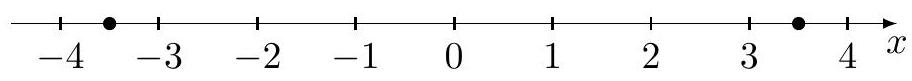
\includegraphics[max width=\textwidth, center]{2024_11_21_8f01584889ff06348ae7g-046(2)}\\
\(|x|<\frac{7}{2}\) czyli tych, których odległość od zera jest mniejsza od \(\frac{7}{2}\)\\
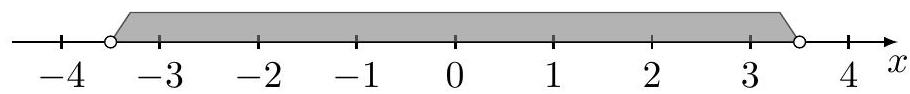
\includegraphics[max width=\textwidth, center]{2024_11_21_8f01584889ff06348ae7g-046(3)}\\
\(|x|>\frac{7}{2}\) czyli tych, których odległość od zera jest większa od \(\frac{7}{2}\)\\
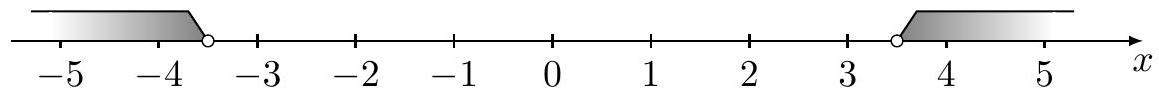
\includegraphics[max width=\textwidth, center]{2024_11_21_8f01584889ff06348ae7g-046(1)}\\
\(|x| \leqslant \frac{7}{2}\) czyli tych, których odległość od zera jest mniejsza lub równa \(\frac{7}{2}\)\\
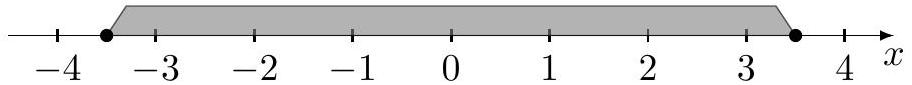
\includegraphics[max width=\textwidth, center]{2024_11_21_8f01584889ff06348ae7g-046}\\
\(|x| \geqslant \frac{7}{2}\) czyli tych, których odległość od zera jest większa lub równa \(\frac{7}{2}\)\\
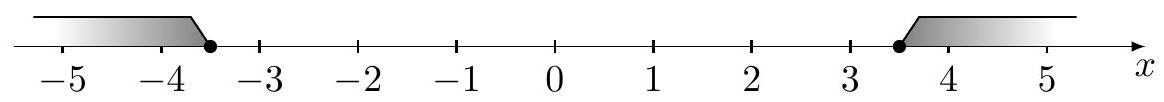
\includegraphics[max width=\textwidth, center]{2024_11_21_8f01584889ff06348ae7g-047}

\section*{UMOWA}
Kółko niezamalowane oznacza, że dana liczba nie należy, zaś kółko zamalowane oznacza, że dana liczba należy do zbioru liczb spełniających dany warunek.

\section*{UWAGA}
Symbol \(\geqslant\) oznacza nie mniejsze niż czyli większe lub równe, zaś\\
symbol \(\leqslant\) oznacza nie większe niż czylimniejsze lub równe.\\
62. Zaznacz na osi liczbowej te liczby, które spełniają warunek\\
a) \(|x|=2\)\\
b) \(|x| \geqslant 2\)\\
c) \(|x| \leqslant 1\)\\
63. Zaznacz na osi liczbowej te liczby, które spełniają warunek\\
a) odległość od zera jest równa 3\\
b) odległość od zera jest większa niż 3\\
c) odległość od zera jest nie większa niż 1\\
d) odległość od zera jest nie mniejsza niż \(\frac{1}{2}\)\\
e) odległość od zera jest większa niż 0\\
f) odległość od zera jest większa lub równa 0\\
g) odległość od zera jest mniejsza lub równa 0\\
64. Jakie wartości może przyjmować \(4 x\), jeżeli a) \(|4 x|=20 \quad\) b) \(|4 x|=8\).\\
65. Jakie wartości może przyjmować \(x\) jeżeli a) \(|4 x|=40, \quad\) b) \(|3 x|=15\).\\
66. Korzystając z powyższego wpierw zamień dane równanie na dwa równania bez wartości bezwzględnej, a następnie rozwiąż je\\
a) \(|3 x|=12\)\\
b) \(|5 x|=10\)\\
c) \(|5 x|=8\)\\
d) \(|7 x|=5\)\\
e) \(|3 x|=2\)\\
67. Jakie wartości może przyjmować \(x\) jeżeli\\
a) \(\frac{1}{2}|x|=2\),\\
b) \(2|x|=10\),\\
c) \(2|x|+3|x|=20\),\\
d) \(6|x|+4|x|=40\),\\
e) \(7|x|-5|x|=6\),\\
f) \(10|x|-2|x|-5|x|=3\).

\subsection*{2.5.2 Część całkowita liczby}
Obecnie wprowadzimy pojęcie część catkowita liczby. Mianowicie: częścią całkowitą liczby \(x\) jest największa liczba całkowita nie większa niż \(x\). Oznaczamy ją zazwyczaj \([x]\).

\section*{PRZYKŁADY}
\[
[3]=3 \quad[0]=0 \quad[-2]=-2 \quad[1,99]=1 \quad[-0,2]=-1 \quad[-1,9]=-2
\]

Poniżej na osi liczbowej zaznaczone są te wszystkie liczby, których część całkowita jest równa -2 oraz te wszystkie liczby, których część całkowita jest równa 1.\\
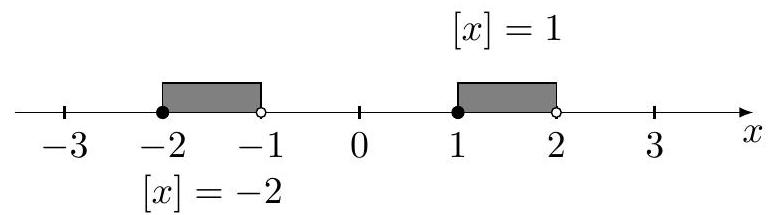
\includegraphics[max width=\textwidth, center]{2024_11_21_8f01584889ff06348ae7g-048}

Dla liczb większych lub równych -2 , a równocześnie mniejszych od -1 część całkowita równa jest -2 .

Dla liczb większych lub równych 1, a równocześnie mniejszych od 2 część całkowita równa jest 1.\\
68. Podaj trzy liczby, których część całkowita jest równa 0 oraz trzy liczby, których część całkowita jest równa -1 .\\
69. Zaznacz na osi liczbowej te wszystkie liczby, dla których\\
a) \([x]=0\),\\
b) \([x]=-1\),\\
c) \([x] \leqslant-1\),\\
d) \([x]>1\),\\
e) \([x]>-2\),\\
f) \([x]<-2\),\\
g) \([x] \leqslant-2\),\\
h) \([x]<-\frac{1}{2}\),\\
i) \([x]>0\),\\
j) \([x]>-\frac{5}{2}\),\\
k) \([x] \leqslant \frac{1}{3}\),\\
70. Podaj przykład trzech par liczb \((x, y)\), które spełniają poniższe warunki. Tam gdzie nie można podać trzech przykładów, podaj wszystkie przykłady\\
a) \(\left\{\begin{array}{l}x+y=4,9 \\ {[x]+[y]=3} \\ x>0, y>0\end{array}\right.\)\\
b) \(\left\{\begin{array}{l}x+y=3 \\ {[x]+[y]=3} \\ x>0, \quad y>0\end{array}\right.\)\\
c) \(\left\{\begin{array}{l}x+y=3 \\ {[x]+[y]=2} \\ x>0, \quad y>0\end{array}\right.\)\\
d) \(\left\{\begin{array}{l}x+y=-0,2 \\ {[x]+[y]=-2} \\ x \cdot y>0\end{array}\right.\)\\
e) \(\left\{\begin{array}{l}x+y=-0,5 \\ {[x]+[y]=-2} \\ x \cdot y<0\end{array}\right.\)\\
f) \(\left\{\begin{array}{l}x+y=3,8 \\ {[x]+[y]=2} \\ x \cdot y>0\end{array}\right.\)\\
g) \(\left\{\begin{array}{l}x+y=3,8 \\ {[x]+[y]=3}\end{array}\right.\)\\
h) \(\left\{\begin{array}{l}x+y=2 \\ {[x]+[y]=2} \\ x \cdot y>0\end{array}\right.\)\\
i) \(\left\{\begin{array}{l}x+y=2 \\ {[x]+[y]=1} \\ x \cdot y>0\end{array}\right.\)

\subsection*{2.5.3 Część ułamkowa liczby}
Część ułamkowa liczby powstaje przez odjęcie od danej liczby jej części całkowitej. Część ułamkową liczby \(x\) oznaczamy \(\{x\}\), a zatem \(\{x\}=x-[x]\)

\section*{PRZYKŁADY}
liczba \(x \quad\) część całkowita liczby \([x] \quad\) część ułamkowa liczby \(\{x\}\)

\begin{center}
\begin{tabular}{lll}
\(7 \frac{1}{2}\) & 7 & \(7 \frac{1}{2}-7=\frac{1}{2}\) \\
0,95 & 0 & \(0,95-0=0,95\) \\
3 & 3 & \(3-3=0\) \\
\(-0,7\) & -1 & \(-0,7-(-1)=0,3\) \\
\end{tabular}
\end{center}

\begin{enumerate}
  \setcounter{enumi}{70}
  \item Podaj takie trzy pary liczb \(x\) i \(y\) aby \(x+y=2 \mathrm{i}\{x+y\}=0\).
  \item Podaj takie trzy pary różnych liczb \(x\) i \(y\), że \(\{x\}+\{y\}=1\), zaś \(\{x+y\}=0\).
  \item Podaj takie trzy trójki różnych liczb \(x, y, z\) że \(\{x\}+\{y\}+\{z\}=2\), zaś \(x+y+z=6\)
  \item Podaj takie trzy trójki różnych liczb \(x, y, z\) że \(x+y+z=7\), zaś \(\{x\}+\{y\}+\{z\}=2\).
  \item Podaj takie trzy trójki różnych liczb \(x, y, z\) że\\
a) \(\{x+y+z\}=0 \quad\) i \(\quad\{x\}+\{y\}+\{z\}=1\)\\
b) \([x]+[y]+\{z\}=\frac{1}{2} \quad\) i \(\quad\{x+y+z\}=0\)\\
c) \([x+y+z]=0 \quad\) i \(\quad\{x+y+z\}=\frac{1}{2}\)
\end{enumerate}

\subsection*{2.5.4 Algorytm Euklidesa}
Algorytm Euklidesa jest to sposób wyznaczania największego wspólnego dzielnika dwóch liczb, bez konieczności rozkładania tych liczb na czynniki pierwsze. Algorytm ten korzysta z faktu, że \(\operatorname{NWD}(a, a)=a, \operatorname{NWD}(a, b)=\) \(\operatorname{NWD}(b, a)\) oraz z faktu, który można uzasadnić (spróbuj), że jeżeli od większej liczby z dwóch danych liczb naturalnych odejmiemy mniejszą liczbę, to\\
ta mniejsza liczba oraz otrzymana różnica mają taki sam wspólny dzielnik jak para liczb wyjściowych. Bardziej formalnie zapisujemy to następująco:

\[
\text { Jeżeli } a>b, \quad \text { to } \quad \operatorname{NWD}(a, b)=\operatorname{NWD}(a-b, b) \text {. }
\]

Ten proces zmniejszania liczb kończymy wówczas, gdy obie liczby są równe.

\section*{PRZYKŁADY}
a) \(\operatorname{NWD}(18,24)=\operatorname{NWD}(18,6)=\operatorname{NWD}(12,6)=\operatorname{NWD}(6,6)=6\)\\
b) \(\operatorname{NWD}(17,5)=\operatorname{NWD}(12,5)=\operatorname{NWD}(7,5)=\operatorname{NWD}(2,5)=\operatorname{NWD}(2,3)=\) \(\operatorname{NWD}(2,1)=\operatorname{NWD}(1,1)=1\)\\
c) \(\operatorname{NWD}(114,354)=\operatorname{NWD}(240,114)=\operatorname{NWD}(126,114)=\operatorname{NWD}(12,114)=\) \(\operatorname{NWD}(12,102)=\operatorname{NWD}(12,90)=\ldots=\operatorname{NWD}(12,6)=\operatorname{NWD}(6,6)=6\)\\
zauważ, że\\
\(\operatorname{NWD}(114,354)=\operatorname{NWD}(114,12)\)\\
czyli\\
\(\operatorname{NWD}(114,354)=\operatorname{NWD}(114, \underbrace{354-3 \cdot 114}_{=12})\)

\section*{WNIOSEK}
\[
\operatorname{NWD}(a, b)=\operatorname{NWD}(a-k \cdot b, b)
\]

\begin{enumerate}
  \setcounter{enumi}{75}
  \item Wyznacz w podobny sposób\\
(a) \(\operatorname{NWD}(66,12)\)\\
(b) \(\operatorname{NWD}(91,28)\)\\
(c) \(\operatorname{NWD}(420,516)\)\\
(d) \(\operatorname{NWD}(143,1309)\)\\
(e) \(\operatorname{NWD}(1001,3705)\)
\end{enumerate}

\section*{Odpowiedzi}
\begin{enumerate}
  \item a) 79 b) 484 c) 169 d) 200 e) 375 f) 878 g) 149 h) 228 i) 849
  \item a) 230 b) 30 c) 130 d) 280 e) 270 f) 170 g) 340 h) 260 i) 180
  \item a) \(6,8,10,12,14,16\) b) \(15,20,25,30,35\) c) \(21,28,35,42,49\)
  \item a) 1,7 b) \(1,5,7,35\) c) \(1,2,4,8,16\) d) \(1,5,25,125\)\\
e) \(1,2,3,4,6,8,12,24\) f) \(1,2,3,4,5,6,10,12,15,20,30,60\)
  \item liczbami pierwszymi z tego zakresu są 11, 13, 17, 19, 23, 29, 31, 37
  \item а) \(24=2 \cdot 2 \cdot 2 \cdot 3,45=3 \cdot 3 \cdot 5\), \(\operatorname{NWD}(24,45)=3\)\\
b) \(24=2 \cdot 2 \cdot 2 \cdot 3,65=5 \cdot 13, \operatorname{NWD}(24,65)=1\)\\
c) \(18=2 \cdot 3 \cdot 3,30=2 \cdot 3 \cdot 5, \operatorname{NWD}(18,30)=6\)\\
d) \(114=2 \cdot 57=2 \cdot 3 \cdot 19,36=2 \cdot 2 \cdot 3 \cdot 3, \operatorname{NWD}(114,36)=6\)\\
e) \(10=2 \cdot 5,15=3 \cdot 5, \operatorname{NWD}(10,15)=5\)\\
f) \(60=2 \cdot 2 \cdot 3 \cdot 5,50=2 \cdot 5 \cdot 5, \operatorname{NWD}(60,50)=10\)\\
g) \(195=5 \cdot 39=3 \cdot 5 \cdot 13,30=2 \cdot 3 \cdot 5, \operatorname{NWD}(195,30)=15\)
  \item a) 12 b) 60 c) 105 d) 84 e) 60 f) 90 g) 72 h) 225 i) 420
  \item a) 22 b) 18 c) 16 d) 28 e) 0 f) 12 g) 18 h) 6 i) -2 j) 6 k) 40 l) 50
  \item a) 1300 b) 160000 c) 300 d) 180 e) 480 f) 420 g) 1400 h) 2400\\
i) 270 j) 1300 k\() 1900 \mathrm{l}) 800 \mathrm{~m}) 11 \cdot \triangle \mathrm{n}) 23 \cdot\)
  \item a) 8 b) 2 c) 16 d) 144
  \item a) 14 b) -11 c) 6 d) 0 e) 30 f) 4 g) -27 h) -2 i) -20 j) 49 k) 2 l) \(-40 \mathrm{~m}) 2 \mathrm{n})-7\)
  \item a) 75 b) 300 c) 720 d) 252 e) 21 f) 90 g) 3 h) 33 i) -4 j) 13 k) -15 l) \(-61 \mathrm{~m}) 20 \mathrm{n})-123\) o) -21
  \item a) -4 b) 43 c) 44 d) -53 e) 43 f) -43 g) -43 h) -43 i) -103 j) -12 k) 53 l) 84 m\()-43 \mathrm{n})-12\) o) -80
  \item a) \(2 \frac{4}{7}\) b) \(-5 \frac{1}{3}\) c) \(-3 \frac{4}{11}\) d) \(13 \frac{1}{11}\) e) \(10 \frac{2}{3}\) f) -17 g) \(-23 \frac{1}{13}\) h) 20\\
i) -19 j) \(-36 \mathrm{k})-18\) l) 63
  \item a) 2 b) \(\frac{2}{15}\) c) \(\frac{5}{9}\) d) \(\frac{1}{5}\) e) \(\frac{3}{4}\) f) \(2 \frac{1}{2}\) g) \(\frac{1}{2}\) h) \(\frac{1}{6}\) i) \(\frac{3}{4}\) j) \(\frac{8}{55}\) k) 6\\
l) \(\left.\left.\frac{5}{6} \mathrm{~m}\right) 14 \mathrm{n}\right) 34 \frac{2}{7}\) o) \(\left.\frac{5}{8} \mathrm{p}\right) 5\) q) \(\frac{1}{2}\) r) \(1 \frac{2}{5}\) s) 5 t) \(\left.\left.13 \frac{1}{3} \mathrm{u}\right) 3 \mathrm{v}\right) \frac{5}{6}\) w) \(\frac{5}{7}\)
  \item a) \(8 \frac{1}{5}\) b) \(\frac{71}{72}\) c) \(20 \frac{30}{77}\) d) \(10 \frac{4}{21}\) e) \(6 \frac{10}{33}\) f) \(8 \frac{16}{105}\) g) \(25 \frac{8}{9}\) h) \(\frac{13}{482}\)\\
i) \(4023 \frac{19}{4024}\)
  \item a) \(7 \frac{2}{7}\) b) \(50 \frac{2}{3}\) c) \(2 \frac{5}{7}\) d) \(20 \frac{28}{41}\) e) \(26 \frac{7}{8}\) f) \(5 \frac{6}{7}\) g) \(2 \frac{5}{6}\) h) \(2 \frac{5}{28}\) i) \(2 \frac{59}{66}\)
  \item a) \(1 \frac{3}{4}\) b) \(2 \frac{1}{45}\) c) \(2 \frac{8}{15}\) d) \(5 \frac{14}{15}\) e) \(28 \frac{11}{40}\) f) \(3 \frac{27}{40}\) g) \(1 \frac{111}{200}\) h) \(2 \frac{5}{72}\)\\
i) \(3 \frac{127}{150}\)
  \item a) \(2 \frac{2}{5}\) b) \(13 \frac{13}{15}\) c) \(8 \frac{1}{2}\) d) \(2 \frac{4}{9}\)
  \item a) \(1 \frac{2}{3}\) b) \(2 \frac{1}{3}\) c) \(37 \frac{1}{2}\) d) 69 e) 76 f) 129 g) \(4 \frac{4}{5}\) h) 4 i) 14
  \item a) \(\frac{3}{4}\) b) \(\frac{5}{12}\) c) \(\frac{22}{49}\) d) 10 e) \(66 \frac{1}{2}\) f) \(20 \frac{4}{7}\)
  \item a) \(1 \frac{3}{4}\) b) \(2 \frac{1}{5}\) c) 3 d) \(3 \frac{3}{4}\) e) \(2 \frac{3}{5}\) f) \(\frac{3}{7}\) g) \(\frac{7}{36}\) h) \(\frac{6}{37}\)
  \item a) 1 b) 12 c) 49 d) \(8 \frac{3}{4}\) e) \(10 \frac{2}{7}\) f) 2 g) \(\frac{3}{8}\) h) \(\frac{2}{5}\) i) \(18 \frac{2}{3}\) j) 132\\
k) 70 l) \(1 \frac{3}{7} \mathrm{~m}\) ) 12 n\() 33\) o) \(\left.13 \frac{1}{5} \mathrm{p}\right) \frac{3}{10}\)
  \item 140 uczniów
  \item 120 uczniów
  \item \(53 \frac{3}{11} \mathrm{~kg}\)\\
45.12
  \item a) \(\frac{83}{110}\) b) 16 c) \(\frac{25}{4}\) d) \(\frac{13}{15}\) e) \(\frac{1}{2}\) f) \(\frac{1}{3}\) g) \(\frac{4}{5}\) h) \(4 \frac{1}{4}\) i) 25 j) \(\frac{62}{15}\)\\
k) \(\frac{1}{3}\) l) \(\frac{1}{6} \mathrm{~m}\) ) \(\frac{5}{3}\) n) \(\frac{11}{7}\) o) \(\frac{82}{29}\) p) 72
  \item a) \(10^{9}\) b) \(10^{7}\) c) \(10^{11}\) d) \(10^{16}\) e) \(10^{18}\) f) \(10^{12}\) g) \(10^{8}\) h) \(10^{14}\)
  \item a) \(10^{3}\) b) 1 c) \(10^{15}\) d) \(10^{5}\) e) \(\frac{1}{10^{6}}\) f) \(10^{12}\) g) \(\frac{1}{10^{7}}\) h) \(10^{11}\) i) \(10^{17}\)
  \item a) \(10^{60}\) b) \(10^{80}\) c) \(10^{90}\) d) \(10^{300}\) e) \(10^{990}\) f) \(10^{200}\)
  \item a) \(5 \cdot 10^{4}\) b) \(2,5 \cdot 10^{3}\) c) \(2,5 \cdot 10\) d) \(1,23 \cdot 10^{5}\) e) \(1,23456 \cdot 10\)\\
f) \(1,23456 \cdot 10^{2}\) g) \(2 \cdot 10^{4}\) h) \(2,30032 \cdot 10^{5}\) i) \(2,0100102 \cdot 10^{3}\)
  \item a) 20000 b) 5000000 c) 25000000 d) 34500 e) 3112000\\
f) 302000 g\() 32000 \mathrm{~h}) 7500\) i) 7500
  \item a) \(5,10 \cdot 10^{8}\) b) \(1,08 \cdot 10^{12}\) c) \(3,00 \cdot 10^{8}\) d) \(8,64 \cdot 10^{4}\) e) \(3,15 \cdot 10^{7}\)
  \item a) \(3,3 \cdot 10^{12}\) b) \(4 \cdot 10^{7}\) c) \(6 \cdot 10^{8}\) d) \(2,8 \cdot 10^{10}\) e) \(1,1 \cdot 10^{16}\) f) \(5,6 \cdot 10^{18}\) g) \(1,08 \cdot 10^{18}\) h) \(1,575 \cdot 10^{12}\) i) \(2,87 \cdot 10^{16}\) j) \(\left.3,6 \cdot 10^{8} \mathrm{k}\right) 6,25 \cdot 10^{6}\) l) \(2 \cdot 10^{6}\) 58. a) \(3 \cdot 10^{6}\) b) \(1,04 \cdot 10^{10}\) c) \(1,25 \cdot 10\) d) \(1,5 \cdot 10^{4}\) e) \(7,5 \cdot 10^{4}\) f) \(7,5 \cdot 10^{8}\) g) \(\left.2,5 \cdot 10^{3} \mathrm{~h}\right) 4 \cdot 10^{2}\) i) \(6 \cdot 10^{7}\)
  \item a) \(8 \cdot 10^{15}\)\\
b) \(2 \cdot 10^{15}\)\\
c) \(1,25 \cdot 10^{20}\)\\
d) \(5 \cdot 10^{18}\)\\
e) \(6,25 \cdot 10^{6}\)\\
f) \(2,5 \cdot 10^{6}\)\\
g) \(\left.6,4 \cdot 10^{13} \mathrm{~h}\right) 4 \cdot 10^{13}\)
  \item a) \(8 \cdot 10^{12}\) b) \(9 \cdot 10^{3}\) c) \(9,7 \cdot 10^{8}\) d) \(7,8 \cdot 10^{2}\) e) \(1,5 \cdot 10^{16}\) f) \(1,3 \cdot 10^{3}\)\\
g) \(\left.2,2 \cdot 10^{4} \mathrm{~h}\right) 1,61 \cdot 10^{13}\) i) \(6 \cdot 10^{4}\) j) \(2,5 \cdot 10^{4} \mathrm{k}\) ) \(1,7 \cdot 10^{2}\) l) \(1,35 \cdot 10^{3}\)\\
m) \(\left.1,973 \cdot 10^{6} \mathrm{n}\right) 1,1 \cdot 10^{3}\) o) \(9 \cdot 10^{3}\) p) \(7,1 \cdot 10^{13}\) q) \(1,3 \cdot 10^{16}\) r) \(1,11 \cdot 10^{10}\)\\
s) \(1,03 \cdot 10^{12}\) t) \(8,52 \cdot 10^{16}\) u) \(2,3063 \cdot 10^{7}\) v) \(2,5 \cdot 10^{9}\) w) \(7,8 \cdot 10^{4}\)
  \item a) \(1,1 \cdot 10^{5}\) b) \(3 \cdot 10^{3}\) c) \(8,8 \cdot 10^{9}\) d) \(1,3 \cdot 10^{3}\) e) \(9 \cdot 10^{2}\) f) \(4 \cdot 10^{4}\)\\
g) \(3,7 \cdot 10^{3}\) h) \(3,7 \cdot 10^{2}\) i) \(3 \cdot 10^{13}\) j) \(7 \cdot 10^{9}\)
\end{enumerate}

\section*{Rozdział 3}
\section*{JEDNOSTKI W FIZYCE}
W tym rozdziale będziemy zajmować się niektórymi jednostkami używanymi przede wszystkim w fizyce. Umiejętność operowania jednostkami jest ważna, a przy tym przydatna w życiu codziennym. Celem nauki matematyki na pewnym poziomie jest \href{http://m.in}{m.in}. nabycie dobrej kontroli nad językiem, a elementem tego jest poprawne posługiwanie się jednostkami. Innym celem jaki realizujemy w trakcie robienia tych ćwiczeń jest wykształcenie sprawnego umysłu, a nie ustalenie za wszelką cenę poprawnej odpowiedzi, dlatego w ćwiczeniach tych nie należy używać kalkulatora. Nie ma żadnej lekkiej drogi w kształtowaniu sprawnego umysłu.

\subsection*{2.1 Czas}
Będziemy posługiwać się następującymi czterema jednostkami czasu:

\begin{verbatim}
1 doba = a g godziny
1 godzina (1 h) = 60 minut
1 minuta (1 min) = 60 sekund
1 sekunda (1 s)
\end{verbatim}

\begin{enumerate}
  \item Ile sekund jest w jednej godzinie? Ile minut jest w jednej dobie? Ile sekund jest w jednej dobie?
  \item Wyraź następującą część godziny\\
a) \(\frac{1}{2}\)\\
b) \(\frac{1}{3}\)\\
c) \(\frac{1}{4}\)\\
d) \(\frac{1}{5}\)\\
e) \(\frac{1}{6}\)\\
f) \(\frac{1}{10}\)\\
g) \(\frac{1}{12}\)\\
h) \(\frac{1}{15}\)\\
i) \(\frac{1}{20}\)\\
j) \(\frac{1}{30}\)\\
w minutach.
  \item Wyraź następującą część godziny\\
a) \(\frac{2}{3}\)\\
b) \(\frac{3}{4}\)\\
c) \(\frac{2}{5}\)\\
d) \(\frac{11}{15}\)\\
e) \(\frac{5}{6}\)\\
f) \(\frac{3}{10}\)\\
g) \(\frac{5}{12}\)\\
h) \(\frac{11}{12}\)\\
i) \(\frac{4}{15}\)\\
j) \(\frac{17}{20}\)\\
w sekundach.
  \item Wyraź następującą liczbę godzin\\
a) \(2 \frac{7}{30}\)\\
b) \(3 \frac{5}{12}\)\\
c) \(2 \frac{3}{20}\)\\
d) \(1 \frac{43}{60}\)\\
e) \(2 \frac{21}{30}\) w minutach.
  \item Jaka to część godziny?\\
a) 15 min\\
b) 25 min\\
c) 27 min\\
d) 9 min\\
e) 35 min\\
f) 40 min\\
g) 55 min\\
h) 45 min\\
i) 57 min\\
j) 24 min\\
k) 14 min\\
l) 22 min\\
m) 108 min\\
n) 96 min\\
o) 99 min\\
p) 125 min\\
q) 93 min\\
r) 95 min\\
s) 186 min\\
t) 129 min
\end{enumerate}

Wynik podaj w postaci ułamka nieskracalnego względnie też liczby mieszanej.

\subsection*{2.2 Odległość, długość}
Chociaż w praktyce będziemy posługiwali się tylko jednostkami metrycznymi, to dla nabycia pewnej swobody w przeliczaniu różnych jednostek, podajemy dodatkowo kilka jednostek, będących w krajach anglosaskich w mniej lub bardziej powszechnym użyciu.

\begin{itemize}
  \item metryczne\\
a) \(1 \operatorname{metr}(1 \mathrm{~m}) \quad=100\) centymetrów\\
b) 1 kilometr \((1 \mathrm{~km})=1000\) metrów\\
c) 1 decymetr \((1 \mathrm{dm})=1 / 10\) metra \(=10\) centymetrów\\
d) 1 centymetr \((1 \mathrm{~cm})=1 / 100\) metra\\
e) 1 milimetr \((1 \mathrm{~mm})=1 / 1000\) metra\\
f) 1 centymetr \(=10\) milimetrów
  \item niemetryczne\\
a) 1 mila angielska ( 1 mile \()=1760\) yardów \(=1609,344 \mathrm{~m}\)\\
b) 1 jard ( 1 yd )\\
\(=0,914 \mathrm{~m}\)\\
c) 1 stopa \((1 \mathrm{ft}) \quad=1 / 3\) jarda \(=30,5\) centymetra\\
d) \(1 \mathrm{cal}(1 \mathrm{in}) \quad=1 / 12\) stopy \(=2,54\) centymetra\\
mila morska (nautical mile) - jednostka długości \(=1852 \mathrm{~m}\), stosowana w żegludze morskiej, dzieli się na 10 kabli, czyli 1 kabel \(=185,2 \mathrm{~m}\).
\end{itemize}

\begin{enumerate}
  \setcounter{enumi}{5}
  \item Wyraź w centymetrach następujące długości\\
a) 3 m\\
b) 900 mm\\
c) \(30,7 \mathrm{~m}\)\\
d) \(6,5 \mathrm{~m}\)\\
e) 450 mm\\
f) 35 mm\\
g) 7 mm\\
h) 5 yd\\
i) 4 ft\\
j) 5 in
  \item Wyraź w metrach następujące odległości:\\
a) \(1,703 \mathrm{~km}\)\\
b) \(2,42 \mathrm{~km}\)\\
c) \(0,331 \mathrm{~km}\)\\
d) \(0,9 \mathrm{~km}\)\\
e) 305 cm\\
f) 782 cm\\
g) 78 cm\\
h) 1122 cm\\
i) 2000 mm\\
j) 4200 mm\\
k) 3430 mm\\
l) 1025 mm\\
m) 18 km\\
n) \(36,5 \mathrm{~km}\)\\
o) \(92,34 \mathrm{~km}\)\\
p) \(3,456 \mathrm{~km}\)\\
q) 11 yd\\
r) 15 ft\\
s) 17 in\\
t) 6 ft 2 in\\
u) \(\frac{1}{9}\) mile\\
v) 100 yd\\
w) 150 yd 6 ft
\end{enumerate}

\subsection*{2.3 Prędkość}
Chociaż w fizyce rozróżnia się pojęcia prędkość i szybkość, różnica pomiędzy którymi zostanie z czasem wyjaśniona, to my na razie, będziemy traktować te terminy jako równoważne. W zadaniach poniższych będzie występować tylko tzw. prędkość średnia, która określona jest następująco:

\[
\text { prędkość średnia }=\frac{\text { droga jaką przebyło ciało }}{\text { czas w jakim przebyło tę drogę }}\left[\frac{\text { jedn. długości }}{\text { jedn. czasu }}\right]
\]

czyli krótko (pamiętając oczywiście o jednostkach!!!)

\[
v=\frac{s}{t}
\]

gdzie \(v\) oznacza prędkość, \(s\) - drogę, a \(t\) - czas w jakim ta droga została przebyta. Ponieważ tutaj jest mowa tylko o prędkości średniej, dlatego będziemy mówili krótko prędkość.

\section*{PRZYKŁAD 1}
Pojazd przebył drogę 80 km w ciągu 1 godziny, mówimy wówczas, że jego średnia prędkość wynosiła \(\frac{80}{1} \frac{[\mathrm{~km}]}{[\operatorname{godz}]}\), co zapisujemy krócej \(80 \mathrm{~km} / \mathrm{h}\).

\section*{UWAGA}
Zapis \(1 \mathrm{~km} / \mathrm{h}\) czy też \(1 \frac{\mathrm{~km}}{\mathrm{~h}}\) oznacza \(\frac{1 \mathrm{~km}}{1 \mathrm{~h}}\).

\section*{PRZYKŁAD 2}
Pojazd przebył 200 kilometrów w ciągu 4 godzin, oznacza to, że jego średnia prędkość

\[
v_{\mathrm{s} \mathrm{r}}=\frac{200 \mathrm{~km}}{4 \mathrm{~h}}=50 \mathrm{~km} / \mathrm{h} .
\]

PRZYKŁAD 3\\
Jacek przeszedł 12 kilometrów w ciągu 2 godzin. Jaka była jego średnia prędkość wyrażona w km/h, a jaka w m/min?

\[
\frac{12 \mathrm{~km}}{2 \mathrm{~h}}=\frac{6 \mathrm{~km}}{1 \mathrm{~h}}=\frac{6000 \mathrm{~m}}{60 \mathrm{~min}}=100 \mathrm{~m} / \mathrm{min}
\]

\section*{PRZYKŁAD 4}
Pojazd przejechał 120 kilometrów w ciągu \(2 \frac{1}{2}\) godziny. Jaka była jego średnia prędkość w km/h, jaka w m/min, a jaka w cm/s?

\[
\frac{120 \mathrm{~km}}{2 \frac{1}{2} \mathrm{~h}} \mathrm{~km} / \mathrm{h}=\frac{240}{5} \mathrm{~km} / \mathrm{h}=48 \mathrm{~km} / \mathrm{h}
\]

\(48 \mathrm{~km} / \mathrm{h}=\frac{48000 \mathrm{~m}}{60 \mathrm{~min}}=800 \mathrm{~m} / \mathrm{min}\).\\
\(800 \mathrm{~m} / \mathrm{min}=\frac{80000 \mathrm{~cm}}{60 \mathrm{~s}}=1333 \frac{1}{3} \mathrm{~cm} / \mathrm{s}\).\\
8. Wyraź prędkość \(1 \mathrm{~km} / \mathrm{h} \mathrm{w}\)\\
a) \(\mathrm{m} / \mathrm{min}\)\\
b) \(\mathrm{m} / \mathrm{s}\)\\
c) \(\mathrm{cm} / \mathrm{s}\)\\
9. Jacek szedł przez \(2 \frac{1}{5}\) godziny z prędkością \(6 \mathrm{~km} / \mathrm{h}\).\\
a) Ile metrów przeszedł Jacek w tym czasie?\\
b) Wyraź czas jego marszu w minutach, a następnie w sekundach.\\
c) Wyraź jego prędkość w

\begin{enumerate}
  \item \(\mathrm{m} / \mathrm{min}\)
  \item \(\mathrm{m} / \mathrm{s}\)
  \item \(\mathrm{cm} / \mathrm{s}\)
\end{enumerate}

Związek między przebytą drogą \(s\), czasem \(t\) w jakim ona została przebyta, i prędkością \(v\) z jaką ta droga została przebyta jest następujący

\[
s=v \cdot t
\]

Oczywiście muszą być te wielkości wyrażone w odpowiednich jednostkach. Związek ten można również wyrazić w postaci

\[
t=\frac{s}{v}, \quad \text { czy też } \quad v=\frac{s}{t} .
\]

\begin{enumerate}
  \setcounter{enumi}{9}
  \item Pływak przepłynął 200 m w czasie 1 min 48 s .\\
a) Oblicz jego prędkość w m/s\\
b) Oblicz ile centymetrów przepływał on w czasie \(1 / 10\) sekundy, a ile w czasie \(1 / 100\) sekundy.
\end{enumerate}

Prędkość dźwięku w powietrzu wynosi \(340 \mathrm{~m} / \mathrm{s}\). W lotnictwie wojskowym używa się czasami jednostki prędkości zwanej machem, przy czym 1 mach jest to prędkość dźwięku w powietrzu i oznacza liczbę kilometrów jaką dźwięk pokona w ciągu godziny.\\
11. Wyraź prędkość 1 macha w a) \(\mathrm{km} / \mathrm{h} \quad\) b) \(\mathrm{m} / \mathrm{min} \quad c) \mathrm{km} / \mathrm{s} \quad\) d) \(\mathrm{km} / \mathrm{min}\)\\
12. Samolot leciał z prędkością 2,2 macha. Wyraź prędkość tego samolotu w\\
a) \(\mathrm{km} / \mathrm{h}\)\\
b) \(\mathrm{km} / \mathrm{min}\)\\
c) \(\mathrm{km} / \mathrm{s}\)

Prędkość statków wyraża się najczęściej w węzłach. Jeden węzel jest to prędkość 1 mila morska/godzinę.\\
13. Wyraź prędkość 1 węzła w\\
a) \(\mathrm{m} / \mathrm{min}\)\\
b) \(\mathrm{km} / \mathrm{h}\)\\
14. Statek płynie z prędkością 18 węzłów. Wyraź jego prędkość w\\
a) \(\mathrm{km} / \mathrm{h}\)\\
b) \(\mathrm{m} / \mathrm{s}\).\\
15. Statek płynie z prędkością \(37 \mathrm{~km} / \mathrm{h}\). Wyraź jego prędkość w węzłach.\\
16. Samochód jechał przez\\
a) 3 h\\
z prędkością\\
\(24 \mathrm{~km} / \mathrm{h}\)\\
b) \(2 \frac{1}{2} \mathrm{~h}\)\\
z prędkością\\
30 km/h\\
c) \(1 \frac{1}{4} \mathrm{~h}\)\\
z prędkością\\
40 km/h\\
d) 20 min\\
z prędkością\\
\(72 \mathrm{~km} / \mathrm{h}\)\\
e) 5 min\\
z prędkością\\
90 km/h\\
f) 1 h 30 min\\
z prędkością \(\quad 40 \mathrm{~km} / \mathrm{h}\)\\
g) 2 h 35 min\\
z prędkością \(48 \mathrm{~km} / \mathrm{h}\)\\
h) 1 h 24 min\\
z prędkością\\
60 km/h

Ile kilometrów przejechał ten pojazd w każdym z powyższych przypadków?\\
17. Marcin przyjeżdża do dziadka na wieś. Dziadek mieszka w odległości \(3,6 \mathrm{~km}\) od stacji. O której godzinie dziadek musi wyjść z domu, aby zdążyć na przybywający o godzinie 10:00 pociąg, którym przyjeżdża wnuczek, jeżeli chodzi on z szybkością \(3 \mathrm{~km} / \mathrm{h}\) ?\\
18. Pociąg wyjechał z miejscowości \(A\) o godzinie 16:00 i musi dojechać do miejscowości \(C\) o godzinie 21:30. Przez pierwsze trzy godziny jechał z szybkością \(60 \mathrm{~km} / \mathrm{h}\). W miejscowości \(B\) zatrzymał się na pół godziny. Z jaką szybkością musi przejechać pozostałą część trasy, jeżeli z \(B\) do \(C\) pozostały jeszcze 124 kilometry?\\
19. Jacek przez półtorej godziny przeszedł 6 kilometrów. Ile kilometrów przejdzie on w ciągu 4 godzin, jeżeli przez cały czas szedł z tą samą prędkością?\\
20. Robert umówił się z kolegami nad jeziorem o godzinie 10:20. Z domu wyruszył on o godzinie 9:00. Z jaką prędkością musi on iść aby zdążyć na czas, jeżeli odległość z domu do jeziora wynosi 10 km ?\\
21. Dwa zespoły robocze przebijają z dwóch stron tunel długości 253 metrów. Pierwszy zespół przebija 5 metrów dziennie, a drugi 6 metrów dziennie. Po ilu dniach zespoły się spotkają?\\
22. Odległość z Warszawy do Poznania wynosi 300 km. Jeden samochód wyrusza z Warszawy i jedzie do Poznania z prędkością \(80 \mathrm{~km} / \mathrm{h}\). W tej samej chwili wyrusza z Poznania do Warszawy drugi samochód, który jedzie z prędkością \(120 \mathrm{~km} / \mathrm{h}\). Po jakim czasie te dwa samochody się miną?\\
23. Dwaj rowerzyści wyruszają naprzeciwko siebie z miast \(A\) i \(B\) odległych o 105 km . Pierwszy z nich jedzie z prędkością \(15 \mathrm{~km} / \mathrm{h}\), a drugi \(20 \mathrm{~km} / \mathrm{h}\). Po jakim czasie oni się spotkają?\\
24. Motocykl i autobus ruszają równocześnie w tym samym kierunku. Prędkość autobusu wynosi \(40 \mathrm{~km} / \mathrm{h}\), zaś prędkość motocykla wynosi \(75 \mathrm{~km} / \mathrm{h}\). Jaka będzie odległość między nimi po upływie 4 godzin?\\
25. Naprzeciwko siebie jadą dwaj rowerzyści. Jeden jedzie z prędkością \(12 \mathrm{~km} / \mathrm{h}\), a drugi o trzy kilometry na godzinę więcej. W pewnym momencie mijają się. W jakiej będą oni odległości od siebie w dwie godziny po minięciu się?\\
26. Janek i Marek biegną z przeciwnych kierunków, a są oddaleni od siebie o 200 metrów. Janek biegnie z szybkością \(6 \mathrm{~m} / \mathrm{sek}\), a Marek \(4 \mathrm{~m} / \mathrm{sek}\). Po jakim czasie oni spotkają się? Po jakim czasie od momentu rozpoczęcia biegu odległość pomiędzy nimi będzie wynosiła ponownie 200 metrów?\\
27. Odległość z miejscowości A do miejscowości B wynosi 600 kilometrów. Ze stacji A wyrusza pociąg w kierunku B z prędkością \(50 \mathrm{~km} / \mathrm{h}\), a w tej samej chwili wyrusza z B w kierunku A pociąg z prędkością \(70 \mathrm{~km} / \mathrm{h}\). Jaka będzie odległość pomiędzy pociągami po upływie 2 godzin? Po ilu godzinach od chwili wyruszenia ze stacji spotkają się te pociągi?\\
28. Z dwóch miejscowości odległych o 390 km wyruszyły jednocześnie naprzeciw siebie dwa samochody. Pierwszy jechał ze średnią prędkością \(70 \mathrm{~km} / \mathrm{h}\), a drugi \(60 \mathrm{~km} / \mathrm{h}\). Po ilu godzinach jazdy samochody się spotkają? Ile kilometrów przejechał każdy samochód do chwili spotkania?\\
29. Z dwóch przystani odległych od siebie o 130 km , jednocześnie wypłynęły naprzeciw siebie łódka i statek. Łódka płynęła z prędkością 4 km na godzinę, a statek z prędkością 16 km na godzinę. Ile kilometrów przepłynie łódka do momentu gdy odległość między nimi będzie wynosiła 10 km ?\\
30. Z miejscowości A w przeciwnych kierunkach wyjechali o tej samej porze dwaj kolarze. Pierwszy jechał z prędkością \(20 \mathrm{~km} /\) godz, a drugi z prędkością \(25 \mathrm{~km} /\) godz. Jaka będzie odległość między kolarzami po 3 godzinach jazdy? A jaka byłaby odpowiedź, gdyby wyruszyli oni równocześnie w tym samym kierunku?\\
31. Rowerzysta i motocyklista wyruszają równocześnie z tego samego punktu jadąc w tym samym kierunku. Rowerzysta jedzie z prędkością \(20 \mathrm{~km} / \mathrm{h}\), a motocyklista \(80 \mathrm{~km} / \mathrm{h}\). Jaka będzie odległość pomiędzy nimi po upływie pół godziny? Po jakim czasie odległość pomiędzy nimi wyniesie 90 km ?

\subsection*{2.4 Powierzchnia}
Będziemy używali następujących jednostek powierzchni:\\
\(1 \mathrm{~mm}^{2}\) jest to powierzchnia kwadratu o boku długości 1 mm\\
\(1 \mathrm{~cm}^{2}\) jest to powierzchnia kwadratu o boku długości 1 cm\\
\(1 \mathrm{~m}^{2}\) jest to powierzchnia kwadratu o boku długości 1 m\\
\(1 \mathrm{~km}^{2}\) jest to powierzchnia kwadratu o boku długości 1 km\\
1 ar jest to powierzchnia kwadratu o boku długości 10 m\\
1 hektar jest to powierzchnia kwadratu o boku długości 100 m\\
32. Uzupełnij:\\
a) \(1 \mathrm{~km}^{2}=\ldots \ldots\) ha\\
b) \(1 \mathrm{~km}^{2}=\ldots \ldots \ldots\) ar\\
c) \(1 \mathrm{~km}^{2}=\ldots \ldots \mathrm{m}^{2}\)\\
d) \(1 \mathrm{ha} \quad=\ldots \ldots \mathrm{m}^{2}\)\\
e) \(1 \mathrm{ar}=\ldots \ldots \ldots \mathrm{m}^{2}\)\\
f) \(1 \mathrm{~m}^{2}=\ldots \ldots \ldots \mathrm{cm}^{2}\)\\
g) \(1 \mathrm{~cm}^{2}=\ldots \ldots \mathrm{mm}^{2}\)\\
h) \(1 \mathrm{~m}^{2}=\ldots \ldots \ldots \mathrm{mm}^{2}\)\\
33. Ściana ma wymiary \(6,28 \mathrm{~m}\) na \(2,9 \mathrm{~m}\). Wyraź powierzchnię tej ściany \(\mathrm{w} \mathrm{cm}^{2}\).\\
34. Płytka ma wymiary \(30 \mathrm{~cm} \times 30 \mathrm{~cm}\). Wyraź powierzchnię tej płytki w a) \(\mathrm{cm}^{2}\) b) \(\mathrm{mm}^{2}\)\\
35. Jezioro ma powierzchnię \(9,6 \mathrm{~km}^{2}\). Wyraź powierzchnię tego jeziora w\\
a) hektarach\\
b) arach.\\
36. Ogród ma powierzchnię 32 arów. Wyraź jego powierzchnię w metrach kwadratowych.\\
37. Działka budowlana ma \(1350 \mathrm{~m}^{2}\). Wyraź jej powierzchnię w arach.\\
38. Cena jednego metra kwadratowego działki budowlanej wynosi \(47 \mathrm{zł}\). Oblicz cenę działki o powierzchni 8,27 ara.

\subsection*{2.5 Objętość}
\begin{itemize}
  \item \(1 \mathrm{~mm}^{3}\) jest to objętość sześcianu, w którym każda ściana boczna jest kwadratem o boku długości 1 mm .
  \item \(1 \mathrm{~cm}^{3}\) jest to objętość sześcianu, w którym każda ściana boczna jest kwadratem o boku długości 1 cm .
  \item \(1 \mathrm{~m}^{3}\) jest to objętość sześcianu, w którym każda ściana boczna jest kwadratem o boku długości 1 m .
  \item 1 litr (11) jest to \(1000 \mathrm{~cm}^{3}\).
\end{itemize}

\begin{enumerate}
  \setcounter{enumi}{38}
  \item Uzupełnij:\\
a) \(1 \mathrm{~cm}^{3}\) \(\mathrm{mm}^{3}\)\\
b) 1 litr \(=\ldots \ldots \ldots \ldots \mathrm{mm}^{3}\)\\
c) \(1 \mathrm{~m}^{3}\)\\
\(\mathrm{cm}^{3}\)\\
d) \(1 \mathrm{~km}^{3}=\)\\
\(\mathrm{m}^{3}\)\\
e) 52 litry \(=\ldots \ldots \ldots \ldots \mathrm{cm}^{3}\)
  \item Usłyszeliśmy komunikat, że w czasie bardzo ulewnego deszczu w pewnym terenie na każdy metr kwadratowy spadło 91 litrów wody. Ile milimetrów sześciennych spadło wobec tego na każdy milimetr kwadratowy. Innymi słowy gdyby tam na dworze stała pusta szklanka, to na jaką głębokość ( w mm ) napełniła by się ona po tym deszczu?
\end{enumerate}

\subsection*{2.6 Masa}
Jednostki masy\\
1 gram \(=1000\) miligramów (mg)\\
1 dekagram \(=10\) gramów\\
1 kilogram \(=100\) dekagramów \(\quad=1000\) gramów\\
1 kwintal \(=100\) kilogramów\\
1 tona \(\quad=1000\) kilogramów\\
41. Tona pszenicy kosztuje 450 zł. Ile kosztuje kwintal pszenicy?\\
42. Bryłkę plasteliny zważono na wadze szalkowej. Waga była w równowadze, gdy na szalce położono dwa odważniki po 20 g , po jednym odważniku o masie \(50 \mathrm{~g}, 5 \mathrm{~g}, 1 \mathrm{~g}, 500 \mathrm{mg}, 200 \mathrm{mg}\), dwa odważniki po 20 mg i dwa odważniki po 10 mg . Wyraź masę plasteliny w gramach.\\
43. Pociąg towarowy przewozi pszenicę i jęczmień. W sumie jest 12 wagonów z czego w 5 znajduje się jęczmién, a w pozostałych pszenica. Każdy z wagonów mieści 20 ton zboża. Jaka jest wartość przewożonego zboża, jeżeli kwintal pszenicy kosztuje \(70 \mathrm{zł}\), a kwintal jęczmienia 45 zł?\\
44. Uzupełnij:\\
a) \(40 \mathrm{~g}=\ldots \ldots \ldots \ldots \ldots \mathrm{kg}\)\\
b) \(146 \mathrm{~kg}=\ldots \ldots \ldots \ldots\). dag\\
c) \(12 \mathrm{t}=\ldots \ldots \ldots \ldots \ldots \mathrm{kg}\)\\
d) \(890 \mathrm{mg}=\ldots \ldots \ldots \ldots\). dag\\
e) \(103 \mathrm{~g}=\ldots \ldots \ldots \ldots . . \mathrm{kg}\)\\
f) \(44 \mathrm{mg}=\ldots \ldots \ldots \ldots\). dag\\
g) \(902 \mathrm{~g}=\ldots \ldots \ldots \ldots \ldots\) dag\\
h) \(14 \mathrm{dag}=\ldots \ldots \ldots \ldots \ldots \mathrm{g}\)\\
i) \(125 \mathrm{~g}=\)\\
j) \(38 \mathrm{mg}=\ldots \ldots \ldots \ldots \ldots \mathrm{g}\)

\section*{Odpowiedzi}
\(1.3600 \mathrm{~s}, 1440 \mathrm{~min}, 86400 \mathrm{~s}\)\\
2. a) \(30 \mathrm{~min}, 1800 \mathrm{~s}\)\\
b) \(20 \mathrm{~min}, 1200 \mathrm{~s}\)\\
c) \(15 \mathrm{~min}, 900 \mathrm{~s}\)\\
d) \(12 \mathrm{~min}, 720 \mathrm{~s}\)\\
e) \(10 \mathrm{~min}, 600 \mathrm{~s}\)\\
f) \(6 \mathrm{~min}, 360 \mathrm{~s}\)\\
g) \(5 \mathrm{~min}, 300 \mathrm{~s}\)\\
h) \(4 \mathrm{~min}, 240 \mathrm{~s}\)\\
i) \(3 \mathrm{~min}, 180 \mathrm{~s}\)\\
j) \(2 \mathrm{~min}, 120 \mathrm{~s}\)\\
3. a) \(40 \mathrm{~min}, 2400 \mathrm{~s}\) b) \(45 \mathrm{~min}, 2700 \mathrm{~s}\) c) \(24 \mathrm{~min}, 1440 \mathrm{~s}\) d) \(44 \mathrm{~min}, 2640 \mathrm{~s}\)\\
e) \(50 \mathrm{~min}, 3000 \mathrm{~s}\)\\
f) \(18 \mathrm{~min}, 1080 \mathrm{~s}\)\\
g) \(25 \mathrm{~min}, 1500 \mathrm{~s}\)\\
h) \(55 \mathrm{~min}, 3300 \mathrm{~s}\)\\
i) \(16 \mathrm{~min}, 960 \mathrm{~s}\) j) \(51 \mathrm{~min}, 3060 \mathrm{~s}\)\\
4. a) \(134 \mathrm{~min}, 8040 \mathrm{~s}\) b) \(205 \mathrm{~min}, 12300 \mathrm{~s}\) c) \(129 \mathrm{~min}, 7740 \mathrm{~s}\) d) \(103 \mathrm{~min}, 6180 \mathrm{~s}\)\\
e) \(162 \mathrm{~min}, 8720 \mathrm{~s}\)\\
5. a) \(\frac{1}{4}\), b) \(\frac{5}{12}\), c) \(\frac{9}{20}\), d) \(\frac{3}{20}\), e) \(\frac{7}{12}\), f) \(\frac{2}{3}\), g) \(\frac{11}{12}\) h) \(\frac{3}{4}\) i) \(\frac{19}{20}\) j) \(\frac{2}{5}\) k) \(\frac{7}{30}\) l) \(\frac{11}{30} \mathrm{~m}\) ) \(1 \frac{4}{5}\), n) \(1 \frac{3}{5}\) o) \(1 \frac{13}{20}\) p) \(2 \frac{1}{12}\) q) \(1 \frac{11}{20}\) r) \(1 \frac{7}{12}\) s) \(3 \frac{1}{10}\) t) \(2 \frac{3}{20}\)\\
6. a) \(300 \mathrm{~cm} \quad\) b) \(90 \mathrm{~cm} \quad\) c) \(3070 \mathrm{~cm} \quad\) d) \(650 \mathrm{~cm} \quad\) e) \(45 \mathrm{~cm} \quad\) f) \(3,5 \mathrm{~cm}\) g) \(0,7 \mathrm{~cm}\) h) 457 cm i) \(122 \mathrm{~cm} \mathrm{j)} 12,7 \mathrm{~cm}\)\\
7. a) 1703 m b) 2420 m c) 331 m d) 900 m e) \(3,05 \mathrm{~m}\) f) \(7,82 \mathrm{~m}\) g) \(0,78 \mathrm{~m}\)\\
h) \(11,22 \mathrm{~m}\) i) 2 m j) \(4,2 \mathrm{~m} \mathrm{k)} 3,43 \mathrm{~m}\) l) \(1,025 \mathrm{~m} \mathrm{~m}) 18000 \mathrm{~m}\) n) 36500 m\\
o) 92340 m p) 3456 m q) \(10,054 \mathrm{~m}\) r) \(4,575 \mathrm{~m}\) s) \(0,4318 \mathrm{~m}\) t) \(1,8808 \mathrm{~m}\)\\
u) \(178,816 \mathrm{~m} \quad\) v) \(91,4 \mathrm{~m} \quad\) w) \(138,93 \mathrm{~m}\)\\
8. a) \(16 \frac{2}{3} \mathrm{~m} / \mathrm{min}\), b) \(\frac{5}{18} \mathrm{~m} / \mathrm{s}\), c) \(27 \frac{7}{9} \mathrm{~cm} / \mathrm{s}\)\\
9. a) 13200 m b) 132 min czyli 7920 s c) \(100 \mathrm{~m} / \mathrm{min}=1 \frac{2}{3} \mathrm{~m} / \mathrm{s}=166 \frac{2}{3} \mathrm{~cm} / \mathrm{s}\)\\
10. a) \(1 \frac{23}{27} \mathrm{~m} / \mathrm{s} \approx 1,85 \mathrm{~m} / \mathrm{s}\), b) \(18,5 \mathrm{~cm}, 1,85 \mathrm{~cm}\)\\
11. a) \(1224 \mathrm{~km} / \mathrm{h}\), b) \(20400 \mathrm{~m} / \mathrm{min}\), c) \(0,34 \mathrm{~km} / \mathrm{s}\), d) \(20,4 \mathrm{~km} / \mathrm{min}\)\\
12. a) \(2692,8 \mathrm{~km} / \mathrm{h}\), b) \(44,88 \mathrm{~km} / \mathrm{min}\), c) \(0,748 \mathrm{~km} / \mathrm{s}\)\\
13. a) \(30,87 \mathrm{~m} / \mathrm{min}\), b) \(1,852 \mathrm{~km} / \mathrm{h}\)\\
14. a) \(33,34 \mathrm{~km} / \mathrm{h}\), b) \(9,26 \mathrm{~m} / \mathrm{s} \mathbf{1 5} .19,98\) węzła\\
16. a) \(72 \mathrm{~km} \mathrm{b)} 75 \mathrm{~km} \mathrm{c)} 50 \mathrm{~km} \mathrm{d)} 24 \mathrm{~km}\) e) \(7,5 \mathrm{~km}\) f) \(60 \mathrm{~km} \mathrm{g)} 124 \mathrm{~km} \mathrm{h)} 84 \mathrm{~km}\)\\
\(\mathbf{1 7 . 8 : 4 8 ~} \mathbf{1 8 . 6 2} \mathrm{km} / \mathrm{h} \mathbf{1 9 . 1 6} \mathrm{km} \mathbf{2 0 . 7} \frac{1}{2} \mathrm{~km} / \mathrm{h} \mathbf{2 1}\). po 23 dniach\\
22. po \(1 \frac{1}{2} \mathrm{~h} \mathbf{2 3} .3 \mathrm{~h} \mathbf{2 4} .140 \mathrm{~km} \mathbf{2 5 . 5 4} \mathrm{~km}\) 26. po 20 sekundach, po 40 sekundach\\
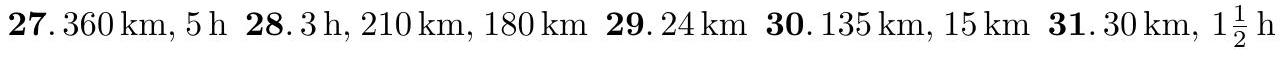
\includegraphics[max width=\textwidth, center]{2024_11_21_8f01584889ff06348ae7g-063}\\
32. a) 100\\
b) 10000\\
c) 1000000\\
d) 10000 e) 100 f) 10000\\
g) 100\\
h) 1000000\\
33. \(182120 \mathrm{~cm}^{2}\) 34. a) \(900 \mathrm{~cm}^{2}\), b) \(90000 \mathrm{~mm}^{2} \mathbf{3 5}\). a) 960 ha, b) 96000 arów \(\mathbf{3 6 .} 3200 \mathrm{~m}^{2}\)\\
37.13,5 ara\\
\(\mathbf{3 8 . 3 8} 869 \mathrm{zł}\)\\
39. a) \(1000 \mathrm{~mm}^{3}\) b) \(1000000 \mathrm{~mm}^{3}\) c) \(1000000 \mathrm{~cm}^{3}\)\\
d) \(1000000000 \mathrm{~m}^{3}\)\\
e) \(52000 \mathrm{~cm}^{3}\)\\
40.91 mm\\
\(41.45 \mathrm{zl} 42.96,76 \mathrm{~g}\)\\
\(43.143000 \mathrm{zł}\)\\
44. a) 0,04\\
b) 14600\\
c) 12000\\
d) 0,089\\
e) 0,103 f) 0,0044\\
g) \(90,2 \mathrm{~h}) 140 \mathrm{i})\)

125000 j) 0,038

\section*{Rozdział 3}
\section*{UKLAD WSPÓŁRZĘDNYCH}
Obecnie po raz pierwszy zapoznajemy się z układem współrzędnych na płaszczyźnie.\\
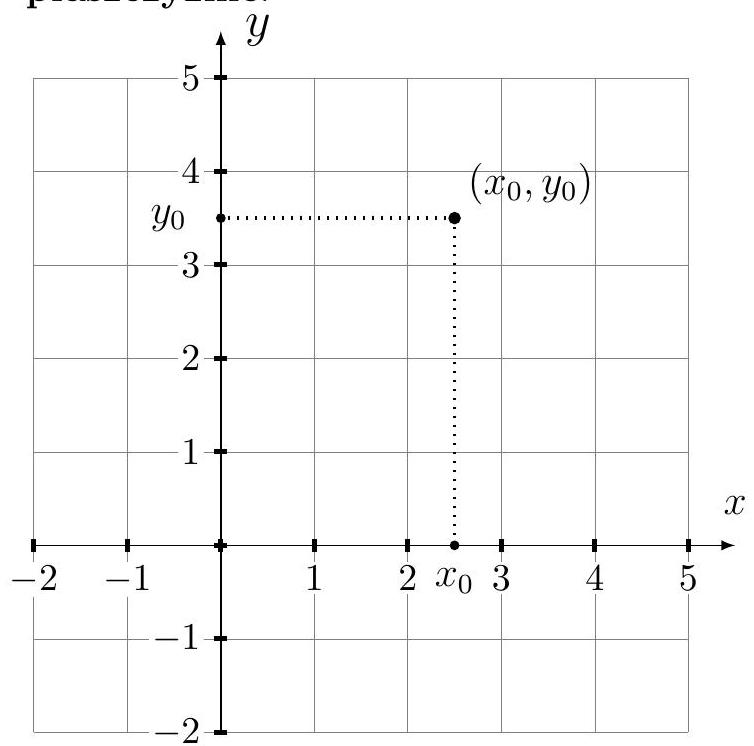
\includegraphics[max width=\textwidth, center]{2024_11_21_8f01584889ff06348ae7g-064}

Tworzą go dwie prostopadłe osie liczbowe przecinające się w punkcie odpowiadajacym liczbie 0 na obu osiach. Punkt ten oznaczamy literą \(O\), czy też cyfrą 0 , i nazywamy początkiem układu współrzędnych. Poziomą oś oznaczamy zazwyczaj literą \(x\), a pionową oś literą \(y\). Do tej pierwszej osi odwołujemy się najczęściej przez nazwę „oś \(O X "\), a do drugiej - „oś \(O Y "\). Na obu osiach obieramy zazwyczaj takie same jednostki.\\
Mając układ współrzędnych możemy opisywać położenie każdego punktu na płaszczyźnie przy pomocy pary liczb. Tę parę liczb nazywamy wówczas współrzędnymi tego punktu. Taką parę liczb będących współrzędnymi punktu zapisujemy następująco: \((7 ; 2),\left(4 \frac{1}{2} ; 5\right),(-2 ; 3)\), ogólnie \(\left(x_{0}, y_{0}\right)\).\\

\includegraphics[max width=\textwidth, center]{2024_11_21_8f01584889ff06348ae7g-065(1)}

\section*{UWAGA :}
Oś poziomą nazywa się częstokroć osia odciętych, a oś pionową osia rzędnych. Odpowiadające współrzędne punktu nazywamy wówczas odciętą i rzędną punktu.

\begin{enumerate}
  \item Narysuj układ współrzędnych przyjmując jedną kratkę za jednostkę, w taki sposób, żeby najmniejszą liczbą na osi poziomej było -3 , a największą 6, zaś na osi pionowej najmniejszą liczbą -4, a największą 6. Następnie zaznacz w tym układzie kolejno podane poniżej punkty, łącząc je kolejno odcinkami.
\end{enumerate}

\begin{center}
\begin{tabular}{lllllll}
1. \(\quad(-2,6)\) & 2. \(\quad(-2,3)\) & 3. \((-1,2)\) & 4. \(\cdot(-2,1)\) & 5. \(\cdot(-3,-1)\) \\
6. \((-3,-3)\) & 7. \((-2,-4)\) & 8. \((1,-4)\) & 9. \((4,-2)\) & 10. \((4,1)\) \\
11. \((6,2)\) & 12. \((6,3)\) & 13. \((4,3)\) & 14. \((3,2)\) & 15. \((3,-1)\) \\
16. \((2,-2)\) & 17. \((2,-1)\) & 18. \((1,1)\) & 19. \((0,2)\) & 20. \((1,3)\) \\
21. \((1,6)\) & 22. \((0,5)\) & 23. \((-1,5)\) & 24. \((-2,6)\) &  \\
\end{tabular}
\end{center}

Osie układu współrzędnych dzielą płaszczyznę na cztery części zwane ćwiartkami, które zwyczajowo są numerowane tak jak na rysunku obok. Zauważ, że

\begin{itemize}
  \item punkty, które leżą w I ćwiartce płaszczyzny mają obie współrzędne dodatnie
  \item punkty, które leżą w drugiej ćwiartce płaszczyzny, mają pierwszą współrzędną \(x\) ujemną, a drugą współrzędną \(y\) dodatnią, itd.
  \item punkty, które leżą na osi poziomej (czyli OX) mają drugą współrzędną równą 0, a punkty które leżą na osi pionowej czyli OY mają pierwszą współrzędną równa 0.\\
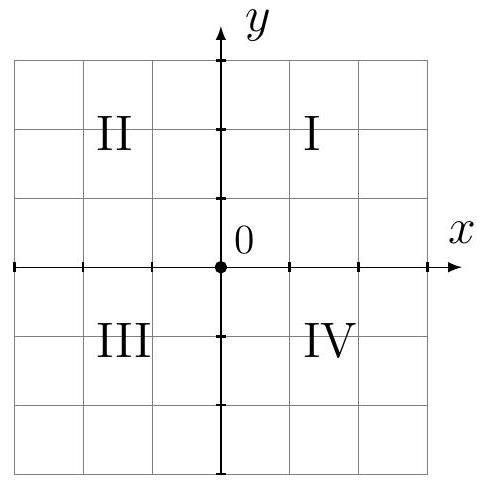
\includegraphics[max width=\textwidth, center]{2024_11_21_8f01584889ff06348ae7g-065}
\end{itemize}

\begin{enumerate}
  \setcounter{enumi}{1}
  \item W układzie współrzędnych zaznacz pięć punktów takich, że pierwsza i druga współrzędna są równe a przy tym są one liczbami całkowitymi.
  \item W układzie współrzędnych zaznacz 5 punktów, w których druga współrzędna jest równa \(1 \frac{1}{2}\), zaś pierwsza współrzędna jest liczbą całkowitą.
  \item W tym zadaniu do każdego podpunktu rób oddzielny rysunek przyjmując jako jednostkę 2 kratki. Zaznacz 6 punktów o pierwszej współrzędnej równej 2, a przy tym druga współrzędna jest\\
a) dodatnia, ale mniejsza od 5;\\
b) ujemna, ale większa od -4 ;\\
c) większa od -4 , ale mniejsza od 2 ;\\
d) nieujemna, ale mniejsza od 5;\\
e) niecałkowita, a przy tym większa od -2 a mniejsza od 2 .
  \item Tu też do każdego podpunktu rób osobny rysunek. W układzie współrzędnych zaznacz 6 punktów o drugiej współrzędnej równej 3, a przy tym pierwsza współrzędna jest\\
a) dodatnia, ale mniejsza od 4;\\
b) ujemna, ale większa od -3 ;\\
c) większa od -3 , ale mniejsza od 2 ;\\
d) nieujemna, ale mniejsza od 4;\\
e) niecałkowita, a przy tym większa od -2 a mniejsza od 2 .
  \item W tym zadaniu do każdego podpunktu rób oddzielny rysunek przyjmując 1 kratkę jako 1 jednostkę. W układzie współrzędnych zaznacz te wszystkie punkty, których\\
a) pierwsza współrzędna jest równa 1 ,\\
b) pierwsza współrzędna jest równa -2 ,\\
c) druga współrzędna jest równa 2,\\
d) druga współrzędna jest równa 0 ,\\
e) obie współrzędne są sobie równe.
  \item Do każdego podpunktu rób oddzielny rysunek przyjmując 1 kratkę jako 1 jednostkę. Zaznacz w układzie współrzędnych zbiór tych wszystkich punktów, których współrzędne spełniają następujące warunki:\\
a) pierwsza współrzędna jest dodatnia,\\
b) druga współrzędna jest ujemna,\\
c) obie współrzędne są dodatnie,\\
d) obie współrzędne są ujemne,\\
e) pierwsza współrzędna jest większa niż 2,\\
f) druga współrzędna jest mniejsza od 3,\\
g) współrzędne punktu są liczbami przeciwnymi,\\
h) druga współrzędna jest nie mniejsza od 2.
  \item Zaznacz w układzie współrzędnych zbiór tych wszystkich punktów, których współrzędne spełniają następujące warunki:\\
a) pierwsza współrzędna jest równa 2, a druga większa lub równa 3,\\
b) pierwsza współrzędna jest równa 1, a druga większa od -1 ,\\
c) pierwsza współrzędna jest równa 3, a druga jest większa lub równa 3,\\
d) pierwsza współrzędna jest równa 4, a druga jest mniejsza lub równa 4,\\
e) pierwsza współrzędna jest równa 2, a druga jest większa od pierwszej współrzędnej,\\
f) pierwsza współrzędna jest równa 1, a druga jest mniejsza od pierwszej współrzędnej,\\
g) druga współrzędna jest równa pierwszej współrzędnej,\\
h) druga współrzędna jest większa od pierwszej współrzędnej;\\
i) druga współrzędna jest mniejsza od pierwszej współrzędnej;\\
j) pierwsza współrzędna jest większa od drugiej współrzędnej;\\
k) druga współrzędna jest o 1 większa od pierwszej współrzędnej.
  \item Zaznacz na płaszczyźnie z układem współrzędnych zbiór tych wszystkich punktów, których współrzędne \((x, y)\) spełniają warunek (warunki):\\
(1) \(x=1\)\\
(2) \(x=0\)\\
(3) \(y=-2\)\\
(4) \(y=0\)\\
(5) \(x \geqslant 0\)\\
(6) \(x \leqslant 2\)\\
(7) \(y \geqslant 0\)\\
(8) \(y \geqslant 3\)\\
(9) \(0 \leqslant x \leqslant 3\)\\
(10) \(-1 \leqslant y \leqslant 2\)\\
(11) \(-2 \leqslant x \leqslant 2\) i \(-1 \leqslant y \leqslant 1\)\\
(12) \(\left\{\begin{array}{l}x \geqslant 0 \\ y \geqslant 0\end{array}\right.\)\\
(13) \(\left\{\begin{array}{l}x \geqslant 1 \\ y \geqslant 2\end{array}\right.\)\\
(14) \(\left\{\begin{array}{l}x \leqslant 0 \\ y \leqslant 3\end{array}\right.\)\\
(15) \(\left\{\begin{array}{l}0 \leqslant x \leqslant 2 \\ y=x\end{array}\right.\)\\
(16) \(\left\{\begin{array}{l}x=-1 \\ y \leqslant 2\end{array}\right.\)\\
(17) \(\left\{\begin{array}{l}y=-2 \\ x>-1\end{array}\right.\)\\
(18) \(\left\{\begin{array}{l}y=1 \\ x \geqslant 3\end{array}\right.\)\\
(19) \(\left\{\begin{array}{l}0 \leqslant x \leqslant 3 \\ y \leqslant 2\end{array}\right.\)\\
(20) \(\left\{\begin{array}{l}-1 \leqslant x \leqslant 2 \\ y \geqslant 0\end{array}\right.\)\\
(21) \(\left\{\begin{array}{l}x=1 \\ y \geqslant 3\end{array}\right.\)\\
(22) \(\left\{\begin{array}{l}y=x \\ x \in \mathbb{Z}\end{array}\right.\)\\
(23) \(\left\{\begin{array}{l}-1<y \leqslant 3 \\ x \in \mathbb{Z}\end{array}\right.\)\\
(24) \(\left\{\begin{array}{l}x-y=0 \\ y>-1\end{array}\right.\)\\
(25) \(\left\{\begin{array}{l}y=-2 \\ x \geqslant-1\end{array}\right.\)\\
(26) \(\left\{\begin{array}{l}x>0 \\ y \in \mathbb{Z}\end{array}\right.\)\\
(27) \(\left\{\begin{array}{l}x \in\{-1,1\} \\ y \leqslant 1\end{array}\right.\)\\
(28) \(\left\{\begin{array}{l}x>y \\ y \geqslant 0\end{array}\right.\)\\
(29) \(\left\{\begin{array}{l}x \leqslant 3 \\ |y|=2\end{array}\right.\)\\
(30) \(\left\{\begin{array}{l}y \leqslant x \\ y \geqslant-x\end{array}\right.\)\\
(31) \(\left\{\begin{array}{l}x \leqslant y \\ -2 \geqslant x \leqslant 2\end{array}\right.\)\\
(32) \(\left\{\begin{array}{l}|x| \leqslant 2 \\ |y|<2\end{array}\right.\)\\
(33) \(\left\{\begin{array}{l}|x|>3 \\ |y|>1\end{array}\right.\)\\
(34) \(\left\{\begin{array}{l}y=|x| \\ |x|<2 \\ y>1\end{array}\right.\)\\
(35) \(\left\{\begin{array}{l}y>|x| \\ |x| \geqslant 1\end{array}\right.\)
  \item Opisz za pomocą odpowiednich warunków dla \(x, y\) następujące zbiory punktów:\\
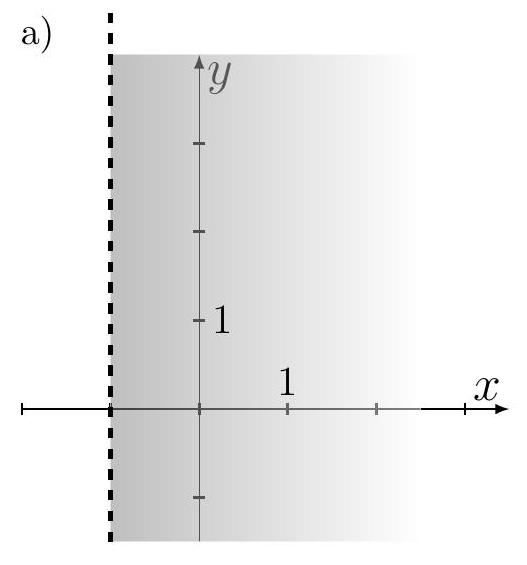
\includegraphics[max width=\textwidth, center]{2024_11_21_8f01584889ff06348ae7g-068(3)}\\
b)\\
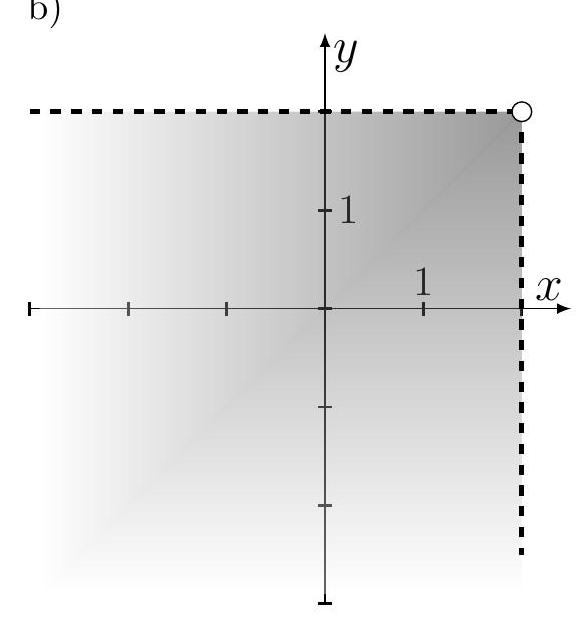
\includegraphics[max width=\textwidth, center]{2024_11_21_8f01584889ff06348ae7g-068(1)}\\
c)\\
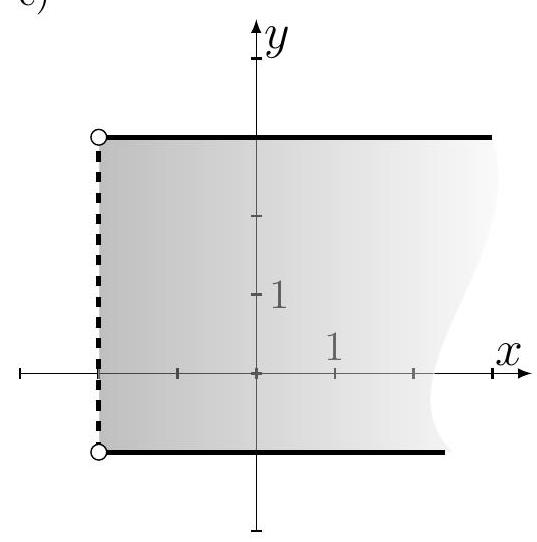
\includegraphics[max width=\textwidth, center]{2024_11_21_8f01584889ff06348ae7g-068}\\
d)\\
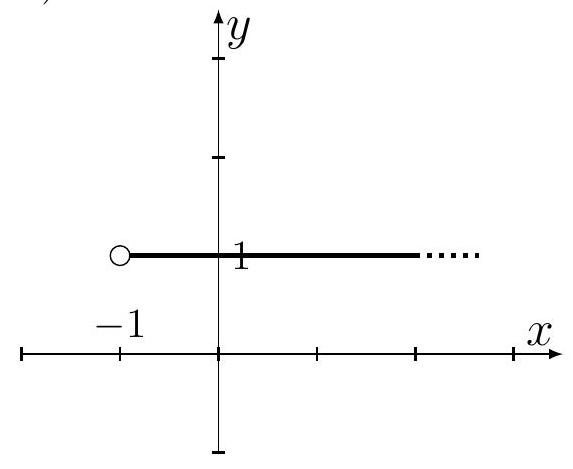
\includegraphics[max width=\textwidth, center]{2024_11_21_8f01584889ff06348ae7g-068(2)}\\
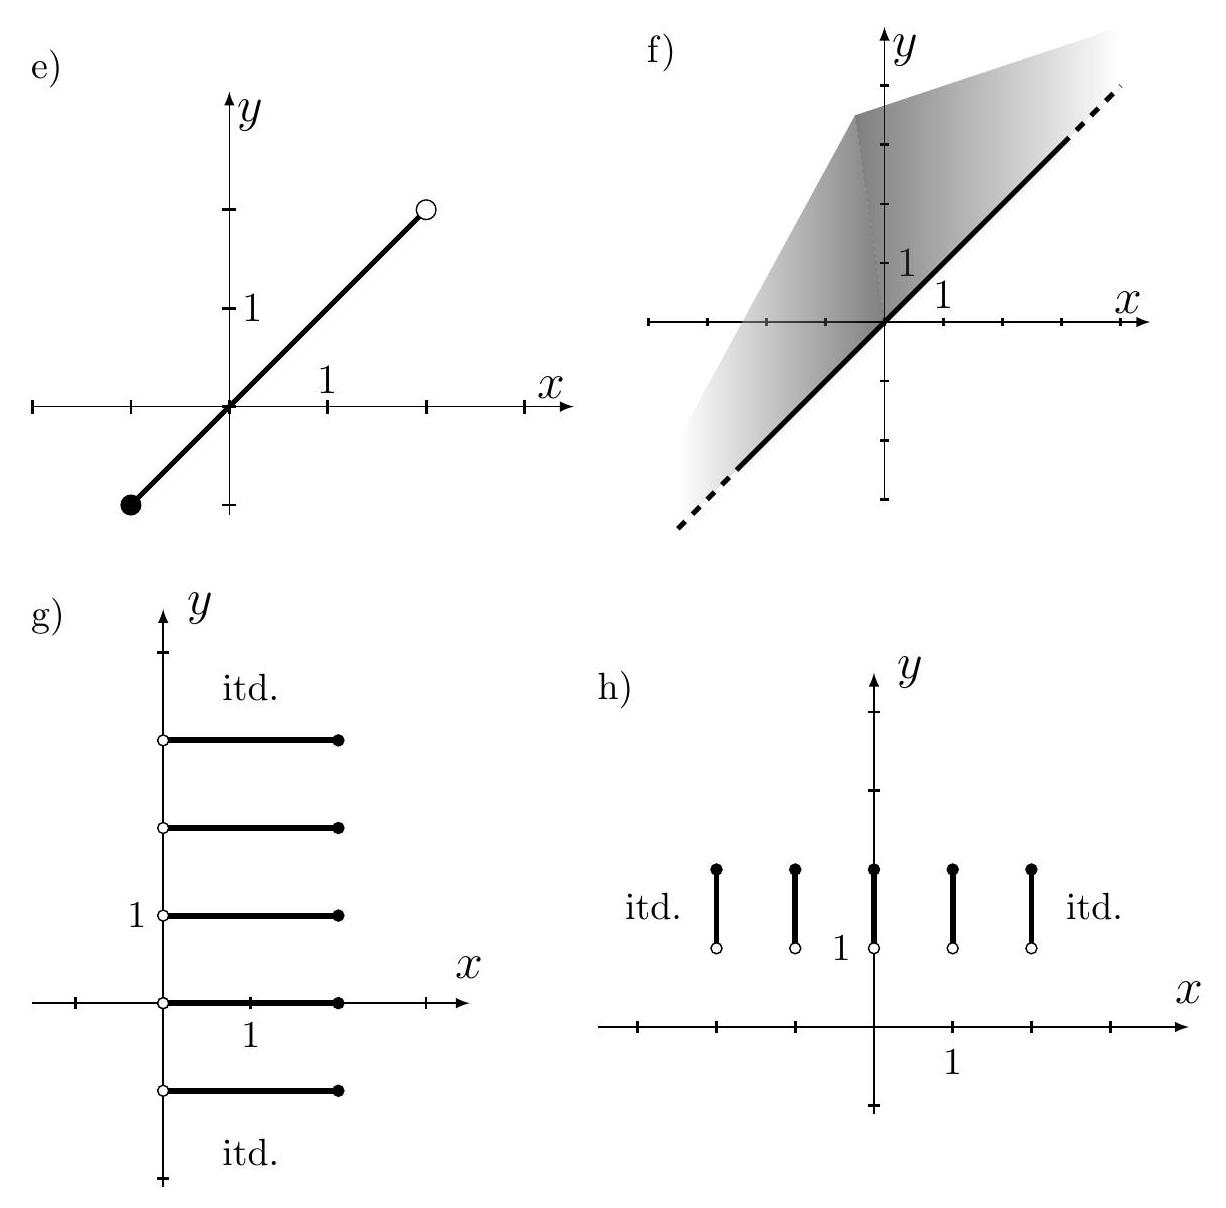
\includegraphics[max width=\textwidth, center]{2024_11_21_8f01584889ff06348ae7g-069(2)}\\
j)\\
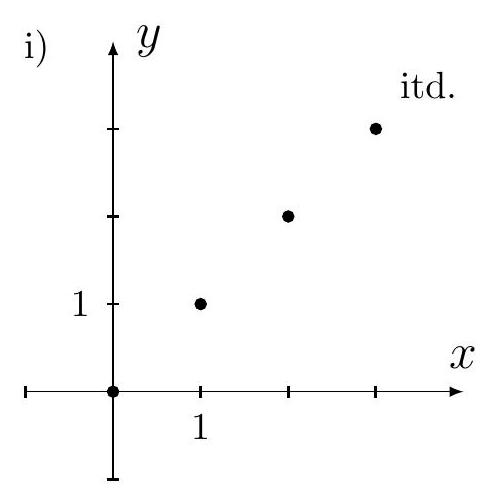
\includegraphics[max width=\textwidth, center]{2024_11_21_8f01584889ff06348ae7g-069}\\
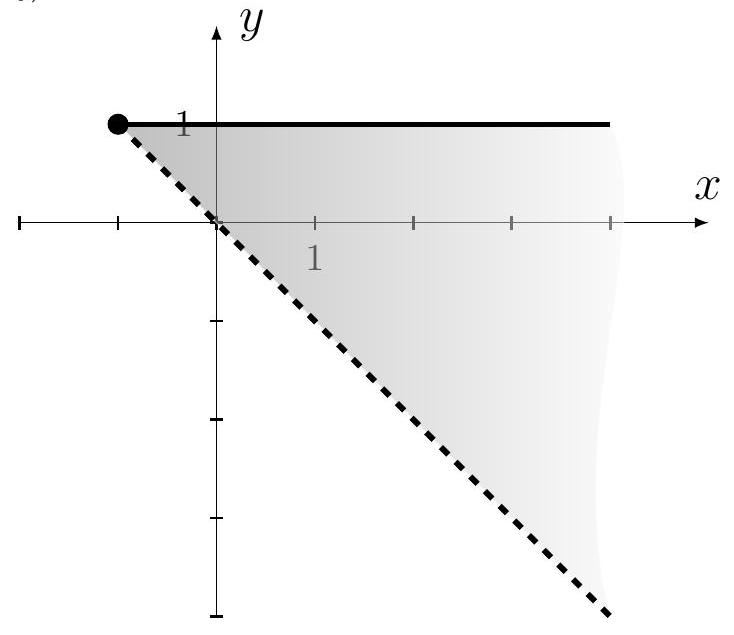
\includegraphics[max width=\textwidth, center]{2024_11_21_8f01584889ff06348ae7g-069(1)}\\
k)\\
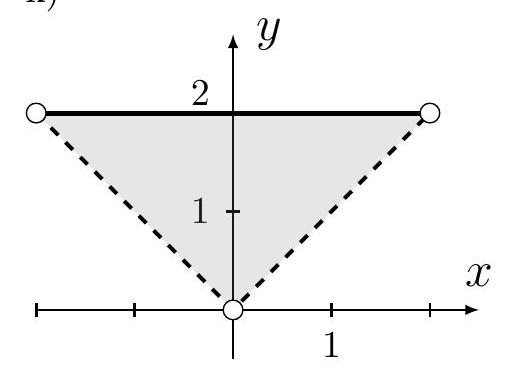
\includegraphics[max width=\textwidth, center]{2024_11_21_8f01584889ff06348ae7g-070}\\
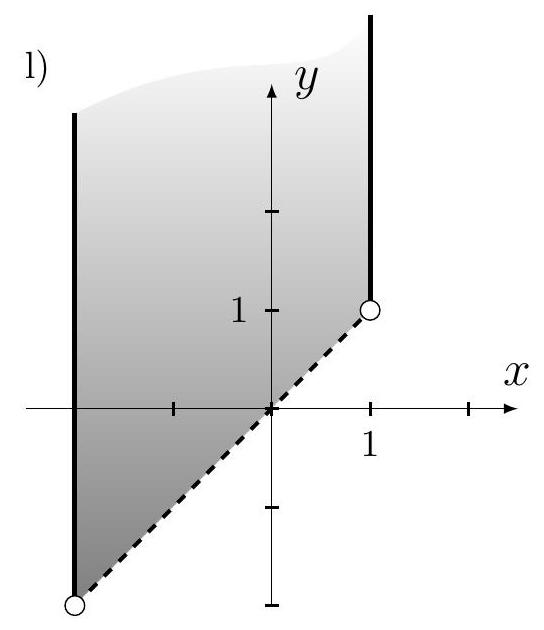
\includegraphics[max width=\textwidth, center]{2024_11_21_8f01584889ff06348ae7g-070(2)}\\
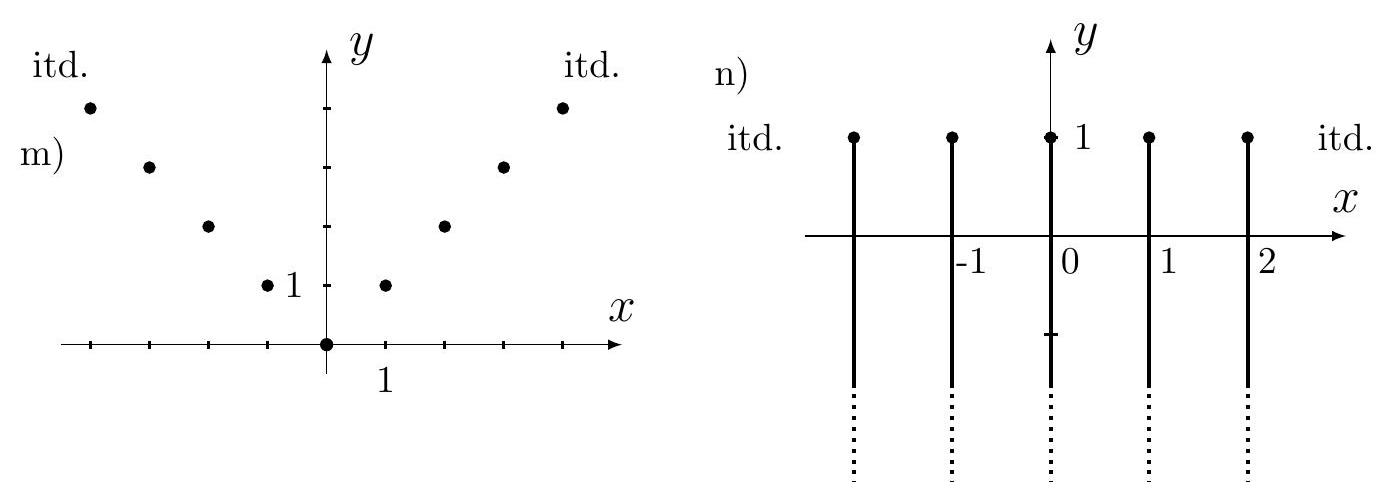
\includegraphics[max width=\textwidth, center]{2024_11_21_8f01584889ff06348ae7g-070(3)}\\
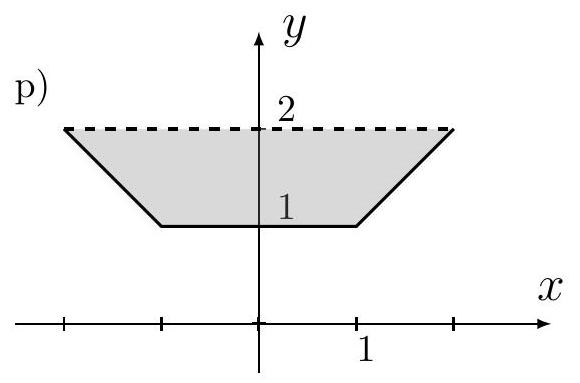
\includegraphics[max width=\textwidth, center]{2024_11_21_8f01584889ff06348ae7g-070(1)}\\
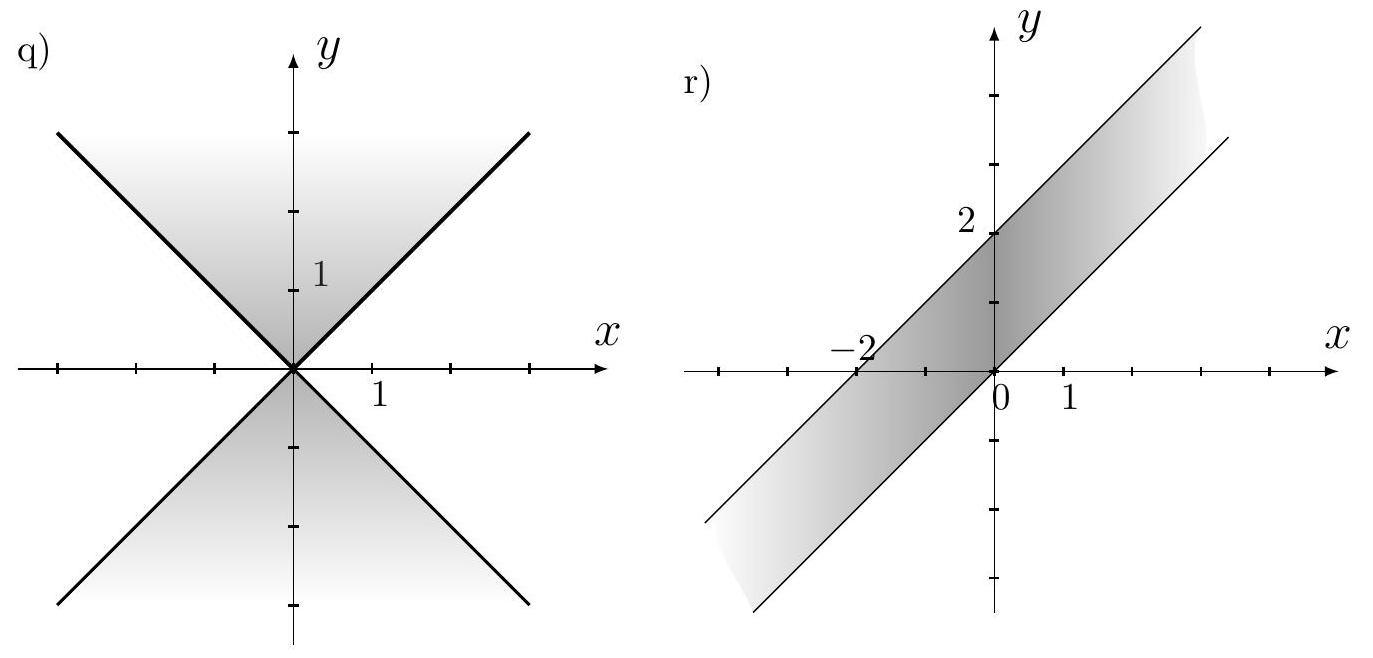
\includegraphics[max width=\textwidth, center]{2024_11_21_8f01584889ff06348ae7g-071(1)}
\end{enumerate}

WYKRESY\\
Z układem współrzędnych związane jest pojęcie wykresu zależności jednej wielkości od drugiej.\\
11. Poniższy wykres przedstawia jak w pewnym miejscu w czasie 24 godzin zmieniała się temperatura powietrza. Odczytaj z wykresu:\\
a) O której godzinie temperatura była najniższa?\\
b) O której godzinie temperatura była najwyższa?\\
c) W których godzinach temperatura wzrastała?\\
d) Ile razy w ciągu tych 24 godzin temperatura wynosiła \(15^{\circ}\) ?\\
e) Ile razy w ciągu tych 24 godzin temperatura wynosiła \(17^{\circ}\) ?\\
f) W którym czasie temperatura nie przekraczała \(10^{\circ}\) ?\\
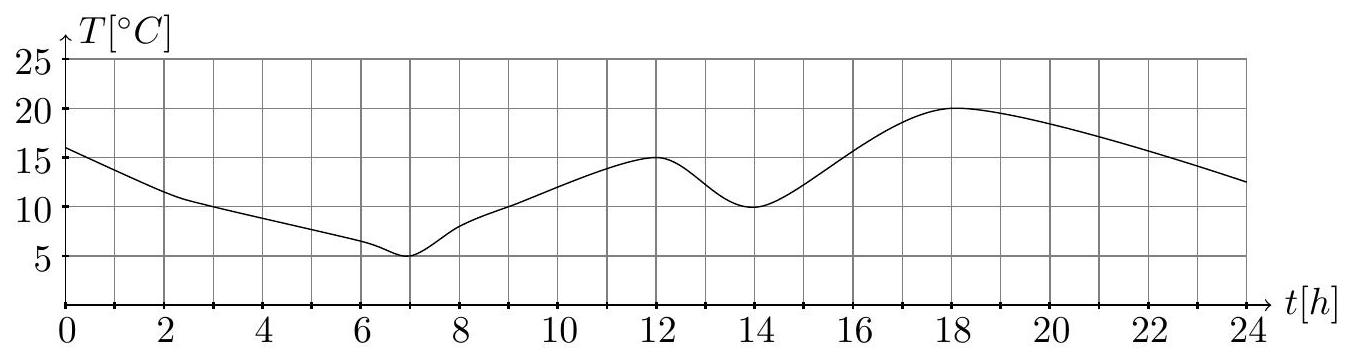
\includegraphics[max width=\textwidth, center]{2024_11_21_8f01584889ff06348ae7g-071}\\
12. Na poniższym wykresie widać jak zmieniała się w pewnym miejscu w ciągu doby temperatura powietrza. Odczytaj z wykresu:\\
a) Jaka była najniższa temperatura w ciągu tych 24 godzin?\\
b) O której godzinie temperatura była najwyższa? Ile było stopni ciepła?\\
c) W których godzinach temperatura opadała?\\
d) W jakim czasie temperatura wynosiła \(4^{\circ}\) ?\\
e) W którym czasie temperatura była wyższa niż \(6^{\circ}\) ?\\
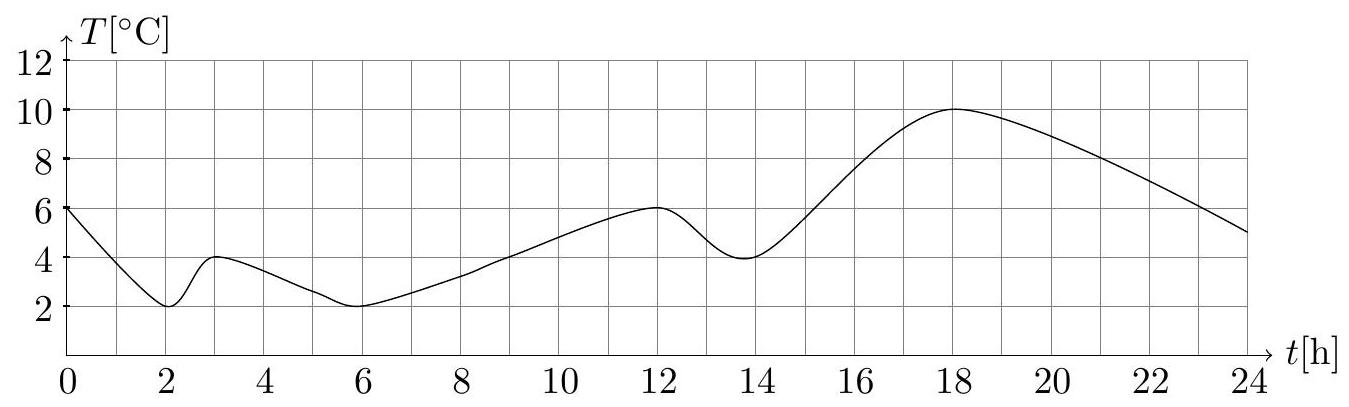
\includegraphics[max width=\textwidth, center]{2024_11_21_8f01584889ff06348ae7g-072}

Przy sporządzaniu wykresów w układzie współrzędnych nie musimy rysować siatki, ale dorysowanie siatki ułatwia nam odczytywanie wykresu.\\
13. Wykres obok przedstawia jak zmieniała się ilość benzyny w baku w czasie jazdy samochodu ze stałą prędkością.\\
a) Po ilu kilometrach w baku było 20 litrów benzyny?\\
b) Ile litrów benzyny spalał samochód na dystansie 100 km?\\
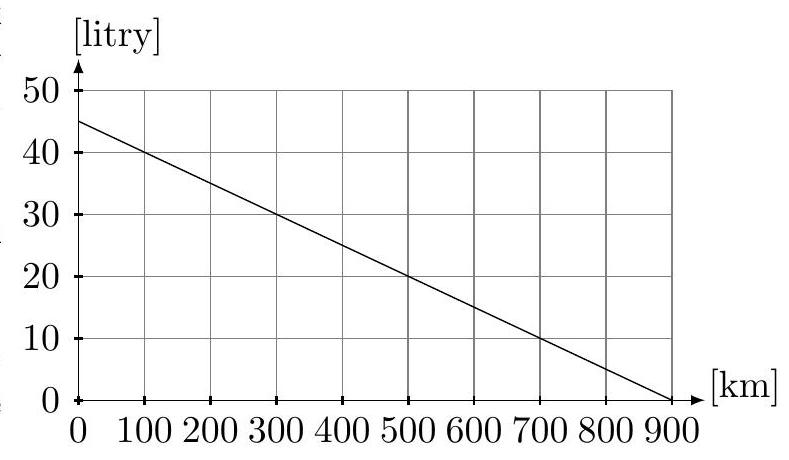
\includegraphics[max width=\textwidth, center]{2024_11_21_8f01584889ff06348ae7g-072(1)}\\
14. Do czajnika wlano wpierw wodę z kranu, potem zaczęto go podgrzewać, a po zagotowaniu wody wyłączyło się podgrzewanie. Poniższy wykres przedstawia jak zmieniała się temperatura wody w czajniku.\\
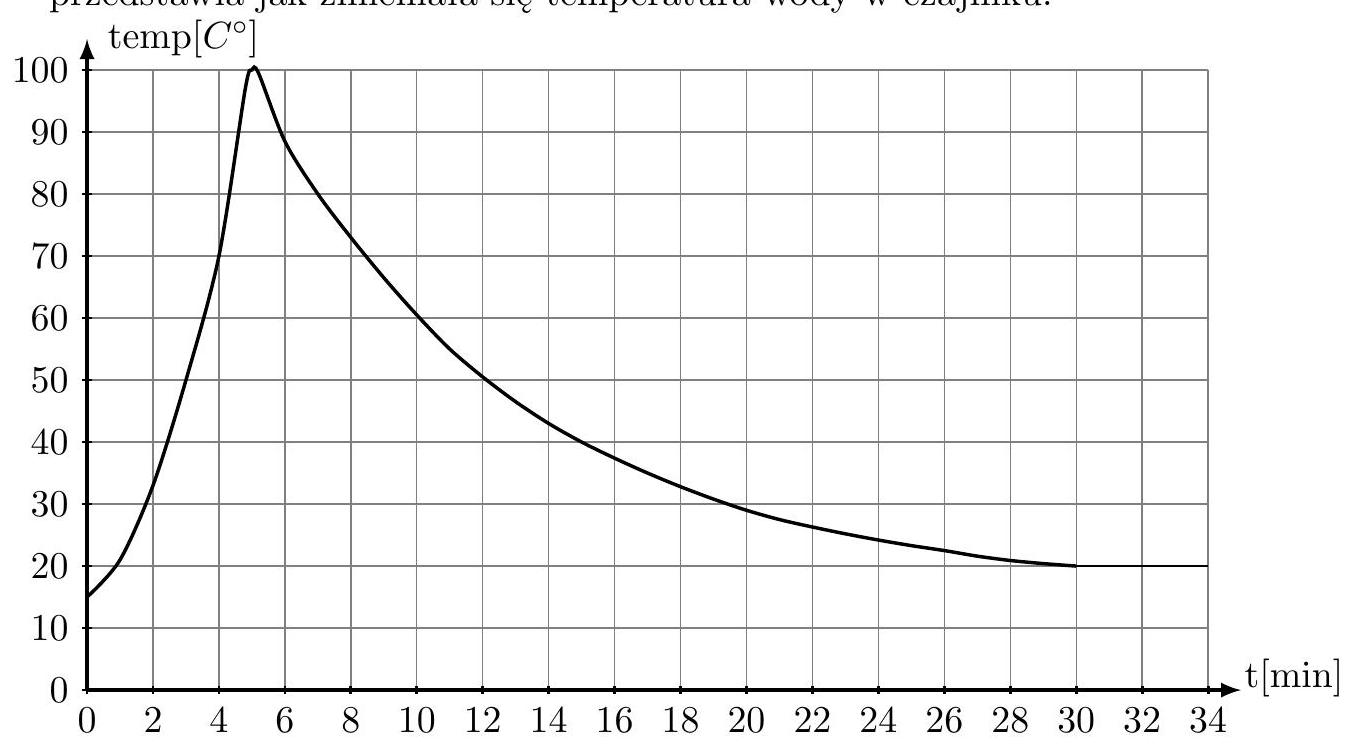
\includegraphics[max width=\textwidth, center]{2024_11_21_8f01584889ff06348ae7g-073(1)}

Na podstawie tego wykresu odpowiedz na pytania:\\
a) Jaka była temperatura wody w kranie?\\
b) Jak długo woda była podgrzewana?\\
c) Po ilu minutach woda osiągnęła temperaturę 30 stopni?\\
d) Po ilu kolejnych minutach temperatura ponownie spadła do \(30^{\circ}\) ?\\
e) Jaka była temperatura pomieszczenia w którym znajdował się czajnik?\\
15. Wykres poniższy przedstawia jak zmieniała się liczba kilometrów, którą przejechał rowerzysta w czasie 3 godzin.\\
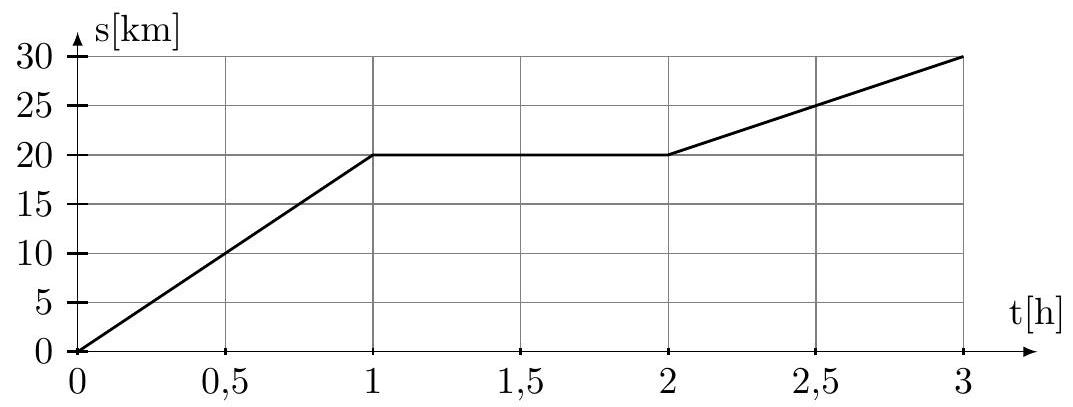
\includegraphics[max width=\textwidth, center]{2024_11_21_8f01584889ff06348ae7g-073}

Na podstawie wykresu oceń\\
a) Po jakim czasie rowerzysta przejechał 15 kilometrów?\\
b) Ile kilometrów przebył on po \(1 \frac{1}{2}\) godziny?\\
c) Jak długo trwała przerwa w podróży?\\
d) Z jaką prędkością jechał on w pierwszej, a z jaką w trzeciej godzinie?\\
16. Samochód jechał cały czas z tą samą prędkością. Wykres przedstawia ilość przejechanych kilometrów. Ile kilometrów przejechał samochód w ciągu \(2 \frac{1}{2}\) godziny?\\
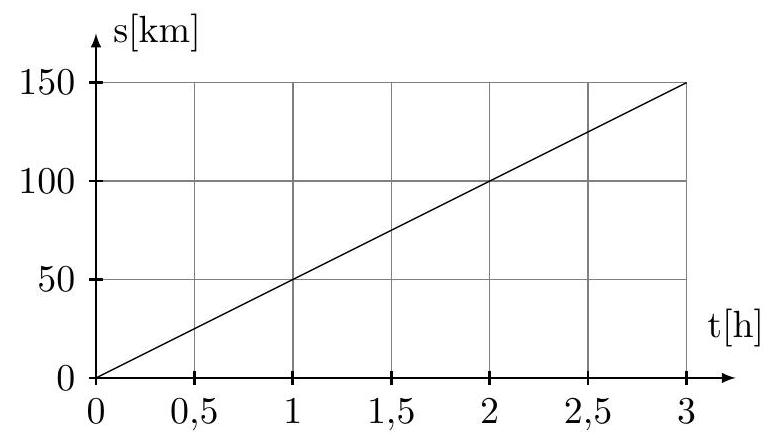
\includegraphics[max width=\textwidth, center]{2024_11_21_8f01584889ff06348ae7g-074(1)}\\
17. W baku było na początku 50 litrów benzyny. Wykres obok przedstawia ilość spalonej benzyny w zależności od ilości przejechanych kilometrów.\\
a) Ile litrów benzyny spalał samochód na dystansie 100 km ?\\
b) Po ilu kilometrach w baku było 20 litrów benzyny?\\
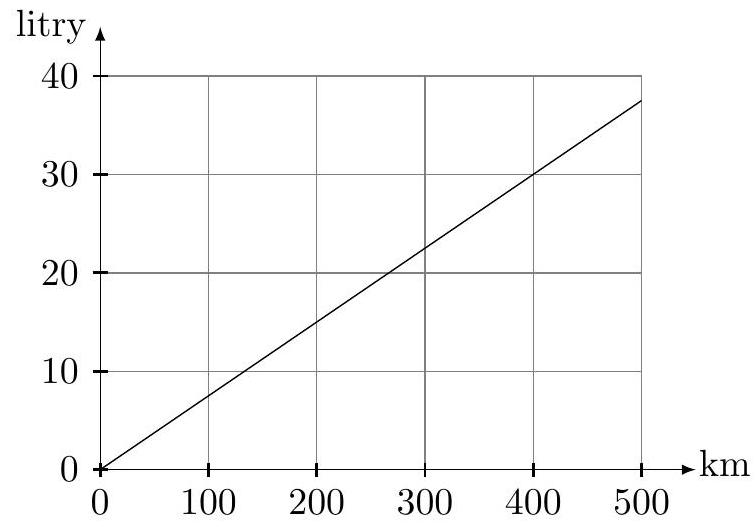
\includegraphics[max width=\textwidth, center]{2024_11_21_8f01584889ff06348ae7g-074}

Ostatnie dwa wykresy są wykresami tzw. proporcjonalności prostej. Mówimy, na przykład, że w ruchu jednostajnym ilość przejechanych kilometrów jest wprost proporcjonalna do ilości spalonej benzyny. Poniżej mamy dalsze przykłady wielkości wprost proporcjonalnych.\\
(I.) Długość siatki ogrodzeniowej i jej koszt.

Jeżeli 1 metr siatki ogrodzeniowej kosztuje 35 zł, to za 3 metry siatki zapłacimy 3 razy więcej czyli 105 zł za 3,5 metra siatki zapłacimy \(3,5 \cdot 35=122,5 \mathrm{zł}\) za 2,2 metra siatki zapłacimy \(77 \mathrm{zł}\)\\
Zależność pomiędzy długością kupowanej siatki a jej kosztem przedstawia poniższy wykres\\
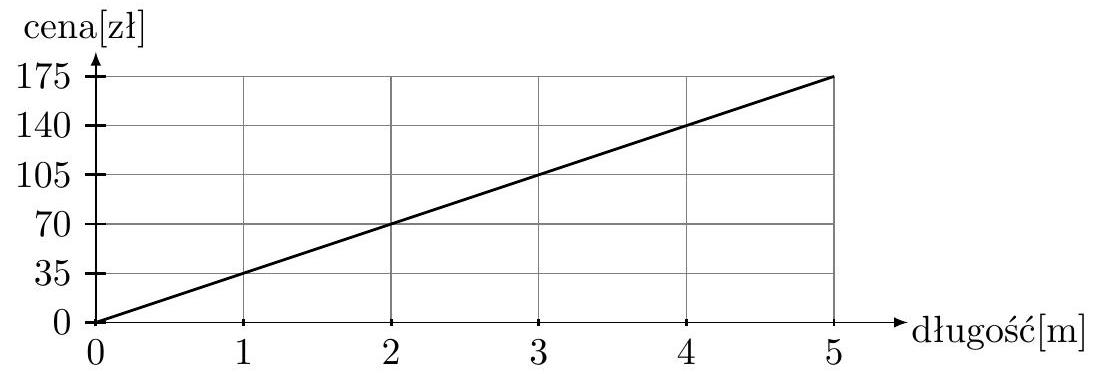
\includegraphics[max width=\textwidth, center]{2024_11_21_8f01584889ff06348ae7g-075(1)}\\
(II.) Objętość śmietany i jej masa.

\begin{center}
\begin{tabular}{c|c|c|c|c|c}
objętość śmietany & 200 ml & 100 ml & 50 ml & 250 ml & 1 ml \\
\hline
masa śmietany & 260 g & 130 g & 65 g & 325 g & \(1,3 \mathrm{~g}\) \\
\hline
\end{tabular}
\end{center}

Zależność pomiędzy tymi dwiema wielkościami przedstawia wykres masa[g]\\
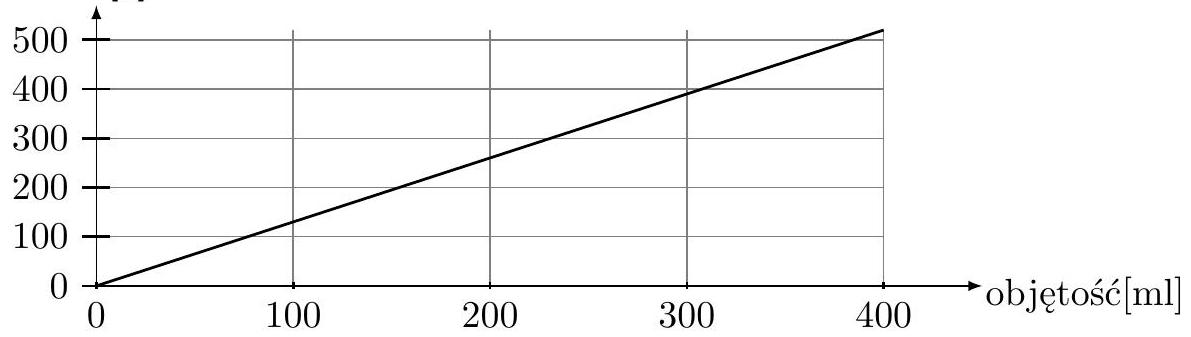
\includegraphics[max width=\textwidth, center]{2024_11_21_8f01584889ff06348ae7g-075}\\
(III.) Odległość na mapie i odpowiadającą jej odległość w terenie.

\begin{center}
\begin{tabular}{c|c|c|c|c|c}
odległość na mapie & 1 cm & 2 cm & 4 cm & 5 cm & \(0,5 \mathrm{~cm}\) \\
\hline
odległość w terenie & 150 m & 300 m & 600 m & 750 m & 75 m \\
\hline
\end{tabular}
\end{center}

Sporządź wykres tej zależności w poniższym układzie współrzędnych w terenie [m]\\
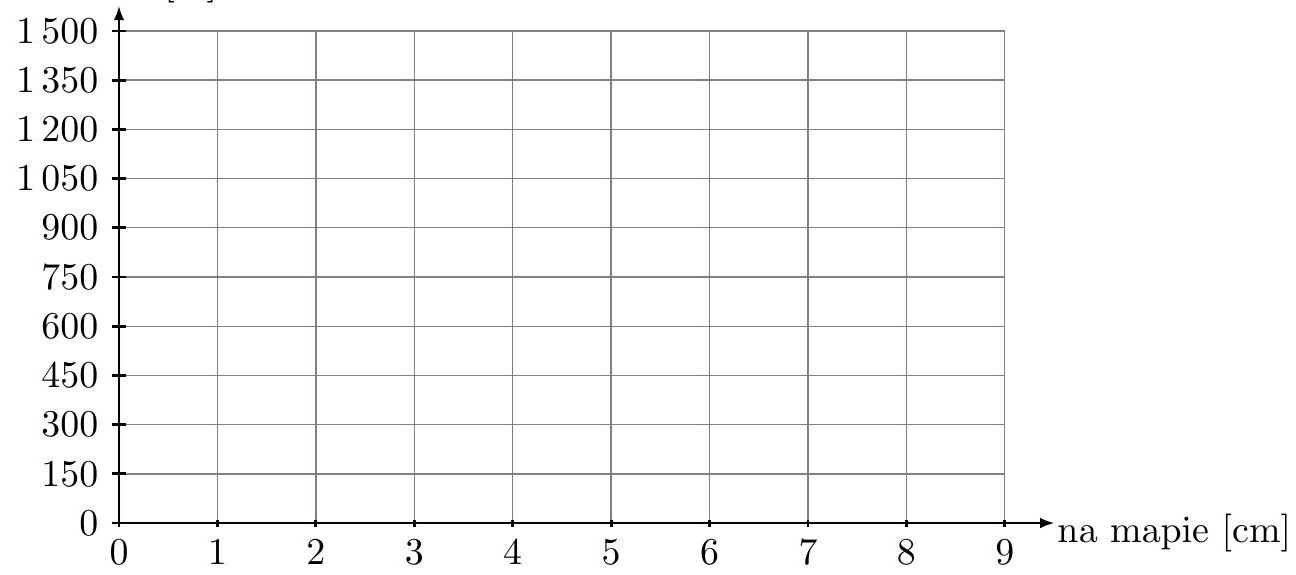
\includegraphics[max width=\textwidth, center]{2024_11_21_8f01584889ff06348ae7g-076(1)}

Ze sporządzonego wykresu odczytaj\\
a) Jaka odległość w terenie odpowiada odległości \(4,5 \mathrm{~cm}\) na mapie?\\
b) Jakiej odległości na mapie odpowiada odległość 480 m w terenie?\\
(IV.) Ilość (jednakowych) zeszytów i suma jaką trzeba za nie zapłacić.

\begin{center}
\begin{tabular}{c|c|c|c|c|c}
ilość zeszytów & 1 & 2 & 3 & 4 & 5 \\
\hline
koszt & \(1,20 \mathrm{zł}\) & \(2,40 \mathrm{zł}\) & \(3,60 \mathrm{zł}\) & \(4,80 \mathrm{zł}\) & \(6 \mathrm{zł}\) \\
\hline
\end{tabular}
\end{center}

koszt [zl]\\
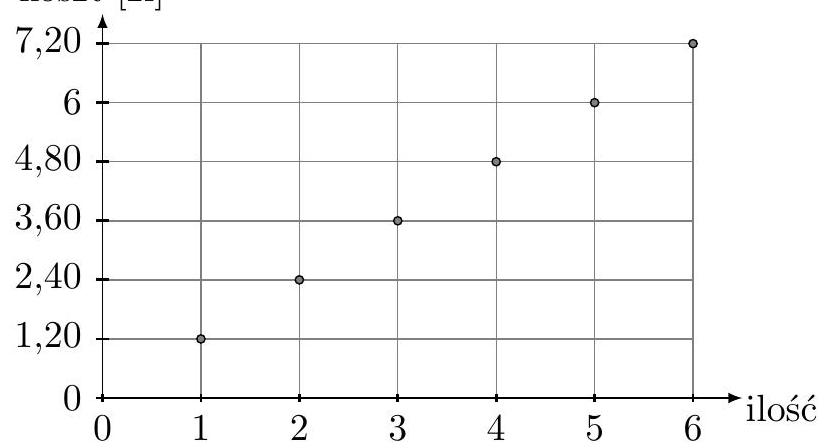
\includegraphics[max width=\textwidth, center]{2024_11_21_8f01584889ff06348ae7g-076}

Dwie wielkości są wprost proporcjonalne, gdy wzrastanie/zmniejszanie się jednej wielkości wiąże się z wzrastaniem/zmniejszaniem się tyle samo razy drugiej wielkości.\\
Zauważ, że we wszystkich podanych przykładach iloraz wielkości proporcjonalnych jest stały:

\begin{enumerate}
  \item \(\frac{35 \mathrm{zł}}{1 \mathrm{~m}}=\frac{70 \mathrm{zł}}{2 \mathrm{~m}}=\frac{105 \mathrm{zł}}{3 \mathrm{~m}}=\frac{122,5 \mathrm{zł}}{3,5 \mathrm{~m}}=\frac{77 \mathrm{zł}}{2,2 \mathrm{~m}}=35 \mathrm{zł} / \mathrm{m}-\) tu ten iloraz wyraża cenę 1 metra siatki.
  \item \(\frac{260 \mathrm{~g}}{200 \mathrm{~cm}^{3}}=\frac{130 \mathrm{~g}}{100 \mathrm{~cm}^{3}}=\frac{65 \mathrm{~g}}{50 \mathrm{~cm}^{3}}=\frac{325 \mathrm{~g}}{250 \mathrm{~cm}^{3}}=\frac{1,3}{1 \mathrm{~cm}^{3}}=1,3 \mathrm{~g} / \mathrm{cm}^{3}-\) to nazywamy gęstością śmietany
  \item \(\frac{1 \mathrm{~cm}}{15000 \mathrm{~cm}}=\frac{2 \mathrm{~cm}}{30000 \mathrm{~cm}}=\frac{5 \mathrm{~cm}}{75000 \mathrm{~cm}}=\frac{0,5 \mathrm{~cm}}{7500 \mathrm{~cm}}=\frac{1}{15000}\)
\end{enumerate}

Tę wielkość zapisujemy zazwyczaj w postaci 1 : 15000 i nazywamy skala mapy.\\
Te ilorazy, o których jest mowa w powyższych przykładach, nazywamy zazwyczaj wspótczynnikiem proporcjonalności.\\
18. W poniższych pytaniach mamy do czynienia z proporcjonalnością prostą. W miejsce kropek wpisz odpowiedzi.\\
a) Jeżeli 12 biletów kosztuje \(30 \mathrm{zł}\), to z tego wynika, że 8 biletów kosztuje ........ zł.\\
b) Jeżeli 5 zeszytów kosztuje 11 zł, to z tego wynika, że 3 zeszyty kosztują ........ zł.\\
c) Jeżeli samochód w ciągu 4 godzin przejechał 300 km , to z tego wynika, że w ciągu 1,5 godziny przejedzie on \(\ldots \ldots . . \mathrm{km}\).\\
d) Jeżeli na 600 km samochód spala 33 litry benzyny, to z tego wynika, że na 250 km spala on ....... litrów benzyny.\\
e) Jeżeli 150 gram grzybów kosztuje 6 zł, to z tego wynika że 400 gram kosztuje ........ zł.\\
f) Jeżeli 750 gram grzybów kosztuje 12 zł, to 250 gram kosztuje ..... zł.\\
g) Jeżeli 250 gram czekolady ma wartość energetyczną 320 kcal, to 100 gram ma wartość energetyczną ........ kcal.\\
19. Pociąg jechał ze stałą prędkością. W czasie 4 minut i 30 sekund przejechał on \(3,6 \mathrm{~km}\).\\
a) Ile kilometrów przejedzie on w czasie 13 minut i 30 sekund?\\
b) W jakim czasie przejedzie on 18 kilometrów?\\
c) Ile metrów przejeżdża ten pociąg w ciągu minuty?\\
d) Ile kilometrów przejeżdża ten pociąg w ciągu 1 godziny?\\
20. Pusta mała beczka o pojemności 20 litrów waży 3 kg , a pusta duża beczka o pojemności 50 litrów waży 5 kg . Mała beczka wypełniona smołą waży 25 kg . Ile będzie ważyła duża beczka po wypełnieniu jej smołą?\\
21. Asia w czasie konkursu na szybkość pisania na klawiaturze napisała w pewnym czasie 4920 znaków. Gdyby pisała o 5 znaków na minutę więcej, to napisałaby w tym samym czasie 5040 znaków. Ile znaków na minutę pisała zatem Asia?

Do roku 1971 w Wielkiej Brytanii w obiegu pieniężnym były następujące jednostki pieniężne: funty, szylingi i pensy. Przy czym

1 funt \(=20\) szylingów\\
1 szyling \(=12\) pensów czyli

1 funt \(=240\) pensów.\\
22. (aut. John Mellis 1594 r) Jeżeli 1 jard sukna kupujesz za 6 szylingów i 8 pensów, a sprzedajesz za 8 szylingów i 6 pensów, to ile zarobisz na każdych 100 szylingach zainwestowanych w taką transakcję?

\section*{Rozdział 4}
\section*{POTĘGI I JEDNOMIANY}
Przypomnijmy wpierw, że potęga jest to skrócony zapis iloczynu pewnej ilości takich samych czynników:\\
\(a^{n}=\underbrace{a \cdot a \cdot \ldots \cdot a}_{n-\text { czynników }} \quad\) dla \(n \geqslant 2, a-\) dowolna liczba

Przy czym liczbę \(a\) nazywamy podstawą potęgi, zaś liczbę \(n\) wykładnikiem potęgi. Umawiamy się przy tym dodatkowo, że \(a^{1}=a\).

Przed obliczaniem wartości liczbowej wyrażeń arytmetycznych z potęgami przypomnijmy, że

\[
-3^{2}=0-3^{2}=0-3 \cdot 3=0-9=-9
\]

natomiast

\[
(-3)^{2}=(-3) \cdot(-3)=9
\]

czyli krótko

\[
(-3)^{2}=9 \quad \text { zaś } \quad-3^{2}=-9
\]

\begin{enumerate}
  \item Korzystając z definicji potęgi oblicz wartość wyrażenia:\\
a) \((-10)^{2} \cdot(-0,1)^{3}=\)\\
b) \(\left[(2-3)^{2}+(-1)^{5}\right]^{2}=\)\\
c) \(-2^{6}+(-2)^{5}=\)\\
d) \((-2)^{3}+2^{2}=\)\\
e) \(-3^{2}-(-1)^{2}=\)\\
f) \((-2)^{2}-2^{3}=\)\\
g) \((-1)^{2}-(-2)^{3}=\)\\
h) \(3 \cdot 2^{2}+5 \cdot(-3)^{3}=\)\\
i) \(2^{5}-\left(3^{2}-2^{3}\right)=\)\\
j) \(25-\left[2 \cdot(1-3)^{3}+2^{3}:(-2)^{2}\right]=\)
  \item Korzystając z definicji potęgi oblicz wartość wyrażenia:\\
a) \(\left[4-\left(3^{2}-2^{3}\right)^{4}\right]^{3}=\)\\
b) \((-3)^{2}+(-2)^{2}=\)\\
c) \((-2)^{5}+(-2)^{6}=\)\\
d) \(3^{2}+4^{2}=\)\\
e) \((3+4)^{2}=\)\\
f) \(\left(-\frac{3}{2}\right)^{2}=\)\\
g) \(\frac{9-2^{4}}{3^{2}}=\)\\
h) \(-\frac{2}{3}^{4}=\)\\
i) \(\left(-\frac{1}{2}\right)^{3}-3^{2}=\)\\
j) \(\left(\frac{1}{2}\right)^{3}-\left(\frac{1}{3}\right)^{2}=\)\\
k) \(\frac{4 \cdot 3^{3}}{2^{4}}=\)\\
l) \(6:(-3)^{2}+(-2)^{5} \cdot \frac{1}{3}=\)\\
m) \(\frac{(-3)^{3}}{2^{3}}=\)\\
n) \(\left(-\frac{1}{2}\right)^{2}+\left(-1 \frac{1}{2}\right)^{2}+\left(-2 \frac{1}{2}\right)^{2}=\)
\end{enumerate}

\subsection*{4.1 Iloczyn potęg o równej podstawie}
\section*{PRZYKŁADY}
\begin{center}
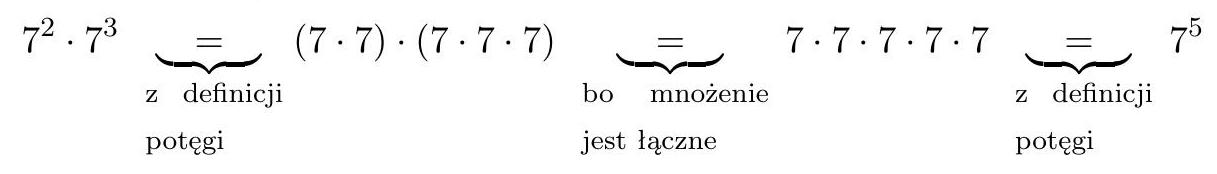
\includegraphics[max width=\textwidth]{2024_11_21_8f01584889ff06348ae7g-080}
\end{center}

Podobnie

\[
x^{3} \cdot x^{5}=(x \cdot x \cdot x) \cdot(x \cdot x \cdot x \cdot x \cdot x)=x \cdot x \cdot x \cdot x \cdot x \cdot x \cdot x \cdot x=x^{8}
\]

Ogólnie\\
\(a^{n} \cdot a^{p}=a^{n+p} \quad\) gdzie \(a-\) dowolna liczba, \(n, p-\) liczby naturalne\\
3. Zapisz w postaci jednej potęgi ( \(a, b, x\) oznaczają dowolną liczbę)\\
a) \(2^{14} \cdot 2^{15} \cdot 2^{16}=\)\\
b) \(x^{30} \cdot x^{32} \cdot x^{34}=\)\\
c) \(a^{9} \cdot a^{11} \cdot a^{10}=\)\\
d) \(3^{10} \cdot 3^{10} \cdot 3^{10}=\)\\
e) \(a^{3} \cdot a^{4} \cdot a^{2}=\)\\
f) \(a^{3} \cdot a^{2} \cdot a \cdot a^{4}=\)\\
4. W miejsce kropek wstaw odpowiedni wykładnik, aby zachodziła równość:\\
a) \(7^{4} \cdot 7^{\cdots \cdots \cdots \cdot} \cdot 7^{5}=7^{16}\)\\
b) \(5^{3} \cdot 5^{\cdots \cdots} \cdot 5^{4}=5^{15}\)\\
c) \(25 \cdot 5^{\cdots \cdots \cdots} \cdot 125=5^{10}\)\\
d) \(36 \cdot 6^{5} \cdot 6^{\cdots \cdots \cdot}=6^{12}\)\\
e) \(16 \cdot 2^{\cdots \cdots \cdots} \cdot 8=2^{13}\)\\
f) \(9 \cdot 3 \cdots \cdots \cdots \cdot 81=3^{13}\)\\
g) \(64 \cdot 16 \cdot 4^{\cdots \cdots}=4^{11}\)\\
h) \(64 \cdot 2^{\cdots \cdots \cdots} \cdot 512=2^{20}\)\\
i) \(256 \cdot 2^{\cdots \cdots \cdots \cdot} \cdot 128=2^{19}\)

\subsection*{4.2 Iloraz potęg o równej podstawie}
\section*{PRZYKŁADY}
\[
\begin{gathered}
\frac{5^{4}}{5^{2}}=\frac{5 \cdot 5 \cdot 5 \cdot 5}{5 \cdot 5}=\underbrace{\frac{5}{5} \cdot \frac{5}{5}}_{=1} \cdot 5 \cdot 5=5^{2} \\
\frac{2^{7}}{2^{4}}=\frac{2 \cdot 2 \cdot 2 \cdot 2 \cdot 2 \cdot 2 \cdot 2}{2 \cdot 2 \cdot 2 \cdot 2}=\underbrace{\frac{2}{2} \cdot \frac{2}{2} \cdot \frac{2}{2} \cdot \frac{2}{2}}_{=1} \cdot 2 \cdot 2 \cdot 2=2^{3} \\
\frac{x^{5}}{x^{2}}=\frac{x \cdot x \cdot x \cdot x \cdot x}{x \cdot x}=\underbrace{\frac{x}{x} \cdot \frac{x}{x}}_{=1} \cdot x \cdot x \cdot x=x^{3}
\end{gathered}
\]

Teraz powinieneś już zauważyć, że \(\frac{x^{6}}{x^{2}}=x^{4}, \frac{7^{15}}{7^{4}}=7^{11}\), itd.\\
Ogólnie

\[
\frac{a^{n}}{a^{p}}=a^{n-p} \quad \text { gdzie } a \neq 0, n, p-\text { liczby nat. przy czym } n>p
\]

\begin{enumerate}
  \setcounter{enumi}{4}
  \item Wykonaj dzielenie poniższych potęg zapisując wynik jako pojedynczą potęge, tak jak w poprzednich przykładach.\\
a) \(\frac{x^{7}}{x^{3}}=\)\\
b) \(\frac{11^{15}}{11^{3}}=\)\\
c) \(\frac{10^{14}}{10^{5}}=\)\\
d) \(\frac{1007^{1007}}{1007^{1000}}=\)\\
e) \(\frac{12^{231}}{12^{229}}=\)\\
f) \(\frac{34^{33}}{34^{23}}=\)\\
g) \(\frac{y^{60}}{y^{56}}=\)\\
h) \(\frac{10^{8}}{10^{5}}=\)
  \item W miejsce kropek wstaw liczby tak, aby zachodziły równości\\
a) \(5^{5} \cdot 5^{\cdots \cdots \cdots}: 5^{7}=5^{2}\)\\
b) \(9^{7} \cdot 9^{2}: 9^{\cdots \cdots \cdots}=9^{3}\)\\
c) \(2^{10} \cdot 4: 2^{\cdots \cdots \cdots}=2^{4}\)\\
d) \(7^{9} \cdot 7^{7}: 7^{\cdots \cdots \cdots}=7^{10}\)\\
e) \(6^{5} \cdot 6^{6}: 6^{\cdots \cdots \cdots}=6^{8}\)\\
f) \(3^{11} \cdot 27: 3^{\cdots \cdots \cdots}=3^{8}\)\\
g) \(125 \cdot 5^{\cdots \cdots \cdots}: 25=5^{6}\)\\
h) \(64 \cdot 256: 4^{\cdots \cdots \cdot}=4^{5}\)\\
i) \(81 \cdot 243: 3^{\cdots \cdots}=3^{3}\)
\end{enumerate}

\subsection*{4.3 Potęga iloczynu i ilorazu}
UWAGA W matematyce jest bardzo powszechnie przyjęta umowa: o ile to nie prowadzi do nieporozumienia, to znak mnożenia pomijamy.

\section*{PRZYKŁADY}
Iloczyn \(3 \cdot a\) zapisujemy krótko \(3 a\)\\
Iloczyn \(25 \cdot a \cdot b \cdot c^{2}\) zapisujemy krótko \(25 a b c^{2}\)\\
Iloczyn \(2 \cdot a \cdot b\) zapisujemy krótko \(2 a b\).\\
PRZYKŁADY potęg iloczynu\\
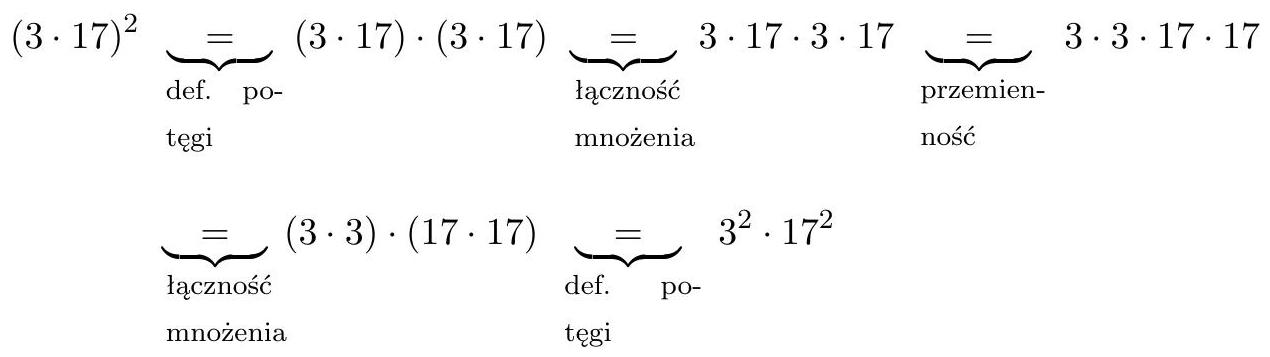
\includegraphics[max width=\textwidth, center]{2024_11_21_8f01584889ff06348ae7g-082}

Podobnie

\[
\begin{aligned}
(a \cdot b)^{3} & \underbrace{=}_{\text {def. potęgi }}(a \cdot b) \cdot(a \cdot b) \cdot(a \cdot b)=a \cdot b \cdot a \cdot b \cdot a \cdot b=a \cdot a \cdot a \cdot b \cdot b \cdot b \\
& =(a \cdot a \cdot a) \cdot(b \cdot b \cdot b) \underbrace{=}_{\text {def. potęgi }} a^{3} \cdot b^{3} \underbrace{=}_{\text {pominięty znak }} a^{3} b^{3}
\end{aligned}
\]

I podobnie, pisząc już krótko,

\[
(-2 a b)^{2}=(-2)^{2} a^{2} b^{2}=4 a^{2} b^{2}
\]

Ogólnie

\[
(a \cdot b)^{n}=a^{n} \cdot b^{n} \quad \text { gdzie } a, b-\text { dowolne liczby, } n-1 \text {.nat. }
\]

\begin{enumerate}
  \setcounter{enumi}{6}
  \item Uwzględniając powyższą umowę oraz własności potęgi podnieś do podanej potęgi poniższe iloczyny, tak jak w powyższych przykładach:\\
a) \((2 x)^{2}=\)\\
b) \((3 p q)^{3}=\)\\
c) \((2 m)^{3}=\)\\
d) \((-2 m n)^{2}=\)\\
e) \((-3 a b)^{3}=\)\\
f) \([(-3) x]^{4}=\)
\end{enumerate}

PRZYKŁADY potęgi ilorazu

\[
\left(\frac{5}{7}\right)^{3} \underbrace{=}_{\text {def. potęgi }} \frac{5}{7} \cdot \frac{5}{7} \cdot \frac{5}{7} \underbrace{=}_{\substack{\text { mnożenie } \\ \text { ułamków }}} \frac{5 \cdot 5 \cdot 5}{7 \cdot 7 \cdot 7} \underbrace{=}_{\text {def. potęgi }} \frac{5^{3}}{7^{3}}
\]

Ogólnie

\[
\left(\frac{a}{b}\right)^{n}=\frac{a^{n}}{b^{n}} \quad \begin{aligned}
& \text { gdzie } \quad a-\text { dow. liczba, } b-\text { dow. liczba różna od } 0, \\
& n \text {-dow. liczba naturalna }
\end{aligned}
\]

\begin{enumerate}
  \setcounter{enumi}{7}
  \item Wpierw zapisz w postaci jednej potęgi, a następnie oblicz:\\
a) \(\frac{44^{5}}{22^{5}}=\)\\
b) \(\frac{3^{3}}{0,3^{3}}=\)\\
c) \(\frac{65^{3}}{13^{3}}=\)\\
d) \(\frac{1024^{4}}{512^{4}}=\)\\
e) \(\frac{9^{5}}{3^{5}}=\)\\
f) \(\frac{128^{4}}{64^{4}}=\)\\
g) \(\left(\frac{3}{7}\right)^{4}:\left(\frac{1}{7}\right)^{4}=\)\\
h) \(\left(3 \frac{3}{4}\right)^{4}:\left(\frac{3}{4}\right)^{4}=\)\\
i) \((6,5)^{2}:(0,13)^{2}=\)
\end{enumerate}

\subsection*{4.4 Potęga potęgi}
\section*{PRZYKŁADY}
\[
\begin{aligned}
\left(2^{4}\right)^{2} & =\left(2^{4}\right) \cdot\left(2^{4}\right)=(2 \cdot 2 \cdot 2 \cdot 2) \cdot(2 \cdot 2 \cdot 2 \cdot 2)=2^{8} \\
\left(5^{2}\right)^{3} & =\left(5^{2}\right) \cdot\left(5^{2}\right) \cdot\left(5^{2}\right)=(5 \cdot 5) \cdot(5 \cdot 5) \cdot(5 \cdot 5)=5^{6} \\
81^{5} & =\left(3^{4}\right)^{5}=3^{20}
\end{aligned}
\]

Ogólnie

\[
\left(a^{p}\right)^{n}=a^{p \cdot n} \quad \begin{aligned}
& \text { gdzie } a-\text { dowolna liczba, } \\
& \\
& p, n-\text { dowolne liczny całkowite dodatnie }
\end{aligned}
\]

\begin{enumerate}
  \setcounter{enumi}{8}
  \item W miejsce kropek wstaw odpowiednie liczby:\\
a) \(4^{3}=2^{\cdots} \cdots\)\\
b) \(9^{4}=3 \cdots \cdots\)\\
c) \(125^{3}=5 \cdots \cdots\)\\
d) \(3^{20}=(\ldots \ldots \ldots)^{10}\)\\
e) \(5^{10}=(\ldots \ldots . .)^{5}\)\\
f) \(243^{5}=3^{\cdots} \cdots\)
  \item Ponieważ \((2 a)^{2}=4 a^{2}\), mówimy więc, że \(4 a^{2}\) jest kwadratem wyrażenia \(2 a\). Podobnie \(9 x^{2} y^{4}\) jest kwadratem wyrażenia \(3 x y^{2}\), co zapisujemy krótko \(9 x^{2} y^{4}=\left(3 x y^{2}\right)^{2}\). Zapisz w podobny sposób w postaci kwadratu następujące wyrażenia. Tutaj dla ułatwienia powiemy, że współczynniki liczbowe są kwadratami liczb naturalnych.\\
a) \(144 a^{2}=\)\\
b) \(64 y^{2}=\)\\
c) \(441 y^{2}=\)\\
d) \(81 x^{2} y^{2}=\)\\
e) \(121 b^{4}=\)\\
f) \(400 z^{4}=\)\\
g) \(169 x^{6}=\)\\
h) \(361 a^{4} b^{4}=\)\\
i) \(225 x^{2} y^{4}=\)\\
j) \(49 x^{4} y^{6}=\)\\
k) \(196 a^{4} b^{2}=\)
\end{enumerate}

\begin{enumerate}
  \item \(961 x^{6} y^{2}=\)
\end{enumerate}

\begin{enumerate}
  \setcounter{enumi}{10}
  \item Każde z poniższych wyrażeń arytmetycznych czy też algebraicznych zapisz jako kwadrat odpowiedniego wyrażenia lub też liczby:\\
a) \(0=\)\\
b) \(1=\)\\
c) \(2^{6}=\)\\
d) \(10^{8}=\)\\
e) \(4^{4}=\)\\
f) \(a^{8}=\)\\
g) \(a^{6} b^{6}=\)\\
h) \(a^{6} b^{4} c^{2}=\)\\
i) \(16 a^{4} b^{6}=\)\\
j) \(3 \cdot 3^{3}=\)\\
k) \(7 \cdot 7^{5}=\)
\end{enumerate}

\begin{enumerate}
  \item \(9 \cdot 2^{8}=\)\\
m) \(8 \cdot 18 a^{4}=\)\\
n) \(3 \cdot 15^{3} \cdot 125=\)\\
o) \(4^{3}=\)\\
p) \(9^{5}=\)\\
q) \(16^{5}=\)\\
r) \(3 \cdot 12^{3}=\)\\
s) \(5 \cdot 80^{3}=\)\\
t) \(3 \cdot 75^{3}=\)\\
u) \(2 \cdot 18^{5}=\)
\end{enumerate}

UMOWA dotycząca napisów \(a^{b^{c}} \mathrm{i}\left(a^{b}\right)^{c}\) objaśniona na przykładach

\[
4^{2^{3}}=4^{\left(2^{3}\right)}=4^{8} \quad \text { natomiast } \quad\left(4^{2}\right)^{3}=4^{2} \cdot 4^{2} \cdot 4^{2}=4^{2+2+2}=4^{6}
\]

\begin{enumerate}
  \setcounter{enumi}{11}
  \item W miejsce kropek wstaw jeden ze znaków \(<,=,>\), tak aby otrzymać zdanie prawdziwe:\\
a) \(\left(7^{3}\right)^{4}\) \(\left(7^{4}\right)^{3}\)\\
b) \(16^{8}\)\\
\(.64^{5}\)\\
c) \((0,5)^{7} \ldots \ldots \ldots(0,25)^{4}\)\\
d) \(\left(5^{4}\right)^{2}\) \(.5^{4^{2}}\)\\
e) \(27^{15}\)\\
\(.9^{17}\)\\
f) \(2^{2^{2}}\)\\
g) \(3^{3^{3}}\) ........ \(\left(3^{3}\right)^{3}\)
  \item Wykonaj następujące działania:\\
a) \(\left(a^{4} \cdot a^{3}\right): a^{2}=\)\\
b) \(m^{9}:\left[\left(m^{3}: m\right) \cdot m^{5}\right]=\)\\
c) \(\left(x^{7}: x^{3}\right): x^{4}=\)\\
d) \(\left[\left(z^{4}\right)^{2} \cdot z^{3}: z^{7}\right]^{2}=\)\\
e) \(\left[b \cdot\left(b^{2} \cdot b^{4}\right)\right]^{3}: b^{5}=\)\\
f) \(\left[x^{14}: x^{9}\right]^{2}: x=\)\\
g) \(\left(x^{2} \cdot x^{4}\right):\left(x^{3} \cdot x\right)=\)\\
h) \(\left(y^{5}: y\right)^{3}:\left(y^{7}: y^{2}\right)=\)\\
i) \(\left(\frac{a^{2} b^{3}}{c^{4}}\right)^{3}=\)\\
j) \(\left(\frac{3 a^{2}}{b^{3}}\right)^{4}=\)\\
k) \(\left(\frac{3 b^{2}}{2 c^{3}}\right)^{3}=\)
  \item Korzystając z odpowiednich wzorów zapisz poniższe wyrażenia w postaci jednej liczby.\\
a) \(\left(3: 10^{2}\right)^{3}=\)\\
b) \(2^{3}: 10^{5}=\)\\
c) \(3^{3}: 10^{4}=\)\\
d) \(\left(3 \cdot 10^{2}\right)^{3}=\)\\
e) \(200^{4}=\)\\
f) \(\left(5 \cdot 10^{2}\right)^{3}=\)
  \item Wyznacz połowę połowy liczby \(16^{20}\) i zapisz ją w postaci potęgi o podstawie 4.
  \item Populacja bakterii podwaja się po upływie każdej godziny. Ile razy zwiększyła się liczba bakterii po upływie 10 godzin w stosunku do stanu wyjściowego, przy założeniu, że w tym czasie bakterie nie umierały.
\end{enumerate}

\subsection*{4.5 Jednomiany}
Jednomiany są to wyrażenia będące iloczynami liczb oraz zmiennych. Szczególnym przypadkiem jednomianu jest liczba czy też pojedyncza zmienna. Zmienne są to miejsca, w które możemy wstawiać liczby.

\section*{PRZYKŁADY}
\(2 a b, 3 x y^{2} z, \frac{1}{2} a b^{2} c^{4}, 12 x^{3} y z^{3}, a,-12 a b^{2}\).\\
PRZYKŁADY wyrażeń nie będących jednomianami:\\
\(a+b, 3 x+y, 4 a^{2}+1,(a-3 b)^{2}\).

Jeżeli w jednomianie zmienne zastąpimy liczbami, to otrzymujemy wyrażenie arytmetyczne będace iloczynem liczb.

\section*{PRZYKŁADY}
\begin{center}
\begin{tabular}{c|c|c|c}
jednomian & podstawienie & wyrażenie arytm. & wartość wyrażenia \\
\hline
\(3 a b\) & \(a=2, b=5\) & \(3 \cdot 2 \cdot 5\) & 30 \\
\(-a^{2}\) & \(a=3\) & \(-3^{2}\) & -9 \\
\(x^{2}\) & \(x=-3\) & \((-3)^{2}\) & 9 \\
\(3 a^{2} b c^{5}\) & \(a=2, b=-3, c=1\) & \(3 \cdot 2^{2} \cdot(-3) \cdot 1^{5}\) & -36 \\
\(-2 a^{2} b^{2}\) & \(a=3, b=2\) & \(-2 \cdot 3^{2} \cdot 2^{2}\) & -72 \\
\end{tabular}
\end{center}

\section*{UMOWA}
Wpierw zapisujemy współczynnik liczbowy, a następnie w porządku alfabetycznym współczynniki literowe. Jeżeli kilka czynników jest takich samych, to zapisujemy ich iloczyn w postaci potęgi. Znaki mnożenia pomijamy. Dodatkowo, jeżeli współczynnik liczbowy jest równy 1, to go pomijamy, a gdy jest równy -1 , to zamiast niego piszemy znak - czyli zamiast pisać \(1 x\) piszemy \(x\), zaś zamiast pisać \(-1 y\) czy też \((-1) \cdot y\) piszemy \(-y\)

\section*{PRZYKŁADY}
\begin{center}
\begin{tabular}{ll}
Iloczyn & Zapisany zgodnie z konwencją \\
\(4 \cdot a \cdot b \cdot a\) & \(4 a^{2} b\) \\
\(a \cdot(-3) \cdot x \cdot b^{2}\) & \(-3 a b^{2} x\) \\
\(d \cdot(-2) \cdot b \cdot b \cdot t\) & \(-2 b^{2} d t\) \\
\(1 x y^{2} z\) & \(x y^{2} z\) \\
\(-1 x^{2} y\) & \(-x^{2} y\) \\
\end{tabular}
\end{center}

PRZYKŁADY jednomianów zapisanych niezgodnie z konwencją: \(4 z x, 15 x^{2} t, a 15 b\).\\
17. Oblicz wartość poniższych jednomianów dla podanych wartości liczbowych\\
a) \(a^{2} b^{3} \quad\) dla \(\quad a=2, b=-3\),\\
b) \(4 a^{3} b \quad\) dla \(a=2, b=\frac{1}{4}\),\\
c) \(5 a b^{3} c^{2} \quad\) dla \(\quad a=2, b=1, c=3\)\\
d) \(2 a b c^{4} \quad\) dla \(\quad a=3, b=2, c=\frac{1}{2}\)\\
e) \(\quad-3 a^{2} b^{2} c \quad\) dla \(\quad a=-2, b=3, c=2\),\\
f) \(\quad-b^{4} c d^{2} \quad\) dla \(\quad b=-1, c=7, d=3\),\\
g) \(-7 a b^{2} c^{3} \quad\) dla \(\quad a=-2, b=2, c=-1\),\\
h) \(x^{2} y^{3} \quad\) dla \(\quad x=-3, y=-2\)\\
i) \(-3 a b^{2} \quad\) dla \(\quad a=-1, b=-3\),\\
j) \(\quad(-2 a b)^{2} \quad\) dla \(\quad a=2, b=1\),\\
k) \(-2(a b)^{2} \quad\) dla \(\quad a=2, b=-1\),\\
l) \(-2(-a b)^{2} \quad\) dla \(\quad a=2, b=3\),\\
m) \(-3 a^{2} b \quad\) dla \(a=-2, b=3\),

\subsection*{4.6 Mnożenie jednomianów}
\section*{FAKT}
Iloczyn dwóch jednomianów jest jednomianem czyli również potęga jednomianu jest jednomianem. Mnożąc przez siebie jednomiany korzystamy z przemienności i łączności mnożenia, a wynik zapisujemy zgodnie z konwencją o zapisie jednomianów.

\section*{PRZYKŁADY wyjaśniające}
\[
\begin{aligned}
& 12 x y^{2} \cdot 3 x^{2} z=3 \cdot 12 \cdot x \cdot x^{2} \cdot y^{2} \cdot z=36 x^{3} y^{2} z \\
& 4 x \cdot 5 y=4 \cdot 5 \cdot x \cdot y=20 x y \\
& 4 x \cdot(-3) y=-3 \cdot 4 \cdot x \cdot y=-12 x y \\
& -2 x^{2} y \cdot 4 a y^{2}=(-2) \cdot 4 \cdot x^{2} \cdot y \cdot a \cdot y^{2}=-8 a x^{2} y^{3} \\
& -7 a b \cdot\left(-2 a^{3} b x^{2}\right)=(-2) \cdot(-7) \cdot a \cdot b \cdot a^{3} \cdot b \cdot x^{2}=14 a^{4} b^{2} x^{2} \\
& (3 x)^{2}=3^{2} x^{2}=9 x^{2} \\
& \left(2 a b^{2}\right)^{3}=2 a b^{2} \cdot 2 a b^{2} \cdot 2 a b^{2}=2 \cdot 2 \cdot 2 \cdot a \cdot a \cdot a \cdot b^{2} \cdot b^{2} \cdot b^{2}=2^{3} a^{3}\left(b^{2}\right)^{3}=8 a^{3} b^{6}
\end{aligned}
\]

\begin{enumerate}
  \setcounter{enumi}{17}
  \item Korzystając z powyższych przykładów zapisz wynik poniższych działań w postaci jednomianu. Staraj się zapisać od razu finalną odpowiedź.\\
a) \(4 a b^{2} \cdot 7 a^{2} b^{3}=\)\\
b) \(x^{2} y \cdot 5 w^{2} y^{2} \cdot z=\)\\
c) \(4 x^{2} y \cdot 5 x y^{3}=\)\\
d) \(2 x^{5} y^{2} \cdot x y^{3}=\)\\
e) \(4 x^{3} y^{2} \cdot(-2 x y)=\)\\
f) \(-3 a^{2} b^{2} c \cdot(-5) a b^{4}=\)\\
g) \(2 x^{4} y^{3} \cdot\left(-x^{2} y\right) \cdot\left(-3 x^{3} y^{2} z\right)=\)\\
h) \(-7 a b \cdot\left(-4 a^{2} b\right)=\)\\
i) \(-3 x y \cdot 2 x^{2} y^{3} \cdot\left(-3 x y^{2}\right)=\)\\
j) \(4 x^{2} \cdot 5 x y \cdot 2 x^{3} y=\)\\
k) \(-5 x y^{2} \cdot 4 x^{2} y^{3} \cdot(-2 x y z)=\)\\
l) \(-2 a c^{2} \cdot 3 a b^{2} c^{2}=\)
  \item Wykonaj, podobnie jak powyżej, następujące działania.\\
a) \(x^{2} \cdot x^{4}=\)\\
b) \(\left(a b^{2}\right) \cdot\left(a^{5} b^{4}\right)=\)\\
c) \(\left(16 x^{5} y\right) \cdot\left(4 x^{2} y^{14}\right)=\)\\
d) \(\left(4 x^{7} y\right) \cdot\left(2 x^{2} y^{2}\right)=\)\\
e) \(\left(p q^{2}\right)^{2} \cdot\left(p q^{2} r^{12}\right)=\)\\
f) \(\left(3 y^{2}\right)^{3} \cdot\left(3 y^{2}\right) \cdot y^{5}=\)\\
g) \(5 t^{5} \cdot\left(25 t^{4} y^{21}\right)=\)\\
h) \(\left(12 x^{4} y^{5}\right) \cdot\left(13 x^{11} y^{4}\right)=\)
  \item Wykonaj następujące działania. Wynik zapisz w postaci jednomianu.\\
a) \((-2 x)^{2} \cdot(-2 x)^{2}=\)\\
b) \((2 x)^{2} \cdot(-2 x)^{3}=\)\\
c) \((-2 x)^{2} \cdot(-2 y)^{2}=\)\\
d) \((-2 x)^{2} \cdot(3 y)^{2}=\)\\
e) \((-2 x)^{2} \cdot(-3 y)^{2}=\)\\
f) \((-2 x)^{3} \cdot(-3 y)^{2}=\)
  \item Wykonaj następujące działania. Wynik zapisz w postaci jednomianu.\\
a) \(a^{2} b \cdot a b=\)\\
b) \(a^{2} b^{3} \cdot a^{4} b^{2}=\)\\
c) \(a^{2} \cdot a \cdot b^{3} \cdot b^{5} \cdot b^{2}=\)\\
d) \(x^{4} \cdot x^{9} \cdot y^{2} \cdot x \cdot y^{4} \cdot x^{2}=\)\\
e) \(a^{3} \cdot b^{2} \cdot c \cdot a \cdot b^{3} \cdot a \cdot b^{4} \cdot c^{3}=\)
\end{enumerate}

\subsection*{4.7 Dzielenie jednomianów}
\section*{PRZYKŁADY}
\[
\begin{aligned}
& \frac{4 a^{2} b^{3}}{2 a b}=\frac{4 \cdot a^{2} \cdot b^{3}}{2 \cdot a \cdot b}=\frac{4}{2} \cdot \frac{a^{2}}{a} \cdot \frac{b^{3}}{b}=2 \cdot a \cdot b^{2}=2 a b^{2} \\
& \frac{44 a^{2} b^{5} c}{11 a^{2} b^{4}}=\frac{44}{11} \cdot \frac{a^{2}}{a^{2}} \cdot \frac{b^{5}}{b^{4}} \cdot c=4 \cdot 1 \cdot b \cdot c=4 b c
\end{aligned}
\]

\begin{enumerate}
  \setcounter{enumi}{21}
  \item Zapisz wynik poniższych działań w postaci jednomianu:\\
a) \(\frac{12 x^{4} y^{3}}{4 x y^{2}}=\)\\
b) \(\frac{15 x^{3} y^{3}}{3 x^{2} y}=\)\\
c) \(\frac{7^{12} a^{4} b^{3}}{7^{10} a b^{2}}=\)\\
d) \(\frac{12 x^{4} y^{2} z}{3 x^{2} y^{2}}=\)\\
e) \(\frac{-15 x^{2} y}{3 x y}=\)\\
f) \(\frac{-6 x^{4} y^{2}}{-2 x^{2} y}=\)\\
g) \(\frac{-4 x^{4} y^{5}}{2 x^{2} y^{4}}=\)\\
h) \(\frac{8 x^{2} y^{2}}{-4 x y^{2}}=\)\\
i) \(\frac{24 x^{4} y^{2} z}{-3 x y^{2} z}=\)\\
j) \(\frac{9 x y}{-9 x y}=\)\\
k) \(\frac{-7 x^{2} y^{3}}{-7 x^{2} y^{3}}=\)
\end{enumerate}

\begin{enumerate}
  \item \(\frac{-33 a b^{2} c^{3}}{11 a b^{2} c^{3}}=\)
\end{enumerate}

\section*{Odpowiedzi.}
\begin{enumerate}
  \item a) \(-\frac{1}{10}\) b) 0 c) -96 d) -4 e) -10 f) -4 g) 9 h) -123 i) 31 j) 39
  \item a) 27 b) 13 c) 32 d) 25 e) 49 f) \(2 \frac{1}{4}\) g) \(-\frac{7}{9}\) h) \(-5 \frac{1}{3}\) i) \(-9 \frac{1}{8}\) j) \(\frac{1}{72}\) k) \(6 \frac{3}{4}\) l) \(\left.\left.-10 \mathrm{~m}\right)-3 \frac{3}{8} \mathrm{n}\right) 8 \frac{3}{4}\)
  \item a) \(2^{45}\) b) \(x^{96}\) c) \(a^{30}\) d) \(3^{30}\) e) \(a^{9}\) f) \(a^{10}\)
  \item a) 7 b) 8 c) 5 d) 5 e) 6 f) 7 g) 6 h) 5 i) 4
  \item a) \(x^{4}\) b) \(11^{12}\) c) \(10^{9}\) d) \(1007^{7}\) e) \(12^{2}\) f) \(34^{10}\) g) \(y^{4}\) h) \(10^{3}\)
  \item a) 4 b) 6 c) 8 d) 6 e) 3 f) 6 g) 5 h) 2 i) 6
  \item a) \(4 x^{2}\) b) \(27 p^{3} q^{3}\) c) \(8 m^{3}\) d) \(4 m^{2} n^{2}\) e) \(-27 a^{3} b^{3}\) f) \(81 x^{4}\)
  \item a) 32\\
b) 1000\\
c) 125\\
d) 16 e) 243\\
f) 16 g\() 81\)\\
h) 625\\
i) 2500
  \item a) 6 b) 8 c) 9 d) 9 e) 25 f) 25
  \item a) \((12 a)^{2}\) b) \((8 y)^{2}\) c) \((21 y)^{2}\) d) \((9 x y)^{2}\) e) \(\left(11 b^{2}\right)^{2}\) f) \(\left(20 z^{2}\right)^{2}\) g) \(\left(13 x^{3}\right)^{2}\) h) \(\left(19 a^{2} b^{2}\right)^{2}\) i) \(\left(15 x y^{2}\right)^{2}\) j) \(\left(7 x^{2} y^{3}\right)^{2}\) k) \(\left(14 a^{2} b\right)^{2}\) l) \(\left(31 x^{3} y\right)^{2}\)
  \item a) \(0^{2}\) b) \(1^{2}\) c) \(\left(2^{3}\right)^{2}\) d) \(\left(10^{4}\right)^{2}\) e) \(\left(4^{2}\right)^{2}\) f) \(\left(a^{4}\right)^{2}\) g) \(\left(a^{3} b^{3}\right)^{2}\) h) \(\left(a^{3} b^{2} c\right)^{2}\) i) \(\left(4 a^{2} b^{3}\right)^{2}\) j) \(\left.\left(3^{2}\right)^{2} \mathrm{k}\right)\left(7^{3}\right)^{2}\) l) \(\left.\left.\left(3 \cdot 2^{4}\right)^{2} \mathrm{~m}\right)\left(12 a^{2}\right)^{2} \mathrm{n}\right)\left(3^{2} \cdot 5^{3}\right)^{2}\) o) \(\left(2^{3}\right)^{2}\)\\
p) \(\left(3^{5}\right)^{2}\) q) \(\left(4^{5}\right)^{2}\) r) \(\left(8 \cdot 3^{2}\right)^{2}\) s) \(\left(5^{2} \cdot 2^{6}\right)^{2}\) t) \(\left(3^{2} \cdot 5^{3}\right)^{2}\) u) \(\left(2^{3} \cdot 5^{5}\right)^{2}\)
  \item a) \(=\), b) \(>\), c) \(>\), d) \(<\), e) \(>\), f) \(=\), g) \(>\)
  \item a) \(a^{5}\) b) \(m^{2}\) c) 1 d) \(z^{8}\) e) \(b^{16}\) f) \(x^{9}\) g) \(x^{2}\) h) \(y^{7}\) i) \(\frac{a^{6} b^{9}}{c^{12}}\) j) \(\frac{81 a^{8}}{b^{12}}\) k) \(\frac{27 b^{6}}{8 c^{9}}\)
  \item a) 0,000027 b) 0,00008 c) 0,0027 d) \(27,000,000\) e) \(1,600,000,000\) f) \(125,000,000\)
  \item \(4^{39}\)
  \item 1024 razy
  \item a) -108 b) 8 c) 90 d) \(\frac{3}{4}\) e) -216 f) -63 g) -56 h) -72 i) 27 j) 16 k) -8 l) \(-72 \mathrm{~m})-36\)
  \item a) \(28 a^{3} b^{5}\), b) \(5 w^{2} x^{2} y^{3} z\), c) \(20 x^{3} y^{4}\), d) \(2 x^{6} y^{5}\), e) \(-8 x^{4} y^{3}\), f) \(15 a^{3} b^{6} c\), g) \(6 x^{9} y^{6} z\), h) \(28 a^{3} b^{2}\), i) \(18 x^{4} y^{6}\), j) \(40 x^{6} y^{2}\), k) \(40 x^{4} y^{6} z\), l) \(-6 a^{2} b^{2} c^{4}\)
  \item a) \(x^{6}\) b) \(a^{6} b^{6}\) c) \(64 x^{7} y^{15}\) d) \(8 x^{9} y^{3}\) e) \(p^{3} q^{6} r^{12}\) f) \(81 y^{13}\) g) \(125 t^{9} y^{21}\) h) \(156 x^{15} y^{9}\)
  \item a) \(16 x^{4}\) b) \(-32 x^{5}\) c) \(16 x^{2} y^{2}\) d) \(36 x^{2} y^{2}\) e) \(36 x^{2} y^{2}\) f) \(-72 x^{3} y^{2}\)
  \item a) \(a^{3} b^{2}\) b) \(a^{6} b^{5}\) c) \(a^{3} b^{10}\) d) \(x^{16} y^{6}\) e) \(a^{5} b^{9} c^{4}\)
  \item a) \(3 x^{3} y\) b) \(5 x y^{2}\) c) \(49 a^{3} b\) d) \(4 x^{2} z\) e) \(-5 x\) f) \(3 x^{2} y\) g) \(-2 x^{2} y\) h) \(-2 x\) i) \(-8 x^{3}\) j) -1 k) 1 l) -3
\end{enumerate}

\section*{Rozdział 5}
\section*{WYRAŻENIA ALGEBRAICZNE}
Rozpoczniemy od tworzenia wyrażeń i zapisywania wyrażeń w języku polskim. Służyć to będzie pewnemu wyrobieniu w posługiwaniu się językiem matematyki. Następnie zaczniemy zajmować się przekształcaniem wyrażeń algebraicznych.

\subsection*{5.1 Tworzenie wyrażeń algebraicznych}
\begin{enumerate}
  \item Zapisz w postaci wyrażenia:\\
a) sumę liczb \(a\) i \(b\),\\
b) sumę kwadratów liczb \(a\) i \(b\),\\
c) sumę sześcianów liczb \(a\) i \(b\),\\
d) różnicę sześcianów liczb \(a\) i \(b\),\\
e) odwrotność różnicy liczb \(a\) i \(b\),\\
f) odwrotność sumy sześcianów liczb \(a\) i \(b\),\\
g) odwrotność sumy kwadratów liczb \(a\) i \(b\),\\
h) suma odwrotności liczb \(a\) i \(b\),\\
i) suma odwrotności kwadratów liczb \(a\) i \(b\),\\
j) różnica odwrotności sześcianów liczb \(a\) i \(b\),\\
k) kwadrat różnicy liczb \(a\) i \(b\),
\end{enumerate}

\begin{enumerate}
  \item sześcian różnicy liczb \(x\) i \(y\),\\
m) kwadrat sumy kwadratów liczb \(a\) i \(b\),\\
n) kwadrat odwrotności sumy liczb \(a\) i \(b\),\\
o) kwadrat sumy odwrotności liczb \(a\) i \(b\),\\
p) kwadrat odwrotności różnicy kwadratów liczb \(a\) i \(b\),\\
q) odwrotność sumy odwrotności liczb \(a\) i \(b\),\\
r) sześcian różnicy kwadratów liczb \(a\) i \(b\).
\end{enumerate}

\begin{enumerate}
  \setcounter{enumi}{1}
  \item Zapisz w postaci wyrażenia:\\
a) kwadrat sześcianu liczby 10 ,\\
b) iloczyn sumy sześcianów liczb \(a\) i \(b\) przez kwadrat sumy kwadratów liczb \(m\) i \(n\),\\
c) suma sześcianów odwrotności liczb \(m\) i \(n\),\\
d) iloraz sumy kwadratów liczb \(a\) i \(b\) przez kwadrat różnicy \(a\) i \(b\),\\
e) kwadrat sumy liczb \(2^{100}\) i \(2^{50}\),\\
f) suma liczby \(a\) i kwadratu liczby \(b\),\\
g) różnica sześcianu liczby \(b\) i liczby 4 ,\\
h) iloraz kwadratu liczby a przez 5,\\
i) iloczyn liczby -2 , kwadratu liczby \(a\) i sześcianu liczby \(b\),\\
j) podwojony iloczyn liczby \(a\) i kwadratu sumy liczb \(x\) i \(y\),\\
k) iloraz różnicy kwadratów liczb \(a\) i \(b\) przez sześcian liczby \(c\).
  \item Zapisz w języku polskim następujące wyrażenia algebraiczne:\\
a) \(a+b+c\)\\
b) \(\frac{1}{x+y}\)\\
c) \(\frac{1}{x+y^{2}}\)\\
d) \(\frac{1}{x^{2}}+\frac{1}{y^{3}}\)\\
e) \(\frac{1}{a^{3}+b^{2}}\)\\
f) \(\frac{1}{a-x^{3}}\)\\
g) \(\frac{1}{(a+b)^{2}}\)\\
h) \(\frac{1}{\left(a^{3}-b^{2}\right)^{2}}\)\\
i) \(\frac{1}{a^{3}}-\frac{1}{b^{2}}\)\\
j) \(a^{3}+b^{2}\)\\
k) \(x^{3}-y^{3}\)\\
l) \((x+y+z)^{3}\)\\
m) \((a+b)\left(x^{2}-y^{2}\right)\)\\
n) \((a-b)\left(x^{3}+y^{3}\right)\)\\
o) \(\left(a^{2}-b^{2}\right)\left(a^{2}+b^{2}\right)\)
  \item Oznaczając przez \(n\) dowolną liczbę naturalną, zapisz:\\
a) liczbę o 2 od niej mniejszą,\\
b) liczbę o 3 od niej większą,\\
c) liczbę trzy razy od niej większą,\\
d) trzy kolejne liczby naturalne,\\
e) liczbę o 1 większą od kwadratu liczby \(n\),\\
f) sześcian liczby o 1 większej od liczby \(n\).
  \item Niech \(k\) oznacza liczbę całkowitą. Zauważ, że wówczas niezależnie od tego czy \(k\) jest liczbą parzystą, czy też nieparzystą, liczba \(2 k\) jest liczbą parzystą, zaś liczba \(2 k+1\) jest liczbą nieparzystą. Zapisz trzy kolejne liczby:\\
a) nieparzyste, następujące bezpośrednio po liczbie \(2 k\),\\
b) parzyste, następujące bezpośrednio po liczbie \(2 k\),\\
c) parzyste, bezpośrednio poprzedzające liczbę \(2 k+1\).
\end{enumerate}

\section*{LICZBA, ZAPIS LICZBY.}
Liczba jest pojęciem abstrakcyjnym, natomiast zapis liczby nie jest takim pojęciem. Na co dzień nie czynimy rozróżnienia pomiędzy liczbą a zapisem liczby. Pisząc liczbę dwucyfrową o 2 dziesiątkach i 7 jednościach tworzymy napis 27 , który jako wyrażenie arytmetyczne należy rozumieć

\[
2 \cdot 10+7
\]

Zatem liczbie dwucyfrowej o \(x\) dziesiątkach i \(y\) jednościach odpowiada wyrażenie algebraiczne:

\[
x \cdot 10+y \quad \text { czyli krótko } \quad 10 x+y
\]

Podobnie liczbie trzycyfrowej o \(x\) setkach, \(y\) dziesiątek i \(z\) jedności odpowiada wyrażenie

\[
100 x+10 y+z
\]

\begin{enumerate}
  \setcounter{enumi}{5}
  \item Zapisz w postaci odpowiednich wyrażeń algebraicznych liczby:\\
(a) dwucyfrową, w której cyfra dziesiątek jest o 7 mniejsza od cyfry jedności,\\
(b) trzycyfrową, w której cyfra setek i jedności są równe, zaś cyfra dziesiątek jest równa 4,\\
(c) trzycyfrową, w której cyfra dziesiątek jest dwa razy większa od cyfry jedności, a cyfra setek jest o 2 większa od cyfry dziesiątek,\\
(d) trzycyfrową, w której cyfry jedności, dziesiątek i setek są trzema kolejnymi cyframi,\\
(e) dwucyfrową, w której cyfra dziesiątek jest dwa razy większa od cyfry jedności,\\
(f) trzycyfrową, w której cyfra jedności jest o 3 mniejsza od cyfry dziesiątek, a cyfra setek 3 razy większa od cyfry jedności.
  \item Adam ma \(x\) lat, Bartek jest 2 razy starszy od Adama, a Czesiek jest o 2 lata starszy od Adama. Zapisz w postaci odpowiednich wyrażeń\\
a) Ilość lat Bartka oraz ilość lat Cześka.\\
b) Liczbę lat Bartka 4 lata temu.\\
c) Liczbę lat Cześka za 5 lat.\\
d) Liczbę lat Bartka za 2 lata.
  \item Paweł jest cztery razy młodszy od dziadka. Niech \(x\) oznacza wiek dziadka. Zapisz w postaci wyrażenia algebraicznego wiek Pawła, gdy był on (Paweł) dwa razy młodszy niż obecnie.
  \item W wiadrze jest \(x\) litrów wody, a w beczce \(y\) litrów wody. Zapisz w postaci wyrażenia algebraicznego ilość litrów wody w wiadrze i w beczce, jeśli\\
a) z wiadra do beczki przelejemy pół litra wody,\\
b) najpierw przelejemy połowę zawartości wiadra do beczki, a potem 2 litry z beczki do wiadra,\\
c) do wiadra dolejemy \(\frac{3}{4}\) litra wody z kranu, a potem trzecią część zawartości wiadra przelejemy do beczki,\\
d) najpierw przelejemy połowę zawartości wiadra do beczki, a następnie połowę zawartości beczki do wiadra.
\end{enumerate}

\subsection*{5.2 Dodawanie (redukcja) jednomianów}
Dodawać do siebie można tylko wielkości tego samego rodzaju.

\section*{PRZYKŁADY}
Gdy do dwóch zeszytów dodamy trzy zeszyty, to mamy 5 zeszytów. Co nieco bardziej formalnie można zapisać: \(2 z+3 z=5 z\).\\
Gdy do 3 jabłek i 5 gruszek dodamy 2 jabłka i 9 gruszek, to w sumie mamy 5 jabłek i 14 gruszek. To nieco bardziej formalnie można zapisać: \(3 j+5 g+2 j+9 g=5 j+14 g\).\\
Jeszcze jeden nieco bardziej abstrakcyjny przykład: gdy do 3 metrów sznurka i 5 metrów kwadratowych materiału dodamy 4 metry sznurka i 8 metrów kwadratowych materiału, to w sumie dostaniemy 7 metrów sznurka i 13 metrów kwadratowych materiału. Ten ostatni przykład w bardziej formalny sposób możemy zapisać następująco \(3 m+5 m^{2}+4 m+8 m^{2}=7 m+13 m^{2}\).

\section*{Ogólnie}
Dodawać do siebie można tylko takie jednomiany które mają identyczne współczynniki literowe. Często zamiast zwrotu dodawanie (odejmowanie) jednomianów używamy zwrotu redukcja jednomianów.\\
Jednomiany, które mają jednakowe współczynniki literowe, a przy tym w tych samych potęgach, nazywamy jednomianami podobnymi. Różnią się one tylko współczynnikami liczbowymi.\\
Czyli dodawać do siebie możemy tylko jednomiany podobne.\\
Zasadę powyższą ilustrują poniższe

\section*{PRZYKŁADY}
\[
\begin{aligned}
& 2 x+3 y+\frac{1}{2} x+4-2 y+9+5 x=2 x+\frac{1}{2} x+5 x+3 y-2 y+4+9=7 \frac{1}{2} x+y+13 \\
& 2 x y^{2}-5 x y^{2}+4 x^{2} y+10 x y^{2}-3 x y^{2}+2 x^{2} y=4 x y^{2}+6 x^{2} y \\
& 3 x^{2}-x+5 x^{3}+6 x+11 x^{2}-2 x^{3}+x^{4}=5 x+14 x^{2}+3 x^{3}+x^{4} \\
& 2 x+3 x^{2}+11 x-3 x+2 \frac{1}{2} x^{2}-7 x y+4 x+3 x y=14 x+5 \frac{1}{2} x^{2}-4 x y
\end{aligned}
\]

\begin{enumerate}
  \setcounter{enumi}{9}
  \item Wykonaj dodawanie (redukcję) jednomianów\\
a) \(2 a+4 a-a=\)\\
b) \(2 b^{2}+12 b^{2}-3 b^{2}-b^{2}=\)\\
c) \(-3 x^{2} z+2 x^{2} z-4 x^{2} z=\)\\
d) \(-3 \frac{1}{2} x+\frac{1}{3} x-4 x=\)\\
e) \(2 a-4 b-3 b+7 a=\)\\
f) \(2 b^{2}+12 a-3 b^{2}-3 a=\)\\
g) \(13 a-5 a+2 \frac{1}{3} a-4 a+\frac{1}{2} a=\)\\
h) \(2 x y-3 x y+2 \frac{1}{5} x y+4 \frac{3}{5} x y+6 \frac{1}{5} x y=\)\\
i) \(-3 x^{2} z+2 x z-4 x^{2} z-3 x z=\)\\
j) \(4 x y+x+y-3 x y+2 x=\)\\
k) \(5 a b-10 b+8 a b-3 a+4 b-2 \frac{1}{2} a b=\)\\
l) \(40 x-26 x y+7 x-32 x y=\)\\
m) \(2 x^{2} y+3 x^{3} z-3 x y^{2}+4 x^{2} y-x^{3} z+x^{2} y=\)\\
n) \(5 a b-4 a^{2} b^{2}-8 a b^{2}+3 a b-a b^{2}-4 a^{2} b^{2}=\)
  \item Wykonaj działania:\\
a) \(x-\frac{27}{100} x-\frac{23}{100} x=\)\\
b) \(\frac{15}{100} x-\frac{2}{100} x-\frac{8}{100} x=\)\\
c) \(\frac{17}{100} x+\frac{8}{100} x-\frac{5}{100} x=\)\\
d) \(\frac{3}{100} x+\frac{27}{100} x+\frac{20}{100} x=\)\\
e) \(2 x-\frac{15}{100} x-\frac{45}{100} x-\frac{40}{100} x=\)\\
f) \(\frac{11}{100} x+\frac{13}{100} x+\frac{17}{100} x+\frac{19}{100} x=\)
\end{enumerate}

\subsection*{5.3 Dodawanie i odejmowanie sum alg.}
Zacznijmy od przykładu wprowadzającego w tę problematykę. Wyobraźmy sobie taką sytuację: ze stołu na którym leżało 12 jabłek i 8 gruszek Jacek dołożył (zabrał) 3 jabłka i 2 gruszki. W efekcie na stole w przypadku gdy dołożył jabłka i gruszki, będzie w sumie 15 jabłek i 10 gruszek, a w przypadku gdy zabrał, pozostanie 9 jabłek i 6 gruszek. Możemy to bardziej formalnie zapisać następująco:\\
w przypadku gdy dołożył

\[
(12 j+8 g)+(3 j+2 g)=15 j+10 g
\]

w przypadku, gdy zabrał

\[
(12 j+8 g)-(3 j+2 g)=9 j+6 g
\]

Obecnie będziemy mieli do czynienia z tzw. sumami algebraicznymi tzn. z takimi wyrażeniami algebraicznymi, w których po podstawieniu za zmienne liczb i wyliczeniu wartości tak uzyskanych wyrażeń arytmetycznych ostatnimi wykonywanymi działaniami będą dodawania i odejmowania. Można też powiedzieć inaczej, że suma algebraiczna jest to suma jednomianów. Jednomiany, które dodajemy (odejmujemy) nazywamy składnikami sumy.

\section*{WYJAŚNIENIE}
\(2 a+7 x y-8 a b^{2}+5\) jest to suma algebraiczna, natomiast \(2 a, 7 x y,-8 a b^{2}, 5\) sa składnikami tej sumy.

W następnych przykładach pokażemy jak uprościć wyrażenie zawierające sumę algebraiczną ujętą w nawiasy i poprzedzoną znakiem minus. W tym celu przypomnijmy fakty. które poznaliśmy w rozdziale 1 :

\[
\begin{array}{ll}
\text { F. } 1 & -a=(-1) \cdot a \\
\text { F. } 2 & -(-a)=a \\
\text { F. } 3 & a-b=a+(-b)=a+(-1) \cdot b
\end{array}
\]

oraz prawo rozdzielności mnożenia względem dodawania \(a(b+c)=a \cdot b+a \cdot c\).

\section*{WYJAŚNIENIE}
\begin{enumerate}
  \item \(-(x-4)=(-1) \cdot(x+(-4))=-1 \cdot x+(-1) \cdot(-4)=-x+4\)
  \item \(-(-3+x-2 b)=(-1) \cdot((-3)+x+(-2 b))=(-1) \cdot(-3)+(-1) \cdot x+\) \((-1) \cdot(-2 b)=3-x+2 b\)
  \item \((5 x+3 y+1)+(2 x-y)=5 x+3 y+1+2 x-y=7 x+2 y+1\)
\end{enumerate}

\section*{PRZYKŁAD wyjaśniający}
\[
\begin{aligned}
(4 x+5 y-3)-(2 x-7 y-2) & =(4 x+5 y-3)+(-1) \cdot(2 x+(-7 y)+(-2)) \\
& =4 x+5 y-3+(-1) 2 x+(-1)(-7 y)+(-1)(-2) \\
& =4 x+5 y-3-2 x+7 y+2 \\
& =2 x+12 y-1
\end{aligned}
\]

Można zatem powiedzieć, że technicznie rzecz biorąc, opuszczanie nawiasów w sumie algebraicznej sprowadza się do dwóch sytuacji:

\begin{enumerate}
  \item Jeżeli składnik sumy algebraicznej występuje w nawiasie, który to nawias poprzedzony jest znakiem plus, to nawias ten możemy opuścić nic poza tym nie zmieniając. Podobnie postępujemy, gdy przed nawiasem nie ma żadnego znaku.
  \item Jeżeli składnik sumy algebraicznej występuje w nawiasie, który jest poprzedzony znakiem minus, opuszczając nawias zmieniamy znak każdego wyrazu (składnika) na przeciwny.
\end{enumerate}

Zapiszmy teraz już krótko kolejne\\
PRZYKEADY

\[
\begin{aligned}
(5 x+3 y+1)+(2 x-y) & =5 x+3 y+1+2 x-y \\
& =5 x+2 x+3 y-y+1 \\
& =7 x+2 y+1 \\
(4 x-7 y+12 x y)-(x+y) & =4 x-7 y+12 x y-x-y \\
& =4 x-x-7 y-y+12 x y \\
& =3 x-8 y+12 x y \\
(12 x+7 y-9)-(7 x-3 y+2) & =12 x+7 y-9-7 x+3 y-2 \\
& =12 x-7 x+7 y+3 y-9-2 \\
& =5 x+10 y-11
\end{aligned}
\]

\begin{enumerate}
  \setcounter{enumi}{11}
  \item Wykonaj poniższe dodawania\\
a) \(2 a+(4 b-3)\)\\
b) \((2 a-b)-(3 a-4 b)\)\\
c) \((3 a+7 b+1)-(a+b+3)\)\\
d) \((2 a+3 b-2 c)+(12 a-5 c)\)\\
e) \((3 x+12)-(2 x+3 y-5)\)\\
f) \((3 x+5)+(2 x+5 y+3)\)\\
g) \(2 b^{2}-\left(12 a-3 b^{2}\right)\)\\
h) \((2 a+3 b+4 c)-(a+b+c)\)
  \item Wykonaj poniższe dodawania\\
a) \(\left(7 x^{2}+3 y^{2}+4 y\right)-\left(2 x^{2}-y^{2}+2 y\right)\)\\
b) \(\left(4 x^{2}+y^{2}+4 z\right)-\left(x^{2}+z\right)\)\\
c) \(\left(4 x^{2}-x y+2 y\right)-\left(x^{2}+3 x y-y\right)\)\\
d) \(-(3 x+2)+(4 y-3 x+4)-22\)\\
e) \((2 x-3)+(3 x-4)-(6 x+1)\)\\
f) \(\left(x^{3}+2 y^{2}-1,5\right)-\left(3 x^{3}-4 y^{2}-5\right)+\left(2 x^{3}-5 y^{2}-6,5\right)\)\\
g) \(\left(x^{2}-3 x-5\right)+\left(2 x^{2}+4 x+6\right)+\left(-x^{2}-x+2\right)\)\\
h) \(\left(3,5 x^{2}-6,5 y\right)+4-\left(1,3 y+4,5 x^{2}-27\right)+x^{2}-4,4 y\)\\
i) \(\left(-y^{2}-5 y\right)-\left(3 y^{2}+2 y-4\right)-\left(7 y^{2}+4\right)\)
\end{enumerate}

\subsection*{5.4 Iloczyn sumy alg. przez jednomian; wyłączanie jednomianu przed sumę}
Jak wiemy dla wszystkich liczb zachodzi prawo rozdzielności mnożenia względem dodawania. Oznacza to, że iloczyn \(a(b+c)\) możemy zastąpić sumą \(a b+a c\).

\section*{PRZYKŁAD}
\[
2 \cdot\left(4+3+12 \frac{1}{2}\right)=2 \cdot 4+2 \cdot 3+2 \cdot 12 \frac{1}{2}=8+6+25
\]

Podobnie rzecz wygląda w przypadku mnożenia sumy algebraicznej przez jednomian, co objaśniają poniższe

\section*{PRZYKŁADY}
\[
\begin{aligned}
& 3 \cdot\left(2 x+y-3 z^{2}+4\right)=3 \cdot\left(2 x+y+\left(-3 z^{2}\right)+4\right) \\
&=3 \cdot 2 x+3 \cdot y+3 \cdot\left(-3 z^{2}\right)+3 \cdot 4 \\
&=6 x+3 y-9 z^{2}+12 \\
&-5 \cdot\left(2 x y^{2}-x y-x^{2} y\right)=-5 \cdot\left(2 x y^{2}+(-x y)+\left(-x^{2} y\right)\right) \\
&=(-5) \cdot 2 x y^{2}+(-5) \cdot(-x y)+(-5) \cdot\left(-x^{2} y\right) \\
&=-10 x y^{2}+5 x y+5 x^{2} y \\
& 2 x\left(-x+3 y^{2}+x y\right)=2 x \cdot(-x)+2 x \cdot 3 y^{2}+2 x \cdot x y \\
&=-2 x^{2}+6 x y^{2}+2 x^{2} y
\end{aligned}
\]

\[
\begin{aligned}
-3 y^{2}\left(x-x y^{3}-2\right) & =-3 y^{2} \cdot\left(x+\left(-x y^{3}\right)+(-2)\right) \\
& =-3 y^{2} \cdot x+\left(-3 y^{2}\right) \cdot\left(-x y^{3}\right)+\left(-3 y^{2}\right) \cdot(-2) \\
& =-3 x y^{2}+3 x y^{5}+6 y^{2}
\end{aligned}
\]

\begin{enumerate}
  \setcounter{enumi}{13}
  \item Wykonaj poniższe mnożenia sum algebraicznych przez jednomiany:\\
a) \(2(x+3 y)=\)\\
b) \(4\left(x+2 y^{2}\right)=\)\\
c) \(5(3 x-2 x y)=\)\\
d) \(-4(2 x+5 y)=\)\\
e) \(-5\left(4 x y^{2}-3\right)=\)\\
f) \(2\left(3 x-2 y^{2}\right)=\)\\
g) \(5\left(4 x^{2}-3 y\right)=\)\\
h) \(2 \frac{1}{2}\left(6 x-4 y^{2}\right)=\)\\
i) \(-2(3 x+4 y)=\)\\
j) \(-5(2 x-y)=\)\\
k) \(-7(-2 x-5 y)=\)\\
l) \(4 x(2 x+3 y)=\)\\
m) \(2 x y^{2}\left(2 x y+x^{3} y\right)=\)\\
n) \(x y^{2}\left(3 x y-5 x^{3} y^{2}\right)=\)\\
о) \(-5 x(2 x+3 y)=\)\\
p) \(-2 x y^{2}\left(2 x^{3}-3 y^{2}\right)=\)
  \item Wykonaj poniższe mnożenia sum algebraicznych przez jednomiany:\\
a) \(2(x+3 y-7)=\)\\
b) \(2 x\left(x+3 x^{3} y^{2}-2 y\right)=\)\\
c) \(4 x y\left(2 x^{2}-x-2 y\right)=\)\\
d) \(-2\left(3 x-5 y-7 x^{4}\right)=\)\\
e) \(\left(2 x^{2}-3 y-5\right) \cdot(-3)=\)\\
f) \(3 x y^{2}\left(x^{2}-2 x y+y\right)=\)\\
g) \(\left(3 x^{2}+x-2 y^{2}\right) \cdot 2 y z=\)\\
h) \(3 x z\left(x^{2}+x y-y^{2}\right)=\)\\
i) \(\left(2 x y^{2}-4 x y-y z\right) \cdot\left(-2 x^{2} z^{4}\right)=\)\\
j) \(\left(4 a b^{2}-a b-3 a^{3} b\right) \cdot\left(-2 a^{2} b\right)=\)\\
k) \(\left(2 x-3 y-y^{2}\right) \cdot(-4 y)=\)\\
l) \(-2 x^{2}\left(3 y-4 x z-2 z^{2}\right)=\)\\
m) \(-3 x(x+2 y-5)=\)\\
n) \(-4 y^{4}\left(3 y-2 x y+x^{2}\right)=\)\\
o) \(-2\left(4 x-3 y^{2}-2 z\right) \cdot 3 x z^{2}=\)\\
p) \(\left(8 x^{2}-6 x y^{2}+4 x z^{2}\right) \cdot\left(-3 y^{2}\right)=\)
\end{enumerate}

\section*{PRZYKŁADY}
\[
\begin{aligned}
2 x(x-3 y)-3 y(x-y) & =2 x \cdot x-2 x \cdot 3 y-(3 y \cdot x-3 y \cdot y) \\
& =2 x^{2}-6 x y-\left(3 x y-3 y^{2}\right) \\
& =2 x^{2}-6 x y-3 x y+3 y^{2} \\
& =2 x^{2}-9 x y+3 y^{2}
\end{aligned}
\]

\[
\begin{aligned}
2 x^{2}\left(2 x^{3}-y\right)-2 x y\left(x-5 y^{2}\right) & =2 x^{2} \cdot 3 x^{3}-2 x^{2} \cdot y-\left(2 x y \cdot y-2 x y \cdot 5 y^{2}\right) \\
& =6 x^{2}-2 x^{2} y 6-\left(2 x y^{2}-10 x y^{3}\right) \\
& =6 x^{5}-2 x^{2} y-2 x y^{2}+10 x y^{3}
\end{aligned}
\]

\begin{enumerate}
  \setcounter{enumi}{15}
  \item Zapisz w najprostszej postaci\\
(a) \(2 x(x-5)-3\left(x^{2}-2 x\right)+(x-2) x\)\\
(b) \(3 u(17 u-11 w)-2 u(9 u-14 w)\)\\
(c) \(5 p^{2}(3 p-2)-4 p\left(2 p^{2}+3 p\right)\)\\
(d) \(a(a+b+c)-b(a-b+c)-c(a-b-c)\)\\
(e) \(a b c-(a b c-(-x y z-(x y z-a b c)))\)\\
(f) \(3 x y\left(x^{2}+x y-y\right)-3 x^{2}\left(y^{2}-y+x y\right)\)\\
(g) \(x^{2} y z-\left(x y^{2} z-\left(x y z^{2}-\left(x^{2} y z-x y^{2} z\right)\right)\right)\)
\end{enumerate}

Podobnie jak mnożenie sumy algebraicznej przez liczbę wykonujemy dzielenie sumy algebraicznej przez liczbę

\section*{PRZYKŁADY}
\[
\begin{aligned}
\frac{15 x-21 y}{3} & =(15 x-21 y) \cdot \frac{1}{3} \\
& =15 x \cdot \frac{1}{3}-21 y \cdot \frac{1}{3} \\
& =\frac{15 x}{3}-\frac{21 y}{3} \\
& =5 x-7 y \\
\frac{14 a b-35 x}{-7} & =-\frac{14 a b-35 x}{7} \\
& =-\left(\frac{14 a b}{7}-\frac{35 x}{7}\right) \\
& =-(2 a b-5 x) \\
& =-2 a b+5 x
\end{aligned}
\]

\begin{enumerate}
  \setcounter{enumi}{16}
  \item Zamień iloraz na sumę\\
a) \(\frac{8 x-14 z}{2}\)\\
b) \(\frac{6 a b-57 x}{-3}\)\\
c) \(\frac{2,5 a^{2}-1,5 a+3,5}{5}\)\\
d) \(\left(35 a^{2}-63 p\right):(-7)\)\\
e) \(\left(3 x^{2}-12 x+6\right):\left(-\frac{1}{6}\right)\)\\
f) \([x(2 x+6 y)]:(-2)\)
\end{enumerate}

\section*{PRZYKŁAD}
\[
\begin{aligned}
\frac{3 a-9 b}{3}-\frac{14 a-6 b}{2} & =\frac{3 a}{3}-\frac{9 b}{3}-\left(\frac{14 a}{2}+\frac{-6 b}{2}\right) \\
& =a-3 b-(7 a-3 b) \\
& =a-3 b-7 a+3 b=-6 a
\end{aligned}
\]

\begin{enumerate}
  \setcounter{enumi}{17}
  \item Uprość wyrażenia:\\
a) \(\frac{16 x-20 y}{4}-\frac{15 x+35 y}{5}\)\\
b) \(\frac{16 x-20 y}{4}-\frac{15 x-35 y}{5}\)\\
c) \(\frac{4 x-12 y}{2}-3 \cdot \frac{10 x-25 y}{5}\)\\
d) \(x\left(x^{2}+2 x+1\right)-\left(-4 x^{3}+8 x^{2}-6 x\right): 2\)\\
e) \(12 b \cdot \frac{b-1}{4}+14 \cdot \frac{b^{2}-2 b}{2}-\frac{b-b^{2}}{3}\)
\end{enumerate}

W następnych dwóch ćwiczeniach przekształcamy wyrażenia algebraiczne w sposób odwrotny, to znaczy teraz sumy algebraiczne zamieniamy na iloczyny wyłączając wspólny czynnik przed nawias. Objaśniają to poniższe

\section*{PRZYKŁADY}
\[
\begin{aligned}
18 a+9 b & =9 \cdot 2 a+9 \cdot b=9(2 a+b) \\
12 x y+8 x^{2} & =4 x \cdot 3 y+4 x \cdot 2 x=4 x(3 y+2 x) \\
9 x^{3} y-27 x y^{2} & =9 x y \cdot x^{2}+9 x y \cdot(-3 y)=9 x y\left(x^{2}-3 y\right) \\
-4 a b^{2}-24 b^{3} c & =-4 b^{2} \cdot a+\left(-4 b^{2}\right) \cdot 6 b c=-4 b^{2}(a+6 b c) \\
-4 x^{2}+12 x-20 x y & =-4 x \cdot x+(-4 x) \cdot(-3)+(-4 x) \cdot 5 y=-4 x(x-3+5 y)
\end{aligned}
\]

\section*{UWAGA:}
Tutaj (w pierwszej klasie gimnazjum) wyłączamy przed nawias tylko taki współczynnik liczbowy, który jest największym wspólnym dzielnikiem wszystkich współczynników liczbowych.\\
19. Wyłącz wspólny czynnik przed nawias\\
a) \(17 a+a b\)\\
b) \(3 a b+7 b-12 b^{2}\)\\
c) \(12 b+18 b^{2}-24 b^{3}\)\\
d) \(12 x^{2} y-20 x^{3} y+16 x^{2} y^{2}\)\\
e) \(20 a b^{2}+10 a^{3} b^{3}-25 a b\)\\
f) \(15 x^{3} y^{2}+10 x^{2} y-20 x^{2} y^{3}\)\\
g) \(18 b x^{2} y-27 a x-36 a x^{2}\)\\
h) \(4 a x-8 a x^{2}-12 a x^{3}\)\\
i) \(-4 a^{3} y-15 a^{4} b^{2}+20 a^{3} b^{4}\)\\
j) \(60 x^{3} y^{2}-12 x^{2} y^{3}-36 x^{4} y^{2}\)\\
20. Wyłącz wspólny czynnik przed nawias\\
a) \(a^{2}+a b\)\\
b) \(2 a+a^{2}\)\\
c) \(a^{2} b+a b^{2}\)\\
d) \(4 x^{2}+x\)\\
e) \(a^{3}-a^{2}\)\\
f) \(6 x-3 y+9 z\)\\
g) \(8 x y-6 x^{2}+2 x\)\\
h) \(12 x^{3}-6 x^{2}+3 x\)\\
i) \(3 x^{2}+81 x^{3} y-27 x y^{2}\)\\
j) \(a^{4}-a^{2}\)\\
k) \(3 a^{2}-12 a^{3}\)\\
l) \(18 a b^{3}-15 b^{4}\)\\
m) \(9 x^{4}-12 x^{3} y\)\\
n) \(8 a^{2} b^{3}-10 a b^{2}\)\\
o) \(3 x^{3} y^{3}+12 x^{2} y^{2}\)\\
p) \(21 a^{4}+14 a^{5} b^{2}-7 a^{7} b^{5}\)\\
q) \(-21 x^{5}-35 x^{2}\)\\
r) \(24 a^{2}-32 a+60\)\\
s) \(a^{3} b+a b+a c\)\\
t) \(a^{3} b+a^{2} b^{2}+a b^{3}\)\\
u) \(4 x^{5}-6 x^{4}-8 x^{3}\)\\
v) \(36 a^{2} b-45 a b^{2}-9 a b\)

Następne zadanie powtarza problem omawiany w zadaniu 17, jednak sposób postępowania jest tu inny.

\section*{PRZYKŁAD}
\[
\frac{4 x+10}{2}=\frac{2 \cdot(2 x+5)}{2}=\frac{2}{2} \cdot \frac{2 x+5}{1}=1 \cdot(2 x+5)=2 x+5
\]

\begin{enumerate}
  \setcounter{enumi}{20}
  \item Wyłącz w liczniku wspólny czynnik, a następnie uprość wyrażenie\\
a) \(\frac{3 x+18}{3}\)\\
b) \(\frac{-15 a+20 b}{5}\)\\
c) \(\frac{-10 a+15}{5}+\frac{24 a-42}{6}\)\\
d) \(\frac{14 x-21}{7}-\frac{64-16 x}{8}\)
\end{enumerate}

\subsection*{5.5 Mnożenie sumy alg. przez sumę alg.}
Przy mnożeniu sum algebraicznych przez sumy algebraiczne korzystamy dwukrotnie z rozdzielności mnożenia względem dodawania.

\section*{PRZYKŁADY}
\[
\begin{array}{r}
(x+y)(2 a+b)=x(2 a+b)+y(2 a+b)=2 a x+b x+2 a y+b y \\
(3 x-a)(p+4 z)=3 x(p+4 z)-a(p+4 z)=3 p x+12 x z-a p-4 a z
\end{array}
\]

\begin{enumerate}
  \setcounter{enumi}{21}
  \item Wykonaj poniższe mnożenia i dokonaj, tam gdzie to jest możliwe, redukcji wyrazów podobnych\\
a) \((a+b)(c+d)\)\\
b) \((2 a-b)(c+a)\)\\
c) \((a+b)(a+b)\)\\
d) \((a+b)(a-b)\)\\
e) \((3 x-y)(y-2 z)\)\\
f) \((a+b)(a+3 b)\)\\
g) \((a-3)(a+2)\)\\
h) \((b+4)(b-2,5)\)\\
i) \((-a+b)(-2 b-3 c)\)\\
j) \((c+2)(c+5)\)\\
k) \((a+b)(x-y)\)
\end{enumerate}

\begin{enumerate}
  \item \((u+v)(2 u-3 v)\)\\
m) \((r-2 s)(2 r-s)\)\\
n) \((3-2 p)(3 p-2 q)\)\\
o) \((3 x+y)(-2 x+4 y)\)\\
p) \((4 a-5 b)(4 a+5 b)\)\\
q) \(\left(a^{2}+3\right)(2-a)\)\\
r) \(\left(a^{2}+b\right)\left(a-b^{2}\right)\)\\
s) \(\left(c+d^{2}\right)\left(c^{2}-e\right)\)\\
t) \(\left(e^{2}+f^{2}\right)\left(f^{2}-e^{2}\right)\)\\
u) \(\left(4 p-3 q^{2}\right)\left(3 q+p^{2}\right)\)\\
v) \(\left(p^{3}-2 q^{2}\right)\left(3 p^{2}+q^{3}\right)\)\\
w) \((x y+z)(x z+y)\)
\end{enumerate}

\begin{enumerate}
  \setcounter{enumi}{22}
  \item Wykonaj poniższe mnożenia dokonując, tam gdzie to jest możliwe, redukcji wyrazów podobnych\\
a) \((x+y)(a-b+1)\)\\
b) \((a+2 b)(x+y-1)\)\\
c) \((3 a+4 b)(2 a+b-8 c)\)\\
d) \((5 x-2 y)(3+4 y-2 x)\)\\
e) \((a+b+1)(a-b+3)\)\\
f) \((a+b-c)(a-b+c)\)\\
g) \((c+d+e)(c-d-e)\)\\
h) \((c+d+e)(-c-d-e)\)\\
i) \((2 p-q+4 r)(4 p+2 q-r)\)\\
j) \(\left(r^{2}-r+1\right)(r+1)\)\\
k) \(\left(s^{2}-s+1\right)\left(s^{2}+s+1\right)\)
\end{enumerate}

W następnych zadaniach wykonamy czynności odwrotne zamieniając sumę na iloczyn.

\section*{PRZYKŁAD}
\[
(x-2 z) \cdot a+(x-2 z) \cdot b=(x-2 z) \cdot(a+b)
\]

bo wspólnym czynnikiem w obu składnikach jest \(x-2 z\).\\
24. Wyłącz wspólny czynnik przed nawias:\\
a) \((x+y) \cdot a+(x+y) \cdot b\)\\
b) \(2(a-b)-3 x(a-b)\)\\
c) \(2 m(k-1)+(k-1) 8 m\)\\
d) \((a-1) 3 x^{2}-(a-1) x+(a-1)\)\\
e) \((x-2) y^{2}-(x-2) y-x+2\)

\subsection*{5.6 Wzory skróconego mnożenia}
Pewne szczególne wzory algebraiczne nazywamy wzorami skróconego mnożenia. Niech \(\triangle \mathrm{i} \square\) oznaczają dowolne wielkości, wówczas

\[
\begin{aligned}
(\triangle+\square)^{2} & =(\triangle+\square)(\triangle+\square) \\
& =\triangle(\triangle+\square)+\square(\triangle+\square) \\
& =\triangle^{2}+\triangle \square+\triangle \square+\square^{2} \\
& =\triangle^{2}+2 \triangle \square+\square^{2}
\end{aligned}
\]

\begin{center}
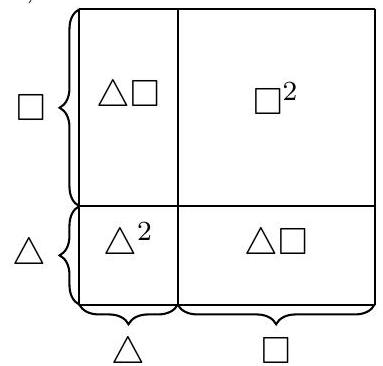
\includegraphics[max width=\textwidth]{2024_11_21_8f01584889ff06348ae7g-103(1)}
\end{center}

Na rysunku widać, że kwadrat o boku długości \(\triangle+\square\), został podzielony na cztery prostokaty o polach \(\triangle^{2}, \triangle \square, \triangle \square, \square^{2}\) czyli jego pole \((\triangle+\square)^{2}=\triangle^{2}+2 \triangle \square+\square^{2}\). Mamy zatem, dla dowolnych \(\triangle, \square\)

\[
(\Delta+\square)^{2}=\triangle^{2}+2 \Delta \square+\square^{2}
\]

\section*{PRZYKŁADY}
W wyrażeniu \((2 x+7)^{2}\) mamy: \(\triangle=2 x\), zaś \(\square=7\), wobec tego

\[
\begin{aligned}
(2 x+7)^{2} & =(2 x)^{2}+2 \cdot 2 x \cdot 7+7^{2} \\
& =4 x^{2}+28 x+49
\end{aligned}
\]

\begin{center}
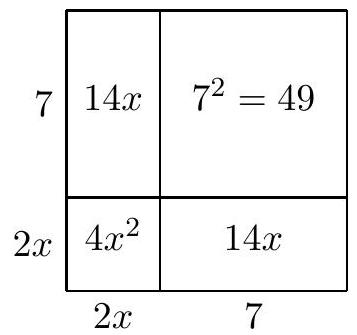
\includegraphics[max width=\textwidth]{2024_11_21_8f01584889ff06348ae7g-103}
\end{center}

Na rysunku widać, że kwadrat o boku długości \(2 x+7\), został podzielony na cztery prostokaty o polach \(4 x^{2}, 14 x, 14 x, 7^{2}\) czyli jego pole \((2 x+7)^{2}=4 x^{2}+28 x+49\)

Podobnie dla \((x+2 y)^{2}\) mamy \(\triangle=x\), zaś \(\square=2 y\), wobec tego

\[
\begin{aligned}
(x+2 y)^{2} & =(x)^{2}+2 \cdot x \cdot 2 y+(2 y)^{2} \\
& =x^{2}+4 x y+4 y^{2}
\end{aligned}
\]

\begin{center}
\begin{tabular}{c|c|c|}
\hline
\(2 y\) & \(2 x y\) & \(4 y^{2}\) \\
\hline
\(x\) &  &  \\
\hline
\multicolumn{2}{|c|}{\(x\)} & \(2 x y\) \\
\hline
\multicolumn{2}{|c|}{\(x\)} & \(2 y\) \\
\hline
\end{tabular}
\end{center}

Na rysunku widać, że kwadrat o boku długości \(x+2 y\), został podzielony na cztery części o polach \(x^{2}, 2 x y, 2 x y, 4 y^{2}\) czyli jego pole jest równe \(x^{2}+4 x y+4 y^{2}\)

I już krótko

\[
(2 x+5 y)^{2}=(2 x)^{2}+2 \cdot 2 x \cdot 5 y+(5 y)^{2}=4 x^{2}+20 x y+25 y^{2}
\]

\begin{enumerate}
  \setcounter{enumi}{24}
  \item Korzystając ze wzoru \((\triangle+\square)^{2}=\triangle^{2}+2 \triangle \square+\square^{2}\) zamień poniższe potęgi na sumy\\
a) \((2+x)^{2}\)\\
b) \((3 x+1)^{2}\)\\
c) \((6 y+2)^{2}\)\\
d) \((4 a+5)^{2}\)\\
e) \((5 x+y)^{2}\)\\
f) \((7 a+1)^{2}\)\\
g) \((2 x+5 y)^{2}\)\\
h) \((x+7 y)^{2}\)\\
i) \((5 x+3)^{2}\)\\
j) \((2 c+5)^{2}\)\\
k) \((a+2 b)^{2}\)\\
l) \((5 x+2)^{2}\)\\
m) \((2 x+1)^{2}\)\\
n) \((x+3)^{2}\)\\
o) \((a+5)^{2}\)\\
p) \((x+2 y)^{2}\)\\
q) \((a+1)^{2}\)\\
r) \((5+y)^{2}\)\\
s) \((3+2 x)^{2}\)\\
t) \((y+10)^{2}\)
\end{enumerate}

Podobnie jak poprzednio, możemy pokazać, że

\[
\begin{aligned}
(\triangle-\square)^{2} & =(\triangle-\square)(\triangle-\square) \\
& =\triangle(\triangle-\square)-\square(\triangle-\square) \\
& =\triangle^{2}-\triangle \square-\triangle \square+\square^{2} \\
& =\triangle^{2}-2 \triangle \square+\square^{2}
\end{aligned}
\]

czyli krótko

\[
(\triangle-\square)^{2}=\triangle^{2}-2 \triangle \square+\square^{2}
\]

\section*{PRZYKŁADY}
W wyrażeniu \((2 a-5)^{2}\) mamy \(\triangle=2 a\), zaś \(\square=5\), wobec tego

\[
\begin{aligned}
(2 a-5)^{2} & =(2 a)^{2}-2 \cdot 2 a \cdot 5+5^{2} \\
& =4 a^{2}-20 a+25
\end{aligned}
\]

Podobnie w wyrażeniu \(\left(3 x-2 y^{2}\right)^{2}\) mamy \(\triangle=3 x, \square=2 y^{2}\), wobec tego mamy

\[
\begin{aligned}
\left(3 x-2 y^{2}\right)^{2} & =(3 x)^{2}-2 \cdot 3 x \cdot 2 y^{2}+\left(2 y^{2}\right)^{2} \\
& =9 x^{2}-12 x y^{2}+4 y^{4}
\end{aligned}
\]

\begin{enumerate}
  \setcounter{enumi}{25}
  \item Korzystając ze wzoru \((\triangle-\square)^{2}=\triangle^{2}-2 \triangle \square+\square^{2}\) zamień poniższe wyrażenia iloczynowe na sumy\\
a) \((7-2 x)^{2}\)\\
b) \((x-2 y)^{2}\)\\
c) \((a-2 b)^{2}\)\\
d) \((4 x-3 y)^{2}\)\\
e) \((a-4)^{2}\)\\
f) \((4-3 a)^{2}\)\\
g) \((2 x-3 a)^{2}\)\\
h) \((y-3)^{2}\)\\
i) \((x-12)^{2}\)\\
j) \((2 a-3)^{2}\)\\
k) \((3 x-4)^{2}\)\\
l) \((5 a-b)^{2}\)\\
m) \((4 x-5)^{2}\)\\
n) \((x-4 a)^{2}\)\\
o) \((x-11)^{2}\)\\
p) \((4-5 y)^{2}\)\\
q) \((3-2 x)^{2}\)\\
r) \((1-3 x)^{2}\)\\
s) \((2 x-y)^{2}\)\\
t) \((2 x y-3)^{2}\)
  \item Korzystając ze wzoru \((\triangle+\square)^{2}=\triangle^{2}+2 \triangle \square+\square^{2}\) lub ze wzoru \((\triangle-\square)^{2}=\triangle^{2}-2 \triangle \square+\square^{2}\) zamień poniższe wyrażenia iloczynowe, w tym przypadku potęgi, na sumy\\
a) \((4+3 r)^{2}\)\\
b) \((5 u+v)^{2}\)\\
c) \((7 x+8 y)^{2}\)\\
d) \((3 b-6)^{2}\)\\
e) \((9-4 y)^{2}\)\\
f) \((2 y-1)^{2}\)\\
g) \((5 x-7 z)^{2}\)\\
h) \(\left(x^{2}+2\right)^{2}\)\\
i) \(\left(2-k^{2}\right)^{2}\)\\
j) \(\left(4 a-b^{2}\right)^{2}\)\\
k) \(\left(u^{2}+v^{2}\right)^{2}\)\\
l) \(\left(x^{2}-3\right)^{2}\)\\
m) \((-x+y)^{2}\)\\
n) \(\left(-2+x^{2}\right)^{2}\)\\
o) \((x y+2)^{2}\)\\
p) \((3-x y)^{2}\)\\
q) \((x y-z)^{2}\)\\
r) \(\left(4 a^{2}+1\right)^{2}\)\\
s) \(\left(1-a x^{2}\right)^{2}\)\\
t) \(\left(a^{2} x-a x^{2}\right)^{2}\)\\
u) \(\left(3 x y^{2}-1\right)^{2}\)\\
v) \(\left(x^{3}-2\right)^{2}\)\\
w) \(\left(y^{4}+1\right)^{2}\)\\
x) \(\left(-p q+r^{2}\right)^{2}\)
\end{enumerate}

Z wzorów (1) i (2) korzystamy również „w przeciwnym kierunku"\\
28. Korzystając ze wzorów \((\triangle+\square)^{2}=\triangle^{2}+2 \triangle \square+\square^{2}\) lub \((\triangle-\square)^{2}=\triangle^{2}-2 \triangle \square+\square^{2}\) zamień poniższe sumy algebraiczne na kwadraty odpowiednich wyrażeń\\
a) \(x^{2}-2 x y+y^{2}=\)\\
b) \(a^{2}+4 a+4=\)\\
c) \(a^{2}+6 a+9=\)\\
d) \(y^{2}-16 y+64=\)\\
e) \(x^{2}-2 x+1=\)\\
f) \(9-6 x+x^{2}=\)\\
g) \(a^{2}-4 a y+4 y^{2}=\)\\
h) \(y^{2}-10 a y+25 a^{2}=\)\\
i) \(4 y^{2}-24 x y+36 x^{2}=\)\\
j) \(25 a^{2}-20 a b+4 b^{2}=\)\\
k) \(49 x^{2}-56 x y+16 y^{2}=\)

\begin{enumerate}
  \item \(100 a^{2}-180 a b+81 b^{2}=\)\\
m) \(x^{2}+14 x y+49 y^{2}=\)\\
n) \(4 a^{2}+8 a b+4 b^{2}=\)\\
o) \(25 x^{2}+20 x y+4 y^{2}=\)\\
p) \(100 y^{2}+60 a y+9 a^{2}=\)\\
q) \(a^{2}+6 a b+9 b^{2}=\)\\
r) \(x^{2}+8 x y+16 y^{2}=\)\\
s) \(16 a^{2}+72 a b+81 b^{2}=\)\\
t) \(x^{2}+12 x+36=\)\\
u) \(16 a^{2}-40 a x+25 x^{2}=\)\\
v) \(4+32 a^{2}+64 a^{4}=\)\\
w) \(x^{4}+14 x^{2}+49=\)\\
x) \(25+10 y^{2}+y^{4}=\)\\
y) \(x^{6}+18 x^{3}+81=\)\\
z) \(81-72 t^{2}+16 t^{4}=\)
\end{enumerate}

Zauważmy, że ma miejsce następujący wzór: \((\triangle+\square)(\triangle-\square)=\triangle^{2}-\square^{2}\). Faktycznie

\[
\begin{aligned}
(\triangle+\square)(\triangle-\square) & =\triangle(\triangle-\square)+\square(\triangle-\square) \\
& =\triangle^{2}-\triangle \square+\square \triangle-\square^{2} \\
& =\triangle^{2}-\square^{2}
\end{aligned}
\]

czyli krótko dla dowolnego \(\triangle \mathrm{i}\)

\[
(\triangle+\square)(\triangle-\square)=\triangle^{2}-\square^{2}
\]

Z wzoru tego korzystamy na dwa sposoby albo zamieniając iloczyn na sumę jak w kolejnym zadaniu, albo też sumę na iloczyn jak w następnym zadaniu. PRZYKŁADY zamiany iloczynu na sumę algebraiczną.

\[
\begin{aligned}
(4 a-3 b)(4 a+3 b) & =(4 a)^{2}-(3 b)^{2} \\
& =16 a^{2}-9 b^{2} \\
\left(x-2 y^{2}\right)\left(x+2 y^{2}\right) & =x^{2}-\left(2 y^{2}\right)^{2} \\
& =x^{2}-4 y^{4}
\end{aligned}
\]

\begin{enumerate}
  \setcounter{enumi}{28}
  \item Korzystając z wzoru \((\triangle+\square)(\triangle-\square)=\triangle^{2}-\square^{2}\) zamień poniższe iloczyny na sumy\\
a) \((3-a)(3+a)\)\\
b) \((a+4)(a-4)\)\\
c) \((2 a+b)(2 a-b)\)\\
d) \((5 x-2 y)(5 x+2 y)\)\\
e) \(\left(x^{2}-1\right)\left(x^{2}+1\right)\)\\
f) \((2 x-1)(2 x+1)\)\\
g) \((a-b)(a+b)\)\\
h) \((2 x-1)(1+2 x)\)\\
i) \((3 x+1)(3 x-1)\)\\
j) \((5 a+b)(5 a-b)\)\\
k) \((4 a+2 y)(4 a-2 y)\)
\end{enumerate}

\begin{enumerate}
  \item \((x-3 y)(x+3 y)\)\\
m) \((3 a-5 b)(3 a+5 b)\)\\
n) \((4 a+7 b)(4 a-7 b)\)\\
o) \((2 x-11)(11+2 x)\)\\
p) \((5 x-4)(5 x+4)\)\\
q) \((12 a+1)(12 a-1)\)\\
r) \((9 y-5 x)(9 y+5 x)\)\\
s) \((7 x-8 b)(7 x+8 b)\)\\
t) \(\left(9 x-6 y^{2}\right)\left(9 x+6 y^{2}\right)\)\\
u) \((x y-1)(x y+1)\)\\
v) \(\left(a^{2}-y^{2}\right)\left(a^{2}+y^{2}\right)\)\\
w) \(\left(x^{2} y+b^{3}\right)\left(x^{2} y-b^{3}\right)\)\\
x) \(\left(x^{3}-b\right)\left(x^{3}+b\right)\)
\end{enumerate}

PRZYKŁADY zamiany sumy algebraicznej na iloczyn.

\[
\begin{aligned}
9 a^{2}-16 b^{2} & =(3 a)^{2}-(4 b)^{2} \\
& =(3 a-4 b)(3 a+4 b) \\
1-25 x^{4} & =1^{2}-\left(5 x^{2}\right)^{2} \\
& =\left(1-5 x^{2}\right)\left(1+5 x^{2}\right)
\end{aligned}
\]

\begin{enumerate}
  \setcounter{enumi}{29}
  \item Korzystając ze wzoru \((\triangle+\square)(\triangle-\square)=\triangle^{2}-\square^{2}\) zamień poniższe sumy na iloczyny\\
a) \(x^{2}-4\)\\
b) \(x^{2}-1\)\\
c) \(x^{2}-9\)\\
d) \(y^{2}-16\)\\
e) \(25-x^{2}\)\\
f) \(16-y^{2}\)\\
g) \(4 x^{2}-49\)\\
h) \(1-9 x^{2}\)\\
i) \(9-16 x^{2}\)\\
j) \(49 a^{2} b^{2}-64 y^{2}\)\\
k) \(4 a^{2}-36\)\\
l) \(36-81 x^{2}\)\\
m) \(64-9 y^{4}\)\\
n) \(-81+16 a^{4}\)\\
o) \(-100+81 x^{6}\)\\
p) \(121 x^{2}-4 u^{4}\)\\
q) \(25 y^{2}-49 x^{8}\)\\
r) \(144 a^{2}-16 y^{4}\)\\
s) \(25 x^{2}-144 a^{6}\)\\
t) \(169 y^{2}-9 a^{4}\)\\
u) \(144 x^{12}-121 b^{4}\)\\
v) \(9-36 x^{4}\)\\
w) \(169 b^{2}-9 c^{4}\)\\
x) \(16 y^{6}-49 x^{4}\)\\
y) \(25 x^{4} y^{2}-9 z^{6}\)\\
z) \(4 x^{6} y^{2}-81 z^{4}\)
\end{enumerate}

\section*{Odpowiedzi.}
\begin{enumerate}
  \item a) \(a+b\), b) \(a^{2}+b^{2}\), c) \(a^{3}+b^{3}\), d) \(a^{3}-b^{3}\), e) \(\frac{1}{a-b}\), f) \(\frac{1}{a^{3}+b^{3}}\), g) \(\frac{1}{a^{2}+b^{2}}\), h) \(\frac{1}{a}+\frac{1}{b}\), i) \(\frac{1}{a^{2}}+\frac{1}{b^{2}}\), j) \(\frac{1}{a^{3}}-\frac{1}{b^{3}}\), k) \((a-b)^{2}\), l) \((x-y)^{3}\), m) \(\left(a^{2}+b^{2}\right)^{2}\), n) \(\left(\frac{1}{a+b}\right)^{2}\), o) \(\left(\frac{1}{a}+\frac{1}{b}\right)^{2}\), p) \(\left(\frac{1}{a^{2}-b^{2}}\right)^{2}\), q) \(\frac{1}{\frac{1}{a}+\frac{1}{b}}\),\\
r) \(\left(a^{2}-b^{2}\right)^{3}\),
  \item a) \(\left(10^{3}\right)^{2}\), b) \(\left(a^{3}+b^{3}\right) \cdot\left(m^{2}+n^{2}\right)^{2}\), c) \(\left(\frac{1}{m}\right)^{3}+\left(\frac{1}{n}\right)^{3}\), d) \(\frac{a^{2}+b^{2}}{(a-b)^{2}}\), e) \(\left(2^{100}+2^{50}\right)^{2}\), f) \(a+b^{2}\), g) \(b^{3}-4\), h) \(\frac{a^{2}}{5}\), i) \(-2 a^{2} b^{3}\), j) \(2 a(x+y)^{2}\), k) \(\frac{a^{2}-b^{2}}{c^{3}}\)
  \item a) suma liczb \(a, b\) i \(c\) b) odwrotność sumy liczb \(x\) i \(y\) c) odwrotność sumy liczby \(x\) i kwadratu liczby \(y \mathrm{~d}\) ) suma odwrotności kwadratu liczby \(x\) i sześcianu liczby \(y\) e) odwrotność sumy sześcianu liczby \(a\) i kwadratu liczby \(b \mathrm{f}\) ) odwrotność różnicy liczby \(a\) i sześcianu liczby \(x \mathrm{~g}\) ) odwrotność kwadratu sumy liczb \(a\) i \(b\) h) odwrotność kwadratu różnicy sześcianu liczby \(a\) i kwadratu liczby \(b\) i) różnica odwrotności sześcianu liczby \(a\) i kwadratu liczby \(b\) j) suma sześcianu liczby \(a\) i kwadratu liczby \(b\) k) różnica sześcianów liczb \(x\) i \(y\) l) sześcian sumy liczb \(x, y\) i \(z \mathrm{~m}\) ) iloczyn sumy liczb \(a\) i \(b\) przez różnicę kwadratów liczb \(x\) i \(y\) n) iloczyn różnicy liczb \(a\) i \(b\) przez sumę sześcianów liczb \(x\) i \(y\) o) iloczyn różnicy kwadratów liczb \(a\) i \(b\) przez sumę kwadratów liczb \(a\) i \(b\)
  \item a) \(n-2\) b) \(n+3\) c) \(3 n\) d) \(n, n+1, n+2\) e) \(n^{2}+1\) f) \((n+1)^{3}\)
  \item a) \(2 k+1,2 k+3,2 k+5\), b) \(2 k, 2 k+2,2 k+4\), c) \(2 k-4,2 k-2,2 k\)
  \item a) \(10(x-7)+x\) b) \(100 x+10 \cdot 4+x\) c) \(100 \cdot(2 x+2)+10 \cdot 2 x+x\)\\
d) \(100(x+2)+10(x+1)+x\) e) \(10 \cdot 2 x+x\) f) \(100 \cdot 3(x-3)+10 x+x-3\)
  \item a) \(2 x\)-wiek Bartka, \(x+2\) wiek Cześka b) \(2 x-4\) c) \(x+7\) d) \(2 x+2\)
  \item \(\frac{1}{2} \cdot \frac{1}{4} x\)
  \item a) \(x-\frac{1}{2}, y+\frac{1}{2}\),\\
b) \(\frac{1}{2} x+2, \frac{1}{2} x+y-2\),\\
c) \(\frac{2}{3} x+\frac{1}{2}, y+\frac{1}{3} x+\frac{1}{4}\), d) \(\frac{3}{4} x+\frac{1}{2} y\),
  \item a) \(5 a\), b) \(10 b^{2}\), c) \(-5 x^{2} z\), d) \(-7 \frac{1}{6} x\), e) \(9 a-7 b\), f) \(9 a-b^{2}\), g) \(6 \frac{5}{6} a\), h) \(12 x y\), i) \(-7 x^{2} z-x z\), j) \(x y+3 x+y\), k) \(10 \frac{1}{2} a b-3 a-6 b\), l) \(47 x-58 x y\), m) \(7 x^{2} y+2 x^{3} z-3 x y^{2}\), n) \(8 a b-8 a^{2} b^{2}-9 a b^{2}\),
  \item a) \(\frac{1}{2} x\) b) \(\frac{1}{20} x\) c) \(\frac{1}{5} x\) d) \(\frac{1}{2} x\) e) \(x\) f) \(\frac{3}{5} x\)
  \item a) \(2 a+4 b-3\), b) \(-a+3 b\), c) \(2 a+6 b-2\), d) \(14 a+3 b-7 c\), e) \(x-3 y+17\), f) \(5 x+5 y+8\), g) \(5 b^{2}-12 a\), h) \(a+2 b+3 c\),
  \item a) \(5 x^{2}+4 y^{2}+2 y\), b) \(3 x^{2}+y^{2}+3 z\), c) \(3 x^{2}-4 x y+3 y\), d) \(-6 x+4 y-20\), e) \(-x-8\), f) \(y^{2}-3\), g) \(2 x^{2}+3\), h) \(-12,2 y+31\), i) \(-11 y^{2}-7 y\)
  \item a) \(2 x+6 y\), b) \(4 x+8 y^{2}\), c) \(15 x-10 x y\), d) \(-8 x-20 y\), e) \(-20 x y^{2}+15\), f) \(6 x-4 y^{2}\), g) \(20 x^{2}-15 y\), h) \(15 x-10 y^{2}\), i) \(-6 x-8 y\), j) \(-10 x+5 y\),\\
k) \(14 x+35 y\), l) \(8 x^{2}+12 x y\), m) \(4 x^{2} y^{3}+2 x^{4} y^{3}\), n) \(3 x^{2} y^{3}-5 x^{4} y^{4}\),\\
o) \(-10 x^{2}-15 x y\), p) \(-4 x^{4} y^{2}+6 x y^{4}\),
  \item a) \(2 x+6 y-14\), b) \(2 x^{2}+6 x^{4} y^{2}-4 x y\), c) \(8 x^{3} y-4 x^{2} y-8 x y^{2}\),\\
d) \(-6 x+10 y+14 x^{4}\), e) \(-6 x^{2}+9 y+15\), f) \(3 x^{3} y^{2}-6 x^{2} y^{3}+3 x y^{3}\),\\
g) \(6 x^{2} y z+2 x y z-4 y^{3} z\), h) \(3 x^{3} z+3 x^{2} y z-3 x y^{2} z\), i) \(-4 x^{3} y^{2} z^{4}+8 x^{3} y z^{4}+2 x^{2} y z^{5}\),\\
j) \(\left.-8 a^{3} b^{3}+2 a^{3} b^{2}+6 a^{5} b^{2}, \mathrm{k}\right)-8 x y+12 y^{2}+4 y^{3}\), l) \(-6 x^{2} y+8 x^{3} z+4 x^{2} z^{2}\),\\
m) \(\left.-3 x^{2}-6 x y+15 x, \mathrm{n}\right)-12 y^{5}+8 x y^{5}-4 x^{2} y^{4}\), о) \(-24 x^{2} z^{2}+18 x y^{2} z^{2}+12 x z^{3}\),\\
p) \(-24 x^{2} y^{2}+18 x y^{4}-12 x y^{2} z^{2}\),
  \item a) \(-6 x\) b) \(33 u^{2}-5 u w\) c) \(7 p^{3}-22 p^{2}\) d) \(a^{2}+b^{2}+c^{2}\) e) \(a b c-2 x y z\) f) \(3 x^{2} y-3 x y^{2}\) g) \(x y z^{2}\)
  \item a) \(4 x-7 z\) b) \(-2 a b+19 x\) c) \(0,5 a^{2}-0,3 a+0,7\) d) \(-5 a^{2}+9 p\) e) \(-18 x^{2}+\) \(72 x-36\) f) \(-x^{2}-3 x y\)
  \item a) \(x-12 y\) b) \(x+2 y\) c) \(-4 x+9 y\) d) \(3 x^{3}-2 x^{2}+4 x\) e) \(10 \frac{1}{3} b^{2}-17 \frac{1}{3} b\)
  \item a) \(a(17+b)\), b) \(b(3 a+7-12 b)\), c) \(6 b\left(2+3 b-4 b^{2}\right)\), d) \(4 x^{2} y(3-5 x+4 y)\),\\
e) \(5 a b\left(4 b+2 a^{2} b^{2}-5\right)\),\\
f) \(5 x^{2} y\left(3 x y+2-4 y^{2}\right)\), g) \(9 x(2 b x y-3 a-4 a x)\), h) \(4 a x\left(1-2 x-3 x^{2}\right)\),\\
i) \(-a^{3}\left(4 y+15 a b^{2}-20 b^{4}\right)\), j) \(12 x^{2} y^{2}\left(5 x-y-3 x^{2}\right)\)
  \item a) \(a(a+b)\), b) \(a(2+a)\), c) \(a b(a+b)\), d) \(x(4 x+1)\), e) \(a^{2}(a-1)\),\\
f) \(3(2 x-y+3 z)\), g) \(2 x(4 y-3 x+1)\), h) \(3 x\left(4 x^{2}-2 x+1\right)\),\\
i) \(3 x\left(x+27 x^{2} y-9 y^{2}\right)\), j) \(a^{2}\left(a^{2}-1\right)\), k) \(3 a^{2}(1-4 a)\), l) \(3 b^{3}(6 a-5 b)\),\\
m) \(3 x^{3}(3 x-4 y)\), n) \(2 a b^{2}(4 a b-5)\), о) \(3 x^{2} y^{2}(x y+4)\),\\
p) \(7 a^{4}\left(3+2 a b^{2}-a^{3} b^{5}\right)\), q) \(-7 x^{2}\left(3 x^{3}+5\right)\), r) \(4\left(6 a^{2}-8 a+15\right)\),\\
s) \(a\left(a^{2} b+b+c\right)\), t) \(a b\left(a^{2}+a b+b^{2}\right)\), u) \(2 x^{3}\left(2 x^{2}-3 x-4\right)\), v) \(9 a b(4 a-5 b-1)\),
  \item a) \(x+6\) b) \(-3 a+4 b\) c) \(2 a-4\) d) \(4 x-11\)
  \item a) \(a c+b c+a d+b d\), b) \(2 a c+2 a^{2}-b c-a b\), c) \(a^{2}+2 a b+b^{2}\), d) \(a^{2}-b^{2}\),\\
e) \(3 x y-6 x z-y^{2}+2 y z\), f) \(a^{2}+4 a b+3 b^{2}\), g) \(a^{2}-a-6\), h) \(b^{2}+1,5 b-10\),\\
i) \(2 a b+3 a c-2 b^{2}-3 b c\), j) \(\left.c^{2}+7 c+10, \mathrm{k}\right) a x-a y+b x-b y\), l) \(2 u^{2}-u v-3 v^{2}\),\\
m) \(2 r^{2}-5 r s+2 s^{2}\), n) \(9 p-6 p^{2}-6 q+4 p q\),\\
o) \(-6 x^{2}+10 x y+4 y^{2}\), p) \(16 a^{2}-25 b^{2}\), q) \(-a^{3}+2 a^{2}-3 a+6\), r) \(a^{3}+a b-\) \(a^{2} b^{2}-b^{3}\), s) \(c^{3}-c e+c^{2} d^{2}-d^{2} e\), t) \(f^{4}-e^{4}\), u) \(12 p q+4 p^{3}-9 q^{3}-3 p^{2} q^{2}\), v) \(3 p^{5}+p^{3} q^{3}-6 p^{2} q^{2}-2 q^{5}\), w) \(x^{2} y z+x y^{2}+x z^{2}+y z\)
  \item a) \(a x+a y-b x-b y+x+y\), b) \(a x+a y-a+2 b x+2 b y-2 b\),\\
c) \(6 a^{2}+11 a b-24 a c+4 b^{2}-32 b c\), d) \(15 x+24 x y-10 x^{2}-6 y-8 y^{2}\),\\
e) \(a^{2}+4 a-b^{2}+2 b+3\), f) \(a^{2}-b^{2}-c^{2}+2 b c\), g) \(c^{2}-d^{2}-2 d e-e^{2}\), h) \(-c^{2}-d^{2}-e^{2}-2 c d-2 c e-2 d e\), i) \(8 p^{2}+14 p r-2 q^{2}+9 q r-4 r^{2}\), j) \(\left.r^{3}+1, \mathrm{k}\right) s^{4}+s^{2}+1\)
  \item a) \((x+y)(a+b)\) b) \((2-3 x)(a-b)\) c) \(10 m(k-1)\) d) \((a-1)\left(3 x^{2}-x+1\right)\) e) \((x-2)\left(y^{2}-y-1\right)\)
  \item a) \(x^{2}+4 x+4\), b) \(9 x^{2}+6 x+1\), c) \(36 y^{2}+24 y+4\), d) \(16 a^{2}+40 a+25\),\\
e) \(25 x^{2}+10 x y+y^{2}\), f) \(49 a^{2}+14 a+1\), g) \(4 x^{2}+20 x y+25 y^{2}\),\\
h) \(x^{2}+14 x y+49 y^{2}\), i) \(25 x^{2}+30 x+9\), j) \(4 c^{2}+20 c+25\), k) \(a^{2}+4 a b+4 b^{2}\),\\
l) \(25 x^{2}+20 x+4\), m) \(4 x^{2}+4 x+1\), n) \(x^{2}+6 x+9\), o) \(a^{2}+10 a+25\),\\
p) \(x^{2}+4 x y+4 y^{2}\), q) \(a^{2}+2 a+1\), r) \(25+10 y+y^{2}\), s) \(9+12 x+4 x^{2}\),\\
t) \(y^{2}+20 y+100\),
  \item a) \(49-28 x+4 x^{2}\), b) \(x^{2}-4 x y+4 y^{2}\), c) \(a^{2}-4 a b+4 b^{2}\), d) \(16 x^{2}-24 x y+9 y^{2}\), e) \(a^{2}-8 a+16\), f) \(16-24 a+9 a^{2}\), g) \(4 x^{2}-12 a x+9 a^{2}\), h) \(y^{2}-6 y+9\), i) \(x^{2}-24 x+144\), j) \(4 a^{2}-12 a+9\), k) \(9 x^{2}-24 x+16\), l) \(25 a^{2}-10 a b+b^{2}\), m) \(16 x^{2}-40 x+25\), n) \(x^{2}-8 a x+16 a^{2}\), o) \(x^{2}-22 x+121\), p) \(16-40 y+25 y^{2}\), q) \(9-12 x+4 x^{2}\), r) \(1-6 x+9 x^{2}\), s) \(4 x^{2}-4 x y+y^{2}\), t) \(4 x^{2} y^{2}-12 x y+9\),
  \item a) \(16+24 r+9 r^{2}\), b) \(25 u^{2}+10 u v+v^{2}\), c) \(49 x^{2}+112 x y+64 y^{2}\),\\
d) \(9 b^{2}-36 b+36\), e) \(81-72 y+16 y^{2}\), f) \(4 y^{2}-4 y+1\), g) \(25 x^{2}-70 x z+49 z^{2}\), h) \(x^{4}+4 x^{2}+4\), i) \(4-4 k^{2}+k^{4}\), j) \(16 a^{2}-8 a b^{2}+b^{4}\), k) \(u^{4}+2 u^{2} v^{2}+v^{4}\), l) \(\left.x^{4}-6 x^{2}+9, \mathrm{~m}\right) x^{2}-2 x y+y^{2}\), n) \(4-4 x^{2}+x^{4}\), о) \(x^{2} y^{2}+4 x y+4\), p) \(9-6 x y+x^{2} y^{2}\), q) \(x^{2} y^{2}-2 x y z+z^{2}\), r) \(16 a^{4}+8 a^{2}+1\), s) \(1-2 a x^{2}+a^{2} x^{4}\), t) \(a^{4} x^{2}-2 a^{3} x^{3}+a^{2} x^{4}\), u) \(9 x^{2} y^{4}-6 x y^{2}+1\), v) \(x^{6}-4 x^{3}+4\), w) \(y^{8}+2 y^{4}+1\), x) \(p^{2} q^{2}-2 p q r^{2}+r^{4}\)
  \item a) \((x-y)^{2}\), b) \((a+2)^{2}\), c) \((a+3)^{2}\), d) \((y-8)^{2}\), e) \((x-1)^{2}\), f) \((3-x)^{2}\),\\
g) \(\left.(a-2 y)^{2}, \mathrm{~h}\right)(y-5 a)^{2}\), i) \((2 y-6 x)^{2}\), j) \((5 a-2 b)^{2}\),\\
k) \((7 x-4 y)^{2}\), l) \((10 a-9 b)^{2}\), m) \((x+7 y)^{2}\), n) \((2 a+2 b)^{2}\), o) \((5 x+2 y)^{2}\),\\
p) \((10 y+3 a)^{2}\), q) \((a+3 b)^{2}\), r) \((x+4 y)^{2}\), s) \((4 a+9 b)^{2}\), t) \((x+6)^{2}\),\\
u) \((4 a-5 x)^{2}\), v) \(\left(2+8 a^{2}\right)^{2}\), w) \(\left(x^{2}+7\right)^{2}\), x) \(\left(5+y^{2}\right)^{2}\) y) \(\left.\left(x^{3}+9\right)^{2} \mathrm{z}\right)\) \(\left(9-4 t^{2}\right)^{2}\)
  \item a) \(9-a^{2}\), b) \(a^{2}-16\), c) \(4 a^{2}-b^{2}\), d) \(25 x^{2}-4 y^{2}\), e) \(x^{4}-1\), f) \(4 x^{2}-1\), g) \(a^{2}-b^{2}\), h) \(4 x^{2}-1\), i) \(9 x^{2}-1\), j) \(25 a^{2}-b^{2}\), k) \(16 a^{2}-4 y^{2}\), l) \(x^{2}-9 y^{2}\), m) \(9 a^{2}-25 b^{2}\), n) \(16 a^{2}-49 b^{2}\), о) \(4 x^{2}-121\), p) \(25 x^{2}-16\), q) \(144 a^{2}-1\), r) \(81 y^{2}-25 x^{2}\), s) \(49 x^{2}-64 b^{2}\), t) \(81 x^{2}-36 y^{4}\), u) \(x^{2} y^{2}-1\), v) \(a^{4}-y^{4}\), w) \(x^{4} y^{2}-b^{6}\), x) \(x^{6}-b^{2}\),
  \item a) \((x-2)(x+2)\), b) \((x-1)(x+1)\), c) \((x-3)(x+3)\), d) \((y-4)(y+4)\),\\
e) \((5-x)(5+x)\), f) \((4-y)(4+y)\), g) \((2 x-7)(2 x+7)\), h) \((1-3 x)(1+3 x)\),\\
i) \((3-4 x)(3+4 x)\), j) \((7 a b-8 y)(7 a b+8 y)\), k) \((2 a-6)(2 a+6)\),\\
l) \((6-9 x)(6+9 x), \mathrm{m})\left(8-3 y^{2}\right)\left(8+3 y^{2}\right)\), n) \(\left(4 a^{2}-9\right)\left(4 a^{2}+9\right)\),\\
o) \(\left.\left(9 x^{3}-10\right)\left(9 x^{3}+10\right), \mathrm{p}\right)\left(11 x-2 u^{2}\right)\left(11 x+2 u^{2}\right)\), q) \(\left(5 y-7 x^{4}\right)\left(5 y+7 x^{4}\right)\),\\
r) \(\left(12 a-4 y^{2}\right)\left(12 a+4 y^{2}\right)\), s) \(\left(5 x-12 a^{3}\right)\left(5 x+12 a^{3}\right)\),\\
t) \(\left(13 y-3 a^{2}\right)\left(13 y+3 a^{2}\right)\), u) \(\left(12 x^{6}-11 b^{2}\right)\left(12 x^{6}+11 b^{2}\right)\),\\
v) \(\left(3-6 x^{2}\right)\left(3+6 x^{2}\right)\), w) \(\left.\left(13 b-3 c^{2}\right)\left(13 b+3 c^{2}\right) \mathrm{x}\right)\left(4 y^{3}-7 x^{2}\right)\left(4 y^{3}+7 x^{2}\right)\)\\
y) \(\left(5 x^{2} y-3 z^{3}\right)\left(5 x^{2} y+3 z^{3}\right)\) z) \(\left(2 x^{3} y-9 z^{2}\right)\left(2 x^{3} y+9 z^{2}\right)\)
\end{enumerate}

\section*{Rozdział 6}
\section*{RÓWNANIA}
Obecnie będziemy się zajmować równaniami. Będą to równania, w których występuje tylko jedna niewiadoma. Na początku zajmiemy się równaniami, które mają tylko jedno rozwiązanie. Oznacza to, że tylko jedna liczba wstawiona w miejsce niewiadomej spełnia to równanie. Liczbę, która spełnia dane równanie nazywamy rozwiązaniem równania, albo pierwiastkiem równania.

\subsection*{6.1 Rozwiązanie równania}
\section*{PRZYKŁAD 1}
Liczba 3 jest pierwiastkiem równania

\[
x-3=0,
\]

bo gdy za \(x\) wstawimy 3 , to mamy wówczas:

\[
3-3=0
\]

czyli

\[
0=0
\]

co jest prawdą. Zatem liczba 3, nazwijmy ją sobie \(x_{0}\), jest rozwiązaniem równania \(x-3=0\). Piszemy to krócej: rozwiązaniem równania jest \(x_{0}=3\). Będziemy też pisali \(Z R=\{3\}\), co oznacza, że jedynym elementem zbioru rozwiązań równania jest liczba 3.

\section*{PRZYKŁAD 2}
Liczba -8 jest pierwiastkiem równania

\[
2 C-1=3(C+1)+4
\]

bo gdy za \(C\) wstawimy liczbę -8 , to mamy wówczas

\[
\begin{aligned}
2(-8)-1 & =3(-8+1)+4 \\
-16-1 & =3(-7)+4 \\
-17 & =-21+4 \\
-17 & =-17
\end{aligned}
\]

co jest prawdą. Zatem faktycznie liczba -8 jest pierwiastkiem równania \(2 C-1=3(C+1)+4\).

\section*{PRZYKŁAD 3}
Liczba -3 jest pierwiastkiem równania

\[
(\Delta+7)^{2}-(\Delta+3)(\Delta-3)-16=0
\]

bo gdy za \(\Delta\) wstawimy -3 , to wykonując kolejne działania mamy:

\[
\begin{aligned}
(-3+7)^{2}-(-3+3)(-3-3)-16 & =0 \\
4^{2}-0 \cdot(-6)-16 & =0 \\
16-0-16 & =0 \\
0 & =0
\end{aligned}
\]

co jest prawdą. Zatem liczba -3 jest pierwiastkiem równania \((\Delta+7)^{2}-(\Delta+3)(\Delta-3)-16=0\), czyli \(Z R=\{-3\}\).

\subsection*{6.2 Rozwiązywanie równań}
Rozwiązywanie równania jest to proces polegający na przekształcaniu równania do takiej postaci, z której możemy łatwo orzec jaka liczba jest pierwiastkiem tego wyjściowego równania. Zanim jednak zajmiemy się przekształcaniem równań, spróbujmy najpierw rozwiązać w pamięci poniższe równania:

Równanie\\
\(x=2\)\\
\(y+3=9\)\\
\(2 x=6\)\\
\(2 b+1=9 \quad\) czyli \(\quad 2 b=8\)\\
\(\frac{x-2}{7}=2 \quad\) czyli \(\quad x-2=14\)

\begin{enumerate}
  \item Rozwiąż w pamięci równania\\
a) \(x+3=10\)\\
b) \(y+4=10\)\\
c) \(x-3=7\)\\
d) \(x-\frac{1}{2}=5 \frac{1}{2}\)\\
e) \(y+2 \frac{1}{2}=7\)\\
f) \(x+2 \frac{1}{3}=5\)\\
g) \(x-7=-5\)\\
h) \(y-3 \frac{1}{2}=1 \frac{1}{2}\)\\
i) \(x-3 \frac{1}{3}=\frac{2}{3}\)\\
j) \(\frac{x+3}{4}=2\)\\
k) \(\frac{y-3}{2}=5\)\\
l) \(\frac{x+1}{3}=1\)
\end{enumerate}

Na ogół rozwiązywanie równania polega na przekształceniu go do postaci

\[
x=l i c z b a \quad \text { na przykład } \quad x=2 \frac{1}{2}
\]

\section*{PRZYKŁAD 1}
Rozwiążmy równanie

\[
2 x+5=12
\]

Łatwo sprawdzić, że liczba \(\frac{7}{2}\) spełnia to równanie. Liczba ta również spełnia równanie

\[
2 x+5-5=12-5 \quad(\text { od obu stron równania odjęliśmy } 5)
\]

otrzymując równanie

\[
2 x=7
\]

Liczba \(\frac{7}{2}\) spełnia to równanie, wobec tego spełnia ona również równanie\\
\(\frac{1}{2} \cdot 2 x=\frac{1}{2} \cdot 7 \quad\) (obie strony równania pomnożyliśmy przez \(\frac{1}{2}\) )\\
otrzymując równanie

\[
x=\frac{7}{2}
\]

którego rozwiązaniem jest liczba \(\frac{7}{2}\) czyli \(Z R=\left\{\frac{7}{2}\right\}\).

\section*{PRZYKŁAD 2}
Niech dane będzie równanie:

\[
2 x-1=3 x+4
\]

Łatwo sprawdzić, że liczba -5 spełnia to równanie. Wobec tego ta liczba spełnia również równanie

\[
2 x-1-3 x=3 x+4-3 x \quad(\text { od obu stron odjęliśmy } 3 x)
\]

czyli równanie

\[
-x-1=4
\]

czyli równanie

\[
-x=5 \quad(\text { do obu stron dodaliśmy } 1)
\]

czyli równanie

\[
x=-5 . \quad \text { (obie strony pomnożykiśmy przez }-1)
\]

Liczba -5 , spełnia to równanie, bo gdy wstawimy ją za \(x\), to dostaniemy równość \(-5=-5\), co jest prawdą. Zatem \(Z R=\{-5\}\).

Rozwiązania równania nie zmieniają następujące operacje:

\begin{itemize}
  \item Dodanie/odjęcie do/od obu stron równania takiego samego wyrażenia.
  \item Pomnożenie/podzielenie obu stron równania przez taką sama liczbę (różną od 0).
\end{itemize}

\begin{enumerate}
  \setcounter{enumi}{1}
  \item Dokonując odpowiednich przekształceń rozwiąż równania:\\
a) \(9 x+7=3 x-11\)\\
b) \(2 x+7=29-2 x\)\\
c) \(3-7 x=4 x-19\)\\
d) \(5 x+7=3 x+18\)\\
e) \(6 x-15=3 x-9\)\\
f) \(2(x+6)=28-2 x\)\\
g) \(12 x-7=3 x+20\)\\
h) \(2(x+2)=5(x-1)\)\\
i) \(3 x-2=11 x+20\)
\end{enumerate}

\section*{PRZYKŁAD 3}
Rozwiąż równanie

\[
\begin{aligned}
x-7-(6 x+10) & =3 \\
x-7-6 x-10 & =3 \\
-5 x-17 & =3 \\
-5 x-17+17 & =3+17 \\
-5 x & =20 \\
\text { czyli } & \\
x & =-4
\end{aligned}
\]

Odpowiedź: \(Z R=\{-4\}\)

\section*{PRZYKŁAD 4}
\[
\begin{aligned}
7 x-(9-3 x) & =12 x+3(x+2) \\
7 x-9+3 x & =12 x+3 x+6 \\
10 x-9 & =15 x+6 \\
10 x & =15 x+6+9 \quad \mid+9 \\
-5 x & =15 \quad \mid-15 x \\
-15 & =5 x \\
\text { czyli } & \\
x & =-3
\end{aligned}
\]

\begin{enumerate}
  \setcounter{enumi}{2}
  \item Rozwiąż równania:\\
a) \(1-(4-3 x)=5 x+3\)\\
b) \(7-(3-5 x)=2 x-(4 x+3)\)\\
c) \(2 x+5-(4 x-2)=10-(5 x-23)\)\\
d) \(2 x+3-(6-5 x)=3 x+7\)\\
e) \(5(x-2)+2(3 x-7)=2 x-(3 x+8)\)\\
f) \(5 x=2(7-2 x)-(2-3 x)\)\\
g) \(7(3-2 x)-(3-4 x)=2 x-(4 x+6)\)\\
h) \(8 x-(3 x+2)=2 x+16\)\\
i) \(4(3 x-1)-(2 x-1)=x-(7 x-3)\)\\
j) \(7+3 x=4 x-(2 x-2)\)\\
k) \(3(x+1)-(x-2)=12 x-5\)\\
l) \(4 x-(2-x)=2(5 x+4)\)
\end{enumerate}

Dane równanie można rozwiązywać zazwyczaj na różne sposoby.

\section*{PRZYKŁAD 5}
\section*{I sposób}
\[
\begin{aligned}
\frac{2 x-7}{3}+\frac{3 x+1}{2} & =2 \\
\frac{2}{3} x-\frac{7}{3}+\frac{3}{2} x & +\frac{1}{2}=2 \\
\frac{2}{3} x+\frac{3}{2} x & =2+\frac{7}{3}-\frac{1}{2} \\
\frac{4}{6} x+\frac{9}{6} x & =\frac{12}{6}+\frac{14}{6}-\frac{3}{6} \\
\frac{13}{6} x & =\frac{23}{6} \\
x=\frac{23}{6} \cdot \frac{6}{13} & =\frac{23}{13}=1 \frac{10}{13}
\end{aligned}
\]

II sposób

\[
\begin{aligned}
& \frac{2 x-7}{3}+\frac{3 x+1}{2}=2 \\
& 6 \cdot\left[\frac{2 x-7}{3}+\frac{3 x+1}{2}\right]=6 \cdot 2 \\
& 6 \cdot \frac{2 x-7}{3}+6 \cdot \frac{3 x+1}{2}=12 \\
& \frac{6 \cdot(2 x-7)}{3}+\frac{6 \cdot(3 x+1)}{2}=12 \\
& 2(2 x-7)+3(3 x+1)=12 \\
& 4 x-14+9 x+3=12 \\
& 13 x=23 \\
& x=\frac{23}{13}=1 \frac{10}{13}
\end{aligned}
\]

Ponieważ NWW \((2,3)=6\), wobec tego, w drugim sposobie rozwiązywania, obie strony równania mnożymy przez 6.

\section*{PRZYKŁAD 6}
Ponieważ równość ilorazów \(\frac{a}{b}=\frac{c}{d}\) oznacza, że \(a \cdot d=b \cdot c\). Mnożąc bowiem obustronnie równość \(\frac{a}{b}=\frac{c}{d}\) przez iloczyn \(b \cdot d\) mamy \(\frac{a}{b} \cdot b \cdot d=\frac{c}{d} \cdot b \cdot d\), co po skróceniu daje \(a \cdot d=c \cdot b\). Wobec tego mając równanie zapisane w postaci

\[
\frac{5 x-1}{3}=\frac{4 x+7}{5}
\]

możemy je zapisać

\[
3(4 x+7)=5(5 x-1)
\]

i dalej rozwiązywać następująco

\[
\begin{aligned}
12 x+21 & =25 x-5 \\
12 x-25 x & =-5-21 \\
-13 x & =-26 \\
x & =\frac{-26}{-13}=2
\end{aligned}
\]

czyli rozwiązaniem równania jest liczba 2.

W poniższym przykładzie, aby uniknąć operowania na ułamkach, mnożymy obie strony równania przez taką samą liczbę będącą najmniejszą wspólną wielokrotnością mianowników. Nie zmienia to rozwiązania równania.

\section*{PRZYKŁAD 7}
\[
\begin{aligned}
\frac{3 x-4}{3}-\frac{2 x-7}{6}+x & =4 & & \mid \cdot 6 \\
6 \cdot \frac{3 x-4}{3}-6 \cdot \frac{2 x-7}{6}+6 \cdot x & =6 \cdot 4 & & \\
\frac{6 \cdot(3 x-4)}{3}-\frac{6 \cdot(2 x-7)}{6}+6 x & =24 & & \\
2 \cdot(3 x-4)-(2 x-7)+6 x & =24 & & \\
6 x-8-2 x+7+6 x & =24 & & \mid+1 \\
10 x-1 & =24 & & \mid+1 \\
10 x & =25 & & \mid: 10 \\
x & =2 \frac{1}{2} & &
\end{aligned}
\]

PRZYKEAD 8

\[
\frac{3 x-2}{3}-\frac{2 x-1}{4}=\frac{2 x+3}{6}+2 x
\]

Ponieważ NWW \((3,4,6)=12\), wobec tego obie strony równania mnożymy przez 12.

\[
\begin{aligned}
12 \cdot\left(\frac{3 x-2}{3}-\frac{2 x-1}{4}\right) & =12 \cdot\left(\frac{2 x+3}{6}+2 x\right) \\
12 \cdot \frac{3 x-2}{3}-12 \cdot \frac{2 x-1}{4} & =12 \cdot \frac{2 x+3}{6}+12 \cdot 2 x \\
\frac{12(3 x-2)}{3}-\frac{12(2 x-1)}{4} & =\frac{12(2 x+3)}{6}+24 x \\
4(3 x-2)-3(2 x-1) & =2(2 x+3)+24 x \\
12 x-8-6 x+3 & =4 x+6+24 x \\
6 x-5 & =28 x+6 \\
6 x-28 x & =6+5 \\
-22 x & =11 \\
x & =-\frac{11}{22}=-\frac{1}{2}
\end{aligned}
\]

\begin{enumerate}
  \setcounter{enumi}{3}
  \item Postępując podobnie jak w przykładach rozwiąż równania:\\
a) \(\frac{4 x+7}{2}=x+5+\frac{5 x-1}{6}\)\\
b) \(\frac{5(x-1)}{3}=2 \frac{1}{2}-x+\frac{3(2 x-3)}{2}\)\\
c) \(\frac{x+5}{4}=\frac{1}{2}(2-x)+\frac{2 x+1}{8}\)\\
d) \(\frac{2 x}{3}+\frac{5 x}{2}=19\)\\
e) \(\frac{4 x}{9}-\frac{5 x}{12}=1\)\\
f) \(\frac{3 x}{2}+\frac{x}{6}-\frac{2 x}{9}=13\)\\
g) \(\frac{2 x-7}{3}=\frac{3 x+2}{4}\)\\
h) \(\frac{5 x-4}{2}=\frac{16 x+1}{7}\)\\
i) \(\frac{5-z}{8}=\frac{18-5 z}{12}\)\\
j) \(\frac{1}{2} x+\frac{1}{3} x+\frac{1}{6} x-6=6 x-11\)\\
k) \(\frac{4 t+33}{21}=\frac{17+t}{14}\)\\
l) \(x+\frac{2 x-7}{2}+\frac{x+6}{2}=5+\frac{3 x+1}{5}\)\\
m) \(\frac{1-9 y}{5}=\frac{19+3 y}{8}\)\\
n) \(\frac{7 x-2}{3}=2+\frac{3-x}{2}+\frac{2 x-1}{2}\)\\
o) \(\frac{3 x-12}{2}+x=5-2 x\)\\
p) \(\frac{4 x-2}{3}+\frac{2-x}{6}=x-\frac{1}{6}\)\\
q) \(x=\frac{1}{5}\left(1-\frac{x}{2}\right)+2(x-1)\)\\
r) \(\frac{2 x-7}{3}-\frac{3 x-1}{4}=2\)\\
s) \(\frac{5 x-2}{2}-\frac{3 x-1}{3}=1\)\\
t) \(\frac{3 x-1}{2}-\frac{1-x}{5}=1\)
\end{enumerate}

\section*{PRZYKŁAD 9}
Niech dane będzie równanie:

\[
(\Delta+7)^{2}=(\Delta+3)(\Delta-3)+2
\]

Korzystając z wzorów skróconego mnożenia i dodając do siebie (redukując) wyrazy podobne mamy

\[
\begin{aligned}
\Delta^{2}+14 \Delta+49 & =\left(\Delta^{2}-9\right)+2 \\
\Delta^{2}+14 \Delta+49 & =\Delta^{2}-7 \quad \text { (odejmując od obu stron } \Delta^{2}+49 \text { mamy) } \\
\Delta^{2}+14 \Delta+49-\Delta^{2}-49 & =\Delta^{2}-7-\Delta^{2}-49 \\
14 \Delta & =-7-49 \\
14 \Delta & =-56 \quad \text { (mnożąc obie strony przez } \frac{1}{14} \text { mamy) } \\
\Delta & =\frac{-56}{14} \\
\Delta & =-4
\end{aligned}
\]

czyli liczba \(\Delta_{0}=-4\) jest pierwiastkiem wyjściowego równania.

\section*{PRZYKŁAD 10}
\[
\begin{aligned}
4(x-2)^{2}-(2 x-3)^{2} & =15 \\
4(x-2)^{2}+(-1) \cdot(2 x-3)^{2} & =15 \quad \text { najpierw potęgowanie!!! } \\
4\left(x^{2}-4 x+4\right)+(-1)\left(4 x^{2}-12 x+9\right) & =15 \\
4 x^{2}-16 x+16-4 x^{2}+12 x-9 & =15 \\
-4 x+7 & =15 \quad \mid-7 \\
-4 x & =15-7 \\
-4 x & =8 \quad \mid:(-4) \\
\operatorname{czyli} x & =-2
\end{aligned}
\]

Rozwiązaniem równania jest liczba -2 .\\
5. Rozwiąż następujące równania:\\
a) \((y-1) y-y^{2}=2\)\\
b) \((2 x-5) 2 x=1+4\left(x^{2}+1\right)\)\\
c) \((x+1)(x-1)-3 x=x^{2}+2\)\\
d) \(x(x-2)=1+2 x+(x+1)(x-3)\)\\
e) \((x-4)(x+1)+4(x+2)=x^{2}-3\)\\
f) \(x+2=3 x(x+1)-3 x^{2}\)\\
g) \(5 x(x-2)=x(5 x-2)-4\)\\
h) \(x(2-x)+(x+2)(x-2)=2\)\\
i) \((x-3)(x+2)+(x-4)^{2}=2 x^{2}+1\)\\
j) \(2(x+2)+8=3 x-1+3(x-1)\)\\
k) \(4 x-3(x+7)-5 x+2(x-1)=9\)\\
l) \((x+2)^{2}-2 x+32=(x-4)^{2}\)\\
m) \((2 x-3)(2 x+3)+49=4 x(x+2)-4 x\)\\
n) \((2 x-1)(2 x+1)-3 x=(2 x-1)^{2}\)\\
o) \((x-2)(x+2)+2 x+1=(x+3)^{2}\)\\
p) \((3-2 x)^{2}=(1+2 x)^{2}-2\)\\
q) \((x-4)(x-3)=(x+2)(x-7)\)\\
r) \((2 y-1)(y+3)=(2 y+3)(y-5)\)\\
6. Rozwiąż równania:\\
a) \([(3 x-1)-(2 x+1)]^{2}-x(x-1)=0\)\\
b) \(\left[3 x\left(x^{2}-x+2\right)-3 x^{3}+3 x^{2}+1\right]^{2}-(6 x+2)(6 x-2)=1\)\\
c) \(3\{3[3(3 x-2)-2]-2\}-2=1 \quad\) (spróbuj w pamięci)\\
d) \((x+3)(x+3)^{2}+(2 x-5)^{2}=(x+2)(x-2)(x+3)-2\left(1-5 x^{2}\right)\)\\
e) \((0,5 x-1)(0,5 x+1) 4 x+3 x^{2}=(x+1)(x+1)^{2}+6\)\\
f) \(\frac{2}{3} y-\frac{5}{6}(12 y-18)+\frac{1}{12}(4 y-8)=\frac{1}{9}(3-9 y)-3\)\\
g) \(\frac{1}{3}\left\{\frac{1}{3}\left[\frac{1}{3}\left(\frac{1}{3}\left(\frac{1}{3} x-1\right)-1\right)-1\right]-1\right\}-1=0 \quad\) (spróbuj w pamięci)\\
h) \(\frac{1}{2}\left(\frac{1}{3}\left(\frac{1}{4}\left(\frac{1}{5}\left(\frac{1}{6}\left(\frac{1}{7}\left(\frac{1}{8}\left(\frac{1}{9} x+\frac{8}{9}\right)+\frac{7}{8}\right)+\frac{6}{7}\right)+\frac{5}{6}\right)+\frac{4}{5}\right)+\frac{3}{4}\right)+\frac{2}{3}\right)+\frac{1}{2}=1\)

\subsection*{6.3 Równania sprzeczne i tożsamościowe}
Dotychczas zajmowaliśmy się tylko takimi równaniami, które mają dokładnie jedno rozwiązanie. Obecnie rozpatrzymy równania, które albo nie mają rozwiązań, albo też każda liczba spełnia dane równanie.\\
PRZYKŁAD 1\\
Rozwiążmy równanie

\[
\begin{aligned}
6(x-1) & =2(x+1)+4 x \\
6 x-6 & =2 x+2+4 x \\
6 x-6 & =6 x+2 \\
0 \cdot x & =8
\end{aligned}
\]

Widać, że jeśli podstawimy w miejsce \(x\) dowolną liczbę rzeczywistą, to lewa strona jest równa zero. A ponieważ prawa strona jest równa 8, to mamy sprzeczność. Oznacza to, że żadna liczba rzeczywista nie spełnia tego równania. Piszemy wtedy \(Z R=\emptyset\), (symbol \(\emptyset\) oznacza zbiór pusty) czyli, że zbiór rozwiązań jest zbiorem pustym. O równaniu takim mówimy, że jest równaniem sprzecznym.

\section*{PRZYKŁAD 2}
Rozwiążmy równanie

\[
\begin{aligned}
6(x-1) & =2(x-3)+4 x \\
6 x-6 & =2 x-6+4 x \\
6 x-6 & =6 x-6 \\
0 \cdot x & =0
\end{aligned}
\]

Widać, że jeżeli podstawimy w miejsce \(x\) dowolną liczbę rzeczywistą, to lewa strona równania jest równa zero. A ponieważ prawa strona też jest równa 0 . Wobec tego każda liczba rzeczywista spełnia nasze równanie i piszemy w takiej sytuacji \(Z R=\mathbb{R}\). Takie równanie nazywamy równaniem tożsamościowym.\\
7. Rozwiąż poniższe równania. Wskaż, które z nich są sprzeczne, a które tożsamościowe.\\
a) \(\frac{1}{2}(x+2)+\frac{1}{2}(x-8)=7+x\)\\
b) \(3(x-1)^{2}-3 x^{2}=3-6 x\)\\
c) \(3(2 x-3)-2[(5 x-6) \cdot 6+40]=1-18(3 x+1)\)\\
d) \(2+3\left[\frac{6 t+2}{5}-2\left(\frac{3 t-2}{5}-1\right)\right]=8\)\\
e) \(2 x+3\left((x-3)^{2}+(x+3)^{2}\right)=6 x^{2}+2(x+27)\)

\subsection*{6.4 Wyznaczanie wskazanej wielkości z równania}
Nie raz będziemy spotykali się z potrzebą wyznaczenia jakiejś wielkości z podanego związku (równania) pomiędzy różnymi wielkościami. Będzie to, de facto, rozwiązywanie równania.

\section*{PRZYKŁAD 1}
Wyznacz \(x\) z poniższego związku

\[
\begin{aligned}
y & =3(x-2)+12 \\
y & =3 x-6+12 \\
y & =3 x+6 \\
3 x & =y-6 \\
x & =\frac{1}{3}(y-6)=\frac{1}{3} y-2
\end{aligned}
\]

\section*{PRZYKŁAD 2}
\[
\begin{aligned}
a(x+b) & =a b x+4 \\
a x+a b & =a b x+4 \\
a x-a b x & =4-a b \\
(a-a b) x & =4-a b \\
x & =\frac{4-a b}{a-a b}
\end{aligned}
\]

\section*{PRZYKŁAD 3}
Rozwią̇z równanie, w którym \(x\) oznacza niewiadomą I sposób

II sposób

\[
\begin{array}{rlrl}
\frac{1}{x}+\frac{1}{a} & =\frac{1}{b} & \frac{1}{x}+\frac{1}{a} & \left.=\frac{1}{b} \right\rvert\, \cdot a b x \\
\frac{1}{x} & =\frac{1}{b}-\frac{1}{a} & a b+b x & =a x \\
\frac{1}{x} & =\frac{a-b}{a b} & a b & =a x-b x \\
x & =\frac{a b}{a-b} & a b & =x(a-b) \\
x & =\frac{a b}{a-b}
\end{array}
\]

\begin{enumerate}
  \setcounter{enumi}{7}
  \item Postępując w podobny sposób wyznacz ze wzoru podaną obok wielkość. Spróbuj sprawdzić czego dotyczy podany wzór.\\
a) \(s=v \cdot t ; \quad t\)\\
b) \(F=m a ; \quad a\)\\
c) \(E=m g h ; \quad h\)\\
d) \(s=\frac{a t^{2}}{2} ; \quad a\)\\
e) \(P=\frac{a b c}{4 R} ; \quad c, R\)\\
f) \(F=\frac{m v^{2}}{2 l} ; \quad l\)\\
g) \(v=\frac{2 \pi r}{T} ; \quad T\)\\
h) \(F_{1} r_{1}=F_{2} r_{2} ; \quad r_{1}\)\\
i) \(F=\frac{G m_{1} m_{2}}{r^{2}} ; \quad m_{1}\)\\
j) \(v^{2}=\frac{2 G M}{R} ; \quad M\)\\
k) \(W=\frac{1}{2} L \cdot I^{2} ; \quad L\)\\
l) \(s=v_{0} t+\frac{a t^{2}}{2} ; \quad v_{0}\)\\
m) \(L=L_{0}(1+k t) ; \quad t\)\\
n) \(a=\frac{v_{1}-v_{0}}{t} ; \quad v_{0}\)\\
o) \(\frac{p_{1} V_{1}}{T_{1}}=\frac{p_{2} V_{2}}{T_{2}} ; \quad V_{2}, T_{2}\)\\
p) \(P=\frac{(a+b) h}{2} ; \quad a\)
  \item Wyznacz \(x\)\\
(i) \(y=\frac{1}{2} x+1\)\\
(ii) \(3 x+4 y-1=0\)\\
(iii) \(-2 x+\frac{1}{2} y+5=0\)\\
(iv) \(4(x+y)=6(x-y)+2\)\\
(v) \(x \cdot y=7\)\\
(vi) \(y=\frac{1}{3 x}\)\\
(vii) \(y=\frac{1}{x+2}\)\\
(viii) \(a x+b x=2\)\\
(ix) \(a^{2} x+a x+x=2\)\\
(x) \(x(a+1)=2(x+b)\)\\
(xi) \(3(x+b)+a x=1\)\\
(xii) \(3(x+b)+a(x-b)=2 a b\)\\
(xiii) \((x-y)^{2}-(x+y)^{2}=2\)\\
(xiv) \(\frac{1}{x}=\frac{2}{a}\)\\
(xv) \(\frac{1}{3+x}=3 a\)\\
(xvii) \(x+\frac{x}{a}=1\)\\
(xvi) \(\frac{1}{x}+1=a\)\\
(xix) \(\frac{a-x}{2}=\frac{x}{3}\)\\
(xviii) \(x+\frac{x}{a}=b x+1\)\\
(xxi) \(\frac{1-x}{1+x}=\frac{a}{b}\)\\
(xx) \(\quad \frac{a-x}{2}=\frac{3-x}{3}\)\\
(xxiii) \(\frac{a-b x}{c}=\frac{c x-b}{a}\)\\
(xxii) \(\frac{1}{x}+\frac{1}{a}=1\)\\
(xxv) \(\frac{a x-b^{2}}{a}-\frac{a(b-x)}{b}+\frac{b^{2}}{a}=a\)\\
(xxiv) \(\frac{a}{a-x}=\frac{b}{8-x}\)\\
(xxvii) \(\frac{\frac{x}{a}-\frac{1}{x}}{\frac{a}{x}+\frac{1}{a}}=x\)
  \item Wyznacz wskazaną wielkość\\
a) \(\frac{1}{F}=\frac{1}{f_{1}}+\frac{1}{f_{2}} ; \quad f_{1}\)\\
b) \(P=2(a b+b c+a c) ; \quad c\)\\
c) \(H=\frac{2}{\frac{1}{a}+\frac{1}{b}} ; \quad a\)\\
d) \(\frac{1}{R}=\frac{1}{R_{1}}+\frac{1}{R_{2}} ; \quad R, R_{1}\)
\end{enumerate}

\section*{Odpowiedzi}
\begin{enumerate}
  \item a) 7\\
b) 6\\
c) 10\\
d) 6\\
e) \(4 \frac{1}{2}\)\\
f) \(2 \frac{2}{3}\)\\
g) 2\\
h) 5\\
i) 4\\
j) 5\\
k) 13 l) 2
  \item a) \(x_{0}=-3\)\\
b) \(x_{0}=5 \frac{1}{2}\)\\
c) \(x_{0}=2\)\\
d) \(x_{0}=5 \frac{1}{2}\)\\
e) \(x_{0}=2\)\\
f) \(x_{0}=4\)\\
g) \(x_{0}=3\)\\
h) \(x_{0}=3\)\\
i) \(x_{0}=-2 \frac{3}{4}\)
  \item a) \(x_{0}=-3\)\\
b) \(x_{0}=-1\)\\
c) \(x_{0}=8 \frac{2}{3}\)\\
d) \(x_{0}=2 \frac{1}{2}\)\\
\(\begin{array}{ll}\text { e) } x_{0}=\frac{4}{3} & \text { f) } x_{0}=2\end{array}\)\\
g) \(x_{0}=3\)\\
h) \(x_{0}=6\)\\
i) \(x_{0}=\frac{3}{8}\)\\
j) \(x_{0}=-5\)\\
k) \(x_{0}=1\)\\
l) \(x_{0}=-2\)
  \item a) \(x_{0}=8\)\\
b) \(x_{0}=1\)\\
c) \(x_{0}=-\frac{1}{4}\)\\
d) \(x_{0}=6\)\\
e) \(x_{0}=36\)\\
f) \(x_{0}=9\)\\
g) \(x_{0}=-34\)\\
h) \(x_{0}=10\)\\
i) \(z_{0}=3\)\\
j) \(x_{0}=1\)\\
k) \(t_{0}=-3\)\\
l) \(x_{0}=3\)\\
m) \(y_{0}=-1\)\\
n) \(x_{0}=2\)\\
o) \(x_{0}=2 \frac{4}{9}\)\\
p) \(x_{0}=1\)\\
q) \(x_{0}=2\)\\
r) \(x_{0}=-49\)\\
s) \(x_{0}=1 \frac{1}{9}\)\\
t) \(x_{0}=1\)
  \item a) \(y_{0}=-2\)\\
b) \(x_{0}=-\frac{1}{2}\)\\
c) \(x_{0}=-1\)\\
d) \(x_{0}=1\)\\
e) \(x_{0}=-7\)\\
f) \(x_{0}=1\)\\
g) \(x_{0}=\frac{1}{2}\)\\
h) \(x_{0}=3 \quad\) i) \(x_{0}=1\)\\
j) \(x_{0}=4\)\\
k) \(x_{0}=-16\)\\
l) \(x_{0}=-2\)\\
m) \(x_{0}=10\)\\
n) \(x_{0}=2\)\\
o) \(x_{0}=-3\)\\
p) \(x_{0}=\frac{5}{8}\)\\
q) \(x_{0}=13\)\\
r) \(y_{0}=-1\)
  \item a) \(x_{0}=\frac{4}{3}\)\\
b) \(x_{0}=-\frac{1}{3}\)\\
c) \(x_{0}=1\)\\
d) \(x_{0}=-6\)\\
e) \(x_{0}=-1\)\\
f) \(y_{0}=\frac{17}{8}\)\\
g) \(x_{0}=363\)\\
h) \(x_{0}=1\)
  \item a) sprzeczne \(Z R=\emptyset \quad\) b) tożsamościowe \(Z R=\mathbb{R} \quad\) c) tożsamościowe \(Z R=\mathbb{R} \quad\) d) sprzeczne \(Z R=\emptyset \quad\) e) tożsamościowe \(Z R=\mathbb{R}\)
  \item a) \(t=\frac{s}{v}\)\\
b) \(a=\frac{F}{m}\)\\
c) \(h=\frac{E}{m g}\)\\
d) \(a=\frac{2 S}{t^{2}}\)\\
e) \(c=\frac{4 P R}{a b}, R=\frac{a b c}{4 P}\)\\
f) \(l=\frac{m v^{2}}{2 F}\)\\
g) \(T=\frac{2 \pi r}{v}\)\\
h) \(r_{1}=\frac{F_{2} r_{2}}{F_{1}}\)\\
\(\begin{array}{ll}\text { i) } m_{1}=\frac{F r^{2}}{G m_{2}} & \text { j) } M=\frac{v^{2} R}{2 G}\end{array}\)\\
k) \(L=\frac{2 W}{I^{2}}\)\\
l) \(v_{0}=\frac{2 s-a t^{2}}{2 t}\)\\
\(\begin{array}{ll}\text { m) } t=\frac{L-L_{0}}{k L_{0}} & \text { n) } v_{0}=v_{1}-a t\end{array}\)\\
o) \(v_{2}=\frac{p_{1} V_{1} T_{2}}{p_{2} T_{1}}, T_{2}=\frac{p_{2} V_{2} T_{1}}{p_{1} V_{1}}\)\\
p) \(a=\frac{2 P}{h}-b=\frac{2 P-h b}{h}\)
  \item (i) \(x=2 y-2\) (ii) \(x=\frac{1}{3}\left(1-4 y\right.\) ) (iii) \(x=\frac{1}{4} y+\frac{5}{2}\) (iv) \(x=5 y-1\)\\
(v) \(x=\frac{7}{y}\) (vi) \(x=\frac{1}{3 y}\) (vii) \(x=\frac{1}{y}-2=\frac{1-2 y}{y}\) (viii) \(x=\frac{2}{a+b}\)\\
(ix) \(x=\frac{2}{a^{2}+a+1}\) (x) \(x=\frac{2 b}{a-1}\) (xi) \(x=\frac{1-3 b}{3+a}\) (xii) \(x=\frac{3 a b-3 b}{a+3}\)\\
(xiii) \(x=-\frac{1}{2 y}\) (xiv) \(x=\frac{a}{2}(\mathrm{xv}) \quad x=\frac{1}{3 a}-3\) (xvi) \(\quad x=\frac{1}{a-1}\)\\
(xvii) \(\quad x=\frac{a}{a+1}\) (xviii) \(\quad x=\frac{a}{a-a b+1}\) (xix) \(\quad x=\frac{3}{5} a\) (xx) \(\quad x=3 a-6\)\\
(xxi) \(x=\frac{b-a}{b+a}\) (xxii) \(x=\frac{a}{a-1}\) (xxiii) \(x=\frac{a^{2}+b c}{c^{2}+a b}\) (xxiv) \(x=\frac{a(b-8)}{b-a}\)\\
(xxv) \(x=\frac{2 a b}{a+b}\) (xxvi) \(\quad x=\frac{a y}{y-a}\) (xxvii) \(\quad x=-\frac{1}{a}\)
  \item a) \(f_{1}=\frac{F f_{2}}{f_{2}-F}\)\\
b) \(c=\frac{P-2 a b}{2(a+b)}\)\\
c) \(a=\frac{H b}{2 b-H}\)\\
d) \(R=\frac{R_{1} R_{2}}{R_{1}+R_{2}}, \quad R_{1}=\frac{R R_{2}}{R_{2}-R}\)
\end{enumerate}

\section*{Rozdział 7}
\section*{PROCENTY}
\subsection*{7.1 Wprowadzenie}
Pojęcie procent, w przeciwieństwie do pojęcia liczba, występuje tylko w bardzo szczególnych kontekstach. Na przykład mówimy procent jakiejś wielkości. Czasami słowa jakiejś wielkości są pomijane.

Faktycznie procenty są to „ułamki" o mianowniku 100. Termin procent pochodzi od łacińskiego zwrotu pro centum czyli na sto. Przy tym, jeżeli ten termin pojawia się w narracji słownej, a w szczególności w jakimś tekście, w gazecie czy w książce, używa się wówczas specjalnego zapisu, a mianowicie zamiast pisać \(\frac{23}{100}\) jakiejś wielkości, co jak tutaj widać powoduje zwiększenie odstępu pomiędzy wierszami tekstu, piszemy \(23 \%\) jakiejś wielkości. Tak więc we wszelkiej narracji będziemy pisali \(\mathrm{p} \%\), lub też będziemy pisali \(p\) procent, natomiast w wyrażeniach arytmetycznych (czy też algebraicznych) będziemy pisali zawsze tylko \(\frac{p}{100}\), a nie p\%.

Bardzo ważna uwaga!\\
Przy rozwiązywaniu jakichkolwiek zadań na przedmiocie matematyka nie należy używać tzw. proporcji!!! Należy zawsze tworzyć odpowiednie wyrażenia lub też równania.

\section*{PRZYKŁAD 1}
Przyjmijmy, że w 2002 roku Polskę zamieszkiwało 39 mln osób. Wówczas stwierdzenie: W roku 2002 65\% mieszkańców Polski mieszkało w miastach oznacza, że \(\frac{65}{100}\) liczby wszystkich mieszkańców Polski mieszkało w miastach czyli, że \(\frac{65}{100} \cdot 39000000=25350000\) osób mieszkało wtedy w miastach.

\section*{PRZYKŁAD 2}
W roku 2002 w pewnej szkole 96 uczniów zdawało maturę. Wówczas stwierdzenie, że w tej szkole w roku \(200218 \frac{3}{4} \%\) uczniów jako język obcy na maturze wybrało niemiecki, oznacza że 18 uczniów zdawało na maturze niemiecki, bowiem \(\frac{18 \frac{3}{4}}{100} \cdot 96=18\).

Zwrot 100\% czegoś, oznacza: wszystko.

\section*{PRZYKŁAD 3}
Stwierdzenie, że 100\% mieszkańców miasta X mieszka w domach z lodu, oznacza, że wszyscy mieszkańcy tego miasta, mieszkaja w domach z lodu.

\section*{PRZYKEAD 4}
Jurek 100\% swoich oszczędności przeznaczył na zakup roweru. Oznacza to, że Jurek wszystkie swoje pieniądze przeznaczył na zakup roweru.

\section*{PRZYKŁAD 5}
Szkoła liczy 420 uczniów, przy czym \(100 \%\) uczniów tej szkoły umie pływać. Oznacza to, że wszyscy uczniowie tej szkoły umieją pływać. Natomiast stwierdzenie, że \(20 \%\) uczniów tej szkoły dojeżdża do szkoły autobusem, zaś pozostali chodzą do szkoły pieszo oznacza, że \(80 \%\) uczniów chodzi do szkoły pieszo, a ponieważ \(\frac{80}{100} \cdot 420=336\), czyli 336 uczniów tej szkoły chodzi do niej pieszo. Można to oczywiście policzyć inaczej. Ponieważ 20\% uczniów dojeżdża do szkoły autobusem, oznacza to, że 84 uczniów dojeżdża do szkoły autobusem, bowiem \(\frac{20}{100} \cdot 420=84\). Więc pieszo do szkoły chodzi \(420-84=336\) uczniów.\\
PRZYKŁADY: 1) \(17 \%=\frac{17}{100}\),\\
2) \(8 \frac{1}{3} \%=\frac{8 \frac{1}{3}}{100}\)

\begin{enumerate}
  \item Zamień poniższe procenty na wyrażenia ułamkowe o mianowniku 100.\\
a) \(21 \%=\)\\
b) \(95 \%=\)\\
c) \(120 \%=\)\\
d) \(10 \frac{1}{2} \%=\)\\
e) \(15 \frac{1}{3} \%=\)\\
f) \(\frac{1}{2} \%=\)\\
g) \(99,5 \%=\)
\end{enumerate}

\section*{PRZYKŁADY:}
\begin{enumerate}
  \item \(0,23=\frac{23}{100}=23 \%\),
  \item \(\frac{2}{7}=\frac{p}{100} \quad\) czyli \(p=\frac{2 \cdot 100}{7}\)\\
czyli \(\frac{2}{7}=\frac{200}{7} \%=28 \frac{4}{7} \%\).
\end{enumerate}

\begin{enumerate}
  \setcounter{enumi}{1}
  \item Zamień w podobny sposób poniższe ułamki na procenty:\\
а) \(0,65=\)\\
b) \(1,2=\)\\
c) \(0,015=\)\\
d) \(1 \frac{3}{4}=\)\\
e) \(\frac{5}{8}=\)\\
f) \(\frac{7}{20}=\)\\
g) \(1 \frac{3}{25}=\)
\end{enumerate}

\subsection*{7.2 Wyznaczanie procentu liczby}
\begin{enumerate}
  \setcounter{enumi}{2}
  \item Oblicz ile to jest, podając odpowiedź w postaci ułamka nieskracalnego względnie liczby całkowitej\\
a) \(65 \%\) z następujących liczb 50, 45, 36, \(2 \frac{1}{2}\),\\
b) \(\frac{1}{2} \% \mathrm{z}\) następujących liczb \(800,350,120,40\)\\
c) \(5 \frac{1}{3} \% \mathrm{z}\) następujących liczb \(75,180,120,40\)
\end{enumerate}

\section*{UWAGA !!!}
Twoim celem nie jest rozwiązanie zadania czy też ustalenie poprawnej odpowiedzi w jakikolwiek sposób! Twoim celem jest rozwiązywanie tych zadań o procentach dokładnie w ten sposób i z podobnymi komentarzami jak to jest zaprezentowane w przykładach.

\section*{PRZYKŁAD}
W szkole jest 520 uczniów. \(35 \%\) z nich potrafi mówić po białorusku. Ilu uczniów tej szkoły potrafi mówić po białorusku?

\section*{Rozwiązanie}
\[
\frac{35}{100} \cdot 520=\frac{35 \cdot 52}{10}=\frac{7 \cdot 52}{2}=7 \cdot 26=182 .
\]

Odpowiedź: W tej szkole 182 uczniów potrafi mówić po białorusku.\\
4. W pewnej szkole jest 520 uczniów. \(30 \%\) z nich nie otrzymało jeszcze nigdy oceny niedostatecznej. Ilu uczniów w tej szkole nie otrzymało jeszcze nigdy oceny niedostatecznej? Ilu uczniów w tej szkole otrzymało już co najmniej jedną ocenę niedostateczną?\\
5. W SP 21 jest 400 uczniów, a w SP 27 - 600. W SP \(2116 \frac{1}{2} \%\) uczniów jeździ do szkoły rowerem, a w SP \(27-11 \frac{1}{3} \%\). Ilu uczniów w SP 21, a ilu w SP 27 jeździ do szkoły rowerem?\\
6. We wsi Nadlesie jest 800 mieszkańców, a we wsi Podlesie - 912. W Nadlesiu kobiety stanowią 56,25\% mieszkańców, a w Podlesiu - 56,25\% stanowią mężczyźni. W której z tych wsi jest więcej kobiet i o ile?

\section*{PRZYKŁAD}
Francja ma 52 mln mieszkańców, zaś Niemcy 80 mln . We Francji \(78 \%\) wszystkich mieszkańców mieszka w miastach, a w Niemczech 85\%. Ile osób mieszka w miastach we Francji, a ile w Niemczech?

\section*{Rozwiązanie.}
Liczba mieszkańców miast we Francji

\[
\frac{78}{100} \cdot 52[\mathrm{mln}]=\frac{78 \cdot 13}{25}=\frac{914}{25}=36,56[\mathrm{mln} .]
\]

Liczba mieszkańców miast w Niemczech

\[
\frac{85}{100} \cdot 80[\mathrm{mln}]=\frac{85 \cdot 80}{100}=\frac{680}{10}=68[\mathrm{mln}]
\]

\section*{UWAGI}
\begin{itemize}
  \item Dane w przykładzie są fikcyjne.
  \item Jednostką przyjętą w obliczeniach jest milion.
\end{itemize}

Postępując w podobny sposób rozwiąż następne dwa zadania.\\
7. W Polsce mieszka około 39 milionów osób, a we Francji - 58 milionów. Powiedzmy, że we Francji 7,2\% mieszkańców ma grupę krwi B, a w Polsce 19,5\%. Ile osób w Polsce, a ile we Francji, ma grupę krwi B?\\
8. W Chinach jest obecnie ok. 1350 mln mieszkańców, zaś w Polsce ok. 39 mln . Powiedzmy, że w Chinach 0,5\% mieszkańców jest nosicielami pewnego wirusa X, zaś w Polsce aż \(12 \%\). Ilu jest nosicieli wirusa X w Polsce, a ilu w Chinach?\\
9. Uzupełnij:\\
a) \(5 \%\) masy 440 g to .......... g,\\
b) \(3 \%\) objętości \(1200 \mathrm{~cm}^{3}\) to \(\ldots \ldots \ldots \ldots \mathrm{cm}^{3}\),\\
c) \(12,5 \%\) masy 2,5 t to ............. t,\\
d) \(2,5 \%\) powierzchni \(40 \mathrm{~km}^{2}\), to \(\ldots \ldots \ldots \mathrm{km}^{2}\),\\
e) \(0,5 \%\) powierzchni \(8 \mathrm{~km}^{2}\), to \(\ldots \ldots \mathrm{m}^{2}\),\\
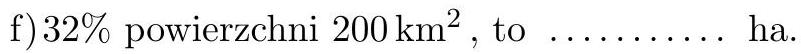
\includegraphics[max width=\textwidth, center]{2024_11_21_8f01584889ff06348ae7g-129}

\subsection*{7.3 Wyznaczanie liczby z procentu}
\section*{PRZYKŁAD}
Jaka to liczba, której \(15 \%\) równe jest 6? Innymi słowy, jakie jest rozwiązanie równania \(\frac{15}{100} x=6\) ? Przekształcając to równanie mamy \(x=\frac{6 \cdot 100}{15}\), czyli \(x=40\). A zatem \(15 \%\) liczby 40 równe jest 6 .\\
10. Oblicz w pamięci liczbę, której:\\
a) \(50 \%\) jest równe 12,5\\
b) \(20 \%\) jest równe 11\\
c) \(25 \%\) jest równe 9\\
d) \(200 \%\) jest równe 300\\
e) \(150 \%\) jest równe 30\\
f) \(20 \%\) jest równe 50\\
g) \(30 \%\) jest równe 60\\
h) \(5 \%\) jest równe 10\\
11. Znajdź liczbę, której:\\
a) \(15 \%\) jest równe 3,6\\
b) \(210 \%\) jest równe 336\\
c) \(3,5 \%\) jest równe 84\\
d) \(152 \%\) jest równe 53,2\\
e) \(10,5 \%\) jest równe 24,15\\
f) \(12 \%\) jest równe 30000\\
g) \(0,5 \%\) jest równe 20\\
12. Jeżeli \(115 \%\) pewnej liczby równe jest 460, to ile to jest \(75 \%\) tej liczby?

\section*{PRZYKŁAD}
Dzisiaj do szkoły przyszło tylko \(85 \%\) wszystkich uczniów, bowiem z powodu awarii metra pozostałych 63 uczniów nie dojechało do szkoły. Ilu uczniów liczy ta szkoła?

\section*{Rozwiązanie}
Oznaczmy przez \(x\) liczbę uczniów w tej szkole. Oznacza to, że

\[
\begin{aligned}
x-\frac{85}{100} x & =63 \\
\frac{15}{100} x & =63 \\
x & =63 \cdot \frac{100}{15} \\
x & =\frac{3 \cdot 21 \cdot 5 \cdot 20}{3 \cdot 5} \\
x & =20 \cdot 21=420
\end{aligned}
\]

Odpowiedź: w tej szkole jest 420 uczniów.\\
13. Wczoraj w jednej klasie było nieobecnych 3 uczniów, co oznaczało, że \(12 \%\) uczniów w tej klasie było nieobecnych. Ilu uczniów liczy ta klasa?\\
14. \(15 \%\) mieszkańców Xtowa ma oczy niebieskie. Pozostałych 544 mieszkańców ma inny kolor oczu. Ilu mieszkańców liczy Xtowo?\\
15. Aż 20000 osób, czyli \(40 \%\) wszystkich klientów pewnego biura turystycznego, było w ubiegłym roku na wycieczkach w Niemczech. Ilu klientów miało wobec tego to biuro w ubiegłym roku?\\
16. Pani Kasia otrzymała 270 zł podwyżki, co stanowi \(15 \%\) jej dotychczasowego wynagrodzenia. Ile wynosi jej nowe wynagrodzenie?

\section*{PRZYKŁAD}
Pierwszego dnia Jacek przeczytał \(66 \frac{2}{3} \%\) wszystkich stron pewnej książki. Drugiego dnia przeczytał \(85 \%\) tych wszystkich stron, które pozostały jeszcze po pierwszym dniu. Trzeciego dnia wieczorem przeczytał pozostałe 30 stron. Ile stron liczyła ta książka?

\section*{Rozwiązanie}
Oznaczmy przez \(x\) liczbę stron jakie pozostały do przeczytania po pierwszym dniu. Mamy wówczas

\[
\begin{aligned}
x-\frac{85}{100} x & =30 \\
\frac{15}{100} x & =30 \\
x & =\frac{30 \cdot 100}{15} \\
x & =\frac{15 \cdot 2 \cdot 100}{15}=200
\end{aligned}
\]

Czyli liczba stron jakie pozostały do przeczytania po pierwszym dniu wynosi 200. Oznaczmy sobie teraz przez y liczbę stron w tej książce. Mamy wówczas

\[
\begin{aligned}
y-\frac{66 \frac{2}{3}}{100} y & =200 \\
y-\frac{\frac{200}{3}}{100} y & =200 \\
y-\frac{200}{300} y & =200 \\
y-\frac{2}{3} y & =200 \\
\frac{1}{3} y & =200 \\
y & =600
\end{aligned}
\]

Odpowiedź: Ta książka liczyła 600 stron.\\
17. Pierwszego dnia gospodarz zerwał z drzewa \(40 \%\) wszystkich gruszek. Następnego dnia zerwał \(90 \%\) pozostałych gruszek. Ostatnie 12 gruszek pozostało na drzewie. Ile gruszek było pierwotnie na tym drzewie?\\
18. Podczas pierwszej jazdy samochodem zużyto \(20 \%\) benzyny znajdującej się w zbiorniku paliwa. Podczas drugiej jazdy zużyto 10\% ilości benzyny, która została w zbiorniku po pierwszej jeździe. Po tych dwóch jazdach zostało w zbiorniku 9 litrów benzyny. Ile litrów benzyny znajdowało się w zbiorniku przed pierwszą jazdą?

\subsection*{7.4 Liczba jako procent drugiej liczby}
\section*{PRZYKŁAD}
Jakim procentem liczby 20 jest liczba 5? Innymi słowy: ile setnych z 20 równe jest 5 ? Jest to zatem rozwiązanie równania \(\frac{p}{100} \cdot 20=5\). Mamy więc \(p=\frac{500}{20}\), czyli \(p=25\), a zatem 5 jest to \(25 \%\) z liczby 20 .\\
19. Jakim procentem liczby\\
a) 16 jest liczba 4\\
b) 40 jest liczba 4\\
c) 60 jest liczba 35\\
d) 120 jest liczba 30\\
e) 120 jest liczba 40\\
f) 40 jest liczba 120\\
g) 4 jest liczba 16\\
h) 5 jest liczba 5\\
20. Oblicz jaki procent masy 1500 kg stanowi masa\\
a) 50 kg\\
b) 120 kg\\
c) 100 kg\\
d) 1000 kg\\
e) 2000 kg

\section*{PRZYKŁAD}
W szkole jest 460 uczniów, przy czym 69 z nich jeździ do szkoły autobusem. Jaki procent uczniów tej szkoły dojeżdża do szkoły autobusem?

\section*{Rozwiązanie}
Niech \(x\) oznacza szukany procent. Przypomnijmy, że słowo procent oznacza: na sto. Mamy wówczas

\[
\begin{aligned}
\frac{x}{100} \cdot 460 & =69 \\
\frac{46}{10} x & =69 \quad / \cdot \frac{10}{46} \\
x & =\frac{69 \cdot 10}{46} \\
x & =\frac{3 \cdot 23 \cdot 10}{2 \cdot 23} \\
x & =\frac{30}{2}=15
\end{aligned}
\]

Odpowiedź: \(15 \%\) uczniów tej szkoły jeździ do szkoły autobusem.\\
21. W Xlandii mieszka 18000000 osób. Ubiegłej zimy 3060000 mieszkańców Xlandii chorowało na grypę. Jaki procent mieszkańców Xlandii chorował ubiegłej zimy na grypę?\\
22. Adam napisał pod koniec semestru trzy testy: z języka polskiego, z języka angielskiego i z matematyki. Z języka polskiego można było zdobyć maksymalnie 30 punktów, z angielskiego - 45 punktów, a z matematyki - 40 punktów. Adam zdobył następujące ilości punktów: z polskiego 24, z angielskiego 37, a z matematyki 31 . Ile procent punktów zdobył on w poszczególnych testach? Z którego testu wobec tego wypadł on najlepiej?\\
23. Wśród 32 uczniów pewnej klasy 24 ma oczy niebieskie, a 4 zielone. Jaki procent uczniów w tej klasie ma niebieskie oczy, a jaki procent ma oczy zielone?\\
24. W firmie pracowało pierwotnie 40 osób. 8 osób zostało zwolnionych z pracy, a 5 przeszło na emeryturę. Ile procent pracowników zostało zwolnionych z pracy, a ile procent przeszło na emeryturę? Ile procent pracowników tej firmy zachowało pracę?\\
25. Jaki procent wszystkich liczb naturalnych dwucyfrowych, stanowią liczby dwucyfrowe a) mniejsze od 50? b) podzielne przez 3? c) podzielne przez 5? d) niepodzielne przez 10?\\
26. Jaki procent wszystkich liczb naturalnych trzycyfrowych stanowią te liczby, które są palindromami tzn. te liczby, które czyta się tak samo wprost i wspak?\\
27. W pewnej szkole na przedmiocie matematyka przyjęty jest następujący system przeliczania punktów uzyskanych na pracach kontrolnych na oceny standardowe:

\begin{center}
\begin{tabular}{l|l|c}
Procent uzyskanych punktów & ocena słownie & liczbowo \\
\hline
ponad \(90 \%\) & bardzo dobry & 5 \\
ponad \(80 \%\) do \(90 \%\) & dobry+ & 4,5 \\
pow. \(70 \%\) do \(80 \%\) & dobry & 4 \\
pow. \(60 \%\) do \(70 \%\) & dostateczny+ & 3,5 \\
pow. \(50 \%\) do \(60 \%\) & dostateczny & 3 \\
pow. \(40 \%\) do \(50 \%\) & dopuszczajacy & 2 \\
\(40 \%\) i mniej & niedostateczny & 1 \\
\end{tabular}
\end{center}

Na pracy kontrolnej można było zdobyć maksymalnie 24 punkty. Adam zdobył 22 pkt, Bartek - 20 pkt, Celina - 15 pkt, Danka - 13 pkt, Ela 11 pkt. Ile procent punktów i jaką ocenę zdobyło każde z nich?\\
28. Towar brutto waży 120 kg , tara wynosi 6 kg . Jaki to jest procent wagi brutto?

Jeżeli w wodzie rozpuścimy sól, to otrzymany płyn nazywamy roztworem soli. Jeżeli w roztworze \(\frac{p}{100}\) jego wagi stanowi sól, to mówimy, że ten roztwór jest \(p \%\) - co czytamy \(p\) procentowy.

\section*{PRZYKŁAD}
Mamy \(8 \mathrm{~kg} 6 \%\) roztworu soli kuchennej. Jaka jest waga soli w tym roztworze?

\[
\begin{aligned}
\frac{6}{100} \cdot 8[\mathrm{~kg}] & =\frac{\text { Rozwiązanie }}{100}[\mathrm{~kg}]
\end{aligned}
\]

Odpowiedź: waga soli w tym roztworze jest równa \(\frac{48}{100} \mathrm{~kg}\).\\
29. Mamy \(15 \mathrm{~kg} 10 \%\) roztworu soli kuchennej. Wyznacz masę soli oraz masę wody w tym roztworze.\\
30. Zmieszaliśmy \(12 \mathrm{~kg} 5 \%\) roztworu soli z \(18 \mathrm{~kg} 10 \%\) roztworu soli. Jaka jest waga nowego roztworu? Jaka jest waga soli w tym nowym roztworze? Jaki procent wagi nowego roztworu stanowi sól?\\
31. Zmieszaliśmy \(12 \mathrm{~kg} 6 \%\) roztworu soli z \(8 \mathrm{~kg} 8 \%\) roztworu soli. Jaka jest waga soli w tej nowo powstałej mieszance? Jaki jest procent soli w nowo powstałej mieszance?\\
32. Zmieszaliśmy \(15 \mathrm{~kg} 8 \%\) roztworu soli z 10 kg wody. Jaka jest waga uzyskanej mieszanki? Jaka jest waga soli w tej nowej mieszance? Jaki procent wagi tej nowej mieszanki stanowi sól?\\
33. Zmieszano dwa roztwory soli. Jeden roztwór był \(5 \%\), a drugi \(8 \%\). Roztworu \(5 \%\) było 8 kg , zaś \(8 \%\) było 12 kg . Jaka była masa soli w roztworze \(5 \%\), a jaka była masa soli w roztworze \(8 \%\) ? Jaka była łączna waga nowego roztworu? Jaka była masa soli w tym nowym roztworze? Jaki procent masy tego nowego roztworu stanowiła sól?\\
34. Ze 150 kg roztworu soli odparowano 60 kg wody i otrzymano roztwór o zawartości \(5 \%\) soli. Jaka jest waga nowego roztworu? Jaka jest waga zawartej w nim soli? Jaki procent początkowej wagi roztworu stanowiła sól?\\
35. W świeżo zerwanych grzybach \(86 \%\) wagi stanowi woda, resztę czyli \(14 \%\) ich wagi stanowi tzw. sucha masa.\\
(a) Jaka jest waga wody w 12 kg świeżo zerwanych grzybów?\\
(b) Jaka jest waga suchej masy w 26 kg grzybów?\\
(c) Jaka jest waga wody w \(10,5 \mathrm{~kg}\) świeżych grzybów?\\
36. Mamy 15 kg świeżych grzybów, w których \(86 \%\) wagi stanowi woda. Wysuszyliśmy te grzyby tak, że teraz ich masa jest równa \(4 \frac{1}{2} \mathrm{~kg}\). Ile kilogramów wody wyparowało z tych grzybów w trakcie suszenia? Jaka jest waga suchej masy w tych grzybach. Jaki procent wagi w tych wysuszonych grzybach stanowi teraz woda?\\
37. W świeżo zerwanych ogórkach woda stanowi \(94 \%\) ich wagi. Jaka jest waga wody w 20 kg świeżo zerwanych ogórków, a jaka jest waga suchej masy (czyli tego co by pozostało gdyby całkowicie odparować z nich wodę)?\\
38. Świeżo zerwany arbuz zawierający \(90 \%\) wody ma wagę 6 kg . Jaka jest waga wody, a jaka suchej masy w tym arbuzie?\\
39. Mamy 15 kg świeżo zerwanych melonów. Zawartość wody w świeżo zerwanym melonie jest równa \(95 \%\). Jaka jest waga wody w tych melonach? Po pewnym czasie połowa wody zawartej w tych melonach wyparowała. Ile teraz ważą te melony? Jaki procent tej nowej wagi melonów stanowi waga wody w nich zawartej?\\
40. Woda stanowi \(84 \%\) masy ciała spragnionego wielbłąda. Po napiciu się wody masa wielbłąda wynosi 800 kg , a woda stanowi \(85 \%\) jego masy. Ile wody napił się wielbłąd?

\subsection*{7.5 Zmiany/różnice procentowe}
Obecnie będziemy zajmować się zmianami i różnicami procentowymi. Jest to pojęcie, które wymaga dobrego rozumienia pojęcia procentu i umiejętnego stosowania tego pojęcia w różnych kontekstach. Dlatego należy się stosować do poniższej b.ważnej uwagi:

UWAGA Twoim celem nie jest samo uzyskanie w jakikolwiek sposób poprawnej odpowiedzi w danym zadaniu tylko postępowanie w taki sposób jaki jest demonstrowany w poszczególnych przykładach.

\section*{PRZYKŁAD}
Liczbą o 7\% większą od liczby 40 jest liczba

\[
40+\frac{7}{100} \cdot 40=40+\frac{280}{100}=40+2,8=42,8
\]

Ogólnie: liczbą o \(p \%\) większą od liczby \(a\) jest liczba

\[
a+\frac{p}{100} a
\]

\begin{enumerate}
  \setcounter{enumi}{40}
  \item Wyznacz liczbę (możesz to robić w pamięci):\\
a) o \(50 \%\) większą od 60\\
b) o \(10 \%\) większą od 120\\
c) o \(25 \%\) większą od 80\\
d) o \(100 \%\) większą od 35\\
e) o \(75 \%\) większą od 28\\
f) o \(0,5 \%\) większą od 4\\
g) o \(110 \%\) większą od 35\\
h) o \(24 \%\) większą od 35\\
i) o \(7 \frac{1}{2} \%\) większą od 20\\
j) o \(15 \%\) większą od 36\\
k) o \(2,5 \%\) większą od 32\\
l) o \(3,7 \%\) większą od 30
  \item Po podwyżce ceny o \(5 \%\) książka kosztuje teraz 21 zł. Ile kosztowała ta książka przed podwyżką?
  \item W naszej klasie jest 16 chłopców, a dziewcząt jest o \(25 \%\) więcej. Ile osób jest w naszej klasie?
  \item Po zwiększeniu pewnej liczby o 56 okazało się, że otrzymaliśmy liczbę o \(14 \%\) większą od liczby wyjściowej. Jaka to była liczba?
  \item Paweł otrzymał premię za praktykę o \(30 \%\) większą od premii Jacka. Razem dostali oni 195,5 zł. Jaką premię otrzymał każdy z nich?
\end{enumerate}

\section*{PRZYKŁAD}
O ile procent liczba 50 jest większa od liczby 40? Odpowiedzią na to pytanie jest rozwiązanie poniższego równania, w którym niewiadomą jest \(p\)

\[
40+\frac{p}{100} \cdot 40=50
\]

Rozwiązując to równanie mamy

\[
\begin{aligned}
\frac{p}{100} \cdot 40 & =50-40 \\
\frac{40}{100} \cdot p & =10 \\
p & =\frac{10 \cdot 100}{40} \\
p & =25
\end{aligned}
\]

Zatem liczba 50 jest o \(25 \%\) większa od liczby 40 .\\
46. Policz o ile procent liczba:\\
a) 40 jest większa od każdej z liczb 22, 25, 35\\
b) 100 jest większa od każdej z liczb \(40,50,55,70,90\)\\
c) 120 jest większa od każdej z liczb \(30,40,60,90,100,110\)\\
d) 0,04 jest większa od każdej z liczb \(0,02, \quad 0,025, \quad 0,03, \quad 0,01\)\\
47. Wczoraj 1 funt brytyjski kosztował 5,60 zł. Dzisiaj cena 1 funta wzrosła o 28 groszy. O ile procent wzrosła od wczoraj cena 1 funta?\\
48. W hurtowni 10 kilogramów bananów kosztuje 30 zl , a na rynku 1 kg kosztuje \(4,80 \mathrm{zł}\). O ile procent są droższe banany na rynku niż w hurtowni, tzn. o ile procent drożej wypada cena 1 kg bananów na rynku niż w hurtowni?

\section*{PRZYKŁAD}
Wyznaczamy liczbę o \(15 \%\) mniejszą od liczby 80

\[
80-\frac{15}{100} \cdot 80=80-\frac{15 \cdot 4}{5}=80-3 \cdot 4=80-12=68
\]

Zatem liczbą o \(15 \%\) mniejszą od 80 jest 68.\\
Ogólnie: liczbą o \(p \%\) mniejszą od liczby \(a\) jest liczba

\[
a-\frac{p}{100} a
\]

\begin{enumerate}
  \setcounter{enumi}{48}
  \item Wyznacz liczbę:\\
a) o \(10 \%\) mniejszą od 90\\
b) o \(25 \%\) mniejszą od 20\\
c) o \(20 \%\) mniejszą od 50\\
d) o \(1 \%\) mniejszą od 200\\
e) o \(25 \%\) mniejszą od 100\\
f) o \(24 \%\) mniejszą od 45\\
g) o \(0,1 \%\) mniejszą od 250\\
h) o \(18 \%\) mniejszą od 60\\
i) o \(15 \%\) mniejszą od 200\\
j) o \(24 \%\) mniejszą od 35\\
k) o \(30 \%\) mniejszą od 60\\
l) o \(5 \frac{1}{2} \%\) mniejszą od 45
  \item W sklepie sportowym dokonano sezonowej \(15 \%\) obniżki cen. Przed obniżką materac kosztował 30 zł, piłka 8 zł, a parasol 24 zł. Jaka jest obecna cena każdego z tych towarów?
  \item Po obniżce cen o \(10 \%\) za drukarkę zapłacono \(450 \mathrm{zł}\). Ile kosztowała ta drukarka przed obniżką cen?
  \item Po zmniejszeniu pewnej liczby o 21 otrzymaliśmy liczbę o \(70 \%\) mniejszą od liczby wyjściowej. Co to była za liczba?
  \item 
\end{enumerate}

\begin{center}
\begin{tabular}{|c|c|c|}
\hline
\multirow{2}{*}{Dla liczby} & \multicolumn{2}{|c|}{wyznacz liczbę} \\
\cline { 2 - 3 }
 & większą o & mniejszą o \\
\hline
100 & \(5 \%\) & \(5 \%\) \\
\hline
12 & \(10 \%\) & \(8 \%\) \\
\hline
20 & \(20 \%\) & \(20 \%\) \\
\hline
10 & \(2 \frac{1}{2} \%\) & \(5 \frac{1}{2} \%\) \\
\hline
5 & \(88 \%\) & \(88 \%\) \\
\hline
15 & \(110 \%\) & \(95 \%\) \\
\hline
40 & \(200 \%\) & \(100 \%\) \\
\hline
\end{tabular}
\end{center}

\begin{enumerate}
  \setcounter{enumi}{53}
  \item Cenę książki zmniejszono wpierw o \(20 \%\), a po pewnym czasie jeszcze o 50 groszy. Obecnie książka kosztuje 3,50 zł. Jaka była pierwotna cena książki?
  \item Turysta w ciągu 3 dni przejechał 684 kilometry. Pierwszego dnia przejechał dwa razy więcej niż drugiego dnia, a trzeciego dnia o \(20 \%\) mniej niż drugiego. Ile kilometrów przejechał on trzeciego dnia? Wskazówka: zastanów się nad wprowadzanymi oznaczeniami!
\end{enumerate}

\section*{PRZYKŁAD}
O ile procent liczba 50 jest mniejsza od liczby 60? Odpowiedzią na to pytanie jest rozwiązanie równania o niewiadomej \(p\)

\[
60-\frac{p}{100} \cdot 60=50
\]

Rozwiązując to równanie mamy

\[
\begin{aligned}
-\frac{p}{100} \cdot 60 & =50-60 \\
\frac{p}{100} \cdot 60 & =10 \\
p & =\frac{10 \cdot 100}{60} \\
p & =16 \frac{2}{3}
\end{aligned}
\]

Zatem liczba 50 jest o \(16 \frac{2}{3} \%\) mniejsza od liczby 60.\\
56. O ile procent liczba:\\
a) 16 jest mniejsza od każdej z liczb 20, 24, 18\\
b) 70 jest mniejsza od każdej z liczb 100, 140, 120, 80 ,\\
c) 90 jest mniejsza od każdej z liczb 120, 100, 160, 95\\
d) 4 jest mniejsza od każdej z liczb 5, 6, \(5 \frac{1}{4}\)\\
57. Jedna akcja firmy BBB kosztowała wczoraj 30 zl , a dzisiaj kosztuje 28,50 zł. O ile procent staniały od wczoraj akcje tej firmy?\\
58. W klasie I a jest 24 uczniów, a w klasie I b o \(25 \%\) uczniów więcej. O ile procent mniej uczniów jest w klasie I a niż w klasie I b?\\
59. Zapisz odpowiednie równania:\\
a) Liczba o \(20 \%\) mniejsza od \(x\) jest równa 10\\
b) Liczba o \(20 \%\) większa od \(a\) jest równa \(b\)\\
c) Liczba o \(5 \%\) mniejsza od \(50 \%\) liczby \(x\) jest równa 19\\
d) Liczba 5 razy większa od \(15 \%\) liczby \(m\) wynosi 32\\
60. O ile procent liczba \(a\) jest większa od liczby \(b\) oraz o ile procent liczba \(b\) jest mniejsza od liczby \(a\).

\begin{center}
\begin{tabular}{|c|l|l|l|r|r|r|}
\hline
a & 40 & 30 & 30 & 100 & 90 & 100 \\
\hline
b & 20 & 10 & 20 & 70 & 20 & 50 \\
\hline
\end{tabular}
\end{center}

\begin{enumerate}
  \setcounter{enumi}{60}
  \item Uzupełnij, dokonując odpowiednich obliczeń:\\
a) Jeśli cenę towaru, który kosztował \(12 \mathrm{zł}\), podniesiemy o \(3 \mathrm{zł}\), to znaczy, że jego cena wzrośnie o ..... \%.\\
b) Jeśli wczoraj jedna akcja firmy Bim kosztowała \(20 \mathrm{zł}\), a dzisiaj kosztuje 19 zł, to znaczy, że jej wartość zmalała o ............ \(\%\).\\
c) Jeśli liczba członków klubu sportowego zwiększy się 2 razy, to znaczy, że zwiększyła się ona o \%.\\
d) Producent kapeluszy słomkowych zaplanował, że sprzeda latem 5000 kapeluszy, ale udało mu się sprzedać tylko 4500, czyli o \% mniej niż zaplanował.\\
e) Jeśli w klasie jest 12 chłopców i 15 dziewcząt, to znaczy, że dziewcząt jest o ..... \% więcej niż chłopców, zaś chłopców jest o .... \% mniej niż dziewcząt.
  \item W roku 1999 pewna firma wybudowała 200 mieszkań, w roku 2000 - 208 mieszkań, a w roku 2001 - 260 mieszkań.\\
a) O ile procent więcej mieszkań wybudowała ta firma w roku 2000 w porównaniu z rokiem 1999?\\
b) O ile procent więcej w roku 2001 w porównaniu z rokiem 2000?\\
c) O ile procent więcej w 2001 w porównaniu z rokiem 1999?\\
d) O ile procent mniej w roku 1999 w porównaniu z rokiem 2001?
  \item W naszej szkole jest 925 uczniów, w tym 510 dziewcząt.\\
a) O ile procent jest w naszej szkole więcej dziewcząt niż chłopców?\\
b) O ile procent jest mniej chłopców niż dziewcząt?
  \item Kilogram bananów kosztuje \(3,50 \mathrm{zł}\), kilogram śliwek - 4,00 zł, a kilogram brzoskwiń - 4,50 zł.\\
a) O ile procent brzoskwinie są droższe od śliwek, a o ile od bananów?\\
b) O ile procent śliwki są droższe od bananów, a o ile procent są tańsze od brzoskwiń?\\
c) O ile procent banany są tańsze od brzoskwiń?
  \item a) Lekcja w polskiej szkole trwa o \(12,5 \%\) dłużej niż w szkole szwedzkiej. Ile minut trwa jedna lekcja w szkole szwedzkiej?\\
b) Lekcja w amerykańskiej szkole trwa o \(6 \frac{2}{3} \%\) dłużej niż w szkole polskiej. Ile minut trwa jedna lekcja w szkole amerykańskiej?\\
c) Lekcja w polskiej szkole trwa o \(10 \%\) krócej niż w szkole brytyjskiej. Ile minut trwa lekcja w szkole brytyjskiej?
\end{enumerate}

\section*{PRZYKŁAD}
Towar kosztował pierwotnie \(200 \mathrm{zł}\). Cenę tę obniżano dwukrotnie. Za każdym razem obniżka ceny wynosiła \(20 \%\).\\
a) Jaka jest cena tego towaru po tych dwóch obniżkach?

Wyznaczamy cenę towaru po pierwszej obniżce o \(20 \%\)

\[
200-\frac{20}{100} \cdot 200=200-40=160
\]

A zatem cena towaru po pierwszej obniżce jest równa \(160 \mathrm{zł}\).\\
Wyznaczamy cenę po drugiej obniżce o \(20 \%\)

\[
160-\frac{20}{100} \cdot 160=160-32=128
\]

A zatem cena tego towaru po dwóch obniżkach ceny, za każdym razem o \(20 \%\), jest równa 128 złotych.\\
b) O ile procent cena końcowa jest mniejsza od ceny wyjściowej? Innymi słowy, o ile procent należałoby obniżyć cenę wyjściową 200 zl , tak aby po obniżce była ona równa \(128 \mathrm{zł}\) ?

\[
200-\frac{p}{100} \cdot 200=128 \quad \text { czyli } \quad p=36
\]

A zatem cenę wyjściową 200 złotych należy obniżyć o \(36 \%\), aby otrzymać cenę końcową 128 złotych lub inaczej mówiąc cena końcowa jest o \(36 \%\) mniejsza od ceny wyjściowej.\\
c) O ile procent cenę końcową 128 złotych należy podnieść, aby uzyskać cenę pierwotną 200 złotych?

\[
128+\frac{p}{100} \cdot 128=200 \quad \text { czyli } \quad p=56 \frac{1}{4}
\]

A zatem cenę końcową 128 złotych należy podnieść o \(56 \frac{1}{4} \%\), aby uzyskać cenę wyjściową 200 złotych.\\
66. Płaszcz kosztował początkowo 500 zł. Cenę jego obniżano dwukrotnie. Za pierwszym razem obniżka wynosiła \(20 \%\), a za drugim \(10 \%\).\\
a) Ile kosztuje płaszcz obecnie?\\
b) O ile procent zmniejszyła się jego cena początkowa po tych dwóch obniżkach?\\
c) O ile procent należałoby tę ostatnią cenę podnieść, aby uzyskać cenę początkową?\\
67. Pewien towar kosztuje \(150 \mathrm{zł}\). Oblicz ile będzie kosztował ten towar:\\
a) po podwyżce o \(20 \%\) i ponownej podwyżce o \(20 \%\);\\
b) po podwyżce o \(20 \%\) i obniżce o \(20 \%\);\\
c) po obniżce o \(20 \%\) i podwyżce o \(20 \%\).\\
68. Pierwotna cena butów była \(150 \mathrm{zł}\). Ich cenę dwukrotnie obniżano: pierwszym razem o 20\%, a drugim razem o 10\%. Jaka jest obecnie cena tych butów?\\
69. Pierwotna cena butów wynosiła \(100 \mathrm{zł}\). Właściciel sklepu podniósł wpierw tę cenę o \(10 \%\). Po pewnym czasie podniósł nową cenę o \(20 \%\). Jaka jest obecnie cena jednej pary butów w tym sklepie?\\
70. Cenę towaru podwyższono z \(450 \mathrm{zł}\) na \(540 \mathrm{zł}\), a po sezonie obniżono o taki sam procent. Jaki procent ceny początkowej stanowi cena po sezonie?\\
71. Cena pewnego towaru wynosiła pierwotnie \(100 \mathrm{zł}\). Cenę tę podwyższono o 10\%. Ile kosztuje ten towar po tej podwyżce? Następnie nowa cenę towaru obniżono o \(10 \%\). Ile kosztuje ten towar po tej obniżce?\\
72. Cena pewnego towaru wynosiła pierwotnie 100 zł. Cenę tę podwyższono o 10\%. O ile procent trzeba obniżyć teraz cenę towaru, aby po tej obniżce kosztował on tyle ile kosztował przed podwyżką?

\section*{UMOWA}
Na pytanie w stylu: o ile procent różni się cena \(A\) od ceny \(B\) należy odpowiadać następująco: a) Jeżeli cena \(A\) jest wyższa od ceny B, to cena \(A\) jest o p procent wyższa od ceny \(B\), b) Jeżeli cena A jest niższa od ceny B , to cena \(A\) jest o p procent niższa od ceny \(B \mathrm{c}\) ) w przypadku równych cen stwierdzamy tylko: ceny \(A\) i \(B\) sa równe.\\
73. Pewien towar kosztował początkowo 1000 zł. Cena towaru została podniesiona o 10\%. Po pewnym czasie cenę tegoż towaru podniesiono o 20\%. Później z kolei ostatnią cenę obniżono o \(30 \%\). O ile procent różni się obecna cena od ceny początkowej?\\
74. Pewien towar kosztował początkowo \(200 \mathrm{zł}\). Cenę pewnego towaru obniżono o 20\%. Po pewnym czasie dokonano operację obniżenia ceny tego towaru o \(30 \%\). O ile procent została obniżona cena wyjściowa tego towaru po tych dwóch zniżkach?\\
75. Cenę towaru podwyższano dwukrotnie: wpierw o \(20 \%\), a za drugim razem o \(25 \%\). Po tych podwyżkach towar kosztuje 75 zł. Oblicz cenę początkową oraz ustal o ile procent najnowsza cena jest wyższa od ceny początkowej tego towaru.\\
76. Pan Karol ważył przed urlopem 80 kg . Po urlopie przytył o 12,5\%. Następnie po pół roku pracy schudł o \(10 \%\). Ile on waży obecnie?\\
77. W wyborach brało udział 10000 osób. Było dwóch kandydatów na burmistrza kandydat A i kandydat B. Kandydat A zdobył \(40 \%\) wszystkich głosów, zaś kandydat B - \(60 \%\).\\
(a) O ile głosów więcej zdobył kandydat B od kandydata A?\\
(b) O ile głosów mniej zdobył kandydat A od kandydata B?\\
(c) O ile procent głosów więcej zdobył B od A ?\\
(d) O ile procent głosów mniej zdobył A od B?\\
78. Pan Kwiatkowski wydał \(4000 \mathrm{zł} \mathrm{w}\) ciągu trzech dni. Pierwszego dnia wydał \(30 \%\) kwoty, drugiego o \(600 \mathrm{zł}\) więcej. O ile procent mniej wydał trzeciego dnia niż pierwszego?

\subsection*{7.6 Punkty procentowe}
Pojęcie punktu procentowego wyjaśnimy na przykładach, pokazując jak ono funkcjonuje w dwóch różnych kontekstach.

\section*{PRZYKŁAD}
Towar kosztował początkowo 200 złotych. Cenę jego obniżano dwukrotnie: pierwszy raz o 20\%, a drugi raz o dalszych 10 punktów (procentowych), czyli o \(10 \%\), ale liczonych od ceny początkowej.\\
a) Jaka jest cena tego towaru po pierwszej obniżce?

\[
200-\frac{20}{100} \cdot 200=160
\]

A zatem cena tego towaru po pierwszej obniżce wynosi 160 złotych.\\
b) Jaka jest cena tego towaru po drugiej obniżce?

\[
160-\frac{10}{100} \cdot 200=140
\]

A zatem cena tego towary po drugiej obniżce, o 10 punktów procentowych tzn. 10 procent liczone od ceny wyjściowej, wynosi 140 złotych.\\
c) O ile procent cena końcowa jest niższa od ceny wyjściowej?

\[
200-\frac{p}{100} \cdot 200=140 \quad \text { czyli } \quad p=30
\]

A zatem cena końcowa jest o \(30 \%\) niższa od ceny wyjściowej.\\
d) O ile procent trzeba podnieść cenę końcową, aby uzyskać cenę wyjściową?

\[
140+\frac{p}{100} \cdot 140=200 \quad \text { czyli } \quad p=42 \frac{6}{7}
\]

A zatem cenę końcową 140 złotych należy podnieść o \(42 \frac{6}{7} \%\) aby osiągnąć cenę wyjściową.\\
79. Cena towaru wynosiła pierwotnie 200 złotych. Cenę tę obniżono wpierw o \(10 \%\), a po pewnym czasie obniżono ją ponownie o dalszych 5 punktów.\\
a) Ile kosztował ten towar po pierwszej, a ile po drugiej obniżce?\\
b) O ile procent jego cena początkowa jest wyższa od aktualnej ceny?\\
80. Pewien towar kosztował początkowo \(300 \mathrm{zł}\). Cenę tego towaru obniżano dwukrotnie. Wpierw o \(20 \%\), a następnie o dalsze 10 punktów. O ile procent trzeba by teraz zwiększyć cenę towaru, aby osiągnęła ona swoją początkową wartość?\\
81. Stężenie soli w wodzie morskiej w Morzu Północnym wynosi \(3,5 \%\), zaś w Morzu Czerwonym jest o 1,5 punkta wyższe. Jaka jest waga soli zawartej w 80 kilogramach wody z Morza Czerwonego? O ile procent więcej soli znajduje się w 100 kg wody z Morza Czerwonego niż w 100 kg wody z Morza Północnego?\\
82. W grudniu pensja miesięczna brutto pana Kowalskiego wynosiła \(1800 \mathrm{zł}\). Oblicz wysokość jego pensji w lipcu następnego roku w każdym z poniższych przypadków:\\
a) 1 stycznia podwyżka o \(5 \%\), a 1 lipca podwyżka o dalsze 3 punkty.\\
b) 1 stycznia podwyżka o \(5 \%\), a 1 lipca podwyżka o \(3 \%\).\\
c) 1 stycznia podwyżka o \(3 \%\), a 1 lipca podwyżka o dalsze 5 punktów.\\
d) 1 stycznia podwyżka o \(3 \%\), a 1 lipca podwyżka o \(5 \%\).\\
e) 1 lipca podwyżka o \(8 \%\)\\
83. Cenę towaru obniżano dwukrotnie: wpierw o \(20 \%\), a następnie o dalsze 10 punktów. O ile procent trzeba zwiększyć cenę towaru, aby osiągnęła ona swoją początkową wartość?

\section*{Odpowiedzi}
\begin{enumerate}
  \item a) \(\frac{21}{100}\),\\
b) \(\frac{95}{100}\),\\
c) \(\frac{120}{100}\),\\
d) 9. a) 22 ,\\
b) \(36 \quad\) c) 0,3125\\
d) 1\\
\(10 \frac{1}{2}\),\\
e) \(15 \frac{\frac{1}{3}}{100}\),\\
f) \(\frac{\frac{1}{2}}{100}\),\\
g) \(\frac{99 \frac{1}{2}}{100}\)\\
e) 40000\\
f) \(6400=64 \mathrm{~km}^{2}\)\\
12.300
  \item a) \(65 \%\)\\
b) \(120 \%\),\\
c) \(1 \frac{1}{2} \%\),\\
d) \(175 \%\),\\
e) \(62,5 \%\),\\
f) \(35 \%\),\\
g) 13.25 \(112 \%\)\\
14.640
  \item a) \(32 \frac{1}{2}, 29 \frac{1}{4}, 23 \frac{2}{5}, 1 \frac{5}{8}\)
  \item 50000\\
b) \(4, \frac{7}{4}, \frac{3}{5}, \frac{1}{5}\)\\
c) \(4, \quad 9 \frac{3}{5}, 6 \frac{2}{5}, 2 \frac{2}{15}\)
  \item 156, 364
  \item w SP 21 - 66 uczniów, a w SP 27
\end{enumerate}

\begin{itemize}
  \item 68 uczniów
\end{itemize}

\begin{enumerate}
  \setcounter{enumi}{5}
  \item w Nadlesie o 51 kobiet więcej
  \item 
  \item \(1800+270=2070\)
  \item po pierwszym dniu 120 , początkowo 200
  \item po pierwszej jeździe 10 litrów, początkowo 12,5 litra\\
7.w Polsce \(7,605 \mathrm{mln}\), we Francji\\
d) \(25 \%\), e) \(33 \frac{1}{3}\), f) \(300 \%\), g) \(400 \%\), 4,176 mln
  \item w Polsce \(4,68 \mathrm{mln}\), w Chinach h) \(100 \%\)
\end{enumerate}

6,75 mln\\
20.\\
a) \(3 \frac{1}{3} \%\),\\
b) \(8 \%\),\\
c) \(6 \frac{2}{3} \%\),\\
d) \(66 \frac{2}{3} \%\), e) \(133 \frac{1}{3} \%\)\\
21. 17\%\\
22. polski \(-80 \%\), angielski \(-82 \frac{2}{9} \%\), matematyka - 77,5\%\\
23. niebieskie \(-75 \%\), zielone \(-12,5 \%\)\\
24. \(20 \%, 12,5 \%, 67,5 \%\)\\
b) \(33 \frac{1}{3} \%\),\\
25. a) \(44 \frac{4}{9} \%\),\\
d) \(90 \%\)\\
c) \(20 \%\),\\
26. 10\%\\
27. Adam \(-91 \frac{2}{3} \%\), Bartek \(-83 \frac{1}{3} \%\), Celina \(-62 \frac{1}{2} \%\), Danka \(-54 \frac{1}{6} \%\),\\
Ela - \(45 \frac{5}{6} \%\)\\
28. 5\%\\
29. m. soli \(1,5 \mathrm{~kg}\), m. wody \(13,5 \mathrm{~kg}\)\\
30. \(30 \mathrm{~kg}, 2,4 \mathrm{~kg}, 8 \%\)\\
31. \(1,36 \mathrm{~kg}, 6,8 \%\)\\
32.4,8\%\\
33. \(0,4 \mathrm{~kg}, 0,96 \mathrm{~kg}, 20 \mathrm{~kg}, 6,8 \%\)\\
\(\mathbf{3 4 . 9 0} \mathrm{kg}, 4,5 \mathrm{~kg}, 3 \%\)\\
35. \(10,32 \mathrm{~kg}, 3,64 \mathrm{~kg}, 9,03 \mathrm{~kg}\)\\
36. \(10,5 \mathrm{~kg}, 2,1 \mathrm{~kg}, 53 \frac{1}{3} \%\)\\
\(\mathbf{3 7 .} 18,8 \mathrm{~kg}, 1,2 \mathrm{~kg}\)\\
\(\mathbf{3 8 . 5 , 4 \mathrm { kg } , 0 , 6 \mathrm { kg }}\)\\
39. \(14,25 \mathrm{~kg}, 7,875 \mathrm{~kg}, 90 \frac{1}{21} \%\)\\
40.50 kg\\
42.20\\
43.36\\
44. 400\\
45. Jacek 85 zł, Paweł 110,5 zł\\
47.5\%\\
48. 60\%\\
50. materac \(25,50 \mathrm{zl}\), piłka \(6,80 \mathrm{zl}\), parasol 20,40 zł\\
\(51.500 \mathrm{zł}\)\\
\(\mathbf{5 2 . 3 0}\)\\
54. 5 zł\\
55.144 km\\
57. \(5 \%\)\\
58. \(20 \%\)\\
59. a) \(x-\frac{20}{100} x=10\),\\
b) \(a+\frac{20}{100} a=b\),\\
c) \(\frac{50}{100} x-\frac{5}{100} \cdot \frac{50}{100} x=19\),\\
d) \(5 \cdot \frac{15}{100} m=32\)\\
60.1) \(100 \%, 50 \% 2) 200 \%, 66 \frac{2}{3} \%\)\\
3) \(50 \%, 33 \frac{1}{3} \%\) 4) \(42 \frac{6}{7} \%, 30 \%\);\\
5) \(350 \%, 77 \frac{7}{9} \%\) 6) \(100 \%, 50 \%\)\\
61. a) \(25 \%\), b) \(5 \%\), c) \(100 \%\),\\
d) \(10 \%\), e) \(25 \%\) i \(20 \%\)\\
62. a) \(4 \%\), b) \(25 \%\), c) \(30 \%\),\\
d) \(23 \frac{1}{13} \%\)\\
63. a) \(22 \frac{74}{83} \%\), b) \(18 \frac{32}{51} \%\)\\
64. a) od śliwek \(12,5 \%\), od bananów \(28 \frac{4}{7} \%\), b) od bananów \(14 \frac{2}{7} \%\), od brzoskwiń \(11 \frac{1}{9} \%\), c) \(22 \frac{2}{9} \%\)\\
65. a) 40 min , b) 48 min , c) 50 min\\
\(\mathbf{6 6 . 3 6 0} \mathrm{zł}, 28 \%, 38 \frac{8}{9} \%\)\\
67. a) \(216 \mathrm{zł}\), b) \(144 \mathrm{zł}\), c) \(144 \mathrm{zł}\)\\
68. \(108 \mathrm{zł}\)\\
69. \(132 \mathrm{zł}\)\\
70.96\%\\
\(71.99 \mathrm{zł}\)\\
\(72.9 \frac{1}{11} \%\)\\
73. o \(7,6 \%\) mniejsza\\
74.44\%\\
75. 50 zł, \(50 \%\)\\
76.81 kg\\
77. a) 2000 , b) 2000 , c) \(50 \%\),\\
d) \(33 \frac{1}{3} \%\)\\
\(78.16 \frac{2}{3} \%\)\\
79. a) \(180 \mathrm{zł}, 170 \mathrm{zł}\), b) \(17 \frac{11}{17} \%\)\\
80. \(42 \frac{6}{7} \%\)\\
\(81.42 \frac{6}{7} \%\)\\
82. a) \(1944 \mathrm{zł}\), b) \(1946,70 \mathrm{zl}\),\\
c) 1944,\\
d) 1946,70,\\
e) 1944 zt\\
83. \(42 \frac{6}{7} \%\)

\section*{Rozdział 8}
\section*{ZADANIA TEKSTOWE}
Obecnie zajmiemy się rozwiązywaniem zadań tekstowych dla rozwiązania których można użyć lub rozsądnie jest się posłużyć równaniem. Istotą rozwiązywania zadań tekstowych jest analiza zdań języka polskiego, które opisują pewną sytuację a następnie przekład tego na język wyrażeń algebraicznych, wyrażeń arytmetycznych oraz równań. Ostatnią rzeczą jest rozwiązanie równania. Rozwiązując zadania tekstowe pamiętaj, że twoim zasadniczym celem nie jest ustalenie poprawnej odpowiedzi na postawione w zadaniu pytanie, tylko nabycie umiejętności postępowania w taki sposób jak w zademonstrowanych w przykładach! W żadnym z tych zadań nie posługuj się kalkulatorem. Odpowiedzi podawaj w postaci ułamków zwykłych lub też w postaci liczb mieszanych.

\section*{PRZYKŁAD (1)}
\(15 \%\) pewnej liczby jest o 8 większe od \(11 \%\) tej liczby. Wyznacz tę liczbę.

\section*{Rozwiązanie}
Oznaczmy\\
\(x\) - szukana liczba.\\
Wówczas

\[
\frac{15}{100} x-15 \% \text { tej liczby, zaś } \frac{11}{100} x-11 \% \text { tej liczby. }
\]

Ponieważ \(15 \%\) tej liczby jest o 8 większe od jej \(11 \%\) oznacza to, że

\[
\frac{15}{100} x=\frac{11}{100} x+8
\]

Rozwiązując to równanie mamy:

\[
\begin{aligned}
\frac{15}{100} x & =\frac{11}{100} x+8 \\
\frac{15}{100} x-\frac{11}{100} x & =8 \\
\frac{4}{100} x & =8 \\
x & =\frac{8 \cdot 100}{4} \\
x & =200
\end{aligned}
\]

\begin{enumerate}
  \item \(10 \%\) pewnej liczby jest o 3 mniejsze od \(15 \%\) tej liczby. Wyznacz tę liczbę.
  \item W szkole jest \(35 \%\) dziewcząt, a chłopców jest o 144 więcej niż dziewcząt. Ilu jest uczniów w tej szkole?
  \item Od szyny metalowej odcięto \(72 \%\) jej długości. Masa pozostałej części szyny jest równa \(45,5 \mathrm{~kg}\). Jaka była masa całej szyny?
  \item Gdy ze zbiornika odlano \(37 \%\) jego zawartości, to zostało w nim 315 litrów wody. Ile litrów wody było początkowo w tym zbiorniku?
  \item Jeżeli pewną liczbę zwiększymy dwukrotnie, to otrzymamy liczbę o 7 większą od jednej czwartej liczby wyjściowej. Wyznacz tę liczbę.
  \item Orzechy włoskie po 4 miesiącach wskutek parowania wody straciły \(36 \%\) masy początkowej i obecnie ich masa wynosi 160 kilogramów. Jaka była ich masa na początku?
  \item Turysta szedł przez dwa dni. Pierwszego dnia przeszedł on \(2 / 3\) całej trasy, oznaczało to również, że przeszedł on o 7 km więcej niż drugiego dnia. Ile kilometrów przeszedł on pierwszego dnia?
  \item W naszej klasie \(3 / 7\) liczby wszystkich uczniów stanowią dziewczęta, których jest o 4 mniej niż chłopców. Ilu uczniów liczy nasza klasa?
  \item Na lekcji matematyki \(12 \%\) uczniów nie rozwiązało zadania, \(32 \%\) rozwiązało je z błędami rachunkowymi, a 14 uczniów rozwiązało zadanie poprawnie. Ilu uczniów liczy ta klasa?
  \item Pewnego roku \(1 / 3\) absolwentów szkół gimnazjalnych z pewnego województwa poszła uczyć się do technikum lub liceum, \(1 / 4\) do średnich szkół zawodowych, a 2000 uczniów do zasadniczych szkół zawodowych. Ilu było w sumie absolwentów szkół gimnazjalnych w tamtym roku w tym województwie, jeżeli wiadomo, że wszyscy podjęli naukę po ukończeniu gimnazjum?
  \item Połowa uczniów naszej klasy chodzi do szkoły pieszo, \(33 \frac{1}{3} \%\) dojeżdża autobusem, zaś pozostałych 5 osób rodzice dowożą do szkoły samochodem. Ilu uczniów liczy nasza klasa?
  \item Jedna trzecia wszystkich uczestników wycieczki wybrała się na zwiedzanie miasta, jedna czwarta wybrała się do teatru, jedna szósta zeszła do restauracji, zaś pozostałych 21 uczestników zostało w pokojach hotelowych. Ilu uczestników liczyła nasza wycieczka?
  \item Piąta część pszczelego roju siedzi na kwiatach jaśminu, a trzecia część na kwiatach hiacyntu. Na kwiaty róży pofrunęła liczba pszczół równa potrojonej różnicy wymienionych liczb pszczół. Ostatnia pszczoła z roju pozostała obok ula. Ile pszczół jest w tym roju?
  \item Mosiężny wałek został podzielony na trzy różnej wagi części. Na pierwszą z nich zużyto połowę wałka, na drugą \(2 / 3\) reszty. Masa trzeciej części była 3 kg . Jaka była masa całego wałka?
  \item W ciągu całego roku pan Celiński zarobił 22200 złotych. W ostatnich czterech miesiącach roku zarabiał on miesięcznie o 150 złotych więcej niż w pierwszych ośmiu miesiącach. Jaki był jego zarobek miesięczny w pierwszych ośmiu miesiącach roku?
  \item Obecnie Piotrek jest trzy razy młodszy od Waldka. Razem mają oni 8 lat. Za ile lat Waldek będzie dwa razy starszy od Piotrka?
  \item Ojciec ma 45 lat, a jego synowie 10 i 8 lat. Po ilu latach ojciec będzie miał tyle lat, ile obaj synowie razem?
  \item Do końca doby pozostało jeszcze \(20 \%\) tego czasu, który już upłynął od początku doby. Ile godzin upłynęło od początku doby?
  \item W czasie zebrania Rady Osiedla, w którym uczestniczyło 90 osób, zgłoszono wniosek o wybudowanie placu zabaw dla dzieci. Wszyscy uczestnicy zebrania wzięli udział w głosowaniu. W czasie liczenia głosów okazało się, że za wnioskiem były o 24 głosy więcej niż przeciw wnioskowi. W takiej sytuacji mówimy, że wniosek przeszedł 24 głosami. Ilu uczestników zebrania głosowało przeciw wnioskowi?
  \item W sejmie polskim zasiada 460 posłów. Gdy głosowano pewien wniosek w obecności wszystkich posłów, to przeszedł on 26 głosami. Ile osób głosowało przeciwko wnioskowi, jeżeli wiadomo, że nikt nie wstrzymał się od głosu.
  \item W czasie głosowania pewnej ustawy w sejmie (w którym jak już wiesz zasiada 460 posłów), w obecności wszystkich posłów, pewien wniosek\\
przeszedł 15 głosami, przy czym 23 posłów wstrzymało się od głosu. Ilu posłów głosowało przeciwko wnioskowi?
  \item W czasie głosowania pewnej ustawy w sejmie 44 posłów było nieobecnych. Z obecnych posłów 28 wstrzymało się od głosu. Głosowana ustawa przeszła 82 głosami. Ilu posłów głosowało przeciwko ustawie?
  \item Turysta przejechał 684 kilometry w ciągu trzech dni. Pierwszego dnia przejechał dwa razy więcej kilometrów niż drugiego dnia, a trzeciego dnia \(4 / 5\) tego co drugiego dnia. Ile kilometrów przejechał on trzeciego dnia? Zastanów się co oznaczyć w tym zadaniu jako wielkość niewiadoma.
\end{enumerate}

W kolejnym przykładzie oraz w kilku następnych zadaniach będziemy mieli do czynienia z sytuacją, gdzie do wyznaczenia są dwie wielkości których suma jest dana, natomiast w równaniu należy użyć tylko jednej niewiadomej.

\section*{PRZYKŁAD (2)}
Suma dwóch liczb równa jest 140. \(54 \%\) jednej z nich równe jest \(30 \%\) drugiej liczby. Wyznacz te liczby.

\section*{Rozwiązanie}
Niech\\
\(x\) - jedna z szukanych liczb\\
wówczas\\
\(140-x\) - druga z szukanych liczb (bo ich suma jest równa 140)\\
Wobec tego mamy

\[
\begin{aligned}
\frac{54}{100} x & =\frac{30}{100}(140-x) \\
\frac{54}{100} x & =\frac{30}{100} \cdot 140-\frac{30}{100} \cdot x \\
\frac{84}{100} x & =\frac{30}{100} \cdot 140 \\
84 x & =30 \cdot 140
\end{aligned}
\]

Uwaga! Równie dobrze moglibyśmy zapisać równanie

\[
\frac{54}{100}(140-x)=\frac{30}{100} \cdot x
\]

bowiem to jest to samo równanie co po lewej stronie. Sprawdź!

\[
x=\frac{30 \cdot 140}{84}=\frac{2 \cdot 3 \cdot 5 \cdot 2 \cdot 7 \cdot 2 \cdot 5}{2 \cdot 2 \cdot 3 \cdot 7}=2 \cdot 5 \cdot 5=50
\]

zaś

\[
140-x=140-50=90
\]

Zatem szukane liczby to 50 i 90.\\
24. Suma dwóch liczb jest równa 160, a przy tym \(30 \%\) jednej z tych liczb równe jest \(23 \frac{1}{3} \%\) drugiej liczby. Wyznacz te liczby.\\
25. W dwóch workach znajduje się łącznie 140 kg mąki. Jeżeli z pierwszego worka przesypiemy do drugiego \(12,5 \%\) mąki znajdującej się w pierwszym worku, to w obydwu workach będą jednakowe ilości mąki. Ile kilogramów mąki było początkowo w każdym worku?

\section*{PRZYKŁAD (3)}
Na konkursie należało odpowiedzieć na 30 pytań. Za każdą poprawną odpowiedź przyznawano 7 punktów, a za każdą błędną, względnie za brak odpowiedzi, odejmowano 12 punktów. Adam zdobył 77 punktów. Na ile pytań odpowiedział on poprawnie?

\section*{Rozwiązanie}
\(x\) - liczba poprawnych odpowiedzi,\\
\(30-x\) - liczba błędnych odpowiedzi.\\
Wobec tego\\
\(7 \cdot x\) - łączna liczba punktów za poprawne odpowiedzi\\
\(12 \cdot(30-x)\) - łączna liczba punktów za błędne odpowiedzi.\\
Wobec tego mamy bilans na ilość zdobytych punktów:

\[
\begin{aligned}
7 x-12(30-x) & =77 \\
7 x-360+12 x & =77 \\
19 x & =360+77 \\
x & =\frac{437}{19}=23
\end{aligned}
\]

Odp. Adam odpowiedział poprawnie na 23 pytania.\\
26. Uczeń miał do rozwiązania 10 zadań. Za każde bezbłędnie rozwiązane zadanie uczeń dostawał 10 punktów, natomiast za każde błędnie rozwiązane względnie nie rozwiązane zadanie, odejmowano mu 5 punktów. W sumie zdobył on 40 punktów. Ile zadań rozwiązał on bezbłędnie?\\
27. Księgarz zakupił w hurtowni pewną ilość egzemplarzy „Kuchni polskiej" oraz pewną ilość egzemplarzy „Poradnika majsterkowicza". W sumie kupił on 34 egzemplarze książek. Za 1 egzemplarz „Kuchni polskiej" płacił on \(23,50 \mathrm{zł}\), zaś za 1 egzemplarz „Poradnika majsterkowicza" 34 zł. W sumie zapłacił on za te 34 egzemplarze książek 904 zł. Ile egzemplarzy „Kuchni polskiej" zakupił ten księgarz?\\
28. W klasie jest 32 uczniów. Z testu historii średni wynik klasy wyniósł 26,25 punktu. Chłopcy mieli średni wynik 24 punkty, dziewczęta 28 punktów. Ilu chłopców było w klasie?

Przypomnijmy wpierw co oznacz zwrot: „p\% roztwór soli", który czytamy \(p\) procentowy roztwór soli. Oznacza to, że \(\frac{p}{100}\) masy tego roztworu stanowi sól, zaś resztę czyli \(\left(1-\frac{p}{100}\right)\) masy tego roztworu stanowi woda. Powiedzmy na przykład, że mamy 6 kilogramów \(12 \%\) roztworu soli. Oznacza to, że \(\frac{12}{100} \cdot 6[\mathrm{~kg}]\) jest masą soli w tym roztworze, czyli masa soli w tym roztworze jest równa \(\frac{72}{100}[\mathrm{~kg}]\). Natomiast masa wody w tym roztworze jest równa \(\frac{88}{100} \cdot 6[\mathrm{~kg}]\), czyli masa wody w tym roztworze wynosi \(5 \frac{28}{100}[\mathrm{~kg}]\).

\section*{PRZYKŁAD (4)}
W jednym naczyniu mamy 12 kilogramów \(10 \%\) roztworu soli. W drugim naczyniu mamy samą sól. Zmieszaliśmy to razem w trzecim naczyniu, uzyskując w efekcie roztwór \(15 \%\). Jaka była masa dosypanej soli?\\
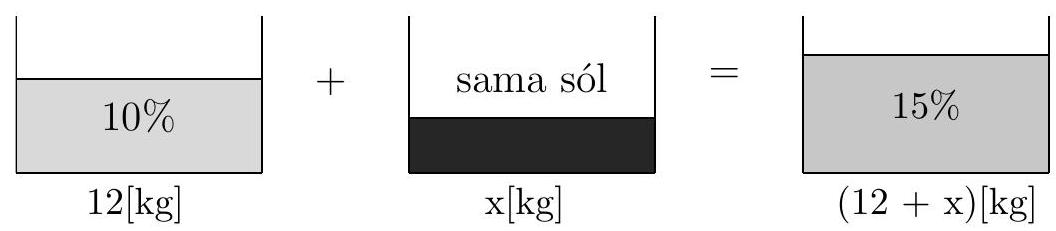
\includegraphics[max width=\textwidth, center]{2024_11_21_8f01584889ff06348ae7g-152}

Widać, że sól z pierwszego naczynia plus dosypana sól z drugiego naczynia, dają razem sól która znalazła się w trzecim naczyniu. Mamy zatem równanie na ilość soli

\[
\underbrace{\frac{10}{100} \cdot 12}_{\text {masa soli w roztw. } 10 \%}+\underbrace{x}_{\text {masa dosypanej soli }}=\underbrace{\frac{15}{100}(12+x)}_{\text {masa soli w roztw. } 15 \%}
\]

\[
\begin{aligned}
\frac{10}{100} \cdot 12+x & =\frac{15}{100} \cdot 12+\frac{15}{100} x \\
x-\frac{15}{100} x & =\frac{15}{100} \cdot 12-\frac{10}{100} \cdot 12 \\
\frac{85}{100} x & =\frac{5}{100} \cdot 12 \quad / \cdot 100 \\
85 x & =5 \cdot 12 \\
x & =\frac{5 \cdot 12}{85}=\frac{5 \cdot 12}{5 \cdot 17}=\frac{12}{17}
\end{aligned}
\]

Zatem masa soli, którą należy dosypać, aby otrzymać roztwór \(15 \%\) wynosi \(\frac{12}{17} \mathrm{~kg}\).

Innym podejściem w tym samym zadaniu jest sporządzenie bilansu (czyli równania) na ilość wody, przed i po wsypaniu soli. Zauważmy, że ilość wody w roztworze w trakcie tej operacji nie zmienia się. Przy czym\\
\(\frac{90}{100} \cdot 12[\mathrm{~kg}]\) - masa wody w roztworze \(10 \%\)\\
\(\frac{85}{100} \cdot(12+x)[\mathrm{kg}]-\) masa wody w roztworze \(15 \%\). Wobec tego mamy równanie

\[
\begin{aligned}
\underbrace{\frac{90}{100} \cdot 12}_{\text {masa wody w roztw. } 10 \%} & =\underbrace{\frac{85}{100} \cdot(12+x)}_{\text {masa wody w roztw. } 15 \%} \\
\frac{90}{100} \cdot 12 & =\frac{85}{100} 12+\frac{85}{100} x \\
\frac{90}{100} \cdot 12-\frac{85}{100} \cdot 12 & =\frac{85}{100} x \\
\frac{5}{100} \cdot 12 & =\frac{85}{100} x \\
5 \cdot 12 & =85 x \\
85 x & =5 \cdot 12 \\
x & =\frac{5 \cdot 12}{85}=\frac{5 \cdot 12}{5 \cdot 17} \\
x & =\frac{12}{17}
\end{aligned}
\]

Czyli masa soli, którą należy dosypać do \(12 \mathrm{~kg} 10 \%\) roztworu soli, aby otrzymać roztwór \(15 \%\) wynosi \(\frac{12}{17} \mathrm{~kg}\).\\
29. Do \(12 \mathrm{~kg} 15 \%\) roztworu soli dosypano pewną ilość soli i otrzymano roztwór \(20 \%\). Ile kilogramów soli dosypano?\\
30. Do \(5 \%\) roztworu soli dosypano 2 kg soli i otrzymano roztwór \(8 \%\). Jaka była masa roztworu \(5 \%\) ?\\
31. Mamy 100 kg wody morskiej o zawartości \(5 \%\) soli. Wsypano do niego pewną ilość soli i otrzymano roztwór \(7 \%\). Ile kilogramów soli wsypano?\\
32. Mamy pewną ilość \(10 \%\) roztworu soli. Po wsypaniu do niego 4 kg soli otrzymaliśmy roztwór \(12 \%\). Jaka była masa roztworu \(10 \%\) ?\\
33. W naszej szkole jest 80 uczniów, przy czym \(15 \%\) wszystkich uczniów stanowią dziewczęta. W trakcie roku szkolnego do szkoły doszła pewna liczba dziewczyn. Teraz dziewczyny stanowią \(32 \%\) liczby wszystkich uczniów? Ile dziewczyn doszło do szkoły?\\
34. W naszej szkole dziewczyny stanowią \(32 \%\) wszystkich uczniów. Gdy do szkoły doszło 75 dziewcząt, to teraz dziewczęta stanowią \(57 \frac{1}{2} \%\) liczby uczniów. Ilu uczniów liczyła pierwotnie nasza szkoła?

\section*{PRZYKŁAD (5)}
Mamy 3 kilogramy \(8 \%\) roztworu soli. Wlaliśmy do niego pewną ilość \(17 \%\) roztworu soli. Otrzymaliśmy roztwór \(11 \%\). Jaka była masa roztworu \(17 \%\). \(x\) - ilość roztworu \(17 \%\)\\
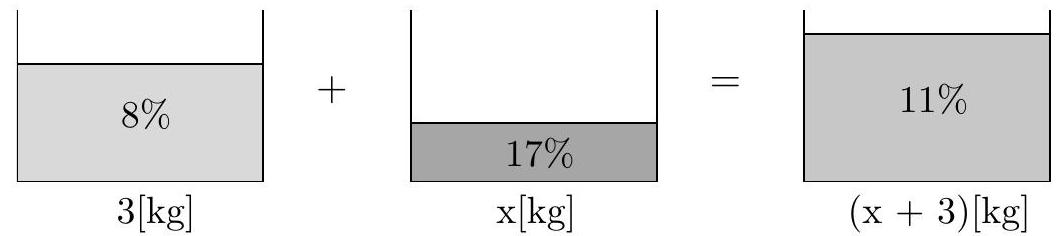
\includegraphics[max width=\textwidth, center]{2024_11_21_8f01584889ff06348ae7g-154}

Równanie na ilość soli

\[
\frac{8}{100} \cdot 3 \quad+\quad \frac{17}{100} \cdot x \quad=\quad \frac{11}{100} \cdot(x+3)
\]

I podobnie równanie na ilość wody

\[
\frac{92}{100} \cdot 3 \quad+\quad \frac{83}{100} \cdot x \quad=\quad \frac{89}{100} \cdot(x+3)
\]

Rozwiązując, na przykład, równanie na ilość wody mamy (w równaniu wyjściowym lewą i prawą stronę zamieniliśmy miejscami)

\[
\begin{aligned}
\frac{89}{100}(x+3) & =\frac{92}{100} 3+\frac{83}{100} x \\
\frac{89}{100} x+\frac{89}{100} 3 & =\frac{92}{100} 3+\frac{83}{100} x \\
\frac{89}{100} x-\frac{83}{100} x & =\frac{92}{100} 3-\frac{89}{100} 3 \\
\frac{6}{100} x & =\frac{3}{100} 3 \\
6 x & =9 \\
x & =1 \frac{1}{2}
\end{aligned}
\]

\begin{enumerate}
  \setcounter{enumi}{34}
  \item 10 kilogramów \(10 \%\) roztworu soli kuchennej zmieszano z pewną ilością \(60 \%\) roztworu soli i otrzymano roztwór \(50 \%\). Jaka była waga roztworu \(60 \%\) ?
  \item Ile kilogramów \(80 \%\) roztworu kwasu należy zmieszać z 40 kilogramami \(65 \%\) roztworu kwasu, aby otrzymać \(70 \%\) roztwór kwasu?
  \item Z naczynia wypełnionego \(96 \%\) roztworem kwasu siarkowego odlano 2,5 litra. W to miejsce wlano kwas \(80 \%\). W wyniku powstał kwas \(89 \%\). Wyznacz pojemność naczynia.
  \item Kawałek stopu miedzi z cyną ważący 12 kg zawiera \(45 \%\) miedzi. Stopiliśmy go z pewną ilością cyny. Otrzymaliśmy stop o zawartości \(40 \%\) miedzi. Ile czystej cyny dodaliśmy do stopu?
\end{enumerate}

\section*{PRZYKŁAD (6)}
Mamy \(12 \mathrm{~kg} 10 \%\) roztworu soli. Ile kilogramów wody trzeba odparować, aby otrzymać roztwór \(18 \%\) ?

\section*{Rozwiązanie}
Niech \(x[\mathrm{~kg}]\) oznacza masę wody jaką należy odparować, aby otrzymać \(18 \%\) roztwór soli.\\
Wówczas \((12-x)[\mathrm{kg}]\) oznacza masę roztworu \(18 \%\).\\
W wyniku tej operacji (odparowywania wody) masa soli w roztworze nie zmieni się.\\
Wobec tego równanie na ilość soli (przed odparowaniem wody i po odparowaniu) wygląda następująco:

\[
\begin{aligned}
\underbrace{\frac{10}{100} \cdot 12}_{\text {masa soli w roztw. } 10 \%} & =\underbrace{\frac{18}{100} \cdot(12-x)}_{\text {masa soli w roztworze } 18 \%} \\
\frac{10}{100} \cdot 12 & =\frac{18}{100} \cdot 12-\frac{18}{100} x \\
\frac{18}{100} x & =\frac{18}{100} \cdot 12-\frac{10}{100} \cdot 12 \\
\frac{18}{100} x & =\frac{8}{100} \cdot 12 \\
18 x & =8 \cdot 12 \\
x & =\frac{8 \cdot 12}{18}=5 \frac{1}{3}
\end{aligned}
\]

Czyli należy odparować \(5 \frac{1}{3} \mathrm{~kg}\) wody, aby z \(12 \mathrm{~kg} 10 \%\) roztworu soli otrzymać roztwór 18\%.\\
39. Mamy 15 kg wody morskiej o zawartości \(6 \%\) soli. Odparowaliśmy pewną ilość wody i otrzymaliśmy roztwór o zawartości \(10 \%\) soli. Jaka była waga odparowanej wody?\\
40. Mamy pewną ilość \(15 \%\) roztworu soli. Po odparowaniu 1 kg wody, otrzymaliśmy roztwór \(18 \%\). Jaka była masa roztworu \(15 \%\) ?\\
41. Z \(12 \%\) roztworu soli odparowano 4 kg wody i otrzymano roztwór \(18 \%\). Ile ważył roztwór \(12 \%\) ?\\
42. Z \(12 \mathrm{~kg} 15 \%\) roztworu soli odparowano pewną ilość wody i otrzymano roztwór \(20 \%\). Ile kilogramów wody odparowano?\\
43. 160 gramów roztworu zawierało \(1 \%\) soli, a po odparowaniu części wody otrzymano roztwór \(2 \%\). Ile waży teraz ten roztwór?\\
44. Pierwotnie w naszej szkole dziewczęta stanowiły \(40 \%\) liczby wszystkich uczniów. Ze szkoły odeszło 40 dziewczyn. Teraz dziewczyny stanowią \(32 \%\) liczby wszystkich uczniów. Ilu uczniów liczyła pierwotnie nasza szkoła?\\
45. Pierwotnie w naszej szkole dziewczęta stanowiły \(40 \%\) liczby wszystkich uczniów. Ze szkoły odeszło 40 chłopaków. Teraz dziewczyny stanowią \(48 \%\) liczby wszystkich uczniów. Ilu uczniów liczyła pierwotnie nasza szkoła?

\section*{PRZYKŁAD (7)}
Mamy \(12 \mathrm{~kg} 10 \%\) roztworu soli. Ile kilogramów wody trzeba do niego dolać, aby otrzymać roztwór \(6 \%\) ?

\section*{Rozwiązanie}
\(x[\mathrm{~kg}]\) - masa wody, którą należy dolać, aby otrzymać roztwór \(6 \%\).\\
\((12+x)[\mathrm{kg}]\) - masa roztworu \(6 \%\).\\
W wyniku tej operacji masa soli w roztworze nie zmieni się, wobec tego równanie na ilość soli wygląda następująco:

\[
\begin{aligned}
\underbrace{\frac{6}{100} \cdot(12+x)}_{\text {masa soli w roztworze } 6 \%} & =\underbrace{\frac{10}{100} \cdot 12}_{\text {masa soli w roztw. } 10 \%} \\
\frac{6}{100} \cdot 12+\frac{6}{100} \cdot x & =\frac{10}{100} \cdot 12 \\
\frac{6}{100} x & =\frac{10}{100} \cdot 12-\frac{6}{100} \cdot 12 \\
\frac{6}{100} x & =\frac{4}{100} \cdot 12 \\
6 x & =48 \\
x & =8
\end{aligned}
\]

Zatem należy dolać 8 kg wody, aby otrzymać roztwór \(6 \%\).

UWAGA W przykładach 6 i 7 można było również robić bilans na ilość wody, zamiast na ilość soli.\\
46. Do \(6 \mathrm{~kg} 8 \%\) roztworu soli dolano pewną ilość wody i otrzymano roztwór \(6 \%\). Ile wody dolano?\\
47. Do \(6 \mathrm{~kg} 12 \%\) roztworu soli dolano pewną ilość wody i w efekcie otrzymano \(10 \%\) roztwór soli. Ile wody dolano?\\
48. Mamy 45 kg wody morskiej o zawartości soli \(5 \%\). Ile wody słodkiej trzeba do niej dolać, aby otrzymać \(3 \%\) roztwór soli?\\
49. Woda morska zawiera wagowo \(5 \%\) soli. Ile kilogramów czystej wody należy dolać do 40 kg wody morskiej, aby otrzymać wodę o zawartości \(2 \%\) soli.

\section*{PRZYKŁAD (8)}
Ile kilogramów \(40 \%\), a ile \(65 \%\) roztworu soli należy wziąć, aby otrzymać 12 kg roztworu \(50 \%\) ?

\section*{Rozwiązanie}
\(x[\mathrm{~kg}]\) - masa roztworu \(40 \%\).\\
\((12-x)[\mathrm{kg}]\) - masa roztworu \(65 \%\), bo w sumie ma być ma być 12 kg . \(\frac{40}{100} x\) - masa soli w roztworze \(40 \%\)\\
\(\frac{65}{100}(12-x)\) - masa soli w roztworze \(65 \%\)\\
\(\frac{50}{100} \cdot 12\) - masa soli w uzyskanym roztworze\\
Sporządzając bilans na ilość soli mamy

\[
\begin{aligned}
\frac{40}{100} \cdot x+\frac{65}{100} \cdot(12-x) & =\frac{50}{100} \cdot 12 \\
\frac{40}{100} \cdot x+\frac{65}{100} \cdot 12-\frac{65}{100} \cdot x & =\frac{50}{100} \cdot 12 \\
-\frac{25}{100} \cdot x & =\frac{50}{100} \cdot 12-\frac{65}{100} \cdot 12 \\
-\frac{25}{100} \cdot x & =-\frac{15}{100} \cdot 12 \quad / \cdot(-100) \\
25 x & =15 \cdot 12 \\
x & =\frac{15 \cdot 12}{25}=\frac{5 \cdot 3 \cdot 12}{5 \cdot 5} \\
x & =\frac{36}{5}=7 \frac{1}{5}
\end{aligned}
\]

natomiast \(12-x\) czyli \(12-7 \frac{1}{5}\) równe jest \(4 \frac{4}{5}\). Zatem na to aby uzyskać 12 kg roztworu \(50 \%\) mając do dyspozycji roztwory \(40 \%\) i \(65 \%\) należy wziąć \(7 \frac{1}{5} \mathrm{~kg}\) roztworu \(40 \%\) oraz \(4 \frac{4}{5} \mathrm{~kg}\) roztworu \(65 \%\).\\
50. Ile kilogramów roztworu soli o stężeniu \(20 \%\) i ile kilogramów roztworu soli o stężeniu \(5 \%\) należy zmieszać ze sobą, aby otrzymać 24 kg roztworu soli o stężeniu \(10 \%\) ?\\
51. Stop zawiera \(70 \%\) miedzi, \(12 \%\) cynku, a resztę stanowi nikiel. Cynku jest o \(0,9 \mathrm{~kg}\) mniej niż niklu. Jaka była masa tego stopu? Jaka była masa cynku zawartego w tym stopie?\\
52. Stop o masie 2 kg składa się ze srebra i miedzi, przy czym masa srebra stanowi \(14 \frac{2}{7} \%\) masy miedzi. Ile waży miedź zawarta w tym stopie?\\
53. Suma trzech liczb naturalnych jest równa 210. Druga liczba stanowi \(4 / 3\) pierwszej, a trzecia liczba jest średnią arytmetyczną, czyli połową sumy, pierwszej i drugiej. Wyznacz te liczby. Zastanów się co oznaczyć jako wielkość niewiadomą.\\
54. Dane są trzy liczby, których suma jest równa 75. Pierwsza liczba stanowi 2/3 drugiej. Trzecia liczba jest średnią arytmetyczną pierwszej i drugiej. Wyznacz te liczby.\\
55. Dane są trzy liczby, których suma wynosi 36. Pierwsza liczba równa jest 3/5 trzeciej liczby. Druga liczba jest średnią arytmetyczną pierwszej i trzeciej liczby. Wyznacz te liczby.\\
56. Suma czterech liczb równa jest 19. Druga liczba jest 3 razy większa od pierwszej. Trzecia liczba jest o 5 większa od sumy dwóch pierwszych liczb. Czwarta liczba natomiast jest średnią arytmetyczną drugiej i trzeciej liczby. Wyznacz te liczby.\\
57. Mamy cztery liczby naturalne takie, że różnica pomiędzy kolejnymi wynosi 4. Iloczyn dwóch mniejszych jest o 224 mniejszy od iloczynu dwóch większych. Wyznacz te liczby.\\
58. Druga liczba jest o 3 mniejsza od pierwszej liczby. Trzecia liczba jest o 9 większa od drugiej. Średnia arytmetyczna tych trzech liczb jest równa 15. Wyznacz te liczby.\\
59. Na egzaminie \(33 \frac{1}{3} \%\) uczniów dostało oceny bdb, \(10 \%\) - dostateczne, \(\frac{1}{3}\) tych co dostali bdb - było dopuszczających, a dobrych dwa razy więcej niż dopuszczających i dostatecznych razem. Ilu było uczniów na egzaminie, jeśli 15 dostało oceny niedostateczne?\\
60. Babcia zaprosiła swoje wnuki na pierogi z jagodami. Kiedy już je przygotowała i policzyła, to okazało się, że gdyby każdemu chciała dać po 5 pierogów to zabrakłoby jej 3 pierogów, a gdyby każdemu dała po 4 pierogi, to pozostałyby jej 3 pierogi. Ile wnuków miała babcia?\\
61. Kilka osób przygotowuje wycieczkę. Jeżeli każda z nich zapłaci po 12,50 zł, to do pełnego pokrycia kosztów wycieczki zabraknie 100 zł, a jeżeli każda osoba wpłaci po \(16 \mathrm{zł}\), to po opłaceniu wszystkich kosztów zostanie \(12 \mathrm{zł}\). Ile osób bierze udział w wycieczce? Wyznacz łączny koszt tej wycieczki.\\
62. Zapytano ucznia, ile ma lat. Uczeń odpowiedział: Za 10 lat będe miat 2 razy tyle, ile miatem 4 lata temu. Ile lat ma ten uczeń?\\
63. Mój ojciec ma 3 razy więcej lat niż ja. Moi bracia mają 9 i 11 lat. Ja mam 5 razy więcej lat niż trzecia część wieku najmłodszego z braci. Za ile lat wiek ojca będzie równy sumie naszych lat?\\
64. Ojciec i córka maja razem 62 lata. 4 lata temu ojciec był 8 razy starszy od córki. Ile lat ma obecnie każde z nich?\\
65. 10 lat temu ojciec był 4 razy starszy od syna. Za 10 lat obaj będac mieli razem 100 lat. Ile lat ma obecnie każdy z nich?\\
66. Na płycie grobowca Diofantosa był napis: Pod tym kamieniem spoczywaja prochy Diofantosa, który umarl w glębokiej starości. Szósta część życia był on dzieckiem, przez dwunasta część - mlodzieńcem. Następnie upłynęta siódma część jego życia, zanim się ożenit. W 5 lat po ślubie urodzit mu się syn, który żył dwa razy krócej od niego. W 4 lata po jego śmierci Diofantos zasnął snem wieczystym. Oblicz w jakim wieku zmarł Diofantos.\\
67. Gdy do pewnej liczby dodamy jej połowę, to otrzymana suma przekroczy liczbę 60 o tyle, o ile ta liczba jest mniejsza od 65. Jaka to liczba?

W następnych kilku zadaniach możesz postępować w jeden z trzech alternatywnych sposobów:

\begin{enumerate}
  \item albo rozwiązać zadanie w pamięci (od końca), nie tworząc przy tym żadnego równania,
  \item albo wprowadzić wpierw jedną niewiadomą i rozwiązać pierwsze równanie, a potem wprowadzić drugą niewiadomą i rozwiązać drugie równanie,
  \item albo wprowadzić tylko jedną niewiadomą i rozwiązać jedno równanie.
\end{enumerate}

To pierwsze podejście jest najbardziej rozwojowe. To ostatnie podejście jest najmniej godne polecenia ze względu na zawiłość równania. Wypróbuj jednak co najmniej raz to drugie i trzecie podejście, tak aby samemu wyrobić sobie pogląd.\\
68. Sprzedawczyni sprzedała pierwszej osobie połowę wszystkich jajek i jeszcze 2 jajka. Drugiej osobie sprzedała połowę reszty jajek i jeszcze jedno jajko. Po tej drugiej sprzedaży pozostało jej 8 jajek. Ile jajek miała ona początkowo? Ile jajek kupiła pierwsza, a ile druga osoba? Zastanów się co przyjać za niewiadoma lub spróbuj rozwiazać zadanie w pamięci!\\
69. Kwiaciarka sprzedała pierwszej osobie połowę całej liczby kwiatów i jeszcze 2 kwiaty. Drugiej osobie sprzedała połowę tych kwiatów, które pozostały po pierwszej osobie i jeszcze 1 kwiat. Wtedy okazało się, ze pozostało jej tylko 5 kwiatów. Ile kwiatów kupiła pierwsza osoba?\\
70. Sprzedawca przyniósł na targ koszyk z jajkami. Pierwszej osobie sprzedał połowę wszystkich jajek i jeszcze jedno jajko, drugiej osobie połowę pozostałych jajek i jeszcze jedno jajko, trzeciej osobie połowę pozostałych jeszcze jajek i dodatkowo jedno jajko. Wówczas w koszyku pozostało 10 jajek. Ile jajek było w koszyku na początku?\\
71. Kasia rozwiązywała zadania przez trzy dni. Pierwszego dnia rozwiązała jedną trzecią wszystkich zadań i jeszcze 4 zadania. Drugiego dnia rozwiązała połowę pozostałych zadań i jeszcze 3 zadania. Trzeciego dnia rozwiązała pozostałe 17 zadań. Ile zadań rozwiązała ona łącznie w ciągu trzech dni?\\
72. Uczeń przeczytał książkę w ciągu trzech dni. Pierwszego dnia przeczytał \(25 \%\) całej książki i jeszcze 10 stron. Drugiego dnia \(\frac{5}{11}\) tego co pozostało i jeszcze 10 stron, zaś trzeciego dnia pozostałe 50 stron. Ile stron liczyła ta książka?\\
73. Ojciec rozdzielił swoje pole pomiędzy trzech synów. Najstarszemu dał \(\frac{1}{4}\) swojego pola i jeszcze 4 ha, średniemu \(\frac{1}{4}\) reszty pola i jeszcze 8 ha, a najmłodszemu \(\frac{1}{4}\) reszty oraz pozostałe 12 ha. Jaka była powierzchnia całego pola?

74* Gdyby Aleksander Wielki umarł o 5 lat wcześniej, to panowałby \(1 / 4\) swego życia, a gdyby umarł o 9 lat później, to panowałby \(1 / 2\) swego życia. Ile lat panował Aleksander Wielki?

\section*{Wskazówki i odpowiedzi.}
1.60\\
2. 480\\
3. \(162 \frac{1}{2} \mathrm{~kg}\)\\
4.500 litrów\\
5.4\\
6. 250 kg\\
7.14 km\\
8.28\\
9. 25\\
10. 4800\\
11.30\\
12.84\\
13.15\\
14.18\\
\(15.1800 \mathrm{zł}\)\\
16. za 2 lata\\
17.27\\
18. 20\\
19.33\\
20.217\\
21.211\\
22. 153\\
23.144\\
24. 70 i 90\\
25. \(80 \mathrm{~kg}, 60 \mathrm{~kg}\)\\
26.6\\
27. 24 egz.,„Kuchni pol\\
skiej", 10 egz. „Porad-\\
nika majsterkowicza"\\
28. 14 chłopców\\
29. \(0,75 \mathrm{~kg}\)\\
30. \(61 \frac{1}{3} \mathrm{~kg}\)\\
\(31.2 \frac{14}{93} \mathrm{~kg}\)\\
\(\mathbf{3 2 . 1 7 6 k g}\)\\
33. 20\\
34.125\\
35. 40 kg\\
\(\mathbf{3 6 .} 20 \mathrm{~kg}\)\\
\(37.5 \frac{5}{7}\) litra\\
38. \(1,5 \mathrm{~kg}\)\\
39.6 kg\\
40.6 kg\\
41.12 kg\\
42.3 kg\\
43.80 g\\
44.340\\
45.240\\
46.2 kg\\
\(\mathbf{4 7 . 1 , 2 k g}\)\\
48.30 kg\\
49.60 kg\\
\(\mathbf{5 0 . 8 k g ~ 2 0 \% , 1 6 k g ~ 5 \% ~}\)\\
51.15 kg - stop; \(1,8 \mathrm{~kg}\)

\begin{itemize}
  \item cynk; 10,5kg - miedź\\
\(\mathbf{5 2 . 1 , 7 5 \mathrm { kg }}\)
\end{itemize}

\begin{enumerate}
  \setcounter{enumi}{52}
  \item 60, 80, 70
  \item 20, 30, 25
  \item 9, 12, 15
  \item 1, 3, 9, 6\\
57.8; 12; 16; 20\\
58.14, 11, 20\\
59.450\\
60.6\\
61.32 osoby; \(500 \mathrm{zł}\)\\
62.18 lat\\
63.5 lat
  \item ojciec 52 lata, córka
\end{enumerate}

10 lat\\
65. ojciec 58, syn 22\\
66. 84 lata\\
67.50\\
68.40\\
69.16\\
70.94\\
71.66\\
72. 160\\
73. 48 ha\\
74. panował 12 lat, żył

33 lata

\section*{Rozdział 9}
\section*{NIERÓWNOŚCI}
\section*{PRZEDZIAŁY LICZBOWE}
Mieliśmy już do czynienia z równaniami. Obecnie będziemy mieli do czynienia z nierównościami, Te nierówności, którymi będziemy się zajmować jako rozwiązanie będą miały więcej liczb. A dokładniej mówiąc, to liczby, które będą spełniać daną nierówność będą tworzyły tzw. przedział liczbowy. Określmy wobec tego pewne przedziały liczbowe rozpoczynając od przykładów.

\section*{PRZYKŁADY}
Zbiór liczb, które spełniają nierówność \(x>2\) (co odczytujemy: \(x\) większe od 2), ma geometryczny obraz\\
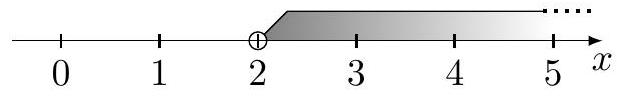
\includegraphics[max width=\textwidth, center]{2024_11_21_8f01584889ff06348ae7g-162}\\
czyli są to wszystkie liczby większe od 2 , co zapisujemy \(x \in(2,+\infty)\). Zapis \((2,+\infty)\) oznacza zbiór wszystkich liczb większych od 2.\\
Zbiór liczb, które spełniają nierówność \(x \geqslant 2\) (co odczytujemy \(x\) większe lub równe 2) ma geometryczny obraz\\
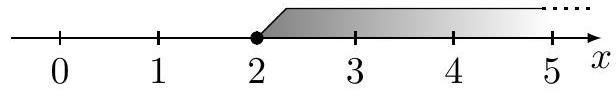
\includegraphics[max width=\textwidth, center]{2024_11_21_8f01584889ff06348ae7g-162(1)}\\
czyli są to wszystkie liczby większe lub równe 2 , co zapisujemy \(x \in[2, \infty)\). Zapis \([2, \infty)\) oznacza zbiór wszystkich liczb większych od 2 wraz z liczbą 2.

Zbiór liczb, które spełniają nierówność \(x<1\) (co odczytujemy: x mniejsze od 1) ma geometryczny obraz\\
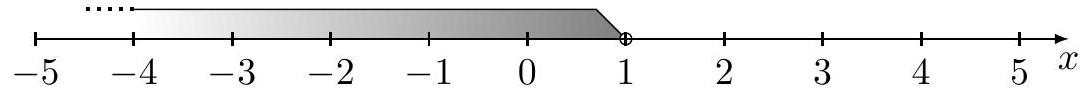
\includegraphics[max width=\textwidth, center]{2024_11_21_8f01584889ff06348ae7g-163}\\
czyli są to wszystkie liczby mniejsze od 1 , co zapisujemy \(x \in(-\infty, 1)\). Zapis \(x \in(-\infty, 1)\) oznacza zbiór wszystkich liczb mniejszych od 1.\\
Zbiór liczb, które spełniają nierówność \(x \leqslant-1\), (co odczytujemy: x mniejsze lub równe -1 ), ma geometryczny obraz\\
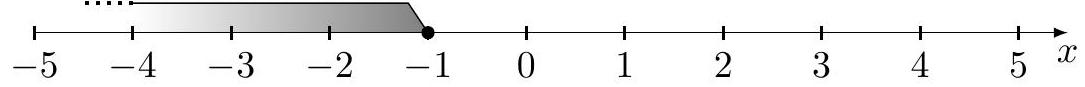
\includegraphics[max width=\textwidth, center]{2024_11_21_8f01584889ff06348ae7g-163(1)}\\
czyli są to te wszystkie liczby, które na osi liczbowej leżą na lewo od liczby -1 wraz z liczbą -1 , a co zapisujemy \(x \in(-\infty,-1]\). Zapis \(x \in(-\infty,-1]\) oznacza zbiór wszystkich liczb mniejszych od -1 wraz z liczbą -1 .\\
Ogólnie, geometrycznym obrazem zbioru liczb spełniających nierówność \(x \geqslant a\), gdzie \(a\) oznacza ustaloną liczbę, jest przedział, którego obraz na osi liczbowej jest taki jak poniżej\\
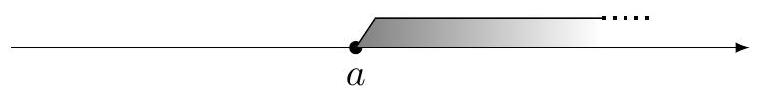
\includegraphics[max width=\textwidth, center]{2024_11_21_8f01584889ff06348ae7g-163(3)}\\
co zapisujemy \(x \in[a,+\infty)\), czyli są to te wszystkie liczby, które są większe lub równe \(a\), innymi słowami: nie mniejsze od \(a\).\\
Natomiast geometrycznym obrazem zbioru liczb spełniających nierówność \(x \leqslant a\), gdzie \(a\) oznacza ustaloną liczbę jest\\
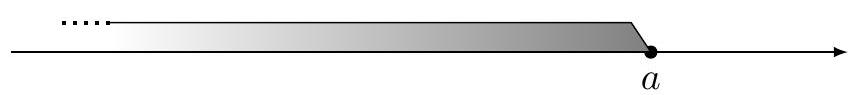
\includegraphics[max width=\textwidth, center]{2024_11_21_8f01584889ff06348ae7g-163(2)}\\
co zapisujemy \(x \in(-\infty, a]\), czyli są to te wszystkie liczby, które są mniejsze lub równe \(a\), innymi słowami, te wszystkie liczby, które są nie większe niż \(a\).

\begin{enumerate}
  \item Zaznacz na osi liczbowej zbiór tych wszystkich liczb które są\\
(a) większe od -1 ,\\
(b) nie większe od -1 ,\\
(c) większe od 1 i równocześnie mniejsze od 3 ,\\
(d) większe lub równe -1 i równocześnie mniejsze lub równe 3 .
\end{enumerate}

\section*{PRZYKŁAD .}
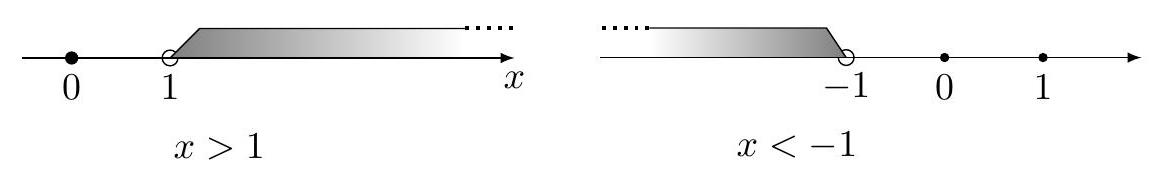
\includegraphics[max width=\textwidth, center]{2024_11_21_8f01584889ff06348ae7g-164(1)}\\
2. Na poniższych rysunkach zaznaczono zbiory liczb. Zapisz nierówność, której zbiorem rozwiązań jest zaznaczony zbiór. Następnie zaznacz i zapisz w postaci nierówności zbiór tych wszystkich liczb, które są przeciwne do liczb w zaznaczonym zbiorze.\\
\includegraphics[max width=\textwidth, center]{2024_11_21_8f01584889ff06348ae7g-164(5)}\\
a)\\
\includegraphics[max width=\textwidth, center]{2024_11_21_8f01584889ff06348ae7g-164(4)}\\
b)\\
\(\qquad\)\\
\includegraphics[max width=\textwidth, center]{2024_11_21_8f01584889ff06348ae7g-164}\\
c)\\
\includegraphics[max width=\textwidth, center]{2024_11_21_8f01584889ff06348ae7g-164(3)}\\
d)\\
\includegraphics[max width=\textwidth, center]{2024_11_21_8f01584889ff06348ae7g-164(2)}\\
e)\\
3. Zaznacz na osi liczbowej zbiór tych wszystkich liczb, dla których zbiór liczb przeciwnych ma obraz geometryczny taki jak poniżej i zapisz ten zbiór w postaci nierówności\\
\includegraphics[max width=\textwidth, center]{2024_11_21_8f01584889ff06348ae7g-165(3)}\\
a)\\
\includegraphics[max width=\textwidth, center]{2024_11_21_8f01584889ff06348ae7g-165(2)}\\
b)\\
\includegraphics[max width=\textwidth, center]{2024_11_21_8f01584889ff06348ae7g-165}\\
c)\\
\includegraphics[max width=\textwidth, center]{2024_11_21_8f01584889ff06348ae7g-165(1)}\\
d)

\section*{WNIOSKI}
Jeśli mamy \(x>a\), to \(-x<-a\)\\
Jeśli mamy \(-x<-a\), to \(x>a\)\\
Jeśli mamy \(x>-a\), to \(-x<a\)\\
Jeśli mamy \(-x \leqslant a\), to \(x \geqslant-a\)

Rozwiązywanie nierówności podobnie jak rozwiązywanie równań polega na takim ich przekształcaniu, aby każda kolejno uzyskana nierówność była równoważna poprzedzającej ją nierówności czyli, żeby miała takie samo rozwiązanie. Proces rozwiązywania kontynuujemy (zasadniczo) tak długo dopóki nie uzyskamy nierówności postaci\\
\(x<\) liczba, lub \(x \leqslant\) liczba, lub \(x>\) liczba, lub \(x \geqslant\) liczba

Z takiej postaci nierówności możemy już od razu podać zbiór tych wszystkich liczb, które spełniają tę nierówność. Zbiór tych liczb nazywamy zbiorem rozwiązań danej nierówności. Zbiory rozwiązań odpowiadające powyższym nierównościom, to kolejno

\[
(-\infty, l i c z b a), \quad(-\infty, l i c z b a], \quad(l i c z b a, \infty), \quad[l i c z b a, \infty)
\]

czyli nawias kwadratowy [ lub ] oznacza, że liczba ograniczająca przedział należy do tego przedziału, zaś nawias okrągły ( lub ) oznacza, że liczba ograniczająca nie należy do tego przedziału.\\
Przekształcanie nierówności jest technicznie podobne do przekształcania równań tzn. możemy do obu stron nierówności dodawać (odejmować) tę samą wielkość, jak również możemy obie strony nierówności mnożyć (dzielić) przez tę samą liczbę, z jedną ważną różnicą:\\
mnożąc (dzieląc) obie strony nierówności przez liczbę ujemną zamieniamy w uzyskanej nierówności znak nierówności na przeciwny!

\section*{PRZYKEAD 1}
\[
\begin{aligned}
7 x+2-(3 x-7) & \geqslant 2 x+5 \\
7 x+2-3 x+7 & \geqslant 2 x+5 \\
4 x+9 & \geqslant 2 x+5 \quad \mid-2 x,-9 \\
4 x-2 x & \geqslant 5-9 \\
2 x & \geqslant-4 \quad \mid: 2 \\
x & \geqslant-2
\end{aligned}
\]

Zatem rozwiązaniem naszej nierówności jest zbiór wszystkich liczb większych lub równych -2 czyli przedział \([-2, \infty)\)

\section*{PRZYKEAD 2}
\[
\begin{array}{rlrl}
(2 x+1)^{2}-4 x^{2} & >6 x+9 & & \\
4 x^{2}+4 x+1-4 x^{2} & >6 x+9 \\
4 x+1 & >6 x+9 \quad \text { do obu stron dodajemy }-6 x-1 \\
4 x-6 x & >9-1 \\
-2 x & >8 & & \\
x & <-4 & & \left(-\frac{1}{2}\right)
\end{array}
\]

Zatem zbiorem rozwiązań naszej nierówności jest przedział \((-\infty,-4)\), co zapisujemy \(Z R=(-\infty,-4)\)

\section*{PRZYKŁAD 3}
\[
\begin{array}{rlrl}
\frac{2 x-7}{3} & <\frac{4-5 x}{2} & \quad \mid \cdot 6 \\
2(2 x-7) & <3(4-5 x) & \\
4 x-14 & <12-15 x & & \\
4 x+15 x & <12+14 & \\
19 x & <26 & \left\lvert\, \cdot \frac{1}{19}\right. \\
x & <\frac{26}{19} &
\end{array}
\]

Zatem zbiorem rozwiązań nierówności \(\frac{2 x-7}{3}<\frac{4-5 x}{2}\) jest przedział \(\left(-\infty, \frac{26}{19}\right)\).\\
4. Rozwiąż nierówności i przedstaw zbiory rozwiązań na osi liczbowej:\\
a) \(x+\frac{1}{2} x-3<2 x\)\\
b) \(3 \geqslant(x-3)+0,5 x\)\\
c) \((x+1) x<1+\left(x^{2}+1\right)\)\\
d) \(\frac{x-3}{4} \geqslant-1\)\\
e) \(x(2 x-3)+2 x(x-2)<(2 x)^{2}+7\)\\
f) \(5 x+2 \geqslant 4(2 x-1)-3\)\\
g) \(\frac{1}{3} x>\left(4+\frac{1}{2} x\right)-2\)\\
h) \((x-3)(x+3) \leqslant(x-2)^{2}+19\)\\
i) \((x-1)^{2}>3 x+x^{2}-4\)\\
j) \(\frac{x-3}{2}<\frac{x+1}{3}\)\\
k) \((x+1) \cdot x-x^{2}<4(x-3)\)\\
l) \((x-3)^{2} \geqslant(x+2)^{2}\)\\
m) \(x+\frac{1}{2}>\frac{3 x-5}{4}\)\\
n) \((x-5) \cdot 2 \geqslant \frac{3}{2}(x-1)-1\)\\
o) \(x \leqslant \frac{2(x+1)}{3}+1-x\)\\
p) \((x-2)(x+2)>5 x-3+(x-3)^{2}\)\\
q) \(5(y-1)-5<4(y+3)+3(y-1)\)\\
r) \((3 x+2)(3 x-2)+6 x(x-1)<(3 x+4)^{2}+2 x(3 x+5)\)\\
s) \((x+3)^{2}>2 x(x+4)+9-x^{2}\)\\
5. Wyznacz zbiór rozwiązań nierówności:\\
a) \((x+2)^{2}-x^{2}>4\)\\
b) \(7 x^{2}<7(x+9)(x-9)+2 x+561\)\\
c) \((x+4)(x-4)-x^{2}<2 x\)\\
d) \(2(x-6)^{2}-2 x^{2} \geqslant 10+7 x\)\\
e) \(3(x+8)^{2}-3 x^{2} \leqslant 16+4 x\)\\
f) \((x+5)^{2} \geqslant 35+x(x-1)+12\)\\
g) \((x-5)^{2}-x^{2}<21\)\\
h) \((x-5)(x+5)>(x+3)^{2}-4\)\\
i) \((x-1)^{2}-7>x^{2}-6\)\\
j) \((x-2)(x+2)<-3 x+8+x^{2}\)\\
k) \(9 x^{2}>9(x-2)^{2}+36\)\\
l) \((x-3)^{2}>(x-1)(x+2)+4\)\\
m) \((x-1)^{2}+7 \geqslant(x+4)^{2}\)\\
n) \((1+x)^{2}+(x+3)(3-x)<14\)\\
o) \((x+2)^{2} \leqslant(x-1)^{2}+21\)\\
p) \(\frac{3(x-1)^{2}}{2}<\frac{2(x+3)^{2}}{3}+\frac{5\left(x^{2}-8 x-3\right)}{6}\)\\
q) \(\frac{(x-2)(x+2)}{2} \leqslant \frac{(x-3)^{2}}{4}+\frac{(x-1)^{2}}{4}\)\\
r) \(\frac{(x-1)^{2}}{2} \geqslant(x-1)(x+1)-\frac{(x+2)^{2}}{2}\)\\
6. Rozwiąż nierówność

\[
1+(x-3)(x+4) \leqslant(x+2)^{2}-(x+6)
\]

Podaj wszystkie liczby całkowite ujemne spełniające tę nierówność.\\
7. Rozwiąż nierówność

\[
\frac{x-3}{2}-\frac{1}{4} x<\frac{3}{4}-\frac{x+5}{2}
\]

Podaj najmniejszą liczbę całkowitą, która nie jest rozwiązaniem tej nierówności.\\
8. Rozwiąż nierówność

\[
\frac{(x-2)(2+x)}{3}+x<\frac{(x-1)^{2}+5}{3}+5
\]

Podaj największą liczbę całkowitą spełniającą tę nierówność.\\
9. Rozwiąż nierówność

\[
(x+1)^{2}-(x+2)(x-2)-3\left(x-\frac{2}{3}\right)<(x-2)^{2}-x(x-5)
\]

Jaka największa liczba całkowita nie spełnia tej nierówności?\\
10. Rozwiąż nierówność

\[
\frac{(x-1)^{2}}{2}-\frac{(x-2)^{2}}{3}-2 x<4-\frac{(1-x)(1+x)}{6}
\]

Jaka największa liczba całkowita nie spełnia tej nierówności?\\
11. Rozwiąż nierówność

\[
-3 x(x+5)+(2 x+1)^{2}+2 x>(x-3)^{2}-5 x-20
\]

Jaka najmniejsza liczba całkowita spełnia tę nierówność?

\section*{Odpowiedzi}
\begin{enumerate}
  \setcounter{enumi}{3}
  \item a) \((-6, \infty)\)\\
b) \((-\infty, 4]\)\\
c) \((-\infty, 2)\)\\
d) \([-1, \infty)\)\\
e) \((-1, \infty)\) f) \((-\infty, 3]\)\\
g) \((-\infty,-12)\)\\
h) \((-\infty, 8]\)\\
i) \((-\infty, 1)\) j) \((-\infty, 11)\)\\
k) \((4, \infty)\)\\
l) \(\left(-\infty, \frac{1}{2}\right]\)\\
m) \((-7, \infty)\)\\
n) \([15, \infty)\)\\
o) \(\left(-\infty, 1 \frac{1}{4}\right]\)\\
p) \((10, \infty)\)\\
q) \(\left.\left(-9 \frac{1}{2}, \infty\right) r\right)\)\\
\(\left(-\frac{1}{2}, \infty\right)\)\\
s) \((-\infty, 0)\)
  \item a) \((0, \infty)\)\\
b) \((3, \infty)\)\\
c) \((-8, \infty)\)\\
d) \((-\infty, 2]\)\\
e) \((-\infty,-4]\)\\
f) \([2, \infty)\)\\
g) \(\left(\frac{2}{5}, \infty\right)\)\\
h) \((-\infty,-5)\)\\
i) \((-\infty, 0)\)\\
j) \((-\infty, 4)\) k) \((2, \infty)\)\\
l) \((-\infty, 1)\)\\
m) \(\left(-\infty,-\frac{4}{5}\right]\)\\
n) \((-\infty, 2)\)\\
o) \((-\infty, 3]\)\\
p) \((-6, \infty)\)\\
q) \(\left(-\infty, 2 \frac{1}{4}\right]\)\\
r) \(\left[-3 \frac{1}{2}, \infty\right)\)
  \item \(\left[-4 \frac{1}{2}, \infty\right),-4,-3,-2,-1\)
  \item \(\left(-\infty ;-\frac{1}{3}\right) ; 0\).
  \item \((-\infty, 5) ; 4\).
  \item \(\left(1 \frac{1}{2}, \infty\right) ; 1\)
  \item \(\left(-2 \frac{4}{5} ; \infty\right) .-3\)
  \item \((-6 ; \infty),-5\)
\end{enumerate}

\section*{Rozdział 10}
\section*{UKEADY RÓWNAŃ}
Spójrzmy, na początku, na następujące zadanie:\\
2 ołówki i 2 zeszyty kosztują 8 zł.\\
2 ołówki i 3 zeszyty kosztują 10,50 zł.\\
Ile kosztuje 1 zeszyt, a ile 1 ołówek?\\
Zadanie to zapewne potrafisz rozwiązać w pamięci widząc od razu, że zeszyt kosztuje \(2,50 \mathrm{zł}\). Wiedząc już to, możesz łatwo policzyć, że 2 zeszyty kosztują 5 zł lub też że 3 zeszyty kosztują 7,50 zł. Teraz z pierwszego lub drugiego zdania możesz ustalić, że 2 ołówki kosztują 3 zł, a wobec tego 1 ołówek kosztuje 1,50 zł.\\
Jeżeli cenę ołówka oznaczamy literą np. o, zaś cenę zeszytu literą z, to treść tego zadania możemy zapisać w pewien formalny sposób zwany układem równań następująco:

\[
\left\{\begin{array}{l}
2 o+2 z=8 \\
2 o+3 z=10,50
\end{array}\right.
\]

Znak \{ rozumiemy następująco: oba warunki są równocześnie spełnione. Wówczas rozwiązanie tego układu równań, które już poznaliśmy, zapisujemy częstokroć następująco:

\[
\left\{\begin{array}{l}
o=1,50 \\
z=2,50
\end{array}\right.
\]

Proces rozwiązywania tego zadania w pamięci możemy bardziej formalnie wyrazić następująco:\\
Od równania (2) odejmujemy równanie (1) i tym sposobem dostajemy \(z=2,50\). Na to aby ustalić ile jest równe \(o\) (cena ołówka) musieliśmy\\
wziąć jedno z dwóch wyjściowych równań czyli formalnie rzecz biorąc mamy następującą sytuację

\[
\left\{\begin{aligned}
z & =2,50 \\
2 o+3 z & =10,50
\end{aligned}\right.
\]

Z pierwszego równania powyżej mamy już \(z=2,50\), wobec tego \(3 z=7,50\). Wobec tego z drugiego równania wynika, że \(2 o=3\), zaś \(o=1,50\).

To wszystko oznacza, że mając układ dwóch równań, możemy od jednego równania odjąć drugie i do tak uzyskanego równania dołączyć pierwsze lub drugie równanie z wyjściowego układu.\\
Rozważmy układ równań

\[
\left\{\begin{array}{l}
3 x+2 y=7 \\
4 x-y=2
\end{array}\right.
\]

Rozwiązaniem tego układu jest taka para liczb, która spełnia jednocześnie pierwsze i drugie równanie. Pierwsze z tych równań jest spełnione np. przez parę \(x=2, y=\frac{1}{2}\). Drugie równanie spełnione jest np. przez parę \(x=1 \frac{1}{2}\), \(y=4\). Jedyna para liczb, która spełnia równocześnie obydwa równania, to para \(x=1, y=2\). Parę taką będącą rozwiązaniem układu równań zapisujemy zazwyczaj \((1,2)\), przy czym pierwsza z tych liczb odpowiada tej zmiennej, która jest wcześniejsza alfabetycznie.

\begin{enumerate}
  \item Rozwiąż w pamięci układ równań\\
a) \(\left\{\begin{array}{l}x+y=4 \\ x+2 y=6\end{array}\right.\)\\
b) \(\left\{\begin{aligned} x+3 y & =9 \\ 0 \cdot x+y & =2\end{aligned}\right.\)\\
c) \(\left\{\begin{aligned} x+4 y & =9 \\ 2 x+0 \cdot y & =2\end{aligned}\right.\)\\
d) \(\left\{\begin{aligned} 2 x+y & =6 \\ 0 \cdot x+2 y & =4\end{aligned}\right.\)\\
e) \(\left\{\begin{array}{l}2 x+y=4 \\ 4 x+y=6\end{array}\right.\)\\
f) \(\left\{\begin{array}{l}2 x+y=7 \\ 2 x+3 y=13\end{array}\right.\)\\
g) \(\left\{\begin{array}{l}2 x+7 y=5 \\ 2 x+8 y=6\end{array}\right.\)\\
h) \(\left\{\begin{array}{l}-x+4 y=6 \\ -x+5 y=5\end{array}\right.\)\\
i) \(\left\{\begin{array}{l}2 x-3 y=7 \\ 2 x-4 y=6\end{array}\right.\)
\end{enumerate}

Jedną z formalnych metod rozwiązywania układów równań jest metoda podstawiania. Istota tej metody polega na wyznaczeniu z jednego równania jednej niewiadomej (w zależności od drugiej) i wykorzystaniu tak uzyskanej zależności w drugim z rozważanych równań.

\section*{PRZYKŁAD}
Wyznaczamy \(x\) w zależności od \(y\).

\[
\begin{aligned}
& 2 x+3 y-7=0 \\
& 2 x=-3 y+7 \\
& x=-\frac{3}{2} y+\frac{7}{2} \quad \text { wyznaczyliśmy } x \text { w zależności od } y .
\end{aligned}
\]

W tym samym równaniu możemy wyznaczyć \(y\) w zależności od \(x\).

\[
\begin{aligned}
& 2 x+3 y-7=0 \\
& 3 y=-2 x+7 \\
& y=-\frac{2}{3} x+\frac{7}{3} \quad \text { wyznaczyliśmy } y \text { w zależności od } x .
\end{aligned}
\]

PRZYKŁAD rozwiązania układu równań metodą podstawiania.

\[
\left\{\begin{array}{l}
7 x+5 y=11 \\
2 x-y=8
\end{array}\right.
\]

Z równania (2) wynika, że \(y=2 x-8\). Wstawiamy to do równania (1). Mamy wówczas

\[
\begin{aligned}
& 7 x+5(2 x-8)=11 \\
& 7 x+10 x-40=11 \\
& 17 x=51 \\
& x=3
\end{aligned}
\]

A ponieważ \(y=2 x-8\), wobec tego mamy \(y=2 \cdot 3-8=-2\) czyli rozwiązaniem wyjściowego układu równań jest para liczb \((3 ;-2)\).\\
2. Rozwiąż układ równań stosując metodę podstawiania\\
a) \(\left\{\begin{aligned} x-4 y & =9 \\ 2 x+3 y & =-4\end{aligned}\right.\)\\
b) \(\left\{\begin{array}{l}2 x+y=6 \\ 3 x-4 y=9\end{array}\right.\)\\
c) \(\left\{\begin{aligned} x-y & =4 \\ 2 x-4 y & =4\end{aligned}\right.\)\\
d) \(\left\{\begin{array}{l}2 x+y=4 \\ 4 x+3 y=14\end{array}\right.\)\\
e) \(\left\{\begin{aligned} x-3 y & =-2 \\ 2 x-y & =6\end{aligned}\right.\)\\
f) \(\left\{\begin{aligned} 4 x+2 y & =-2 \\ 3 x+5 y & =-12\end{aligned}\right.\)\\
g) \(\left\{\begin{array}{l}3 x+2 y=10 \\ 2 x-3 y=-2\end{array}\right.\)\\
h) \(\left\{\begin{array}{l}2 x+3 y=1 \\ 2 x-12 y=16\end{array}\right.\)\\
i) \(\left\{\begin{array}{l}3 x+2 y=8 \\ 6 x-2 y=10\end{array}\right.\)\\
j) \(\left\{\begin{aligned} 5 x-3 y & =13 \\ 10 x+4 y & =16\end{aligned}\right.\)\\
k) \(\left\{\begin{array}{l}4 x-8 y=8 \\ 6 x+3 y=27\end{array}\right.\)\\
l) \(\left\{\begin{aligned} 10 x-5 y & =15 \\ 2 x+6 y & =10\end{aligned}\right.\)\\
m) \(\left\{\begin{array}{l}x+2 y=6 \\ x-y=3\end{array}\right.\)\\
n) \(\left\{\begin{aligned} s+3 t & =12 \\ 2 s-t & =3\end{aligned}\right.\)\\
o) \(\left\{\begin{array}{l}4 t-2 u=2 \\ 2 t+5 u=4\end{array}\right.\)\\
p) \(\left\{\begin{array}{l}2 u-5 v=6 \\ 3 u-4 v=2\end{array}\right.\)\\
q) \(\left\{\begin{array}{l}u=3 t-2 \\ u=2 t+3\end{array}\right.\)\\
r) \(\left\{\begin{aligned} t+2 u & =2 \\ 3 t-4 u & =11\end{aligned}\right.\)\\
s) \(\left\{\begin{array}{l}b-2 a=6 \\ b=3+a\end{array}\right.\)\\
t) \(\left\{\begin{array}{l}7 a-b+17=0 \\ 5 a+6 b=8\end{array}\right.\)\\
u) \(\left\{\begin{array}{l}2 s-t=5 \\ 3 s=t-6\end{array}\right.\)

Inną formalną metodą rozwiązywania układów równań jest metoda przeciwnych współczynników.\\
PRZYKŁAD.

\[
\left\{\begin{array}{l}
3 x-2 y=-8 \\
4 x+2 y=22
\end{array}\right.
\]

Wpierw zauważ, że współczynniki przy niewiadomej \(y\) są liczbami przeciwnymi: -2 i 2 . Dodając zatem stronami powyższe dwa równania dostajemy

\[
\begin{aligned}
& (3 x-2 y)+(4 x+2 y)=-8+22 \\
& 3 x+4 x-2 y+2 y=14 \\
& 7 x=14 \\
& x=2
\end{aligned}
\]

Dzięki przeciwnym współczynnikom przy niewiadomej \(y\) po dodaniu do siebie równań zmienna \(y\) została wyeliminowana z uzyskanego równania. Wyliczona wartość \(x=2\) musi spełniać obydwa równania. Wystarczy więc wstawić tę wartość do któregokolwiek z wyjściowych równań na przykład do (2). Mamy wówczas

\[
\begin{aligned}
4 \cdot 2+2 \cdot y & =22 \\
2 y & =22-8 \\
2 y & =14 \\
y & =7
\end{aligned}
\]

Zatem rozwiązaniem układu jest para liczb (2,7), przy czym pierwsza liczba w tej parze odpowiada zmiennej \(x\), a druga liczba zmiennej \(y\), dlatego bo litera \(x\) poprzedza w alfabecie literę \(y\).\\
PRZYKŁAD

\[
\left\{\begin{array}{l}
2 x-4 y=22 \\
3 x+2 y=9
\end{array}\right.
\]

Aby doprowadzić do sytuacji, w której przy niewiadomej \(y\) są przeciwne współczynniki, należy obie strony równania (2) pomnożyć przez 2. Mamy wówczas

\[
\left\{\begin{array}{l}
2 x-4 y=22 \\
6 x+4 y=18
\end{array}\right.
\]

Gdybyśmy natomiast chcieli doprowadzić do sytuacji w której przy niewiadomej \(x\) są przeciwne współczynniki musielibyśmy (na przykład) równanie (1) pomnożyć przez 3, a równanie (2) przez -2 . Mamy wówczas

\[
\left\{\begin{array}{c}
6 x-12 y=66 \\
-6 x-4 y=-18
\end{array}\right.
\]

Dodając do siebie równania mamy

\[
\begin{aligned}
(6 x-12 y)+(-6 x-4 y) & =66+(-18) \\
6 x-6 x-12 y-4 y & =66-18 \\
-16 y & =48 \\
y & =-3
\end{aligned}
\]

Podstawiając teraz tę wartość na przykład do równania (1) mamy

\[
\begin{aligned}
2 x-4 \cdot(-3) & =22 \\
2 x+12 & =22 \\
2 x & =10 \\
x & =5
\end{aligned}
\]

Czyli rozwiązaniem rozważanego układu równań jest para liczb \((5,-3)\).\\
3. Rozwiąż układ równań metodą przeciwnych współczynników.\\
a) \(\left\{\begin{aligned} 2 x-3 y & =5 \\ 4 x+3 y & =19\end{aligned}\right.\)\\
b) \(\left\{\begin{aligned} 3 x+2 y & =-3 \\ -3 x+3 y & =-12\end{aligned}\right.\)\\
c) \(\left\{\begin{array}{l}x-y=2 \\ x+y=6\end{array}\right.\)\\
d) \(\left\{\begin{array}{l}2 x+3 y=1 \\ 3 x+4 y=2\end{array}\right.\)\\
e) \(\left\{\begin{array}{l}3 x+2 y=14 \\ 2 x-3 y=5\end{array}\right.\)\\
f) \(\left\{\begin{array}{l}4 x-3 y=6 \\ 6 x-9 y=0\end{array}\right.\)\\
g) \(\left\{\begin{array}{l}7 x+3 y=15 \\ 2 x+4 y=-2\end{array}\right.\)\\
h) \(\left\{\begin{array}{l}4 x+2 y=-10 \\ 2 x+4 y=-14\end{array}\right.\)\\
i) \(\left\{\begin{aligned} 2 s-3 t & =5 \\ s-t & =1\end{aligned}\right.\)\\
j) \(\left\{\begin{array}{l}7 v+9 z=12 \\ 9 v-8 z=35\end{array}\right.\)\\
k) \(\left\{\begin{array}{l}2 a+4 b-10=0 \\ -2 a-5 b=-18\end{array}\right.\)\\
l) \(\left\{\begin{array}{l}2 x_{1}+3 x_{2}=1 \\ 3 x_{1}+4 x_{2}=0\end{array}\right.\)\\
4. Rozwiąż układ równań\\
a) \(\left\{\begin{array}{l}(x+5)(y-2)=(x+2)(y-1) \\ (x-4)(y+7)=(x-3)(y+4)\end{array}\right.\)\\
b) \(\left\{\begin{array}{l}2(x+y)-3(x-y)=4 \\ 5(x+y)-7(x-y)=2\end{array}\right.\)\\
c) \(\left\{\begin{array}{l}x+y^{2}-4=-y+(2+y)^{2} \\ (x+y)^{2}-2 x y+x=x^{2}+y^{2}-y-4\end{array}\right.\)\\
d) \(\left\{\begin{array}{l}2(a+b)-3(a-b)=4 \\ 4(a+b)-7(a-b)=4\end{array}\right.\)\\
e) \(\left\{\begin{array}{l}2(x+1)-3(y+2)=-3 \\ x+2 y-(2 x-y)=1\end{array}\right.\)\\
f) \(\left\{\begin{array}{l}4(a+2)=1-5 b \\ 3(b+2)=3-2 a\end{array}\right.\)\\
g) \(\left\{\begin{array}{l}2 x+(2-y)^{2}+y=6+y^{2} \\ (x+y)(x-1)-2(y-2)(x+3)=x(x-y)\end{array}\right.\)\\
h) \(\left\{\begin{array}{l}2 x+y-3(x-y)=4 \\ 4(x+y)-7 x-y=-6\end{array}\right.\)\\
i) \(\left\{\begin{array}{l}(x+y)(x-y)=(x+1)^{2}-(y+2)^{2} \\ x-y=1\end{array}\right.\)\\
j) \(\left\{\begin{array}{l}2(x+1)-3(y+2)=-3 \\ x+2 y-(2 x-y)=1\end{array}\right.\)

Obecnie będziemy zajmowali się zadaniami tekstowymi, w których odpowiedź względnie łatwo uzyskuje się wprowadzając dwie niewiadome, a następnie tworząc odpowiedni układ dwóch równań i rozwiązując go. Część z poniższych zadań można by równie dobrze rozwiązać tworząc tylko jedno równanie z jedną niewiadomą, a część można rozwiązać w pamięci.

\section*{PRZYKŁAD}
Suma dwóch liczb wynosi 132. \(40 \%\) jednej z nich równe jest \(33 \frac{1}{3} \%\) drugiej. Wyznacz te liczby.\\
Oznaczenia:\\
\(x\) - jedna z szukanych liczb,\\
\(y\)-druga z szukanych liczb.\\
Mamy wówczas:

\[
\begin{array}{ll} 
\begin{cases}x+y=132 \\
\frac{40}{100} x=\frac{33 \frac{1}{3}}{100} y\end{cases} & \begin{cases}y & =132-x \\
\frac{2}{5} x & =\frac{100}{3} \cdot \frac{1}{100} y\end{cases} \\
\left\{\begin{array}{lll}
y=132-x \\
\frac{2}{5} x=\frac{\frac{100}{3}}{100} y
\end{array}\right. & \begin{cases}y & =132-x \\
\frac{2}{5} x & =\frac{1}{3} y\end{cases}
\end{array}
\]

Z równania (1) mamy wyliczone \(y=132-x\), wstawiając to do równania (2) mamy

\[
\begin{aligned}
& \frac{2}{5} x=\frac{1}{3}(132-x) \\
& \frac{2}{5} x=\frac{1}{3} \cdot 132-\frac{1}{3} x \\
& \frac{2}{5} x+\frac{1}{3} x=44 \\
& \frac{6}{15} x+\frac{5}{15} x=44 \\
& \frac{11}{15} x=44 \\
& x=\frac{44 \cdot 15}{11} \quad \text { czyli } \quad x=60
\end{aligned}
\]

Z warunku (1) wynika, że

\[
y=132-60 \text { czyli } y=72
\]

Odpowiedź: szukanymi liczbami są 60 i 72.\\
5. Suma dwóch liczb jest równa 24 , a przy tym \(62,5 \%\) jednej liczby równe jest \(75 \%\) drugiej liczby. Wyznacz te liczby.\\
6. Suma dwóch liczb wynosi 35. Jeśli pierwszą z nich zwiększymy o 20\%, a drugą zmniejszymy o \(20 \%\), to ich suma wzrośnie o 3 . Wyznacz te liczby.\\
7. Suma dwóch liczb jest 3,5 raza większa od ich różnicy. Pierwsza liczba jest o 2,4 większa od drugiej. Wyznacz te liczby.\\
8. Liczbę 185 rozkładamy na dwa składniki tak, aby jeden składnik był o 41 większy od \(60 \%\) drugiego składnika. Wyznacz oba składniki.\\
9. Suma dwóch liczb wynosi 155. Wyznacz te liczby, jeżeli \(50 \%\) pierwszej liczby równe jest \(1 / 3\) drugiej liczby.\\
10. Suma \(40 \%\) pierwszej liczby i \(20 \%\) drugiej liczby wynosi 220 . Różnica \(3 / 5\) pierwszej liczby i \(3 / 10\) drugiej liczby wynosi 150 . Wyznacz te liczby.\\
11. Różnica dwóch liczb równa jest 3. Jeżeli większą liczbę pomnożymy przez 5 , zaś od mniejszej odejmiemy 5 , to otrzymamy równe liczby. Wyznacz te liczby.\\
12. W obu klasach pierwszych było łącznie 57 uczniów. \(80 \%\) uczniów klasy Ia i \(75 \%\) klasy Ib brało udział w zawodach sportowych. Ilu uczniów liczyła każda z tych dwóch klas, jeżeli razem było 44 zawodników?\\
13. W klasach VIIa i VIIb jest łącznie 66 uczniów. W wycieczce szkolnej wzięło udział \(80 \%\) uczniów z klasy VIIa i \(75 \%\) uczniów z klasy VIIb, co stanowiło razem 51 uczniów. Ilu uczniów jest w klasie VIIa?

\section*{LICZBA, ZAPIS LICZBY.}
Liczba jest pojęciem abstrakcyjnym, natomiast zapis liczby nie jest takim pojęciem. Na co dzień nie czynimy rozróżnienia pomiędzy liczbą a zapisem liczby. Pisząc liczbę dwucyfrową o 2 dziesiątkach i 7 jednościach tworzymy zapis 27 , który jako wyrażenie arytmetyczne należy rozumieć \(2 \cdot 10+7\). Ogólnie

Liczbę o kolejnych cyfrach \(A, B, C, D\) będziemy oznaczać \(\overline{A B C D}\), przy czym \(A \neq 0\). Tutaj \(A\) oznacza ilość tysięcy, \(B\) - ilość setek, \(C\) - ilość dziesiątek, \(D\) - ilość jedności. Czyli zapis ten należy rozumieć następująco:

\[
A \cdot 10^{3}+B \cdot 10^{2}+C \cdot 10+D
\]

co zazwyczaj zapisujemy

\[
1000 A+100 B+10 C+D
\]

Zatem liczbie dwucyfrowej o \(x\) dziesiątkach i \(y\) jednościach odpowiada wyrażenie algebraiczne:

\[
x \cdot 10+y \quad \text { czyli krótko } \quad 10 x+y \text {. }
\]

Podobnie liczbie trzycyfrowej o \(x\) setkach, \(y\) dziesiątek i \(z\) jedności odpowiada wyrażenie

\[
100 x+10 y+z
\]

\section*{PRZYKŁAD}
Suma cyfr liczby dwucyfrowej równa jest 11. Jeżeli cyfrę dziesiątek zwiększymy o 4 , zaś cyfrę jedności zmniejszymy o 2 , to otrzymamy liczbę 2 razy większą (od liczby wyjściowej). Wyznacz tę liczbę.

\section*{Rozwiązanie.}
Oznaczmy\\
\(x\) - cyfra dziesiątek,\\
\(y\) - cyfra jedności.\\
Mamy zatem\\
\(10 x+y\) - szukana liczba\\
\(10(x+4)+y-2\) - otrzymana liczba o zmienionych cyfrach

Wobec tego mamy

\[
\begin{aligned}
& \begin{cases}x+y & =11 \\
10(x+4)+y-2 & =2(10 x+y)\end{cases} \\
& \begin{cases}y & =11-x \\
10 x+40+y-2 & =20 x+2 y\end{cases} \\
& \begin{cases}y=11-x \\
38=10 x+y\end{cases}
\end{aligned}
\]

W równaniu (2) w miejsce \(y\) wstawiamy \(11-x\), bo warunek (1) mówi, że \(y=11-x\). Mamy wówczas

\[
\begin{aligned}
38 & =10 x+11-x \\
27 & =9 x \\
x & =3
\end{aligned}
\]

Wobec tego \(y=11-3=8\). Zatem szukana liczbą jest 38 .\\
14. Liczba dwucyfrowa jest 7 razy większa od sumy cyfr tej liczby. Jeżeli od tej liczby odejmiemy 27, to otrzymamy liczbę powstałą z przestawienia jej cyfr. Co to za liczba.\\
15. Suma cyfr liczby dwucyfrowej jest 7 razy mniejsza od tej liczby. Liczba uzyskana z wyjściowej liczby poprzez zamianę kolejności cyfr jest o 18 mniejsza od poszukiwanej liczby. Wyznacz tę liczbę.\\
16. Suma cyfr liczby dwucyfrowej równa jest 12. Jeżeli do tej liczby dodamy 18, to otrzymamy liczbę utworzoną z tych samych cyfr, ale napisanych w odwrotnej kolejności. Wyznacz tę liczbę.\\
17. Różnica cyfry dziesiątek i cyfry jedności pewnej liczby dwucyfrowej równa jest 4. Gdy do tej szukanej liczby dodamy liczbę utworzoną z jej cyfr, ale zapisanych w odwrotnej kolejności, to otrzymamy 132. Wyznacz tę liczbę.\\
18. Suma cyfr liczby dwucyfrowej równa jest 6 . Jeśli przestawimy cyfry tej liczby, to otrzymamy liczbę, która stanowi \(4 / 7\) szukanej liczby. Co to jest za liczba?

\section*{PRZYKŁAD}
W pewnej liczbie trzycyfrowej ilość setek jest taka sama jak ilość jedności. Suma ilości setek, dziesiątek i jedności jest równa 11. Jeżeli w liczbie tej zamienimy miejscami setki z dziesiątkami, to otrzymamy liczbę o 450 większą od liczby wyjściowej. Wyznacz tę liczbę.

\section*{Rozwiązanie}
Przyjmijmy oznaczenia:\\
\(x\) - ilość setek oraz jedności w szukanej liczbie\\
\(y\) - ilość dziesiątek w tej liczbie.\\
Wówczas\\
\(100 x+10 y+x\) oznacza szukaną liczbę,\\
\(100 y+10 x+x\) oznacza liczbę z zamienionymi miejscami setkami i dziesiątkami.\\
Wobec tego mamy układ dwóch warunków

\[
\left\{\begin{array}{l}
100 y+10 x+x-450=100 x+10 y+x \\
x+y+x=11
\end{array}\right.
\]

Rozwiązując ten układ mamy

\[
\begin{aligned}
& \left\{\begin{array}{l}
100 y+10 x+x-100 x-10 y-x=450 \\
2 x+y=11
\end{array}\right. \\
& \left\{\begin{array}{l}
-90 x+90 y=450 \\
2 x+y=11
\end{array}\right. \\
& \left\{\begin{array}{l}
x-y=-5 \\
2 x+y=11
\end{array}\right.
\end{aligned}
\]

Dodając te dwa równania stronami mamy

\[
3 x=6 \quad \text { czyli } \quad x=2 \text {. }
\]

Z drugiego równania

\[
y=11-2 x \quad \text { mamy } \quad y=11-2 \cdot 2 \quad \text { czyli } \quad y=7
\]

Zatem szukaną liczbą jest 272.\\
19. W pewnej liczbie trzycyfrowej cyfra setek równa jest cyfrze dziesiątek. Liczba ta jest 25 razy większa od sumy cyfr tej liczby. Jeżeli w tej liczbie zamienimy miejscami cyfrę setek z cyfrą jedności, to otrzymamy liczbę o 297 większą od liczby wyjściowej. Wyznacz tę liczbę.\\
20. Jeżeli do liczby dwucyfrowej dopiszemy z prawej strony cyfrę dziesiątek, to otrzymamy liczbę o 227 większą. Dopisując zaś przed daną liczbą cyfrę jej jedności otrzymamy liczbę 21 razy większą. Wyznacz tę liczbę.\\
21. Liczba trzycyfrowa, w której cyfra dziesiątek wynosi 2 , jest mniejsza o 198 od liczby otrzymanej po przestawieniu cyfry jedności z cyfrą setek w tej liczbie. Jaka to liczba, jeżeli cyfra jedności jest trzy razy większa od cyfry setek?

\section*{PRZYKŁAD}
Dwie filie jednego dealera samochodowego planowały sprzedać w ciągu całego roku 550 samochodów, a faktycznie sprzedały 600 samochodów. Pierwsza filia sprzedała o \(10 \%\) więcej niż planowała, a druga filia o \(8 \%\) więcej. Ile samochodów planowała sprzedać pierwsza, a ile druga filia?

\section*{Rozwiązanie}
\section*{Oznaczenia:}
\(x\) - planowana liczba sprzedanych samochodów w pierwszej filii, \(y\) - planowana liczba sprzedanych samochodów w drugiej filii.\\
Wówczas\\
\(x+\frac{10}{100} x\) - faktyczna sprzedaż w pierwszej filii\\
\(y+\frac{8}{100} y\) - faktyczna sprzedaż w drugiej filii\\
Mamy wówczas

\[
\begin{aligned}
& \left\{\begin{array}{l}
x+y=550 \\
x+\frac{10}{100} x+y+\frac{8}{100} y=600
\end{array}\right. \\
& \left\{\begin{array}{l}
y=550-x \\
\frac{110}{100} x+\frac{108}{100} y=600
\end{array}\right. \\
& \left\{\begin{array}{l}
y=550-x \\
\frac{11}{10} x+\frac{27}{25} y=600
\end{array}\right.
\end{aligned}
\]

Wstawiając \(y\) z równania (1) do równania (2) i przekształcając następnie tylko równanie (2) mamy

\[
\begin{aligned}
& \frac{11}{10} x+\frac{27}{25}(550-x)=600 \\
& \frac{11}{10} x+\frac{27 \cdot 550}{25}-\frac{27}{25} x=600
\end{aligned}
\]

\[
\begin{aligned}
& \frac{55}{50} x+\frac{27 \cdot 22 \cdot 25}{25}-\frac{54}{50}=600 \\
& \frac{1}{50} x+27 \cdot 22=600 \\
& \frac{1}{50} x=600-594 \\
& \frac{1}{50} x=6 \quad \text { czyli } \quad x=300
\end{aligned}
\]

Wstawiając wyliczoną wartość \(x=300\) do równania (1) mamy \(y=550-300\) czyli \(y=250\).\\
22. Dwie fabryki planowały wyprodukować w ciągu miesiąca łącznie 500 maszyn. Faktycznie pierwsza fabryka wyprodukowała o \(10 \%\) więcej maszyn niż planowała, a druga o \(15 \%\) więcej. Łącznie zaś wykonały one 560 maszyn. Ile maszyn planowała wyprodukować pierwotnie pierwsza fabryka? Ile maszyn faktycznie wyprodukowała druga fabryka?\\
23. Dwa kawałki stopu: pierwszy o zawartości \(90 \%\) czystego złota i drugi o zawartości \(50 \%\) czystego złota stopiono z \(3,2 \mathrm{~g}\) czystego złota i otrzymano 10 g stopu o zawartości \(82 \%\) czystego złota. Jaka była masa każdego z kawałków?\\
24. Ile kilogramów roztworu soli o stężeniu \(20 \%\) i ile kilogramów roztworu soli o stężeniu \(5 \%\) należy zmieszać ze sobą, aby otrzymać 24 kg roztworu soli o stężeniu \(10 \%\) ?\\
25. Cyna lutownicza jest stopem czystej cyny i ołowiu. Mamy dwa kawałki cyny lutowniczej: jeden o zawartości \(24 \%\) cyny, a drugi o zawartości \(40 \%\) ołowiu. Stopiono te dwa kawałki cyny lutowniczej z 2 kilogramami ołowiu i otrzymano 10 kg cyny lutowniczej o zawartości \(30 \%\) czystej cyny. Ile ważył każdy z tych dwóch kawałków cyny lutowniczej?\\
26. Jeżeli do stopu złota ze srebrem dodamy 10 gram czystego złota, to będzie ono stanowiło \(70 \%\) masy stopu. A jeżeli dodamy 10 gram srebra, to stosunek masy złota do srebra będzie wynosił 3:2. Ile gramów złota, a ile srebra jest w stopie?\\
27. Pierwsza ruda zawiera \(72 \%\) żelaza, a druga \(58 \%\) żelaza. Po zmieszaniu obu rud dostaliśmy rudę o zawartości \(62 \%\) żelaza. Gdyby każdej z tych dwóch rud wziąć o 3 tony mniej, to otrzymalibyśmy rudę o zawartości 60,8\% żelaza. Ile ton każdej rudy wzięto do tej mieszaniny?\\
28. Wojtek z Anią mają razem 31 lat. 11 lat temu Wojtek był 2 razy starszy od Ani. Ile lat ma obecnie każde z nich?\\
29. Osiemnaście lat temu pan Nowak był trzy razy starszy od swojego syna. Obecnie jest on od niego dwa razy starszy. Ile lat ma obecnie ojciec, a ile syn?\\
30. Ojciec i córka mają razem 62 lata. 4 lata temu ojciec był 8 razy starszy od córki. Ile lat ma obecnie każde z nich?\\
31. 10 lat temu ojciec był 4 razy starszy od syna. Za 10 lat obaj będą mieli razem 100 lat. Ile lat ma obecnie każdy z nich?\\
32. 5 lat temu matka była 5 razy starsza od córki. Za 10 lat będzie ona 2 razy starsza od córki. Wyznacz ich wiek.\\
33. Za 16 lat ojciec będzie 2 razy starszy od syna. Zaś 4 lata temu był on 6 razy starszy od syna. Ile lat ma obecnie każdy z nich?\\
34. Gdyby Aleksander Wielki umarł o 5 lat wcześniej, to panowałby \(1 / 4\) swego życia, a gdyby umarł o 9 lat później, to panowałby \(1 / 2\) swego życia. Ile lat panował Aleksander Wielki?\\
35. W dwóch workach znajduje się 140 kg mąki. Jeżeli z pierwszego worka przesypiemy do drugiego 12,5\% mąki znajdującej się w pierwszym worku, to w obydwu workach będą jednakowe ilości mąki. Ile kilogramów mąki było początkowo w każdym worku?\\
36. Dwaj kolekcjonerzy znaczków zrobili zakład o jeden znaczek. Jeżeli pierwszy z nich wygra zakład, czyli dostanie 1 znaczek od tego drugiego, to będzie miał 3 razy tyle znaczków co ten drugi, a jeżeli natomiast przegra zakład, czyli odda 1 znaczek temu drugiemu, to będzie miał 2 razy tyle znaczków co drugi. Ile znaczków miał każdy z nich początkowo?\\
37. Na konkursie należało odpowiedzieć na 30 pytań. Za każdą poprawną odpowiedź przyznawano 7 punktów, a za każdą błędną odpowiedź względnie brak odpowiedzi odejmowano 12 punktów. Na ile pytań odpowiedziała dobrze osoba, która zdobyła 77 punktów?\\
38. 150\% liczby znaczków Tomka równe jest potrojonej liczbie znaczków Marcina. Ile znaczków ma każdy z nich, jeżeli razem mają oni 360 znaczków?\\
39. Napełniono miodem 20 słoików. W większych 2,5 litrowych słoikach było o 18 litrów miodu więcej niż w mniejszych 1,5 litrowych. Ile było słoików każdego rodzaju?\\
40. W dwóch zbiornikach jest benzyna. Gdybyśmy z pierwszego zbiornika przelali \(20 \%\) jego zawartości do drugiego, to w obu zbiornikach będzie tyle samo benzyny. Gdybyśmy natomiast z drugiego przelali do pierwszego 201 , to w pierwszym zbiorniku będzie 3 razy więcej benzyny niż w drugim. Ile benzyny było w każdym zbiorniku?\\
41. Z 10 kilogramów \(30 \%\) roztworu kwasu siarkowego odlano pewną ilość roztworu, a do reszty dolano roztwór \(45 \%\) i otrzymano 12 kilogramów kwasu 40\%. Ile kilogramów kwasu odlano, a ile dolano?\\
42. Stosunek dwóch liczb wynosi 4:3, a ich różnica równa jest 24. Wyznacz te dwie liczby.\\
43. Suma pól dwóch kwadratów wynosi \(100 \mathrm{~cm}^{2}\), a stosunek ich boków jest równy \(3: 4\). Oblicz długości boków tych kwadratów.\\
44. Pewnego dnia w klasie liczba uczniów nieobecnych stanowiła \(1 / 6\) liczby uczniów obecnych. Gdy na następnej lekcji jeden z uczniów wyszedł z klasy, to okazało się, że liczba uczniów nieobecnych stanowi \(1 / 5\) liczby uczniów obecnych. Ilu uczniów liczy ta klasa?\\
45. W dwóch naczyniach znajduje się woda. Jeżeli z pierwszego naczynia przelejemy do drugiego 6 litrów, to w obu naczyniach będzie tyle samo wody. Jeśli zaś z drugiego naczynia przelejemy do pierwszego 4 litry, to w pierwszym będzie dwa razy więcej wody niż w drugim. Ile litrów wody jest w każdym z naczyń?\\
46. Jeżeli licznik i mianownik pewnego ułamka zwiększymy o 1 , to otrzymamy \(\frac{4}{5}\). Gdy zaś od licznika tego ułamka odjąć 2 , a do jego mianownika dodać dwa, to otrzymamy \(\frac{5}{11}\). Co to za ułamek?\\
47. Marek i Wacek mieli pewną ilość jabłek. Marek mówi do Wacka: Daj mi jedno jabłko, to wówczas będę mial dwa razy tyle jabtek co ty. Na to Wacek mówi: Lepiej ty mi daj jedno jabłko, to wówczas będziemy mieli takie same ilości jabłek. Ile jabłek miał każdy z chłopców?\\
48. W dawnych czasach w Europie każde państwo miało własną walutę. Na przykład w Holandii były guldeny, a we Francji były franki. W kantorze skupowano waluty - franki w cenie o 2,4 grosza większej od \(60 \%\) ceny skupu jednego guldena. Za 2 guldeny i 5 franków klient otrzymał 6,92 zł. Jaka była wtedy cena skupu jednego franka, a jaka jednego guldena?\\
49. Kupiono 10 kilogramów jabłek dwóch gatunków, które kosztowały w sumie 38 złotych. Jeden gatunek kosztował \(3 \mathrm{zl} / \mathrm{kg}\), a drugi gatunek \(5 \mathrm{zl} / \mathrm{kg}\). Ile było kilogramów jabłek jednego, a ile drugiego gatunku?\\
50. Suma dwóch liczb jest 2 razy większa od ich różnicy, przy czym pierwsza liczba jest o 2,6 mniejsza od drugiej.

\section*{Odpowiedzi}
\begin{enumerate}
  \item a) \((2 ; 2)\) b) \((3 ; 2)\) 5. \(13 \frac{1}{11}, 10 \frac{10}{11}\) córka - 10 lat\\
c) \((1 ; 2)\) d) \((2 ; 2)\)\\
e) \((1 ; 2)\) f) \((2 ; 3)\)\\
g) \((-1 ; 1)\) h) \((-10 ;-1)\)\\
i) \((5 ; 1)\)
  \item a) \((1 ;-2) \quad\) b) \((3 ; 0)\)\\
c) \((6 ; 2)\) d) \((-1 ; 6)\)\\
e) \((4 ; 2)\) f) \((1 ;-3)\)\\
g) \((2 ; 2) \mathrm{h})(2 ;-1)\)\\
i) \((2 ; 1)\) j) \((2 ;-1)\)\\
k) \((4 ; 1)\) l) \((2 ; 1)\)\\
m) \((4 ; 1)\) n) \((3 ; 3)\)\\
o) \(\left(\frac{3}{4} ; \frac{1}{2}\right)\) p) \((-2 ;-2)\)\\
r) \(\left(3 ;-\frac{1}{2}\right)\)\\
q) \((5 ; 13)\)\\
t) \((-2 ; 3)\)\\
s) \((-3 ; 0)\)\\
u) \((-11 ;-27)\)
  \item a) \((4 ; 1)\) b) \((1 ;-3)\)\\
21.123\\
c) \((4 ; 2) \quad\) d) \((2 ;-1)\)
  \item 200, 300\\
e) \((4 ; 1)\) f) \((3 ; 2)\)\\
g) \((3 ;-2)\) h) \((-1 ;-3)\)
  \item \(4 \mathrm{~g}, 2,8 \mathrm{~g}\)\\
i) \((-2 ;-3)\)\\
j) \((3 ;-1)\)
  \item \(8 \mathrm{~kg}-20 \%, 16 \mathrm{~kg}-5 \%\)\\
k) \((-11 ; 8)\) l) \((-4 ; 3)\)
  \item \(5 \mathrm{~kg}-24 \%, 3 \mathrm{~kg}-40 \%\)
  \item a) \((7 ; 5)\) b) \((-19 ;-3)\)
  \item \(\mathrm{zl}-60 \mathrm{~g}, \mathrm{sr}-30 \mathrm{~g}\)\\
c) \((-1 ;-3)\) d) \((6 ; 2)\)\\
27.6, 15\\
e) \((2 ; 1)\) f) \((-3 ; 1)\)\\
g) \((10 ; 6) \mathrm{h})(4 ; 2)\)\\
i) \(\left(\frac{1}{2} ;-\frac{1}{2}\right.\)\\
j) \((2 ; 1)\)
\end{enumerate}

14 lat\\
29. 72, 36\\
30. ojciec - 52 lata,\\
31. 58, 22\\
32. matka - 30 lat, córka - 10 lat\\
33.34, 9\\
34. panowal - 12 lat, żył - 33 lata\\
35. \(80 \mathrm{~kg}, 60 \mathrm{~kg}\)\\
36.17, 7\\
37. 23, 7\\
38. 240, 120\\
39.8,12\\
40. 100, 60\\
41.6 odlano, 8 dolano\\
42. 72, 96\\
43. 8, 6\\
44. 28 osób\\
45. 24, 36\\
46. 7/9\\
47. Marek-7, Wacek-5\\
48. gulden - 1,36 zł,\\
frank - 0,84 zł\\
49.6 kg jab. po \(3 \mathrm{zl} / \mathrm{kg}\),

4 kg jab. po \(5 \mathrm{zl} / \mathrm{kg}\)\\
50. większa liczba 3,9 , mniejsza 1,3

\section*{Rozdział 11}
\section*{GEOMETRIA}
Geometria jest tą częścią matematyki, która najbardziej rozwija wyobraźnię oraz umiejętność myślenia. W pierwszej klasie zajmiemy się przede wszystkim uporządkowaniem pojęć i faktów znanych ze szkoły podstawowej. Umawiamy się, że punkty będziemy oznaczali dużymi literami, a proste małymi literami.\\
Jest dla nas rzeczą oczywistą, że przez dwa punkty na płaszczyźnie przechodzi tylko jedna prosta. Prostą przechodzącą przez punkty \(A\) i \(B\) będziemy zazwyczaj oznaczać \(l_{A B}\).

\section*{OKREŚLENIE}
\begin{center}
\includegraphics[max width=\textwidth]{2024_11_21_8f01584889ff06348ae7g-185(1)}
\end{center}

Dwie proste na płaszczyźnie, które nie mają punktu wspólnego, nazywamy prostymi równoleglymi. Fakt, że prosta \(k\) jest równoległa do prostej \(l\) zapisujemy \(k \| l\).

\section*{OKREŚLENIE}
Dwie figury, które można na siebie „nałożyć" nazywamy figurami przystajqcymi. Na rysunku obok mamy dwie pary figur przystających.\\
\includegraphics[max width=\textwidth, center]{2024_11_21_8f01584889ff06348ae7g-185}

\section*{OKREŚLENIE}
Zbiór tych punktów prostej \(A B\), które leżą pomiędzy punktami \(A\) i \(B\), nazywamy odcinkiem o końcach \(A\) i \(B\). Odcinek o końcach \(A\) i \(B\) oznaczamy \(\overline{A B}\).

Dowolny punkt na prostej dzieli ją na dwie półproste. Dowolna prosta na płaszczyźnie dzieli tę płaszczyznę na dwie półpłaszczyzny.\\
\includegraphics[max width=\textwidth, center]{2024_11_21_8f01584889ff06348ae7g-186(2)}

Punkt, w którym przecinają się dwie proste, dzieli każdą z nich na dwie półproste, zaś te dwie proste dzielą płaszczyznę na cztery rozłączne części.

\section*{OKREŚLENIE}
Każdą z tych czterech części płaszczyzny wraz z dwiema ograniczającymi ją półprostymi i punktem \(A\) nazywamy katem. Punkt \(A\) nazywamy wierzchołkiem kąta, a półproste ramionami kata.\\
\includegraphics[max width=\textwidth, center]{2024_11_21_8f01584889ff06348ae7g-186(4)}

\section*{OKREŚLENIE}
Tę parę kątów, która ma tylko wspólny wierzchołek, nazywamy parą katów wierzchotkowych.

\section*{OKREŚLENIE}
\begin{center}
\includegraphics[max width=\textwidth]{2024_11_21_8f01584889ff06348ae7g-186(3)}
\end{center}

FAKT Para kątów przyległych tworzy kąt pólpetny.\\
\includegraphics[max width=\textwidth, center]{2024_11_21_8f01584889ff06348ae7g-186}

Wiemy, że kąty wierzchołkowe są przystające.

\section*{UZASADNIENIE}
Zauważ, że zarówno kąty 1 i 2 jak i kąty 3 i 2 tworzą kąt półpełny. Wobec tego kąty 1 i 3 muszą być równe.

\section*{OKREŚLENIE}
Jeżeli wszystkie cztery kąty wierzchołkowe utworzone przez dwie przecinające się proste są przystające, to mówimy, że te proste są prostopadte, a utworzone cztery kąty nazywamy kątami prostymi.

\section*{OKREŚLENIE}
Półprosta wychodząca z wierzchołka kąta dzieląca go na dwa przystające kąty, nazywa się dwusieczna kąta. Na rysunku obok kąty 1 i 2 są równe, zaś półprosta \(l\) jest dwusieczną kąta.\\
\includegraphics[max width=\textwidth, center]{2024_11_21_8f01584889ff06348ae7g-186(1)}

\begin{itemize}
  \item Tę parę kątów, która ma wspólne ramię, a pozostałe dwa ramiona tworzą jedną prostą, nazywamy para katów przyleglych.
  \item Kąt, którego dwa ramiona i wierzchołek tworzą jedną prostą nazywamy kątem półpełnym.
\end{itemize}

\section*{UWAGA}
Kąty możemy mierzyć. Jednostką stosowaną często w mierzeniu kątów jest jeden stopień, który oznaczamy \(1^{\circ}\).

\section*{OKREŚLENIE}
Jeżeli kąt prosty podzielimy przy pomocy 89 półprostych wychodzących z jego wierzchołka na 90 przystających kątów, to każdy z tak utworzonych kątów ma miarę \(1^{\circ}\).

\section*{UWAGA}
\begin{center}
\includegraphics[max width=\textwidth]{2024_11_21_8f01584889ff06348ae7g-187}
\end{center}

Kąty zapisujemy (oznaczamy) na różne sposoby. Jeden ze sposobów polega na podaniu trzech punktów na płaszczyźnie: jednym z nich jest wierzchołek kąta, a pozostałe dwa leżą na ramionach tego kąta. Na przykład zapis \(\Varangle A B C\) oznacza, że punkt \(B\) jest wierzchołkiem kąta, punkt \(A\) leży na jednym ramieniu a punkt \(C\) na drugim ramieniu kąta. Inny sposób polega na oznaczaniu kątów greckimi literami, na przykład \(\alpha, \beta, \gamma\). Miarę kąta \(A B C\) będziemy czasami oznaczali \(|\Varangle A B C|\). Na przykład \(|\Varangle A B C|=50^{\circ}\), a gdy to nie będzie prowadziło do nieporozumień, to będziemy pisali krótko \(\Varangle A B C=50^{\circ}\).

\section*{UWAGA}
Pierwszymi pięcioma literami alfabetu greckiego są

\begin{center}
\begin{tabular}{ccccc}
alfa & beta & gamma & delta & epsilon \\
\(\boldsymbol{\alpha}\) & \(\boldsymbol{\beta}\) & \(\boldsymbol{\gamma}\) & \(\boldsymbol{\delta}\) & \(\boldsymbol{\varepsilon}\) \\
\end{tabular}
\end{center}

Teraz wiesz już zapewne od czego pochodzi słowo alfabet. Innymi literami alfabetu greckiego, których będziemy używać, są

\begin{center}
\begin{tabular}{cccc}
lambda & fi & sigma & omega \\
\(\boldsymbol{\lambda}\) & \(\boldsymbol{\varphi}\) & \(\boldsymbol{\sigma}\) & \(\boldsymbol{\omega}\) \\
\end{tabular}
\end{center}

\begin{enumerate}
  \item Jeżeli kąt prosty podzielimy jedną półprostą na dwa przystające kąty, to ile stopni ma każdy z tych dwóch kątów? A jeżeli podzielimy czterema półprostymi na pięć przystających części, to ile stopni będzie miała każda z tych pięciu części?
  \item Dwie przecinające się proste podzieliły płaszczyznę na cztery części, z których każda jest kątem. Suma dwóch spośród czterech uzyskanych kątów jest równa \(49^{\circ}\). Wyznacz miary wszystkich czterech kątów uzyskanych w wyniku przecięcia się tych dwóch prostych.
  \item Wyznacz miary wszystkich kątów uzyskanych w wyniku przecięcia się dwóch prostych jeżeli trzy z nich dają w sumie \(270^{\circ}\).
  \item Wiemy, że \(\alpha\) i \(\beta\) tworzą parę kątów przyległych. Wiemy również, że\\
a) \(\alpha-\beta=30^{\circ}\)\\
b) \(\alpha=90^{\circ}+\beta\)\\
c) \(\alpha=3 \beta\)\\
d) \(\alpha: \beta=1: 5\)
\end{enumerate}

Wyznacz miary kątów \(\alpha\) i \(\beta\) w każdym z powyższych przypadków.\\
5. Jeden z kątów, który uzyskuje się przy przecięciu dwóch prostych jest o \(50^{\circ}\) mniejszy od drugiego kąta. Wyznacz ich miary.\\
6. Jeden z kątów, który uzyskuje się przy przecięciu dwóch prostych jest cztery razy większy od drugiego. Wyznacz miary tych kątów.

\section*{PRZYKŁAD}
\begin{center}
\includegraphics[max width=\textwidth]{2024_11_21_8f01584889ff06348ae7g-188}
\end{center}

Proste \(A C\) i \(B D\) na rysunku obok przecinają się w punkcie \(O\). Wiemy, że\\
\(\Varangle A O B=\frac{1}{8}(\Varangle B O C+\Varangle C O D+\Varangle D O A)\).\\
Wyznacz miarę kąta \(A O B\).\\
Oznaczmy \(|\Varangle A O B|=\alpha=|\Varangle C O D|\), bo kąty \(A O B\) i \(C O D\) są wierzchołkowe, oraz \(\quad|\Varangle B O C|=\beta=|\Varangle A O D|\), bo kąty \(B O C\) i \(A O D\) są wierzchołkowe przy czym \(\alpha+\beta=180^{\circ}\), lub też pisząc inaczej \(\beta=180^{\circ}-\alpha\), bo \(A O B\) i \(B O C\) są kątami przyległymi.\\
Wobec tego mamy

\[
\begin{aligned}
\alpha & =\frac{1}{8}(\beta+\alpha+\beta) \\
\alpha & =\frac{1}{8}\left(180^{\circ}+\beta\right), \quad \text { bo } \quad \beta+\alpha=180^{\circ} \\
\alpha & =\frac{1}{8}\left(180^{\circ}+180^{\circ}-\alpha\right), \text { bo } \quad \beta=180^{\circ}-\alpha \\
\alpha & =\frac{1}{8}\left(360^{\circ}-\alpha\right) \\
\alpha & =\frac{1}{8} \cdot 360^{\circ}-\frac{1}{8} \alpha \\
\frac{9}{8} \alpha & =45^{\circ} \\
\alpha & =\frac{8}{9} \cdot 45^{\circ} \\
\alpha & =40^{\circ}
\end{aligned}
\]

czyli \(\Varangle A O B=40^{\circ}\).\\
\includegraphics[max width=\textwidth, center]{2024_11_21_8f01584889ff06348ae7g-189}\\
7. Proste \(X Y\) i \(W Z\) na rysunku obok przecinają się w punkcie \(P\). Wiemy, że \(|\Varangle W P X|=2|\Varangle W P Y|\). Wyznacz \(|\Varangle Y P Z|\).\\
8. Odcinki \(A B\) i \(P Q\) przecinają się w punkcie \(O\) przy czym \(\Varangle P O A=\frac{2}{3}(\Varangle A O Q+\Varangle Q O B+\Varangle P O B)\).\\
Wyznacz \(\Varangle P O A\).\\
9. Odcinki \(P Q\) i \(X Y\) przecinają się w punkcie \(O\), przy czym \(\Varangle P O X=\) \(\frac{3}{5}(\Varangle P O Y+\Varangle Y O Q+\Varangle Q O X)\). Wyznacz \(\Varangle P O X\).

FAKT Jeżeli prosta \(a\) jest równoległa do prostej \(b\) i prosta \(b\) jest równoległa do prostej \(c\), to z tego wynika, że prosta \(a\) jest równoległa do prostej c. Zapisujemy to krótko:\\
\includegraphics[max width=\textwidth, center]{2024_11_21_8f01584889ff06348ae7g-189(1)}

Jeżeli \(a\|b \quad i \quad b\| c\), to \(a \| c\).

\section*{OKREŚLENIE}
\begin{center}
\includegraphics[max width=\textwidth]{2024_11_21_8f01584889ff06348ae7g-189(2)}
\end{center}

Jeżeli dwie równoległe proste przetniemy trzecią prostą, to otrzymamy 8 kątów tak jak na rysunku obok. Wówczas każdą z par kątów \(\left(\alpha, \alpha_{1}\right),\left(\beta, \beta_{1}\right),\left(\gamma, \gamma_{1}\right),\left(\delta, \delta_{1}\right)\), nazywamy para katów odpowiadajqcych, a każdą z par \(\left(\gamma, \alpha_{1}\right)\), \(\left(\delta, \beta_{1}\right), \quad\left(\alpha, \gamma_{1}\right),\left(\beta, \delta_{1}\right)\) nazywamy para katów naprzemianległych.

\section*{FAKT}
(1) Kąty odpowiadające mają równe miary.\\
(2) Kąty naprzemianległe mają równe miary.\\
10. Na poniższych rysunkach proste \(k\) i \(l\) są równoległe. Wyznacz \(x\) w poniższych przypadkach.\\
\includegraphics[max width=\textwidth, center]{2024_11_21_8f01584889ff06348ae7g-189(3)}\\
11. Na poniższych rysunkach proste \(k\) i \(l\) są równoległe. Korzystając tylko z równości kątów odpowiadających i naprzemianległych, wyznacz \(x\). Wsk. na każdym rysunku dorysowana jest przerywana linia równoległa do \(k\) i \(l\).\\
\includegraphics[max width=\textwidth, center]{2024_11_21_8f01584889ff06348ae7g-190}\\
12. Na rysunku obok \(u\|v, v\| w\). Korzystając z własności kątów naprzemianległych i odpowiadających wyznacz \(\alpha\) i \(\beta\).

\section*{FAKT}
Suma kątów w trójkącie równa jest \(180^{\circ}\). Dla uzasadnienia spójrz na rysunek obok, gdzie prosta \(k\) przechodząca przez wierzchołek \(C\) trójkąta \(A B C\) jest równoległa do prostej \(A B\).\\
\includegraphics[max width=\textwidth, center]{2024_11_21_8f01584889ff06348ae7g-190(1)}

Zauważ, że z twierdzenia o sumie kątów trójkąta wynika, że suma kątów każdego czworokąta jest równa \(360^{\circ}\), czyli (w sytuacji jak na rysunku obok)

\[
\alpha+\beta+\gamma+\delta=360^{\circ}
\]

\begin{enumerate}
  \setcounter{enumi}{12}
  \item Miary kątów w trójkącie wynoszą \(x^{\circ}, 2 x^{\circ}, 3 x^{\circ}\). Wyznacz miarę każdego kąta w tym trójkącie.
  \item W trójkącie \(A B C\) na rysunku obok boki \(A C\) i \(B C\) zostały przecięte prostymi prostopadłymi do tych boków. Wyznacz \(\alpha, \beta\) i \(\gamma\).\\
\includegraphics[max width=\textwidth, center]{2024_11_21_8f01584889ff06348ae7g-191}
  \item Na rysunku obok trójkąty \(A B C\) i \(D E Y\) są prostokątne. Wyznacz kąty \(\alpha, \beta\) i \(\gamma\).
  \item Na rysunku obok w trójkącie \(A B C\) każdy bok został przecięty prostą do niego prostopadłą. Wyznacz \(\alpha\) i \(\beta\).\\
\includegraphics[max width=\textwidth, center]{2024_11_21_8f01584889ff06348ae7g-191(1)}
  \item Wyznacz miarę kątów \(\alpha\) i \(\beta\) na rysunkach obok.
  \item Wyznacz brakujące miary kątów trójkąta \(A B C\) w każdym z poniższych przypadków.\\
\includegraphics[max width=\textwidth, center]{2024_11_21_8f01584889ff06348ae7g-192}\\
\includegraphics[max width=\textwidth, center]{2024_11_21_8f01584889ff06348ae7g-192(2)}
  \item Na rysunku po lewej \(a \| b\).\\
Wyznacz miary kątów \(\alpha, \beta\) i \(\gamma\).
  \item Wyznacz miary kątów \(\alpha\) i \(\beta\) na prawym rysunku.
  \item Trójkąt \(A B C\) na rysunku obok został przecięty prostą, która przecięła przedłużenie podstawy tworząc kąty tak jak zaznaczono to na rysunku. Wyznacz kąty \(\alpha\) i \(\beta\).\\
\includegraphics[max width=\textwidth, center]{2024_11_21_8f01584889ff06348ae7g-192(1)}
  \item Na rysunku obok kąt \(C\) jest prosty, prosta wychodząca z wierzchołka \(B\) jest dwusieczną kąta \(\Varangle B\), zaś \(C D\) jest wysokością trójkąta wychodząca z wierzchołka kąta prostego. Wyznacz \(\alpha\).
  \item Wyznacz \(\alpha\) i \(\beta\) na pierwszym rysunku.
  \item Na prawym rysunku \(\overline{A B} \| \overline{C D}\). Wyznacz miary kątów w trójkącie \(A B C\).\\
\includegraphics[max width=\textwidth, center]{2024_11_21_8f01584889ff06348ae7g-193}
\end{enumerate}

\section*{FAKT}
Jeżeli mamy dane dwie różne proste \(k, l\) zaś prosta \(p\) przecina prostą \(k\) w punkcie \(A\), a prostą \(l\) punkcie \(B\) i przy tym odpowiadające sobie kąty \(\alpha\) i \(\beta\) są równe, to z tego wynika, że proste \(k\) i \(l\) są równoległe.\\
25. Rozstrzygnij, w których z poniższych sytuacji proste \(a\) i \(b\) są równoległe.\\
\includegraphics[max width=\textwidth, center]{2024_11_21_8f01584889ff06348ae7g-193(2)}\\
26. Wyznacz \(x\) w każdej z poniższych sytuacji.\\
\includegraphics[max width=\textwidth, center]{2024_11_21_8f01584889ff06348ae7g-193(1)}\\
\includegraphics[max width=\textwidth, center]{2024_11_21_8f01584889ff06348ae7g-194(1)}\\
27. Wyznacz \(\alpha\) i \(\beta\). Rozstrzygnij czy odcinki \(A B\) i \(C D\) są równoległe.

\section*{DEFINICJA}
\begin{center}
\includegraphics[max width=\textwidth]{2024_11_21_8f01584889ff06348ae7g-194}
\end{center}

\begin{itemize}
  \item Czworokąt, w którym wszystkie cztery kąty są proste, nazywamy prostokatem
  \item Trójkąt, w którym jeden kąt jest prosty, nazywamy trójkatem prostokatnym. Boki wychodzące z wierzchołka kąta prostego nazywamy przyprostokatnymi.
\end{itemize}

Własności prostokąta.

\begin{itemize}
  \item W prostokącie boki są parami równoległe.
  \item Pary boków równoległych w prostokącie są równej długości.
  \item Pole prostokąta o bokach długości \(a\) i \(b\) jest równe \(a b\).
  \item Przekątna prostokąta dzieli go na dwa przystające trójkąty prostokątne.\\
\includegraphics[max width=\textwidth, center]{2024_11_21_8f01584889ff06348ae7g-194(2)}
\end{itemize}

\section*{WNIOSEK}
Pole trójkąta prostokątnego jest równe połowie iloczynu długości jego przyprostokątnych.

\section*{UWAGA}
Często będziemy oznaczać pole trójkąta \(A B C\) przez \(P_{A B C}\), pole czworokąta \(A B C D\) przez \(P_{A B C D}\).\\
28. Bok kwadratu \(A B C D\) ma długość 4. Punkt \(E\) jest środkiem boku \(B C\), a punkt \(F\) jest środkiem boku \(C D\). Wyznacz \(P_{A E F}\).\\
29. W kwadracie \(A B C D\) o boku długości 8 , punkt \(E\) leży na boku \(B C\), a punkt \(F\) na boku \(C D\), przy czym \(|B E|=3,|C F|=6\). Wyznacz \(P_{A E F}\).\\
30. Oblicz na podstawie informacji o długościach niektórych odcinków\\
(a) pole trójkąta \(A B C\) wpisanego w kwadrat o boku długości 10;\\
(b) pole pięciokąta \(A B C D E\) wpisanego w prostokąt o wymiarach 5 na 12;\\
(c) pole czworokąta \(A B C D\) wpisanego w prostokąt o wymiarach 11 na 8.\\
\includegraphics[max width=\textwidth, center]{2024_11_21_8f01584889ff06348ae7g-195}\\
32. W prostokącie o bokach długości 10 i 14 połączono środki kolejnych boków. Oblicz pole uzyskanego tym sposobem czworokąta.\\
33. W prostokącie \(A B C D\) bok \(A B\) jest dwa razy dłuższy od boku \(B C\). Na bokach prostokąta obrano punkty \(P, Q, R, S\), przy czym \(P \in \overline{A B}\) (co oznacza, że punkt \(P\) leży na boku \(A B), Q \in \overline{B C}, R \in \overline{C D}\) i \(S \in \overline{D A}\). Dane są również długości pewnych odcinków, a mianowicie: \(|A P|=6\), \(|B P|=4,|C Q|=1,|D R|=4,|A S|=3\). Wyznacz \(P_{P Q R S}\).\\
\includegraphics[max width=\textwidth, center]{2024_11_21_8f01584889ff06348ae7g-196(1)}

OKREŚLENIE (wysokości trójkąta) Wysokość trójkąta jest to odcinek łączący wierzchołek trójkąta z prostą przechodzącą przez pozostałe dwa wierzchołki, a przy tym prostopadły do tej prostej. Na rysunkach poniżej mamy narysowane wysokości wychodzące z wierzchołka \(C\).

W dalszym ciągu mówiąc ogólnie o trójkącie, używać będziemy następujących oznaczeń:\\
\includegraphics[max width=\textwidth, center]{2024_11_21_8f01584889ff06348ae7g-196}

\begin{itemize}
  \item \(A, B, C\) - wierzchołki trójkąta
  \item \(a, b, c-\) długości boków leżących odpowiednio naprzeciwko tych wierzchołków
  \item \(\alpha, \beta, \gamma\) - odpowiednie miary kątów
  \item \(h_{a}, h_{b}, h_{c}\) - odpowiednie wysokości w trójkącie
\end{itemize}

Nazywamy je oznaczeniami standardowymi. Ich konsekwentne używanie ułatwia nam komunikację i (co za tym idzie) rozumienie (materiału).\\
34. Używając linijki, i pamiętając co to jest wysokość w trójkącie, narysuj na każdym z poniższych rysunków wszystkie trzy wysokości.\\
\includegraphics[max width=\textwidth, center]{2024_11_21_8f01584889ff06348ae7g-196(2)}\\
35. Narysuj, z użyciem linijki, trójkąt rozwartokątny i wszystkie jego wysokości.

Przypomnijmy teraz, że pole dowolnego trójkąta o podstawie \(a\) i wysokości \(h\) można wyznaczyć ze wzoru

\[
P=\frac{1}{2} a h
\]

\section*{UZASADNIENIE}
Aby uzasadnić ten wzór wpiszmy trójkąt w prostokąt o bokach długości \(a\) i \(h\). Pole prostokąta, w który wpisany jest trójkąt oznaczmy przez \(P_{p}\), a pole trójkąta przez \(P_{t}\).\\
\includegraphics[max width=\textwidth, center]{2024_11_21_8f01584889ff06348ae7g-197}

\section*{Przypadek 1.}
W tym przypadku \(P_{p}=a h\), zaś \(P_{t}=\frac{1}{2} a h\).

\section*{Przypadek 2.}
Prostokąt dzielimy na dwa prostokąty, tak jak na rysunku obok. Jeden z tych prostokątów dzielimy na dwa trójkąty prostokątne o polach \(P_{1}\), a drugi na trójkąty o polach \(P_{2}\). Wówczas\\
\(P_{p}=a \cdot h=2 P_{1}+2 P_{2}=2\left(P_{1}+P_{2}\right)\),\\
natomiast\\
\(P_{t}=P_{1}+P_{2}=\frac{1}{2} P_{p}=\frac{1}{2} a h\)\\
\includegraphics[max width=\textwidth, center]{2024_11_21_8f01584889ff06348ae7g-197(1)}

\section*{Przypadek 3.}
\begin{center}
\includegraphics[max width=\textwidth]{2024_11_21_8f01584889ff06348ae7g-197(2)}
\end{center}

W sytuacji jak na rysunku obok z jednej strony mamy \(P_{x}=\frac{1}{2} x h\) oraz\\
\(P_{t}+P_{x}=\frac{1}{2}(a+x) h=\frac{1}{2} a h+\frac{1}{2} x h\).\\
Wobec tego, ponieważ \(P_{x}=\frac{1}{2} x h\), to mamy \(P_{t}+\frac{1}{2} x h=\frac{1}{2} a h+\frac{1}{2} x h\) czyli \(P_{t}=\frac{1}{2} a h\).\\
36. W trójkącie \(A B C\), na rysunku obok, \(|A B|=3\), \(|B C|=7, h_{a}=2\). Narysuj \(h_{a}\) i \(h_{c}\). Oblicz \(P_{A B C}\) oraz \(h_{c}\).\\
37. W trójkącie \(A B C\) mamy: \(|A B|=4,|B C|=3\), \(h_{c}=\frac{5}{2}\). Wyznacz \(P_{A B C}\) oraz wysokość \(h_{a}\).\\
\includegraphics[max width=\textwidth, center]{2024_11_21_8f01584889ff06348ae7g-197(3)}\\
\includegraphics[max width=\textwidth, center]{2024_11_21_8f01584889ff06348ae7g-198}\\
38. Trójkąty \(A B E\) i \(C D E\), na rysunku obok, mają wspólny wierzchołek \(E\), a ich podstawy \(A B\) i \(C D\) leżą na jednej prostej. \(P_{D E C}=5\). Wyznacz \(h_{e}\) (wysokość wychodzącą z wierzchołka \(E\) ) oraz \(P_{A B E}\).\\
39. Odcinki \(B E\) i \(B D\) podzieliły trójkąt \(A B C\) na trzy części. Narysuj wysokość wychodzącą z wierzchołka \(E\) w trójkącie \(A B E\), z wierzchołka \(D\) w trójkącie \(A B D\) i z wierzchołka \(C\) w trójkącie \(A B C\).\\
\includegraphics[max width=\textwidth, center]{2024_11_21_8f01584889ff06348ae7g-198(2)}\\
40. Punkty \(A, D, E, B\) leżą na jednej prostej, \(|A D|=|D E|=2|E B|\).\\
a) Wiedząc, że \(P_{A D C}=6\), wyznacz \(P_{A B C}\).\\
b) Wiedząc, że \(P_{A E C}=8\), wyznacz \(P_{E B C}, P_{D B C}\).\\
41. Odcinki \(B E\) i \(C E\) podzieliły trójkąt \(A D E\) na trzy trójkąty o równych polach. Pole trójkąta \(B D E\) jest równe 13, \(|D C|=5\). Wyznacz wysokość wychodzącą z wierzchołka \(E\) w trójkącie \(A D E\) oraz pole trójkąta \(A D E\).\\
\includegraphics[max width=\textwidth, center]{2024_11_21_8f01584889ff06348ae7g-198(1)}\\
42. Pole trójkąta \(P_{A B C}=12\). Narysuj wysokości \(h_{a}\) i \(h_{b}\). Wyznacz ich długość.\\
43. Narysuj\\
(a) wysokość \(h_{d}\) w trójkącie \(A B D\)\\
(b) wysokość \(h_{d}\) w trójkącie \(A E D\)\\
(c) wysokość \(h_{a}\) w trójkącie \(A B E\)\\
(d) wysokość \(h_{a}\) w trójkącie \(A B C\)\\
44. W trójkącie \(A B C\), na rysunku obok, \(P_{A B C}=12, h_{c}=6\). Wyznacz \(|A B|\).\\
\includegraphics[max width=\textwidth, center]{2024_11_21_8f01584889ff06348ae7g-199(2)}\\
45. Narysuj, używając linijki, wysokości wychodzące z wierzchołków \(A\) i \(C\). Oblicz długość każdej z nich, wiedząc, że \(|A B|=3\), \(|B C|=5, P_{A B C}=14\).\\
\includegraphics[max width=\textwidth, center]{2024_11_21_8f01584889ff06348ae7g-199(1)}\\
rysunku obok punkty \(A, B, C, D, E, F \quad\) leżą \(\quad\) na bokach prostokąta. Na podstawie podanych długości pewnych odcinków, wyznacz kolejno \(P_{A E F}\) i \(P_{A B C D}\).

\section*{OKREŚLENIE}
\begin{center}
\includegraphics[max width=\textwidth]{2024_11_21_8f01584889ff06348ae7g-199}
\end{center}

Czworokąt, w którym jest para boków równoległych nazywamy trapezem. Boki równoległe trapezu nazywamy podstawami, a pozostałe dwa boki nazywamy ramionami. Odcinek prostopadły łączący podstawy trapezu, względnie proste przechodzące przez te podstawy nazywamy wysokościa trapezu. Trapez, w którym co najmniej jeden kąt jest prosty, nazywamy trapezem prostokatnym.

Zauważmy, że przekątna w trapezie dzieli go na dwa trójkąty o takiej samej wysokości jak wysokość tego trapezu.\\
\includegraphics[max width=\textwidth, center]{2024_11_21_8f01584889ff06348ae7g-200}

\section*{FAKT}
Zauważ, że z poprzedniego faktu wynika, iż pole trapezu jest równe sumie pól dwóch trójkątów (o takiej samej wysokości), czyli jeżeli podstawy trapezu mają długości \(a\) i \(b\), to

\[
P=\frac{1}{2} a h+\frac{1}{2} b h
\]

Wyłączając \(\frac{1}{2} h\) przed nawias możemy wzór na pole trapezu zapisać w postaci

\[
P=\frac{1}{2}(a+b) h
\]

\begin{center}
\includegraphics[max width=\textwidth]{2024_11_21_8f01584889ff06348ae7g-200(2)}
\end{center}

Zauważ, że równoległobok, a w szczególności również prostokąt, jest również trapezem. Równoległobok jest trapezem o podstawach równej długości. Wobec tego pole \(P\) równoległoboku jest równe

\[
P=\frac{1}{2} a h+\frac{1}{2} a h=a h .
\]

\begin{enumerate}
  \setcounter{enumi}{46}
  \item W równoległoboku \(A B C D\) boki \(A B\) i \(C D\) mają długość 7, a boki \(B C\) i \(A D\) mają długość 5 . Wysokość \(h_{c}\) wychodząca z wierzchołka \(C\) opuszczona na bok \(A B\) ma długość 3. Jaką długość ma wysokość \(h_{a}\) wychodząca wierzchołka \(A\) opuszczona na bok \(B C\) ?
  \item Pole równoległoboku o bokach długości 5 i 12 równe jest 48. Wyznacz wysokości w tym równoległoboku.
  \item Trapez prostokątny przecięto prostą \(l\) dostając trójkąt i czworokąt. Oblicz wysokość trapezu wiedząc, że \(|D C|=4\), \(|A B|=8\), w trójkącie \(A B E\) wysokość wychodząca z wierzchołka \(E\) ma długość 6 , oraz że pole trójkąta \(A B E\) równe jest polu czworokąta \(A E C D\).\\
\includegraphics[max width=\textwidth, center]{2024_11_21_8f01584889ff06348ae7g-200(1)}\\
\includegraphics[max width=\textwidth, center]{2024_11_21_8f01584889ff06348ae7g-201(3)}
  \item Trapez prostokątny \(A B C D\) podzielono na trzy części tak jak na rysunku obok. Oblicz pole trójkąta \(C D E\) na podstawie podanych długości odcinków.
  \item Na rysunku obok \(\overline{A D}\|\overline{B F}, \overline{B F}\| \overline{C E}\), \(|A D|=4,|B F|=8,|C E|=6\), \(|A B|=11,|B C|=3\). Wyznacz pole trójkąta \(D E F\).\\
\includegraphics[max width=\textwidth, center]{2024_11_21_8f01584889ff06348ae7g-201(1)}
  \item Pole trapezu \(A B C D\) równe jest \(900 \mathrm{~cm}^{2}\). Długości podstaw trapezu równe są \(|A B|=25 \mathrm{~cm},|C D|=20 \mathrm{~cm}\). Oblicz pole trójkąta \(A B C\).\\
\includegraphics[max width=\textwidth, center]{2024_11_21_8f01584889ff06348ae7g-201(2)}
  \item Trapez \(A B C D\) podzielono na dwie części o równych polach. Oblicz długość podstawy \(E C\) w trapezie \(A B C E\) wiedząc, że \(\frac{1}{2}|C D|=3|A B|=6\), oraz że wysokość \(h\) trójkąta \(A D E\) wychodząca z wierzchołka \(A\) ma długość 6.
\end{enumerate}

\section*{POLA WIELOKĄTÓW W UKŁADZIE WSPÓŁRZĘDNYCH}
\begin{center}
\includegraphics[max width=\textwidth]{2024_11_21_8f01584889ff06348ae7g-201}
\end{center}

Znając współrzędne wierzchołków prostokąta, którego boki są umieszczone równolegle do osi układu współrzędnych możemy wyznaczyć długości jego boków oraz pole tego prostokąta. Na rysunku obok zaznaczone są współrzędne wierzchołków prostokąta, długości jego boków, jak również wyliczone jest pole \(P\).

Podobnie możemy wyznaczyć pole trójkąta prostokątnego, którego przyprostokątne są równoległe do osi układu współrzędnych. W trójkącie prostokątnym \(A B C\), na rysunku obok, \(A=(1,1), B=(4,1), C=(1,5)\). Wobec tego mamy \(|A B|=3,|A C|=4\), zatem \(P_{A B C}=\frac{1}{2} \cdot 3 \cdot 4=6\).\\
\includegraphics[max width=\textwidth, center]{2024_11_21_8f01584889ff06348ae7g-202(2)}\\
\includegraphics[max width=\textwidth, center]{2024_11_21_8f01584889ff06348ae7g-202}

W przypadku przedstawionego na rysunku obok trójkąta \(A B C\), w którym podstawa ma długość 4, zaś wysokość ma długość 2, mamy \(P_{A B C}=\frac{1}{2} \cdot 4 \cdot 2=4\)\\
54. W prostokątnym układzie współrzędnych zaznacz podane punkty, a następnie wyznacz pole \(P_{A B C}\) trójkąta \(A B C\).\\
a) \(A=(1,2)\)

\[
B=(7,4)
\]

\[
C=(1,4)
\]

b) \(A=(1,1)\)\\
\(B=(5,1)\)\\
\(C=(1,7)\)\\
c) \(A=(1,2)\)\\
\(B=(6,2)\)\\
\(C=(4,6)\)\\
d) \(A=(1,1)\)\\
\(B=(4,3)\)\\
\(C=(1,6)\)\\
e) \(A=(2,3)\)\\
\(B=(4,-2)\)\\
\(C=(6,3)\)\\
f) \(A=(1,1)\)\\
\(B=(3,1)\)\\
\(C=(6,3)\)\\
g) \(A=(2,3)\)\\
\(B=(2,-1)\)\\
\(C=(4,-5)\)\\
\includegraphics[max width=\textwidth, center]{2024_11_21_8f01584889ff06348ae7g-202(1)}

Obecnie rozważymy czworokąt \(A B C D\) na rysunku obok, w którym dwa boki: \(A D\) i \(C D\) są równoległe do osi układu współrzędnych, zaś obie współrzędne każdego wierzchołka są liczbami całkowitymi. Przekątną \(D B\) dzielimy go na dwa trójkąty: \(A B D\) i \(B C D\). Wówczas mamy

\[
P_{A B C D}=P_{A B D}+P_{B C D}
\]

Ponieważ

\[
P_{A B D}=\frac{1}{2} \cdot 3 \cdot 5=7 \frac{1}{2}, \quad \text { oraz } \quad P_{B C D}=\frac{1}{2} \cdot 2 \cdot 4=4
\]

więc wobec tego

\[
P_{A B C D}=7 \frac{1}{2}+4=11 \frac{1}{2}
\]

\begin{enumerate}
  \setcounter{enumi}{54}
  \item Korzystając z powyższej metody wyznacz w podobny sposób pola czworokątów \(A B C D\)\\
a) \(A=(3,0)\)\\
\(B=(3,-4)\)\\
\(C=(6,-6)\)\\
\(D=(5,0)\)\\
b) \(A=(2,1)\)\\
\(B=(10,1)\)\\
C \(=(3,3)\)\\
\(D=(2,6)\)\\
c) \(A=(2,1)\)\\
\(B=(-1,1) \quad C=(-2,-3)\)\\
\(D=(2,-1)\)\\
d) \(A=(-3,4)\)\\
\(B=(2,2)\)\\
\(C=(3,-2)\)\\
\(D=(3,4)\)\\
e) \(A=(0,0)\)\\
\(B=(6,2)\)\\
\(C=(6,5)\)\\
\(D=(2,5)\)\\
f) \(A=(-2,-3)\)\\
\(B=(1,1)\)\\
\(C=(3,2)\)\\
\(D=(-2,2)\)\\
g) \(A=(-1,0)\)\\
\(B=(4,-2)\)\\
\(C=(2,2)\)\\
\(D=(-1,2)\)\\
h) \(A=(-4,-3)\)\\
\(B=(4,-3)\)\\
\(C=(4,2)\)\\
\(D=(2,-1)\)\\
i) \(A=(3,-2)\)\\
\(B=(3,1)\)\\
\(C=(-4,3)\)\\
\(D=(-2,-2)\)
\end{enumerate}

Zauważmy, że pole powyższego czworokąta można również wyznaczyć w poniższy sposób.\\
Rozważmy mianowicie trapez prostokątny \(B C D E\) o podstawach \(E B\) i \(C D\).\\
Mamy wówczas\\
\includegraphics[max width=\textwidth, center]{2024_11_21_8f01584889ff06348ae7g-203}

\[
P_{B C D E}=P_{A E B}+P_{B C D A}
\]

Ponieważ\\
zaś

\[
P_{B C D E}=\frac{1}{2}(2+5) \cdot 4=14
\]

zas

\[
P_{A E B}=\frac{1}{2} \cdot 1 \cdot 5=2 \frac{1}{2}
\]

więc

\[
P_{A B C D}+2 \frac{1}{2}=14
\]

czyli

\[
P_{A B C D}=11 \frac{1}{2}
\]

\begin{enumerate}
  \setcounter{enumi}{55}
  \item Stosując powyższą metodę wyznacz \(P_{A B C D}\) gdy\\
a) \(A=(-3,1)\)\\
\(B=(4,2)\)\\
\(C=(4,6)\)\\
\(D=(-1,6)\)\\
b) \(A=(0,0)\)\\
\(B=(0,-4)\)\\
\(C=(5,-6)\)\\
\(D=(3,0)\)\\
c) \(A=(-4,1)\)\\
\(B=(-4,-2)\)\\
\(C=(2,-2)\)\\
\(D=(7,4)\)
\end{enumerate}

Obecnie rozważmy trójkąt o wierzchołkach \(A=(1,2), B=(5,3), C=(3,7)\),\\
\includegraphics[max width=\textwidth, center]{2024_11_21_8f01584889ff06348ae7g-204}\\
w którym żaden bok nie jest równoległy do osi układu współrzędnych. Przy naszej dotychczasowej wiedzy geometrycznej nie jesteśmy w stanie wyznaczyć długości żadnego boku w tym trójkącie jak i żadnej wysokości. Na to aby wyznaczyć pole trójkąta \(A B C\) rozważmy prostokąt \(A K L M\), którego boki przechodzą przez wierzchołki trójkąta \(A B C\) i są równoległe do osi układu współrzędnych. Z tego wynika, że współrzędne wierzchołków prostokąta są następujące: \(A=(1,2)\), \(K=(5,2), L=(5,7), M=(1,7)\).

Ze współrzędnych punktów \(A, B, C, K, L, M\) wynika, że \(|A K|=4\), \(|K L|=5,|B K|=1,|B L|=4,|L C|=2,|C M|=2,|M A|=5\). Spoglądając na rysunek widać, że

\[
P_{A K L M}=P_{A K B}+P_{B L C}+P_{C M A}+P_{A B C} .
\]

Podstawiając długości odpowiednich odcinków mamy

\[
\begin{aligned}
4 \cdot 5 & =\frac{1}{2} \cdot 4 \cdot 1+\frac{1}{2} \cdot 4 \cdot 2+\frac{1}{2} \cdot 2 \cdot 5+P_{A B C} \\
20 & =2+4+5+P_{A B C} \\
20 & =11+P_{A B C} \\
P_{A B C} & =9 .
\end{aligned}
\]

\includegraphics[max width=\textwidth, center]{2024_11_21_8f01584889ff06348ae7g-205}\\
57. W prostokątnym układzie współrzędnych zaznacz podane punkty, a następnie wyznacz pole \(P_{A B C}\) trójkąta \(A B C\) lub też \(P_{A B C D}\) czworokąta \(A B C D\).\\
a) \(A=(-3,-1) \quad B=(1,4) \quad C=(4,-3)\)\\
b) \(A=(1,-3)\)

\[
B=(-2,3) \quad C=(4,1)
\]

c) \(A=(1,0)\)

\[
B=(3,1)
\]

\[
C=(2,4) \quad D=(-2,3)
\]

d) \(A=(-3,2)\)\\
\(B=(4,1)\)\\
\(C=(1,3)\)\\
\(D=(-1,0)\)\\
e) \(A=(3,0)\)\\
\(B=(1,3)\)\\
\(C=(-3,1)\)\\
\(D=(-1,-4)\)\\
Obecnie rozważymy czworokąt, w którym dokładnie jeden bok jest równoległy do osi układu współrzędnych. Dla przykładu w czworokącie \(A B C D\) na rysunku poniżej bok \(C D\) leży na osi \(O Y\), a przy tym \(A=(3,1), B=(4,5)\), \(C=(0,3), D=(0,2)\). Rozważmy trapez prostokątny \(E A B F\) na następnym rysunku.

\[
\begin{aligned}
& P_{E A B F}=P_{E A D}+P_{A B C D}+P_{C B F} \\
& \text { czyli } \\
& \frac{(4+3) \cdot 4}{2}=\frac{1}{2} \cdot 1 \cdot 3+P_{A B C D}+\frac{1}{2} \cdot 4 \cdot 2 \\
& 14=\frac{3}{2}+P_{A B C D}+4 \\
& P_{A B C D}=14-4-1 \frac{1}{2}=8 \frac{1}{2} .
\end{aligned}
\]

\begin{enumerate}
  \setcounter{enumi}{57}
  \item Korzystając z powyższej metody wyznacz pole czworokąta \(A B C D\)\\
a) \(A=(-1,-1) \quad B=(2,-3) \quad C=(1,2) \quad D=(-1,1)\)\\
b) \(A=(-1,-2)\)\\
\(B=(2,-2)\)\\
\(C=(4,3)\)\\
\(D=(2,2)\)\\
c) \(A=(2,2)\)\\
\(B=(-1,2)\)\\
\(C=(-2,-3)\)\\
\(D=(4,-1)\)
\end{enumerate}

W sytuacji gdy dokładnie jeden bok czworokąta jest równoległy do jednej z osi układu współrzędnych tak jak w czworokącie \(O A B C\) na rysunku poniżej postępujemy inaczej. W tym czworokącie mamy \(O=(0,0), A=(3,1)\), \(B=(4,5), C=(0,3)\).\\
\includegraphics[max width=\textwidth, center]{2024_11_21_8f01584889ff06348ae7g-206}

Rozważmy trapez prostokątny \(O E B C\). Czworokąt \(O E B A\) dzielimy odcinkiem \(A E\) na dwa trójkąty: \(O E A\), w którym wysokością jest odcinek \(A D\) i trójkąt \(E B A\), w którym wysokością jest \(A F\). Wobec tego mamy, na przykład, takie rozkłady pola czworokąta \(O E B C\) :

\[
P_{O E B C}=P_{O E A}+P_{E B A}+P_{O A B C},
\]

lub

\[
P_{O E B C}=P_{O D A}+P_{D E F A}+P_{A F B}+P_{O A B C},
\]

czy też\\
\(P_{O E B C}=P_{O D A}+P_{D E B A}+P_{O A B C}\).\\
59. Stosując powyższą metodę wyznacz pole czworokąta \(A B C D\) :

\begin{center}
\begin{tabular}{llll}
a) \(A=(-5,0)\) & \(B=(1,2)\) & \(C=(2,6)\) & \(D=(-3,6)\) \\
b) \(A=(-2,-3)\) & \(B=(4,-1)\) & \(C=(6,5)\) & \(D=(-2,3)\) \\
c) \(A=(6,-2)\) & \(B=(6,3)\) & \(C=(-2,8)\) & \(D=(1,1)\) \\
d) \(A=(1,-3)\) & \(B=(5,-3)\) & \(C=(4,1)\) & \(D=(-2,3)\) \\
\end{tabular}
\end{center}

\includegraphics[max width=\textwidth, center]{2024_11_21_8f01584889ff06348ae7g-207}\\
\(15 \frac{1}{2}=P_{O A B C}+\frac{1}{2} \cdot 2 \cdot 4\), a stąd \(P_{O A B C}=15 \frac{1}{2}-4=11 \frac{1}{2}\)\\
60. Stosując powyższą metodę wyznacz pole czworokąta \(A B C D\) :\\
a) \(A=(-1,-1)\)\\
\(B=(2,0)\)\\
\(C=(3,3)\)\\
\(D=(-1,1)\)\\
b) \(A=(-1,-2)\)\\
\(B=(2,0)\)\\
\(C=(3,3)\)\\
\(D=(0,3)\)\\
c) \(A=(-1,2)\)\\
\(B=(3,0)\)\\
\(C=(2,3)\)\\
\(D=(-1,5)\)\\
61. W prostokątnym układzie współrzędnych zaznacz podane punkty, a następnie wyznacz pole wskazanego wielokąta. Zawsze zapisz odpowiednie równanie (bilans na pola).\\
a) \(A=(0,0) \quad B=(5,0) \quad C=(2,2) \quad D=(0,6)\)\\
b) \(A=(2,1) \quad B=(3,3) \quad C=(6,5) \quad D=(2,5)\)\\
c) \(A=(0,0) \quad B=(7,9) \quad C=(3,6) \quad D=(0,8) \quad E=(1,5)\)\\
d) \(A=(2,-3) \quad B=(2,3) \quad C=(-4,3) \quad D=(1,1)\)\\
e) \(A=(1,1) \quad B=(3,2) \quad C=(5,7) \quad D=(2,4)\)\\
f) \(A=(1,1) \quad B=(-2,1) \quad C=(-5,3) \quad D=(1,-6\)\\
g) \(A=(0,0) \quad B=(4,1) \quad C=(6,4) \quad D=(2,7)\)\\
h) \(A=(-1,-2) \quad B=(7,1) \quad C=(3,1) \quad D=(-1,4\)\\
i) \(A=(-2,1) \quad B=(0,-4) \quad C=(5,4) \quad D=(1,1)\)\\
j) \(\quad A=(-1,1) \quad B=(2,-4) \quad C=(1,-1) \quad D=(5,1)\)\\
k) \(A=(1,2) \quad B=(6,0) \quad C=(2,6) \quad D=(-1,1)\)

\begin{enumerate}
  \item \(A=(-1,3) \quad B=(0,-3) \quad C=(6,2) \quad D=(2,0)\)
\end{enumerate}

W kolejnych przykładach musisz już sam kombinować jak wyznaczyć pole wskazanego wielokąta. Pamiętaj, że w każdym przypadku musisz zaznaczyć wskazane punkty, jak również dorysowane przez ciebie punkty. Następnie musisz podać odpowiedni bilans na pola.\\
62. W prostokątnym układzie współrzędnych zaznacz podane punkty, a następnie wyznacz pole \(P_{A B C D E}\) pięciokąta \(A B C D E\) przy podanych pięciu punktach.\\
a) \(A=(3,0) \quad B=(7,0) \quad C=(11,7) \quad D=(6,12) \quad E=(0,8)\)\\
b) \(A=(1,0) \quad B=(8,10) \quad C=(4,8) \quad D=(0,9) \quad E=(2,8)\)\\
c) \(A=(2,2) \quad B=(6,3) \quad C=(8,8) \quad D=(3,5) \quad E=(0,7)\)\\
d) \(A=(4,3) \quad B=(10,3) \quad C=(13,17) \quad D=(0,11) \quad E=(0,4)\)\\
63. W prostokątnym układzie współrzędnych zaznacz podane punkty, a następnie wyznacz pole \(P_{A B C D E F}\) sześciokąta \(A B C D E F\).\\
a) \(A=(2,0) \quad B=(4,0) \quad C=(5,6) \quad D=(3,4) \quad E=(0,5) \quad F=(0,2)\)\\
b) \(A=(2,1) \quad B=(8,1) \quad C=(6,8) \quad D=(1,6) \quad E=(0,2) \quad F=(5,4)\)\\
c) \(A=(0,2) \quad B=(7,0) \quad C=(4,2) \quad D=(6,5) \quad E=(4,4) \quad F=(0,6)\)\\
d) \(A=(4,0) \quad B=(2,6) \quad C=(8,2) \quad D=(3,10) \quad E=(0,6) \quad F=(0,0)\)\\
e) \(A=(0,3) \quad B=(3,2) \quad C=(4,0) \quad D=(7,4) \quad E=(6,8) \quad F=(1,6)\)\\
64. W tym zadaniu są tylko rysunki. Celem twoim jest wyznaczenie pola zacieniowanego obszaru. Obie współrzędne każdego wierzchołka są liczbami całkowitymi.\\
\includegraphics[max width=\textwidth, center]{2024_11_21_8f01584889ff06348ae7g-209(3)}\\
\includegraphics[max width=\textwidth, center]{2024_11_21_8f01584889ff06348ae7g-209(4)}\\
\includegraphics[max width=\textwidth, center]{2024_11_21_8f01584889ff06348ae7g-209}\\
\includegraphics[max width=\textwidth, center]{2024_11_21_8f01584889ff06348ae7g-209(1)}\\
\includegraphics[max width=\textwidth, center]{2024_11_21_8f01584889ff06348ae7g-209(5)}\\
\includegraphics[max width=\textwidth, center]{2024_11_21_8f01584889ff06348ae7g-209(2)}\\
\includegraphics[max width=\textwidth, center]{2024_11_21_8f01584889ff06348ae7g-210}

\section*{Odpowiedzi}
\begin{enumerate}
  \item \(45^{\circ}, 18^{\circ}\)
  \item dwa kąty \(-24,5^{\circ}\), i dwa \(-155,5^{\circ}\)
  \item każdy ma \(90^{\circ}\)
  \item a) \(105^{\circ}\) i \(75^{\circ}\), b) \(135^{\circ}\) i \(45^{\circ}\),\\
c) \(135^{\circ}\) i \(45^{\circ}\), d) \(30^{\circ}\) i \(150^{\circ}\)
  \item \(65^{\circ}\) i \(115^{\circ}\)
  \item \(36^{\circ}\) i \(144^{\circ}\)
  \item \(120^{\circ}\)
  \item \(144^{\circ}\)
  \item \(135^{\circ}\)
  \item a) \(48^{\circ}\), b) \(108^{\circ}\), c) \(50^{\circ}\)
  \item a) \(65^{\circ}\), b) \(104^{\circ}\), c) \(84^{\circ}\)
  \item \(\alpha=40^{\circ}, \beta=80^{\circ}\)
  \item \(30^{\circ}, 60^{\circ}, 90^{\circ}\)
  \item \(\alpha=70^{\circ}, \beta=65^{\circ}, \gamma=45^{\circ}\)
  \item \(\alpha=105^{\circ}, \beta=128^{\circ}, \gamma=75^{\circ}\)
  \item \(\alpha=70^{\circ}, \beta=68^{\circ}\)
  \item \(\alpha=66^{\circ}, \beta=45^{\circ}\)
  \item a) \(45^{\circ}, 53^{\circ}\), b) \(70^{\circ}, 78^{\circ}, 32^{\circ}\),\\
c) \(82^{\circ}, 63^{\circ}\), d) \(68^{\circ}, 75^{\circ}, 37^{\circ}\),\\
e) \(50^{\circ}, 40^{\circ}\)
  \item \(\alpha=40^{\circ}, \beta=100^{\circ}, \gamma=70^{\circ}\)
  \item \(\alpha=30^{\circ}, \beta=60^{\circ}\)
  \item \(\alpha=100^{\circ}, \beta=48^{\circ}\)
  \item \(\alpha=117^{\circ}\)
  \item \(\beta=80^{\circ}, \alpha=50^{\circ}\)
  \item \(\Varangle A=54^{\circ}, \Varangle B=47^{\circ}, \Varangle C=79^{\circ}\)
  \item a) są równoległe, b) i c) nie są równoległe
  \item 
\end{enumerate}

a) \(x=128^{\circ}\), b) \(x=60^{\circ}\), \(y=40^{\circ}\), c) \(x=70^{\circ}\), d) \(x=76^{\circ}\)\\
27. \(\alpha=36^{\circ}, \beta=49^{\circ}\), zatem odcinek \(A B\) nie jest równoległy do \(C D\)\\
28. \(P_{A E F}=6\)\\
29. \(P_{A E F}=29\)\\
30. a) \(P_{A B C}=36\), b) \(P_{A B C D E}=36\),\\
c) \(P_{A B C D}=50\)\\
31. \(P_{A B C D}=55, P_{A C D}=20\), \(P_{A B D}=17 \frac{1}{2}\)\\
32. \(P=70\)\\
33. \(P=26\)\\
36. \(P_{A B C}=7, h_{c}=4 \frac{2}{3}\)\\
37. \(P_{A B C}=5, \quad h_{a}=3 \frac{1}{3}\)\\
38. \(h_{e}=5, P_{A B E}=12 \frac{1}{2}\)\\
40. a) \(P_{A B C}=15\), b) \(P_{E B C}=2\), \(P_{D B C}=6\)\\
41. \(P_{A D E}=\frac{39}{2}, h=\frac{39}{15}\)\\
42. \(h_{a}=3, h_{b}=4\)\\
44. \(|A B|=4\)\\
45. \(h_{a}=\frac{28}{5}, h_{c}=\frac{28}{3}\)\\
46. \(P_{A E F}=6, P_{A B C D}=11\)\\
47. \(h_{a}=4 \frac{1}{5}\)\\
48. \(h_{1}=4, h_{2}=9 \frac{3}{5}\)\\
49. \(h=8\)\\
50. \(P_{D E C}=13\)\\
51. \(P_{D E F}=17\)\\
52. \(P_{A B C}=500 \mathrm{~cm}^{2}\)\\
53. \(E C=5\)\\
54. a) 6 b) 12 c) \(10 \quad\) d) 15\\
e) 10 f) 2 g) 4\\
55.\\
a) 12\\
b) \(10 \frac{1}{2}\)\\
c) 10\\
d) 9\\
e) 16\\
f) 10\\
g) 11\\
h) 13\\
\(\begin{array}{lll}\text { i) } 23 & \text { j) } 11 \frac{1}{2} & \text { k) } 12\end{array}\)\\
56.\\
a) \(26 \frac{1}{2}\)\\
b) 19\\
c) \(31 \frac{1}{2}\)\\
57.\\
a) \(21 \frac{1}{2}\)\\
b) 15\\
c) 11\\
d) \(11 \frac{1}{2}\)\\
e) 22\\
58. a) \(8 \frac{1}{2}\)\\
b) 10\\
c) \(18 \frac{1}{2}\)\\
59.\\
a) 26\\
b) 40\\
c) 33\\
d) 23\\
60.\\
a) 8\\
b) 11\\
c) \(9 \frac{1}{2}\)\\
61. a) 11\\
b) \(6 \quad\) c) \(15 \frac{1}{2}\)\\
d) 9 e) 7\\
f) 18\\
g) 22\\
h) 18\\
i) \(18 \frac{1}{2}\)\\
j) 8\\
\(\begin{array}{ll}\text { k) } 14 \frac{1}{2} & \text { l) } 8 \frac{1}{2}\end{array}\)\\
62.\\
a) 82\\
b) \(21 \frac{1}{2}\)\\
c) 19\\
d) \(126 \frac{1}{2}\)\\
63.\\
a) \(18 \frac{1}{2}\)\\
b) \(43 \frac{1}{2}\)\\
c) 18\\
d) 36\\
e) 31\\
64.\\
a) 16\\
b) 15\\
c) \(13 \frac{1}{2}\)\\
d) \(12 \frac{1}{2}\)\\
e) 10\\
f) 21\\
g) \(15 \frac{1}{2}\)\\
h) 22\\
i) 13\\
j) 21\\
k) \(30 \frac{1}{2}\)\\
l) \(18 \frac{1}{2}\)


\end{document}